% !TEX program = xelatex
% IC Compiler II Graphical User Interface User Guide — 中文学习译本
% 原版：Version V-2023.12, December 2023 (Synopsys)
\documentclass[UTF8,a4paper,openany,oneside]{ctexbook}

% 与 ctexbook + XeLaTeX 配合；中文字体由本文件设置
\usepackage{geometry}
\geometry{a4paper, margin=2.5cm, headheight=14pt}

\setCJKmainfont{SimSun}
\setCJKsansfont{Microsoft YaHei}
\setCJKmonofont{FangSong}
\setmainfont{Times New Roman}
\setmonofont{Consolas}[Scale=0.92]

\usepackage{graphicx}
\graphicspath{{figures/}}
\setkeys{Gin}{height=0.78\textheight,keepaspectratio}
\usepackage{booktabs}
\usepackage{longtable}
\usepackage{tabularx}
\usepackage{multirow}
\usepackage{array}
\usepackage{enumitem}
\usepackage{xcolor}
\usepackage{fancyhdr}
\usepackage{titlesec}
\usepackage{caption}
\usepackage{listings}
\usepackage{tcolorbox}
\usepackage{amsmath}
\usepackage{microtype}
\usepackage{hyperref}

\hypersetup{
  colorlinks=true,
  linkcolor=blue!50!black,
  urlcolor=blue!60!black,
  citecolor=green!40!black,
  bookmarksnumbered=true,
  pdftitle={IC Compiler II GUI User Guide 中文学习译本},
  pdfauthor={Unofficial Study Translation}
}

\pagestyle{fancy}
\fancyhf{}
\fancyhead[L]{\small ICC2 GUI UG V-2023.12}
\fancyhead[R]{\small 中文学习译本}
\fancyfoot[C]{\thepage}
\renewcommand{\headrulewidth}{0.4pt}

\titleformat{\chapter}[display]
  {\Huge\bfseries}{\chaptertitlename\ \thechapter}{12pt}{\Huge}
\titleformat{\section}{\Large\bfseries}{\thesection}{1em}{}
\titleformat{\subsection}{\large\bfseries}{\thesubsection}{1em}{}
\titleformat{\subsubsection}{\normalsize\bfseries}{\thesubsubsection}{1em}{}

\newcommand{\bichapter}[2]{%
  \chapter[#1]{#1\\[0.35em]{\LARGE\normalfont\itshape #2}}%
}

\tcbuselibrary{skins,breakable}
\newtcolorbox{noteBox}{
  colback=yellow!8, colframe=orange!60!black,
  fonttitle=\bfseries, title=注意,
  breakable, left=4pt, right=4pt
}
\newtcolorbox{seeAlsoBox}{
  colback=blue!4, colframe=blue!50!black,
  fonttitle=\bfseries, title=参见,
  breakable, left=4pt, right=4pt
}

\lstdefinestyle{tcl}{
  language=Tcl,
  basicstyle=\ttfamily\small,
  keywordstyle=\color{blue!70!black}\bfseries,
  commentstyle=\color{green!40!black}\itshape,
  stringstyle=\color{red!60!black},
  showstringspaces=false,
  breaklines=true,
  frame=single,
  rulecolor=\color{black!30},
  backgroundcolor=\color{gray!5},
  columns=fullflexible,
  keepspaces=true,
  tabsize=2,
  captionpos=b
}
\lstset{style=tcl}
\newcommand{\cmd}[1]{\texttt{#1}}
\newcommand{\opt}[1]{\texttt{#1}}
\newcommand{\appopt}[1]{\texttt{#1}}
\emergencystretch=2em
\tolerance=2000

\captionsetup{font=small, labelfont=bf}
\renewcommand{\figurename}{图}
\renewcommand{\tablename}{表}
\renewcommand{\lstlistingname}{代码}

\setlist[itemize]{leftmargin=1.8em, itemsep=0.25em, topsep=0.4em}
\setlist[enumerate]{leftmargin=1.8em, itemsep=0.25em, topsep=0.4em}

\newcommand{\copyrightnotice}{%
\begin{center}
\small
原文版权归 Synopsys, Inc.\ 所有（IC Compiler II Graphical User Interface User Guide, Version V-2023.12, December 2023）。\\
本文件为\textbf{非官方个人学习译本}，仅供学习参考，不得用于商业传播。\\
命令名、选项名、文件名、菜单与窗口名等技术标识符保持英文原文不译。
\end{center}
}


\begin{document}

\begin{titlepage}
  \centering
  \vspace*{2cm}
  {\Huge\bfseries IC Compiler\texttrademark\ II}\\[0.6em]
  {\Huge\bfseries Graphical User Interface}\\[0.3em]
  {\Huge\bfseries User Guide}\\[1.2em]
  {\LARGE 中文学习译本}\\[2em]
  {\large 原版版本：V-2023.12，December 2023}\\[0.5em]
  {\large Synopsys, Inc.}\\[3em]
  \begin{minipage}{0.85\textwidth}
    \copyrightnotice
  \end{minipage}
  \vfill
  {\large 基于官方 PDF 的结构化翻译，插图由原书截图嵌入}
\end{titlepage}

\frontmatter
\tableofcontents
\clearpage
% 前言 About This User Guide
\chapter*{关于本用户指南}
\addcontentsline{toc}{chapter}{关于本用户指南}
\chaptermark{关于本用户指南}

\noindent\textit{About This User Guide}

Synopsys IC Compiler II 提供从网表到 GDSII 的完整设计方案，在整个设计流程中结合了设计规划（design planning）、物理综合（physical synthesis）、时钟树综合（clock tree synthesis）与布线（routing），用于逻辑与物理实现。

本指南说明 IC Compiler II 的图形用户界面（GUI）。有关工具的更多信息，请参阅下列配套文档：
\begin{itemize}
  \item \textit{Library Manager User Guide}
  \item \textit{IC Compiler II Implementation User Guide}
  \item \textit{IC Compiler II Design Planning User Guide}
  \item \textit{IC Compiler II Data Model User Guide}
  \item \textit{IC Compiler II Timing Analysis User Guide}
\end{itemize}

本用户指南面向使用 IC Compiler II 实现设计的设计工程师。使用该工具需要具备物理设计与综合的技能，并熟悉：
\begin{itemize}
  \item 物理设计原理
  \item Linux 或 UNIX 操作系统
  \item 工具命令语言（Tcl）
\end{itemize}

\section*{本版本新增内容}
\addcontentsline{toc}{section}{本版本新增内容}

关于新功能、增强与变更、已知限制，以及已解决的 Synopsys Technical Action Requests（STAR）信息，请参阅 SolvNetPlus 站点上的 \textit{IC Compiler II Release Notes}。

\section*{相关产品、文档与商标}
\addcontentsline{toc}{section}{相关产品、文档与商标}

有关 IC Compiler II 工具的更多信息，请参阅 Synopsys SolvNetPlus 支持站点上的文档：
\url{https://solvnetplus.synopsys.com}

您可能还希望参阅以下相关 Synopsys 产品文档：
\begin{itemize}
  \item Design Compiler\textsuperscript{\textregistered}
  \item IC Validator
  \item PrimeTime Suite\textsuperscript{\textregistered}
  \item StarRC\texttrademark
\end{itemize}

\section*{排版约定}
\addcontentsline{toc}{section}{排版约定}

Synopsys 文档使用下列约定。

\begin{table}[htbp]
\centering
\caption{文档排版约定}
\begin{tabularx}{\textwidth}{@{}>{\bfseries}l X@{}}
\toprule
约定 & 说明 \\
\midrule
Courier & 表示语法，例如 \cmd{write\_file} \\
Courier italic & 表示语法中的用户自定义值，例如 \cmd{write\_file design\_list} \\
Courier bold & 表示示例中用户原样输入的内容，例如 \texttt{prompt> write\_file top} \\
紫色高亮 &
\begin{itemize}[leftmargin=1.2em,nosep]
  \item 在示例中表示特别关注的信息；
  \item 在命令语法中表示默认值，例如 \cmd{include\_enclosing = true | false}
\end{itemize} \\
\cmd{[]} & 表示语法中的可选参数，例如 \cmd{write\_file [-format fmt]} \\
\cmd{...} & 表示参数可按需重复，例如 \cmd{pin1 pin2 ... pinN} \\
\cmd{|} & 表示在多个备选中选择其一，例如 \cmd{low | medium | high} \\
\cmd{\textbackslash} & 表示命令行续行 \\
\cmd{/} & 表示目录层次 \\
粗体 & 表示带有关联操作的图形用户界面（GUI）元素 \\
Edit $>$ Copy & 表示菜单命令路径，例如打开 Edit 菜单并选择 Copy \\
Ctrl+C & 表示组合键，例如按住 Ctrl 再按 C \\
\bottomrule
\end{tabularx}
\end{table}

\section*{客户支持}
\addcontentsline{toc}{section}{客户支持}

客户支持通过 SolvNetPlus 提供。

\subsection*{访问 SolvNetPlus}

SolvNetPlus 站点包含技术文章知识库以及对 Synopsys 工具常见问题的解答，并可访问软件下载、文档与技术支持等在线服务。

访问地址：\url{https://solvnetplus.synopsys.com}

如提示，请输入用户名与密码。若尚无 Synopsys 账号，请按页面说明注册。
若使用 SolvNetPlus 时需要帮助，请点击右上角菜单栏中的 \textbf{REGISTRATION HELP}。

\subsection*{联系客户支持}

请访问 \url{https://solvnetplus.synopsys.com}。


\mainmatter
% 第 1 章 Getting Started With the GUI
\bichapter{使用 GUI 入门}{Getting Started With the GUI}
\label{chap:gui-start}

IC Compiler II 图形用户界面（GUI）提供灵活的工作环境，可用多个窗口执行不同任务。这些 GUI 窗口在 X Window 环境中彼此独立运行，但共享工具中的块（block）数据与全局选择数据。

下列主题说明如何使用 GUI：
\begin{itemize}
  \item 启动 GUI
  \item 关闭 GUI
  \item 从 GUI 退出工具
  \item 在无 X 服务器时以批处理模式运行 GUI
  \item 在脚本中判断 GUI 是否正在运行
  \item 使用 GUI 窗口
  \item 截取工具窗口的屏幕截图
  \item 使用控制台
  \item 设置应用程序首选项
  \item 使用命令搜索
  \item 使用主题搜索
  \item 查看每日提示
  \item 创建参考方法学脚本
  \item 查看与编辑应用选项
  \item 在块窗口中工作
  \item 更改物理设计的视图
  \item 编辑物理版图
  \item 查看金属填充数据
\end{itemize}

% ============================================================
\section{启动 GUI}
\subsection*{Starting the GUI}

IC Compiler II GUI 同时提供菜单命令与命令行界面（CLI）。它是高级分析与物理编辑工具。某些任务只能从 GUI 完成，例如准确显示块，以及提供可视化分析工具。IC Compiler II GUI 的外观与操作方式和其他 Synopsys GUI 一致。

IC Compiler II GUI 使用 \cmd{DISPLAY} 环境变量确定显示位置。使用 GUI 之前，请确认该变量已设为你的 UNIX 或 Linux 系统显示器名称，并确认 \cmd{bin} 目录的路径已包含在 \cmd{PATH} 变量中。

要在 GUI 模式下启动 IC Compiler II 工具，请在 UNIX 或 Linux shell 中输入带 \opt{-gui} 选项的 \cmd{icc2\_shell} 命令：
\begin{lstlisting}
% icc2_shell -gui
\end{lstlisting}

要启动 Library Manager 工具的 GUI，请按如下方式使用带 \opt{-gui} 选项的 \cmd{icc2\_lm\_shell} 命令：
\begin{lstlisting}
% icc2_lm_shell -gui
\end{lstlisting}

启动 IC Compiler II GUI 时，还可以在命令行上加入其他选项。例如可以使用：
\begin{itemize}
  \item \opt{-help}：显示全部可用选项的列表
  \item \opt{-f} \cmd{script\_file\_name}：执行脚本
  \item \opt{-x} \cmd{command}：执行一条 \cmd{icc2\_shell} 命令
\end{itemize}

启动 GUI 时，工具依次执行下列操作：
\begin{enumerate}
  \item \textbf{运行 setup 文件中的命令。}\\
        IC Compiler II 工具加载 \cmd{.synopsys\_icc2.setup} 与 \cmd{.synopsys\_icc2\_gui/setup.tcl}；Library Manager 工具加载 \cmd{.synopsys\_icc2\_lm.setup} 与 \cmd{.synopsys\_icc2\_lm\_gui/setup.tcl}。工具先运行主目录中的 setup 文件，再运行你执行 \cmd{icc2\_shell} 或 \cmd{icc2\_lm\_shell} 命令时所在本地目录中的文件。
  \item \textbf{运行 \opt{-x} 选项指定的命令，或 \opt{-f} 选项指定的脚本。}
  \item \textbf{打开显示启动画面（splash screen）的主窗口。}\\
        默认情况下，控制台（console）停靠（dock）在主窗口中、状态栏（status bar）上方。
\end{enumerate}

在 CLI 中启动工具并打开块时，IC Compiler II 工具执行相同的启动任务。

若启动任一工具时未打开 GUI，可在命令提示符下输入 \cmd{gui\_start} 命令来打开 GUI：
\begin{lstlisting}
gui_start
\end{lstlisting}

若要在打开 GUI 之前执行脚本，使用 \opt{-file} 选项。例如：
\begin{lstlisting}
gui_start -file my_gui_setup.tcl
\end{lstlisting}

若在 \cmd{icc2\_shell} 提示符下打开块后再打开 GUI，IC Compiler II 工具会自动打开一个块窗口（Block window），并在版图视图（layout view）中显示该块。若打开 GUI 时已有多个块处于打开状态，工具会为每个块分别打开一个 Block window。活动窗口（拥有鼠标焦点的窗口）是当前块所在的窗口。

IC Compiler II GUI 为多数图形功能提供菜单命令与对话框，例如在版图视图中查看、选择和高亮对象。菜单命令按功能分组，位于每个 GUI 窗口的菜单中。

% ============================================================
\section{关闭 GUI}
\subsection*{Closing the GUI}

会话期间可以随时打开或关闭 GUI。例如，若需要节省系统资源，可以关闭 GUI，并在 \cmd{icc2\_shell} 或 \cmd{icc2\_lm\_shell} 中继续会话。

要关闭 GUI，执行下列操作之一：
\begin{itemize}
  \item 在 Block window 中选择 \textbf{File > Close GUI}。
  \item 输入 \cmd{gui\_stop} 命令。
\end{itemize}
\begin{lstlisting}
gui_stop
\end{lstlisting}

准备再次使用 GUI 时，在命令行上输入 \cmd{gui\_start} 命令。

% ============================================================
\section{从 GUI 退出工具}
\subsection*{Exiting the Tool From the GUI}

可以随时结束会话并退出 IC Compiler II 或 Library Manager 工具。要退出工具，输入 \cmd{exit} 或 \cmd{quit} 命令，或选择 \textbf{File > Exit}。输入 \cmd{quit!} 命令可退出并忽略工具发出的任何提示。

GUI 处于打开状态时，工具行为取决于是否存在任何已打开块的未保存更改。
\begin{itemize}
  \item 若任何已打开的块中有未保存的更改，将出现 \textbf{Exit IC Compiler II} 对话框或 \textbf{Exit Library Manager} 对话框，供你把更改保存到已修改的块。
  \item 若没有未保存的块更改，则出现消息框，而不是 \textbf{Exit IC Compiler II} 对话框或 \textbf{Exit Library Manager} 对话框。若看到该消息框，单击 OK 即可退出。
\end{itemize}

\begin{noteBox}
退出时工具不保存视图设置。若已更改版图视图或原理图视图（schematic view）的视图设置并希望保存，请在退出工具之前保存，如后文「设置并保存视图属性（Setting and Saving View Properties）」所述。
\end{noteBox}

% ============================================================
\section{在无 X 服务器时以批处理模式运行 GUI}
\subsection*{Running the GUI in Batch Mode Without an X Server}

工具支持一种模式，使你无需运行 X 服务器即可执行与 GUI 相关的命令。使用 \opt{-batch} 选项运行 \cmd{icc2\_shell} 时，若同时指定 \opt{-gui} 选项或 \cmd{start\_gui} 命令，GUI 可以以无界面（headless）模式运行，该模式不需要 X 服务器或显示窗口。在此模式下，通过 \opt{-file} 选项指定的脚本文件向工具提供 Tcl 命令，或用 \opt{-x} 选项在命令行上指定命令。

例如，下列脚本加载设计、创建版图屏幕截图并退出工具：
\begin{lstlisting}
# capture_layout.tcl
open_block ./orca:orca.design
start_gui
gui_write_window_image -file ./layout.png -size {1000 1000} \
   -window [gui_get_current_window -types Layout -mru] -format png
quit!
\end{lstlisting}

要在 headless 模式下运行该脚本，按下列示例指定 \opt{-batch} 选项，后接 \opt{-f} 或 \opt{-x} 选项：
\begin{lstlisting}
% icc2_shell -batch -f capture_layout.tcl
% icc2_shell -batch -x "source capture_layout.tcl"
% icc2_shell -batch \
   -x 'open_block ./orca:orca.design; start_gui; \
   gui_write_window_image -file ./layout.png -format png; \
   quit!'
\end{lstlisting}

除 \opt{-batch} 选项外，还可以用下列命令与选项在 headless 模式下运行工具：
\begin{itemize}
  \item 对 \cmd{gui\_start} 命令指定 \opt{-offscreen 1} 选项。
\end{itemize}
\begin{lstlisting}
# capture_layout.tcl using gui_start -offscreen 1
open_block ./orca:orca.design
start_gui -offscreen 1
gui_write_window_image -file ./layout.png -size {1000 1000} \
   -window [gui_get_current_window -types Layout -mru] -format png
quit!
\end{lstlisting}
\begin{itemize}
  \item 将应用选项 \appopt{gui.batch\_x\_display} 设为 \cmd{offscreen}。
\end{itemize}
\begin{lstlisting}
# capture_layout.tcl using gui.batch_x_display offscreen
open_block ./orca:orca.design
set_app_options -list {gui.batch_x_display offscreen}
start_gui
gui_write_window_image -file ./layout.png -size {1000 1000} \
   -window [gui_get_current_window -types Layout -mru] -format png
quit!
\end{lstlisting}

在每个示例中，工具执行命令时不显示 GUI 窗口，也不需要正在运行的 X 服务器。

% ============================================================
\section{在脚本中判断 GUI 是否正在运行}
\subsection*{Determining Whether the GUI is Running in a Script}

若计划从脚本中执行 GUI 命令，使用应用变量 \cmd{in\_gui\_session} 判断 GUI 是否处于活动状态。GUI 活动时该变量为 \cmd{true}，不活动时为 \cmd{false}，如下例所示：
\begin{lstlisting}
icc2_shell> gui_start
icc2_shell> get_app_var in_gui_session
true
icc2_shell> gui_stop
To restart the GUI, type 'gui_start'.
icc2_shell> get_app_var in_gui_session
false
\end{lstlisting}

% ============================================================
\section{使用 GUI 窗口}
\subsection*{Using GUI Windows}

每个顶层 GUI 窗口在视图窗口中显示设计信息，并提供菜单与对话框（含键盘快捷键）、工具栏与面板、交互式鼠标按钮工具、命令控制台（带命令行界面）以及状态栏。

IC Compiler II GUI 提供下列类型的窗口：
\begin{itemize}
  \item 块窗口（Block window）
  \item 时钟树分析窗口（Clock tree analysis window）
  \item 消息浏览器窗口（Message browser window）
  \item 相对布局窗口（Relative placement (RP) window）
  \item 时序分析窗口（Timing analysis window）
\end{itemize}

每个顶层 GUI 窗口独立于其他 GUI 窗口。标题栏显示产品名称（IC Compiler II）、窗口名称（启动 GUI 时出现的窗口为 \cmd{BlockWindow.1}）、当前任务，以及当前库与块的名称。在一个窗口中选择的设计对象会自动在其他窗口中被选中。

可以打开和关闭 GUI 窗口，也可以打开每种窗口的多个实例，以便使用不同的块设置。每个窗口实例都有唯一名称，其中包含递增的编号。

要打开 GUI 窗口的新实例，选择 \textbf{Window >} \textit{window-type}。

要关闭 GUI 窗口，在要关闭的窗口中选择 \textbf{Window > Close Window}。

\begin{noteBox}
若关闭全部已打开的 GUI 窗口，GUI 会话结束，但你仍留在 \cmd{icc2\_shell} 中，块仍保持打开。可以使用 \cmd{gui\_start} 命令重新打开 GUI。
\end{noteBox}

可以使用 UNIX 或 Linux 桌面上的窗口管理工具移动、调整大小、最小化或最大化 GUI 窗口。

下列主题说明 GUI 窗口的组成部分：
\begin{itemize}
  \item 菜单栏
  \item 工具栏
  \item 状态栏
  \item 视图窗口
  \item 面板
\end{itemize}

\subsection{菜单栏}
\subsubsection*{Menu Bar}

GUI 窗口顶部的菜单栏（menu bar）包含带有常用任务与命令的菜单。将指针停留在某条菜单命令上，可在状态栏中显示关于该命令所执行操作的简短消息。对于也可以通过单击工具栏按钮或按下键盘快捷键来使用的菜单命令，菜单会显示这些替代方式的表示。

\begin{noteBox}
若窗口宽度不足以在菜单栏上显示全部菜单名，窗口会从左到右显示能够放下的菜单名，并在其后显示溢出按钮。要访问其余菜单，单击该溢出按钮。
\end{noteBox}

\subsection{工具栏}
\subsubsection*{Toolbars}

每个顶层窗口都提供工具栏（toolbar），其上的按钮可用于快速执行常用操作或任务。要确定工具栏按钮的功能，将指针停留在按钮上。工具提示（tooltip）显示按钮名称，状态栏显示其用途的简短说明。不能关闭这些消息。

工具栏始终附着在窗口边缘。若某条窗口边缘的长度不足以显示附着于其上的全部工具栏，GUI 会显示能够完整放下的工具栏，并将其余工具栏显示为缩短版本。缩短的工具栏会显示溢出按钮。要访问缩短工具栏上的其余按钮，单击该溢出按钮。

可以拖动工具栏一侧的双条，将其移到另一位置。也可以禁用工具栏，使其不显示。

要显示或隐藏工具栏或面板，选择 \textbf{View > Toolbars >} \textit{toolbar\_name}。Toolbars 菜单上某工具栏名称旁的复选标记表示该工具栏可见。

\subsection{状态栏}
\subsubsection*{Status Bar}

默认情况下，每个 GUI 窗口在窗口底部显示状态栏。状态栏显示下列信息：
\begin{itemize}
  \item 状态信息，例如所选对象的数量与类型
  \item 关于指针下方的工具栏按钮、菜单命令或工作区选项卡所执行操作的信息
\end{itemize}

若将指针停留在菜单命令、工具栏按钮或工作区中的选项卡上，状态栏会显示关于该命令、按钮或选项卡所执行操作的简短消息。
\begin{itemize}
  \item 指针在活动版图视图上的相对坐标（仅 Block window）
\end{itemize}

要在 \textbf{Selection List} 对话框中快速显示所选对象的列表，单击状态栏右端的按钮。

要显示或隐藏状态栏，选择 \textbf{View > Status Bar}。View 菜单上 Status Bar 命令旁的复选标记表示状态栏可见。

\subsection{视图窗口}
\subsubsection*{View Windows}

IC Compiler II 工具在视图窗口（view window）中显示设计信息。视图窗口是打开在 GUI 窗口工作区（workspace）内的子窗口，显示特定的图形或文本设计信息。

GUI 窗口中的多数菜单命令与工具栏按钮作用于活动视图，即拥有鼠标焦点的视图窗口。某些视图窗口包含两个或更多窗格，每个窗格中有一个视图。可以拖动两个窗格之间的分隔条，以调整它们在窗口内的相对大小。

可以调整视图窗口的大小，或将其移动到父窗口工作区内的另一位置。

要更改视图窗口的大小：
\begin{enumerate}
  \item 确认窗口处于还原状态（它并未占满整个工作区）。\\
        若视图窗口已最大化，单击菜单栏最右侧的 Restore Down 按钮将其还原。
  \item 将指针停留在窗口的边缘或角上，直到指针改变形状。
  \item 拖动该边缘或角以调整窗口大小。
\end{enumerate}

要移动视图窗口：
\begin{enumerate}
  \item 将指针移到标题栏上。
  \item 将窗口拖到另一位置。
\end{enumerate}

可以在工作区内平铺视图窗口来组织它们。要平铺工作区中的视图窗口，选择 \textbf{Window > Tile Views}。

也可以最小化单个视图窗口，或最大化某个视图窗口以充满工作区。

在多数视图中，可以使用导航键（方向键、Page Up、Page Down、Home 与 End）滚动并浏览视图。

\subsection{面板}
\subsubsection*{Panels}

面板（panel）是增强的工具栏，打开在顶层窗口的工作区内，为执行特定任务提供工具或视图。多数面板与特定视图窗口关联，并作用于活动视图（拥有鼠标焦点的视图窗口）。例外是控制台：它包含命令行以及自己的视图。

某些面板包含选项卡，单击即可访问不同的工具或视图。会话中第一次打开某个面板时，它显示其默认选项卡的工具或视图。

拖动面板一侧的双条，可将其移到父窗口之上或之外的另一位置。也可以停靠面板（将其附着到窗口边缘），或让它浮在你松开的位置。

禁用面板即可将其隐藏。（与特定视图关联的面板会在你关闭该视图窗口时自动隐藏。）

要显示或隐藏工具栏或面板，选择 \textbf{View > Toolbars >} \textit{panel\_name}。Toolbars 菜单上某面板名称旁的复选标记表示该面板可见。

% ============================================================
\section{截取工具窗口的屏幕截图}
\subsection*{Capturing a Screenshot of the Tool Window}

要截取工具窗口的屏幕截图，可以使用 GUI 控件，或在控制台中运行 \cmd{gui\_write\_window\_image} 命令。

要使用 GUI 控件截取屏幕截图：
\begin{enumerate}
  \item 选择 \textbf{File > Save Screenshot}。
  \item 在打开的对话框中，选择保存屏幕截图的位置。
  \item （可选）选中 \textbf{Grab screenshot of view window only} 复选框，以便只截取当前视图；例如，截取不含整个应用程序窗口的版图视图（不含各视图、工具栏、调色板、菜单、状态栏等）。
  \item 输入文件名。\\
        若未提供扩展名，默认以 PNG 格式保存屏幕截图。
  \item 单击 Open。
\end{enumerate}

除非指定完全限定的文件名，否则屏幕截图保存到当前目录。

要使用 \cmd{gui\_write\_window\_image} 命令截取屏幕截图，在工具提示符下运行该命令。例如，下列命令截取当前活动窗口，并将其保存到名为 \cmd{my\_file.png} 的文件中：
\begin{lstlisting}
icc2_shell> gui_write_window_image \
   -window $view -format png -file my_file.png
\end{lstlisting}

支持的图像格式为 PNG、XPM、JPG 与 BMP，可通过 \opt{-format} 选项指定。

要指定所截取画面的尺寸，使用 \opt{-size} 选项。例如：
\begin{lstlisting}
icc2_shell> gui_write_window_image \
   -size {100 100} -file my_file.png
\end{lstlisting}

若打开了多个窗口，使用 \opt{-window} 选项截取指定窗口。

% ============================================================
\section{使用控制台}
\subsection*{Working With the Console}

控制台提供命令行界面以及两个视图：显示会话记录的日志视图（log view，默认）和显示命令列表的历史视图（history view）。要打开控制台，从菜单选择 \textbf{View > Toolbars > Console}。

可以使用控制台完成下列操作：
\begin{itemize}
  \item 在控制台命令行上输入 \cmd{icc2\_shell} 命令
  \item 单击命令行上方的 Log 或 History 选项卡，查看会话记录（日志视图）或命令历史列表（历史视图）
  \item 在控制台日志视图中单击消息编号，在 man 页查看器中显示错误消息的 man 页
  \item 复制并编辑或复用命令
  \item 在日志视图或历史视图中搜索、选择并保存命令或消息
\end{itemize}

可以在控制台命令行上输入任何 \cmd{icc2\_shell} 命令。例如，若输入 \cmd{get\_selection}，控制台日志视图会显示全部所选对象的名称列表。在控制台命令行上输入命令时，请确认控制台拥有鼠标焦点。

要在控制台命令行上输入命令：
\begin{enumerate}
  \item 键入命令。
  \item 单击 \cmd{icc2\_shell>} 提示按钮，或按 Enter。
\end{enumerate}

每个顶层窗口中可以打开（或关闭）一个控制台。控制台打开时，可以将其停靠到父窗口的底部或顶部，也可以把它移到窗口之上或移开。

\subsection{查看会话日志}
\subsubsection*{Viewing the Session Log}

在 Console 工具栏内，Log 选项卡中的控制台日志视图显示会话信息的记录。工具记录你输入的命令，以及这些命令产生的工具输出与消息。可以用这些信息在执行功能后检查工具状态、排查遇到的问题，以及查阅以往功能的相关信息。可以把日志中的命令复制到 \cmd{icc2\_shell} 命令行，以重新输入已经使用过的命令。

要查看会话记录，单击控制台中的 Log 选项卡。控制台切换到日志视图；每当打开控制台时，默认显示的就是该视图。

日志视图显示你在命令提示符下输入的命令。警告与错误消息的第一个词分别为 “Warning” 或 “Error”。若需要查看日志视图显示区域中当前未显示的信息，使用滚动条滚动会话信息。

单击控制台中命令行上方右侧的 Options 按钮，可以在 Options 菜单中查看命令。使用 Options 菜单命令可以在记录中查找文本、复制记录中的文本，以及把记录中的文本保存到文本文件。

要在记录中查找文本：
\begin{enumerate}
  \item 单击 Options 按钮并选择 Find。\\
        出现 \textbf{Find Text in Console} 对话框。
  \item 在 Find 框中键入要查找的文本。\\
        必须严格按照文本在记录中的样子键入，包括大写与小写字母以及空格。
  \item 单击 Next 在记录中向前搜索，或单击 Prev 向后搜索。\\
        控制台高亮该文本的下一处或上一处实例。按需要重复此步骤，以查找该文本的更多实例。
\end{enumerate}

要把记录中的文本复制到命令行：
\begin{enumerate}
  \item 选择要复制的命令或命令的一部分。
  \item 把鼠标移到命令行上，单击鼠标中键。\\
        若命令行上已有文本，在希望粘贴所选信息的位置单击中键。
\end{enumerate}

要把记录中的文本复制出来以便粘贴到其他位置（例如文件中）：
\begin{enumerate}
  \item 选择文本。\\
        要选择记录中的全部文本，从 Options 菜单选择 Select All。
  \item 从 Options 菜单选择 Copy。
\end{enumerate}

要把记录中的文本保存到文本文件：
\begin{enumerate}
  \item 执行下列操作之一：
  \begin{itemize}
    \item 要保存记录，从 Options 菜单选择 Save Contents As。
    \item 要保存所选文本，先选择文本，再从 Options 菜单选择 Save Selection As。
    \item 要保存错误与警告消息，从 Options 菜单选择 Save Errors/Warnings As。
  \end{itemize}
  \item 在出现的对话框中，浏览到要保存文件的目录。
  \item 在 “File name” 框中输入文件名。
  \item 单击 Save。
\end{enumerate}

\subsection{查看历史视图}
\subsubsection*{Viewing the History View}

控制台历史视图列出当前会话中使用过的 shell 命令、菜单命令与笔画命令（stroke command）。对该列表可以执行下列操作：
\begin{itemize}
  \item 回顾本会话中使用过的命令
  \item 复制列表中的命令
  \item 保存列表供以后使用
\end{itemize}

要回顾当前会话的命令历史，单击命令控制台中的 History 选项卡。控制台显示命令列表，每条命令带有一个编号，表示使用顺序。

使用滚动条查看历史视图显示区域中当前没有的信息。也可以在命令行上输入 \cmd{history} 命令，这会在日志视图中显示命令列表。

要复用历史视图中列出的命令，可以执行下列任一操作：
\begin{itemize}
  \item 在历史视图中双击该命令。
  \item 在视图中选择该命令，然后单击 Execute（立即重新运行该命令）或 Edit（把命令粘贴到命令行上，以便编辑）。
  \item 在 \cmd{icc2\_shell} 命令行上输入感叹号字符，后接该命令的编号。例如，要复用第五条命令，使用下列命令：
\end{itemize}
\begin{lstlisting}
icc2_shell> !5
\end{lstlisting}

可以复制列表中要粘贴到其他位置（例如文件中）的命令。

要复制历史列表中的命令：
\begin{enumerate}
  \item 选择文本。\\
        要选择记录中的全部文本，从 Options 菜单选择 Select All。
  \item 从 Options 菜单选择 Copy。
\end{enumerate}

要把命令历史列表（或列表的一部分）保存到文本文件：
\begin{enumerate}
  \item （可选）若只保存列表的一部分，选择要保存的命令。
  \item 执行下列操作之一：
  \begin{itemize}
    \item 若保存整个列表，单击 Save Contents As 按钮，或从 Options 菜单选择 Save Contents As。\\
          出现 \textbf{Save Contents As} 对话框。
    \item 若只保存列表的一部分，从 Options 菜单选择 Save Selection As。\\
          出现 \textbf{Save Selection As} 对话框。
  \end{itemize}
  \item 如有必要，浏览到要保存文件的目录。
  \item 在 “File name” 框中输入文件名。
  \item 单击 Save。
\end{enumerate}

可以在 \textbf{Application Preferences} 对话框的 Global Settings 类别中设置选项，以控制历史列表包含哪些类型的 GUI 命令。要打开 \textbf{Application Preferences} 对话框，选择 \textbf{View > Preferences}。

% ============================================================
\section{设置应用程序首选项}
\subsection*{Setting Application Preferences}

应用程序首选项（application preferences）用于设置 GUI 的字体、图标大小、默认颜色与配色方案，以及其他显示设置。要更改应用程序首选项，选择 \textbf{View > Preferences}，打开 \textbf{Application Preferences} 对话框。

\subsection{更改图标大小}
\subsubsection*{Changing Icon Size}

要把工具栏图标从默认的 16 点放大，选择 \textbf{View > Preferences}，并在 Categories 框中选择 Style Settings 项，如图~\ref{fig:gui-1} 所示。在 Icon sizes 部分，于 Large icon size 框中选择更大的值。图~\ref{fig:gui-2} 给出以 16、24 与 32 点图标大小显示的工具栏。

\begin{figure}[htbp]
\centering
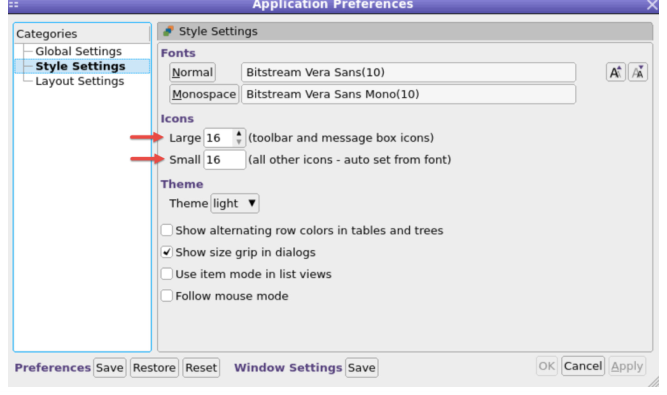
\includegraphics[width=0.92\textwidth]{gui-fig-001.png}
\caption{图标大小的应用程序首选项}
\label{fig:gui-1}
\end{figure}

\begin{figure}[htbp]
\centering
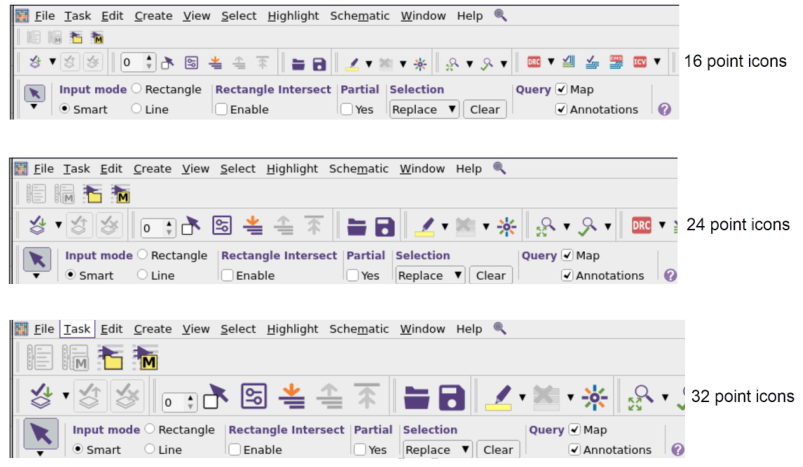
\includegraphics[width=0.92\textwidth]{gui-fig-002.png}
\caption{使用 16、24 与 32 点图标显示的工具栏}
\label{fig:gui-2}
\end{figure}

\subsection{选择浅色或深色显示主题}
\subsubsection*{Selecting a Light or Dark Display Theme}

要把背景从默认的浅灰主题改为深灰主题，选择 \textbf{View > Preferences > Style Settings}，并在 Theme 框中选择 dark。图~\ref{fig:gui-3} 同时给出浅色与深色主题。

\begin{figure}[htbp]
\centering
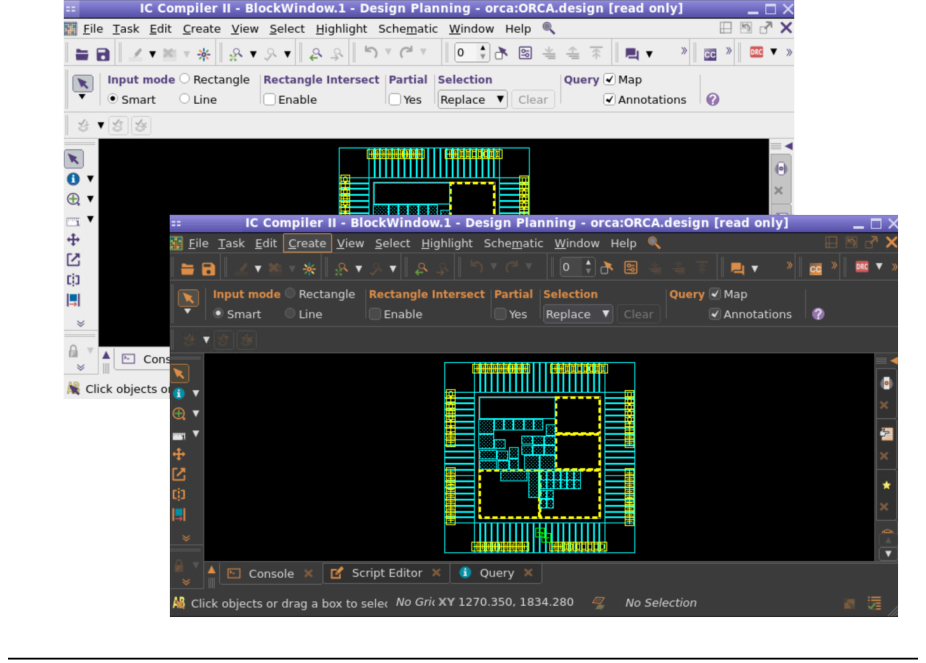
\includegraphics[width=0.92\textwidth]{gui-fig-003.png}
\caption{浅色与深色主题}
\label{fig:gui-3}
\end{figure}

% ============================================================
\section{使用命令搜索}
\subsection*{Using Command Search}

IC Compiler II GUI 提供命令搜索功能，用于快速定位菜单与任务操作、shell 命令以及应用选项。

要搜索命令：
\begin{enumerate}
  \item 单击菜单栏上的放大镜图标。
  \item 在表单顶部的 Search for: 部分单击一个或多个选项。
  \item 单击搜索框，键入命令名或主题的若干字母，或键入以空格分隔的多个词，以返回匹配结果列表。
\end{enumerate}

键入时，工具根据第 2 步所选选项，返回与搜索词相关的菜单与任务操作、shell 命令以及应用选项列表。对于 shell 命令，工具搜索命令名与命令选项列表，并按匹配质量对搜索结果排序。命令名匹配在搜索结果中的位置高于命令选项匹配。将指针移到搜索结果中的项目上，可查看包含该结果信息的信息提示（infotip），如图~\ref{fig:gui-4} 所示。

\begin{figure}[htbp]
\centering
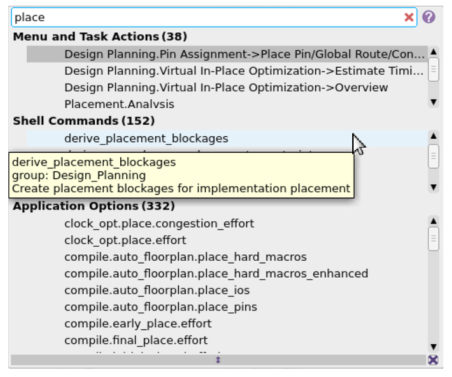
\includegraphics[width=0.92\textwidth]{gui-fig-004.png}
\caption{命令搜索结果}
\label{fig:gui-4}
\end{figure}

命令搜索支持对搜索框中一个或多个搜索词做完全匹配或部分匹配。例如，要搜索与块整形（block shaping）相关的结果，可以输入 “shape”、“block”、“sha bl”、“\cmd{shape\_blocks}” 等。若工具返回大量结果，右侧会显示滚动条以浏览列表。也可以编辑搜索词以缩小搜索结果。最后，单击列表中与搜索匹配的项目。

单击 Menu and Task Actions 列表中的项目即可运行该项。若该操作有对话框或面板，工具会打开它。若单击 Shell Commands 部分中的项目，工具会动态生成对话框。更多信息见本节「使用命令对话框（Using the Command Dialog）」。

若单击 Application Options 列表中的项目，工具打开 \textbf{Application Options} 对话框并显示所选应用选项。按需要设置该应用选项的值，单击 OK 保存更改，或单击 Cancel 保持该选项不变。也可以从菜单栏选择 \textbf{File > Application Options} 打开 \textbf{Application Options} 对话框。

使用命令搜索时，工具会记住当前工具会话中的搜索词以及你选择的操作。工具在 Recently found 部分显示以往选择的历史，在 Recently searched 部分显示本会话的搜索词。单击 Recently found 部分中的项目可再次执行该操作，或单击 Recently searched for 部分中的项目以重复该搜索。

命令搜索工具还支持下列附加功能：
\begin{itemize}
  \item 单击搜索框右侧的书本图标，用 Web 浏览器打开指向 SolvNetPlus 的链接，以搜索该搜索词。
  \item 单击搜索框右侧的 (X)，清除搜索框中的任何文本（仅当搜索框中含有文本时）。
  \item 按 Tab 键，在搜索栏与命令搜索工具的三个部分之间移动焦点。
  \item 将指针悬停在 Menu and Task Actions 部分与 Shell Commands 部分之间，或悬停在 Shell Commands 与 Application Options 部分之间，以显示分隔条；单击并拖动分隔条可调整该部分的大小。
  \item 单击并拖动命令搜索工具底部的条，以调整对话框大小。
  \item 单击命令搜索工具外部，或按 Esc 键，以关闭该工具。
\end{itemize}

\subsection{使用命令对话框}
\subsubsection*{Using the Command Dialog}

在 IC Compiler II 工具中，图形用户界面为工具中的 Tcl 命令即时生成对话框。在命令搜索的 Shell Commands 列表中单击某项时，工具为该命令生成对话框，如图~\ref{fig:gui-5} 所示。

\begin{figure}[htbp]
\centering
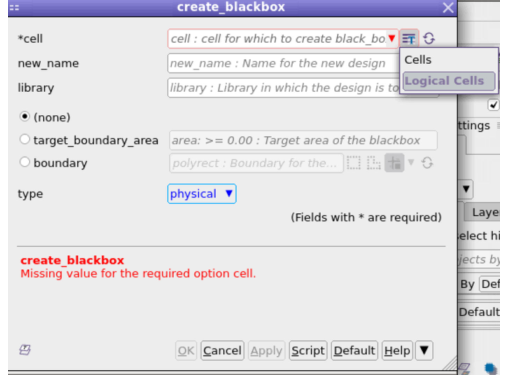
\includegraphics[width=0.92\textwidth]{gui-fig-005.png}
\caption{命令对话框}
\label{fig:gui-5}
\end{figure}

对话框在顶部列出选项与数据输入字段，在底部显示状态信息与命令预览。底行包含与此对话框相关的任务按钮。

在顶部，对话框中的必填字段以星号（*）标记。在文本框中键入时，工具校验输入。若输入中未检测到错误，工具以蓝色显示文本并更新命令预览。若输入包含错误，工具以红色显示文本，并在命令预览区域显示错误消息。单击 Default 按钮可恢复对话框中的默认值。要了解某个文本框的用途，将指针悬停在该框上以查看信息提示。

也可以在命令对话框中输入 Tcl 表达式与变量。例如，可以在图~\ref{fig:gui-5} 的 cell 文本框中输入下列内容：
\begin{itemize}
  \item 实际的单元名，例如 \cmd{u0\_0}
  \item \cmd{\$cell} 变量，用于指定你已定义的、包含单元名的变量
  \item Tcl 表达式，例如 \cmd{[get\_cells u0\_0]}
\end{itemize}

在可能的情况下，对话框提供用于选择边界框、层以及枚举值的工具，以帮助指定命令。要指定边界，执行下列操作之一：
\begin{itemize}
  \item 要定义矩形边界，选择相应按钮，然后在 Coordinates 框中输入矩形左上角与右下角的 $x$ 与 $y$ 坐标，或在版图视图中拖动指针，在所需位置形成矩形。
  \item 要定义直角多边形边界，选择相应按钮，然后在 Coordinates 框中输入每个拐角或方向变化处的 $x$ 与 $y$ 坐标，或在版图视图中拖动指针，在所需位置形成多边形各边。
  \item 要手动输入坐标，单击相应按钮，并在 Coordinates 框中输入矩形左上角与右下角的 $x$ 与 $y$ 坐标。
  \item 要启用或禁用网格吸附，选中或取消相应按钮。
  \item 要从列表中选择选项，单击相应按钮，并在出现的菜单上选择一项。
\end{itemize}

若命令选项要求指定一个或多个层，单击相应按钮并选择各层。也可以单击另一按钮并键入层名称。

若命令选项支持多个枚举值，单击相应按钮，并在出现的菜单上选择一项。对于所有其他表单输入项，在文本框中键入值。

在底部，工具提供用于执行不同操作的按钮：
\begin{itemize}
  \item 单击 OK 运行命令并关闭对话框。若对话框中存在错误，必须先纠正错误再单击 OK。
  \item 单击 Cancel 停止该命令。
  \item 单击 Apply 运行命令并保持对话框打开。
  \item 单击 Script 把命令复制到 Script Editor 窗口，而不运行该命令。
  \item 单击 Default 恢复对话框中的默认值。
  \item 单击 Help 在 Man Page Viewer 中打开该命令的 man 页。
\end{itemize}

% ============================================================
\section{使用主题搜索}
\subsection*{Using Topic Search}

工具提供界面，用于搜索安装目录中的帮助主题与其他文档。可搜索的文档包括 man 页、每日提示（tip of the day），以及通过菜单或单击按钮访问的 GUI 功能帮助主题。若搜索词包含在命令名、应用选项名、文档标题或文档关键字列表中，匹配项会出现在搜索结果中。请注意，该搜索工具不考虑通过 SolvNet 提供的在线文档。

要打开搜索工具：
\begin{enumerate}
  \item 选择 \textbf{Help > Man Pages}，打开 man 页查看器。\\
        第一次打开搜索工具时，工具显示用于查看 shell 命令、应用选项、错误消息、GUI 帮助以及每日提示主题的链接，如下图所示。
\end{enumerate}

\begin{figure}[htbp]
\centering
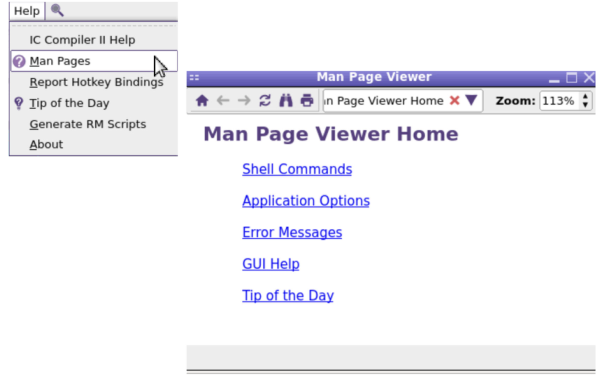
\includegraphics[width=0.92\textwidth]{gui-fig-006.png}
\caption{Man 页查看器}
\label{fig:gui-6}
\end{figure}

\begin{enumerate}
  \setcounter{enumi}{1}
  \item （可选）单击某个链接，查看该类别的目录。
  \item 在标题栏中输入搜索词，以显示与该词匹配的命令、应用选项和帮助主题。
\end{enumerate}

\begin{figure}[htbp]
\centering
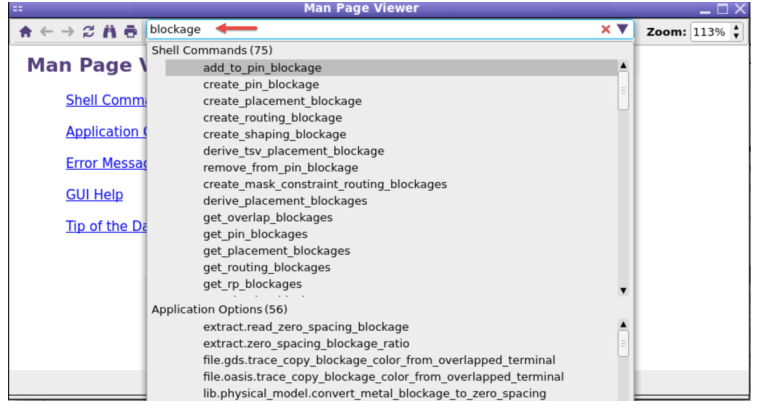
\includegraphics[width=0.92\textwidth]{gui-fig-007.png}
\caption{搜索词}
\label{fig:gui-7}
\end{figure}

\begin{enumerate}
  \setcounter{enumi}{3}
  \item 单击搜索框右侧的向下箭头，查看搜索历史。
\end{enumerate}

\begin{figure}[htbp]
\centering
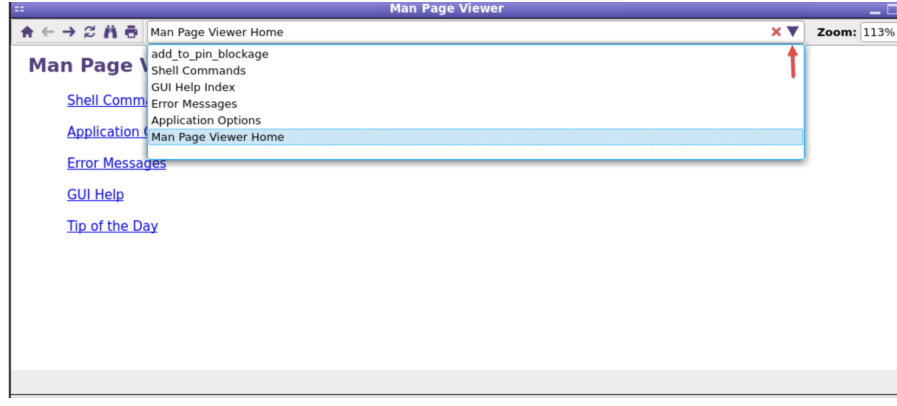
\includegraphics[width=0.92\textwidth]{gui-fig-008.png}
\caption{搜索历史}
\label{fig:gui-8}
\end{figure}

% ============================================================
\section{查看每日提示}
\subsection*{Viewing the Tip of the Day}

工具提供一组有用的提示，可用于改进工作流程。要查看每日提示，从菜单选择 \textbf{Help > Tip of the Day}。工具显示一条随机的每日提示。使用 Prev 与 Next 按钮查看更多提示。

% ============================================================
\section{创建参考方法学脚本}
\subsection*{Creating Reference Methodology Scripts}

面向 IC Compiler II 工具的 Synopsys 参考方法学（reference methodology）是一组脚本，其中收录了针对各厂商与工艺节点使用该工具的最新推荐方法。这些脚本是起点，可按你自己的设计需求加以改编和扩展。脚本中嵌有注释与备选设置，便于按需要定制流程。

要使用 GUI 为 IC Compiler II 工具生成 RM 脚本：
\begin{enumerate}
  \item 从菜单选择 \textbf{Help > Generate RM Scripts}。
  \item 为设计选择 Technology node。
  \item 为设计输入 Foundry 名称。
  \item 选择脚本的版本类型：Full RM 或 JumpStart。JumpStart 是新用户的起点，适用于已准备好执行 \cmd{place\_opt} 命令的块；这些脚本对扁平设计（flat design）运行推荐的默认布局布线（place-and-route）流程。
  \item 为脚本输入输出目录。默认情况下，压缩的 tar 文件写到当前目录。
  \item 单击 “I agree to the above Terms and Conditions.” 旁边的方框。
  \item 单击 OK。
\end{enumerate}

这些步骤把压缩的 tar 文件写到第 5 步指定的目录。写出文件后，使用 \cmd{tar xzf} \textit{filename} 命令解压文件。也可以用 \cmd{generate\_rm} 命令创建参考方法学脚本。

\begin{noteBox}
某些工艺节点需要晶圆厂提供的额外配置文件。请联系 Synopsys 代表，以获取这些文件方面的帮助。
\end{noteBox}

% ============================================================
\section{查看与编辑应用选项}
\subsection*{Viewing and Editing Application Options}

IC Compiler II 工具使用应用选项（application options）控制工具行为。为管理应用选项，IC Compiler II GUI 提供工具，用于显示当前应用选项设置、更改设置、把设置恢复为默认值，以及获取特定应用选项的帮助。

要打开应用选项工具，选择 \textbf{File > Application Options}，或在命令搜索结果中单击某个应用选项。

\begin{figure}[htbp]
\centering
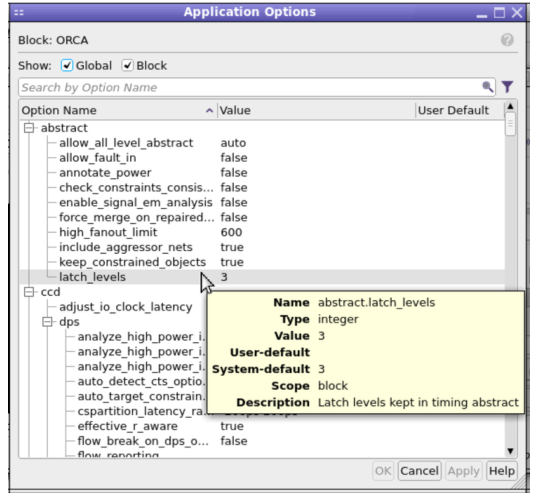
\includegraphics[width=0.92\textwidth]{gui-fig-009.png}
\caption{应用选项对话框}
\label{fig:gui-9}
\end{figure}

在 Tcl 命令中指定应用选项时，使用下列命名约定：
\begin{lstlisting}
category[.subcategory].option_name
\end{lstlisting}
其中 \cmd{category} 一般指受该应用选项影响的引擎。某些应用选项类别还有可选的子类别，用于进一步细化该应用选项所影响的范围。

应用选项具有全局作用域（global scope）或块作用域（block scope）。
\begin{itemize}
  \item 块作用域应用选项只应用于设置它们的那个块。它们保存在设计库中，并在多次工具会话之间保持。
  \item 全局作用域应用选项应用于所有块，但仅在当前会话内有效。它们不保存在设计库中；必须在每个 \cmd{icc2\_shell} 会话中指定。可以考虑把全局设置加入 \cmd{.synopsys\_icc2.setup} 文件。
\end{itemize}

\subsection{查看应用选项}
\subsubsection*{Viewing Application Options}

打开 \textbf{Application Options} 对话框后，工具显示当前的应用选项名称与设置。单击 Global 选项、Block 选项或两者，以选择要显示的应用选项作用域。要过滤应用选项列表，在搜索框中输入搜索词。键入时，工具过滤应用选项，只显示名称中包含该搜索词的选项。要按 Value 列过滤，输入 “Value:” 后接搜索词。例如，输入 “Value:true” 可只显示 Value 列中设置为 “true” 的应用选项。

要进一步限制列表中显示的应用选项，单击搜索框右侧的过滤按钮。取消 “Show if value is default”，以隐藏全部仍为默认值的应用选项设置。取消 “Show read-only”，以隐藏全部只读应用选项。

具有非默认设置的应用选项以粗体显示。将指针移到文本上可显示信息提示。信息提示给出选项名、选项类型、当前设置、用户默认设置、系统默认设置、作用域以及简短说明。

\begin{figure}[htbp]
\centering
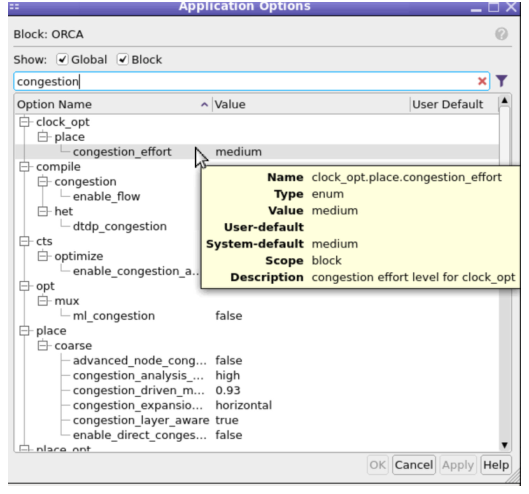
\includegraphics[width=0.92\textwidth]{gui-fig-010.png}
\caption{非默认选项}
\label{fig:gui-10}
\end{figure}

要显示某应用选项的 man 页，单击该选项以选中它，然后单击对话框右上角附近的按钮。工具打开所选应用选项的 man 页。

\subsection{编辑应用选项}
\subsubsection*{Editing Application Options}

要更改应用选项的值：
\begin{enumerate}
  \item 单击该选项值的文本。\\
        对于枚举类型与布尔类型选项，工具显示可能设置的列表。对于整数类型、浮点类型与文本选项，工具显示编辑框。
  \item 从列表中选择选项，或在文本框中输入新值。
  \item 单击 OK 保存设置并关闭对话框，或单击 Apply 保存设置。
\end{enumerate}

若应用了非默认设置，工具以粗体显示该应用选项及其设置。要把非默认设置恢复为其默认值：
\begin{enumerate}
  \item 单击选项值。
  \item 单击编辑框右侧的按钮，将该值设为其默认值。
  \item 单击 OK 或 Apply 以应用该设置。
\end{enumerate}

要把应用选项的值设为基于 Tcl 变量的值，按如下方式使用 \cmd{set\_app\_options} 与 \cmd{list} 命令：
\begin{lstlisting}
icc2_shell> set scriptdir "myscriptdir"
myscriptdir

icc2_shell> set_app_options \
   -list [list signoff.fix_drc.run_dir $scriptdir]
signoff.fix_drc.run_dir myscriptdir

icc2_shell> report_app_options signoff.fix_drc.run_dir
****************************************
Report : app_option
Design : ORCA
****************************************
Name                    Type   Value
----------------------- ------ -----------
signoff.fix_drc.run_dir string myscriptdir
----------------------- ------ -----------
1
\end{lstlisting}

% 第 1 章续：块窗口、视图与版图编辑
\section{在块窗口中工作}
\subsection*{Working in the Block Window}

启动 IC Compiler II 并打开 GUI 后，会出现块窗口（block window）。图~\ref{fig:gui-11} 标出块窗口的主要区域。

\begin{figure}[htbp]
\centering
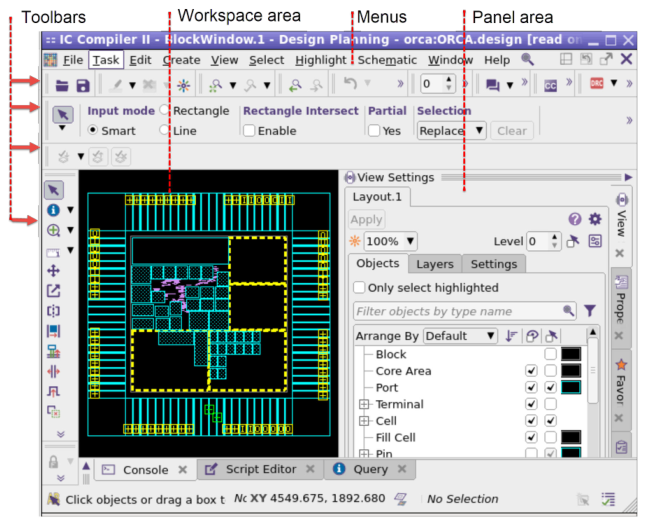
\includegraphics[width=0.92\textwidth]{gui-fig-011.png}
\caption{块窗口的主要功能区}
\label{fig:gui-11}
\end{figure}

打开一个块时，它显示在布局视图（layout view）中，这是该窗口的主块。再打开其他块时，每个块显示在各自的块窗口中。

块窗口是 GUI 的物理设计工作环境。布局视图是查看、分析与编辑块的中心。查看与编辑的细节见后文「更改物理设计的视图」与「编辑物理版图」。

\section{更改物理设计的视图}
\subsection*{Changing the View of the Physical Design}

布局数据往往很密，不同层上的对象互相重叠。可在 View Settings 面板上控制各类对象或各层的可见性（显示或隐藏）与可选性（允许或禁止选择）。也可定制对象或层的属性（颜色、填充图案等），并设置其他布局与对象显示选项。打开多个视图时，可为每个视图设置不同选项。

可用下列方式观察物理版图：
\begin{itemize}
  \item 设置并保存视图属性
  \item 在布局视图中显示网格线
  \item 绘制时序标尺
  \item 绘制物理标尺
  \item 绘制圆形标尺
  \item 用笔势（stroke）激活命令
\end{itemize}

\subsection{设置并保存视图属性}
\subsubsection*{Setting and Saving View Properties}

View Settings 面板用于设置当前活动视图的显示属性，也可把当前设置存入首选项文件，或从该文件加载设置。多个视图可各自使用不同选项。

显示 View Settings 面板：
\begin{itemize}
  \item 选择 \textbf{View > Toolbars > View Settings}；
  \item 或按 F8。
\end{itemize}

若面板被其他面板挡住，在面板区选择 View Settings 选项卡。

该面板可以：
\begin{itemize}
  \item 控制对象或层的可见性与可选性；
  \item 更改颜色、填充图案等样式；
  \item 设置视图或视图中对象的显示选项。
\end{itemize}

图~\ref{fig:gui-12} 是布局视图中对象页的 View Settings 面板。

\begin{figure}[htbp]
\centering
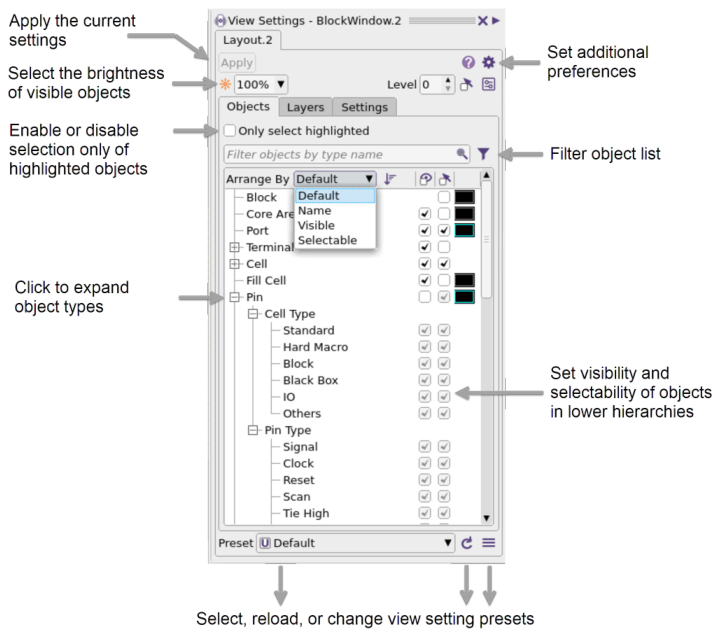
\includegraphics[width=0.85\textwidth]{gui-fig-012.png}
\caption{布局视图中对象的 View Settings 面板}
\label{fig:gui-12}
\end{figure}

设计对象的默认显示特性面向一般观察，对多数块已经合适。若要针对某个块或工作环境定制视图，可按对象类型单独修改。

显示或隐藏特定对象类型或层，可以只看关心的数据。启用或禁止某类对象或某层的选择，可以控制在视图中单击或拖拽时选中哪些对象。

改变样式属性可定制对象外观。可为单个对象类型或层设置颜色、填充图案、轮廓样式、轮廓宽度或夸张（exaggeration）值。

\begin{noteBox}
能改哪些属性，取决于该对象在视图中的图形表示。
\end{noteBox}

可以逐项设置，也可以套用一组预定义视图设置，称为 preset。既可使用工具提供的系统 preset，也可使用自己创建的自定义 preset。详见后文「应用预定义视图设置」。

更改活动布局视图的显示属性：
\begin{enumerate}
  \item 在 View Settings 面板上按需要设置选项。
  \item 单击 Apply。
\end{enumerate}

默认必须单击 Apply 才会生效。也可以让面板在修改后立即自动应用。单击 Options 按钮并选择 Auto apply，即可打开或关闭自动应用。要撤销尚未应用的修改，单击 Options 并选择 Cancel changes。

图~\ref{fig:gui-13} 是单击 Layers 选项卡后、用于设置层选项的面板。

\begin{figure}[htbp]
\centering
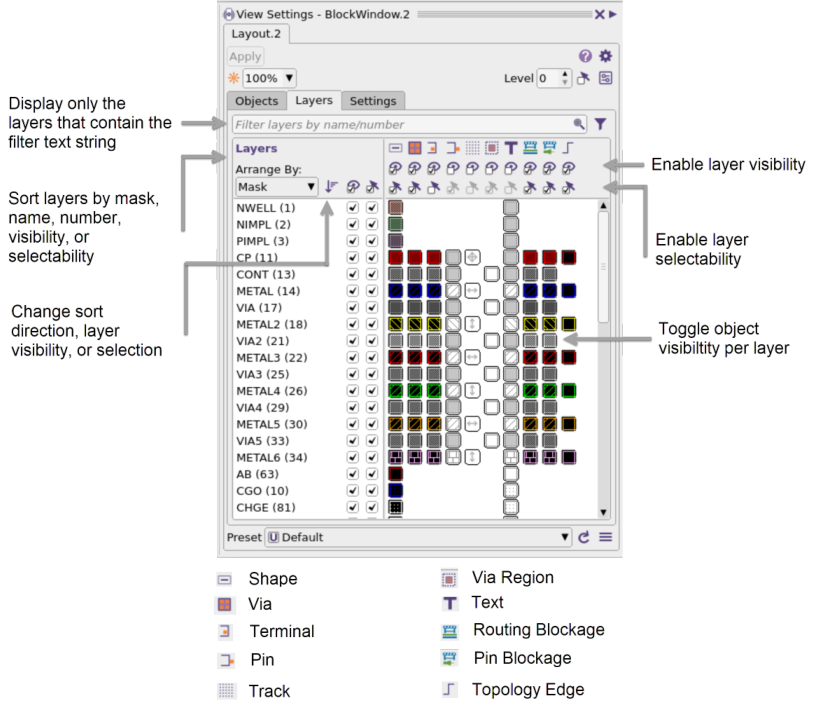
\includegraphics[width=0.85\textwidth]{gui-fig-013.png}
\caption{布局视图中层的 View Settings 面板}
\label{fig:gui-13}
\end{figure}

在层文本过滤框中输入字符串可过滤层列表。键入时，面板只显示名称中包含该文本的层；过滤只影响列表，不改变块窗口中的设计。单击文本框右侧的 (X) 可清除过滤。

单击 Arrange By 并选择排序方式，可按 mask、名称、层名、层号、可见性或可选性重排层列表。默认升序。单击 Arrange By 右侧的箭头可切换排序方向。

图~\ref{fig:gui-14} 是布局视图中 Settings 选项卡。该页有多个子页，用于设置视图、单元、线网、管脚、路径以及掩模颜色的显示选项。

\begin{figure}[htbp]
\centering
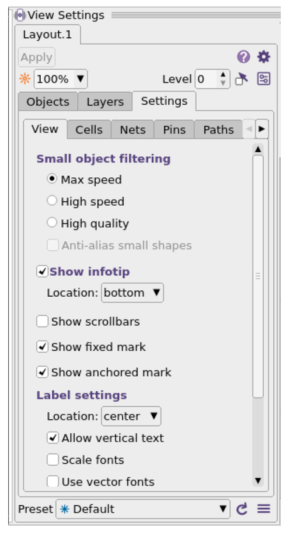
\includegraphics[width=0.55\textwidth]{gui-fig-014.png}
\caption{布局视图 Settings 页的 View Settings 面板}
\label{fig:gui-14}
\end{figure}

\subsubsection{保存与恢复视图设置}
\subsubsection*{Saving and Restoring View Settings}

退出会话时，工具不自动保存视图设置。若希望以后的会话沿用本次修改，可把它们写入首选项文件，之后再从该文件恢复。

保存活动视图的当前设置：在 View Settings 面板单击 Options，选择 \textbf{Preferences > Save To Preferences}。恢复最近一次保存的设置：单击 Options，选择 \textbf{Preferences > Set From Preferences}。

\subsubsection{应用预定义视图设置}
\subsubsection*{Applying Predefined View Settings}

preset 是一组预定义的视图属性。可以使用工具自带的系统 preset，也可以创建并应用自定义 preset。

打开块窗口时，工具默认使用首选项文件中保存的视图设置。要从 preset 应用设置，在 View Settings 面板底部的 Preset 列表中选择该 preset。例如，要套用面向设计规划的系统 preset，选择 floorplan。

在面板上手动改过设置后，Preset 列表中的名称前会出现星号（*）。若要重新套用该 preset 的设置，单击重新加载按钮。要把视图恢复为默认设置，在 Preset 列表中选择 Default。

创建自定义 preset 时要指定名称以及要包含的视图设置。可以新建，也可以重定义已有的自定义 preset，但不能重定义系统 preset。

创建自定义 preset：
\begin{enumerate}
  \item 单击相应按钮并选择 Save preset。出现 Write Layout Setting Preset 对话框。
  \item 选择已有 preset，或在 “Select or type a preset name” 框中输入新名称。
  \item 选择要包含的设置。对布局视图，默认包含 Objects 页的对象类型过滤与对象显示属性、Layers 页的层类型过滤，以及 Settings 页的布局显示设置。还可以选择包含 Layers 页的层显示属性，或 Objects 与 Layers 页的对象样式属性。
  \item 单击 OK。
\end{enumerate}

工具保存该 preset，并把名称加入 View Settings 面板的 Preset 列表。可以把某个 preset 指定为打开新块窗口或新视图时的默认配置。可以删除自定义 preset，不能删除系统 preset。

\subsection{在布局视图中显示网格线}
\subsubsection*{Displaying Grid Lines in a Layout View}

默认不显示网格线。可以显示光刻网格（lithography grid）或用户网格（user grid），以及 FinFET 网格。网格显示后，还可以在默认间距与十倍默认间距之间切换。
\begin{itemize}
  \item 显示或隐藏光刻网格：\textbf{View > Grid > Show Litho Grid}
  \item 显示或隐藏用户网格：\textbf{View > Grid > Show User Grid}
  \item 显示或隐藏 FinFET 网格：\textbf{View > Grid > Show Finfet Grid}
  \item 在默认间距与十倍间距之间切换：\textbf{View > Grid > Cycle grid spacing}
\end{itemize}

\subsection{在布局视图中绘制时序标尺}
\subsubsection*{Drawing Timing Rulers in a Layout View}

时序标尺（timing ruler）用于测量版图中两点之间的时序延时。延时来自 \cmd{read\_parasitic\_tech} 与 \cmd{set\_parasitic\_parameters} 设置的寄生参数，或来自 \cmd{set\_net\_estimation\_rule} 设置的线网估算规则。一条时序标尺可由一段或多段水平或垂直线段组成。默认在每段端点以及段内每第十个刻度处标注从标尺起点起算的延时。

\begin{noteBox}
绘制时序标尺的操作不能用 \textbf{Edit > Undo} 撤销。
\end{noteBox}

绘制步骤：
\begin{enumerate}
  \item 在 Mouse Tools 工具栏单击 Timing Ruler，或选择 \textbf{View > Mouse Tool > Timing Ruler}。启用后，Mouse Tool Options 工具栏出现相应选项，指针形状改变。默认会有十字标尺附着在指针上。
  \item （可选）在 Mouse Tool Options 工具栏设置选项：
  \begin{itemize}
    \item 选择 Attach，把标尺上的点吸附到对象；
    \item 在 Net Estimation Rule 中单击 Use 并选择规则名以计算时序；若不选，则按金属层与缓冲器尺寸计算；
    \item 选择水平层与垂直层；
    \item 更改利用率（utilization）；
    \item 更改缓冲器类型与间距；
    \item 指定非默认布线规则（NDR）；
    \item 更改标尺线段的网格吸附选项。
  \end{itemize}
  \item 在布局视图中单击标尺起点。若已选 Attach，指针经过对象时对象会高亮，标尺吸附到高亮对象。
  \item 单击该段终点。
  \item （可选）重复上述步骤再画一段。
  \item 按 Enter 结束这条标尺。
  \item （可选）重复上述步骤再画另一条标尺。
\end{enumerate}

单击定义标尺之前，可以打开或关闭 Attach，以限制能吸附的对象。可以删除单条标尺或视图中的全部标尺，但不能删除或修改单段线段。删除方法见下一节。

\subsection{在布局视图中绘制物理标尺}
\subsubsection*{Drawing Physical Rulers in a Layout View}

物理标尺用于测量距离，可由一段或多段水平、垂直或对角线段组成。默认在每段端点以及段内每第十个刻度处标注从标尺起点起算的距离。

绘制步骤：
\begin{enumerate}
  \item 在 Mouse Tools 工具栏单击标尺按钮，或选择 \textbf{View > Mouse Tool > Ruler}。启用后出现 Ruler Tool 选项，指针形状改变，默认有十字标尺附着在指针上。
  \item （可选）在 Mouse Tool Options 工具栏设置：
  \begin{itemize}
    \item 标尺模式。默认是两点模式（Two point mode），只画单段；要画多段，选择 Multi point mode；
    \item 方向选项；
    \item 是否显示附着在指针上的十字标尺、从标尺原点到各段端点的距离标签，以及各段中点处的段长标签；
    \item 标签距离的含义：相对设计原点的绝对坐标（Coordinate）、相对标尺原点的距离（Ruler Distance），或相对各段起点的距离（Segment Distance）；
    \item 线段的网格吸附；
    \item 是否把段长或距离记入会话记录（控制台日志）。
  \end{itemize}
  \item （可选）选择 Attach，把起点吸附到对象。
  \item 单击标尺起点。若已选 Attach，指针经过时对象高亮，标尺吸附到高亮对象。
  \item 单击该段终点。
  \item （可选）再画一段。
  \item 按 Enter 结束。
  \item （可选）再画另一条标尺。
\end{enumerate}

这样创建的标尺是持久的：保存设计并重新打开后，自动写入数据库的标尺仍然可用。对持久标尺可以移动、旋转、复制或拉伸。

与 GUI 操作对应的命令如下。

\begin{table}[htbp]
\centering
\caption{标尺相关命令}
\begin{tabularx}{\textwidth}{@{}l l X@{}}
\toprule
操作 & 命令 & 示例 \\
\midrule
新建标尺 & \cmd{create\_ruler} &
\cmd{create\_ruler -name example\_ruler -type ruler -color red -points \{\{123 456\} \{200 200\}\}} \\
查看设计中的标尺 & \cmd{get\_rulers} & \cmd{get\_rulers} \\
删除标尺 & \cmd{remove\_rulers} & \cmd{remove\_rulers} \\
把标注（含标尺）写成 Tcl & \cmd{write\_annotation\_shapes} &
\cmd{write\_annotation\_shapes -file recreate.tcl} \\
\bottomrule
\end{tabularx}
\end{table}

单击定义标尺之前，可以打开或关闭 Attach。可以删除单条或全部标尺，但不能删除或修改单段线段。

删除一条标尺：
\begin{enumerate}
  \item 单击标尺工具，或选择 \textbf{View > Mouse Tool > Ruler}。
  \item 把指针移到要删除的标尺上。
  \item 右键并选择 Remove Nearest Ruler。
\end{enumerate}

删除全部标尺：在 Mouse Tools 工具栏单击相应按钮，或选择 \textbf{View > Mouse Tool > Remove All Rulers}。

\subsection{绘制圆形标尺}
\subsubsection*{Drawing Circular Rulers}

可用 \cmd{gui\_add\_annotation} 创建圆形标尺。详见第~\ref{chap:gui-anno}~章「创建持久标注」。

\subsection{用笔势激活命令}
\subsubsection*{Using Strokes to Activate Commands}

在活动视图中拖动指针画笔势，可以激活预设命令。默认笔势用于：
\begin{itemize}
  \item 放大或缩小块；
  \item 平移块；
  \item 显示整个块。
\end{itemize}

也可以自定义笔势。基本笔势最多 72 种，多段笔势可以更多。

基本笔势是在布局视图中单击中键，或按住中键沿某一方向从一点拖到另一点。配合 Shift、Ctrl 或 Alt（或其组合）时，同一笔势可以激活其他命令。不按修饰键时，典型动作为：单击平移到中心、缩放到全图、矩形放大、矩形缩小等。按住 Ctrl 时，对应动作改为另一组缩放与平移，其中包括缩放到当前选择。

除基本笔势和带修饰键的笔势外，还可以做多段笔势。每一段可以是基本笔势所用的八个方向之一。

把命令绑定到基本或多段笔势，使用 \cmd{set\_gui\_stroke\_binding}。默认 GUI 使用基本笔势而不是多段笔势。用 \cmd{set\_gui\_stroke\_preferences} 可更改该首选项。具体用法见这两个命令的 man 页。

\section{编辑物理版图}
\subsection*{Editing the Physical Layout}

块窗口提供交互工具与命令，用于在库工作区中编辑块的版图。可以：
\begin{itemize}
  \item 移动、改变尺寸、复制和删除对象；
  \item 旋转、翻转对象，并改变单元方向；
  \item 改变对象形状；
  \item 对齐、分布和拉开对象；
  \item 扩展对象；
  \item 创建布线阻挡、线网形状、端口端子、文本对象和通孔。
\end{itemize}

通常先选中要编辑的对象。可以用选择工具交互选择，也可以在 Select By Name 工具栏输入名称。交互编辑工具处于活动状态时也可以选择对象。

选择工具有三种模式：Add、Replace 和 Remove。Add 与 Replace 是默认模式，Remove 是临时模式。按任意加速键可激活某个默认模式。用组合框在 Add 与 Replace 之间切换时，当前模式和默认模式一起改变。用组合框切到 Remove 时，只改变当前模式，默认模式不变，因此随后按键或松开按键会把当前模式恢复为 Add 或 Replace。

编辑工具可通过 Edit 或 Mouse Tools 工具栏上的按钮，或 Edit、Create 菜单打开。图~\ref{fig:gui-15} 给出这些工具栏和 Edit 菜单。相关编辑功能分组放在单击下拉箭头后展开的列表中。

\begin{figure}[htbp]
\centering
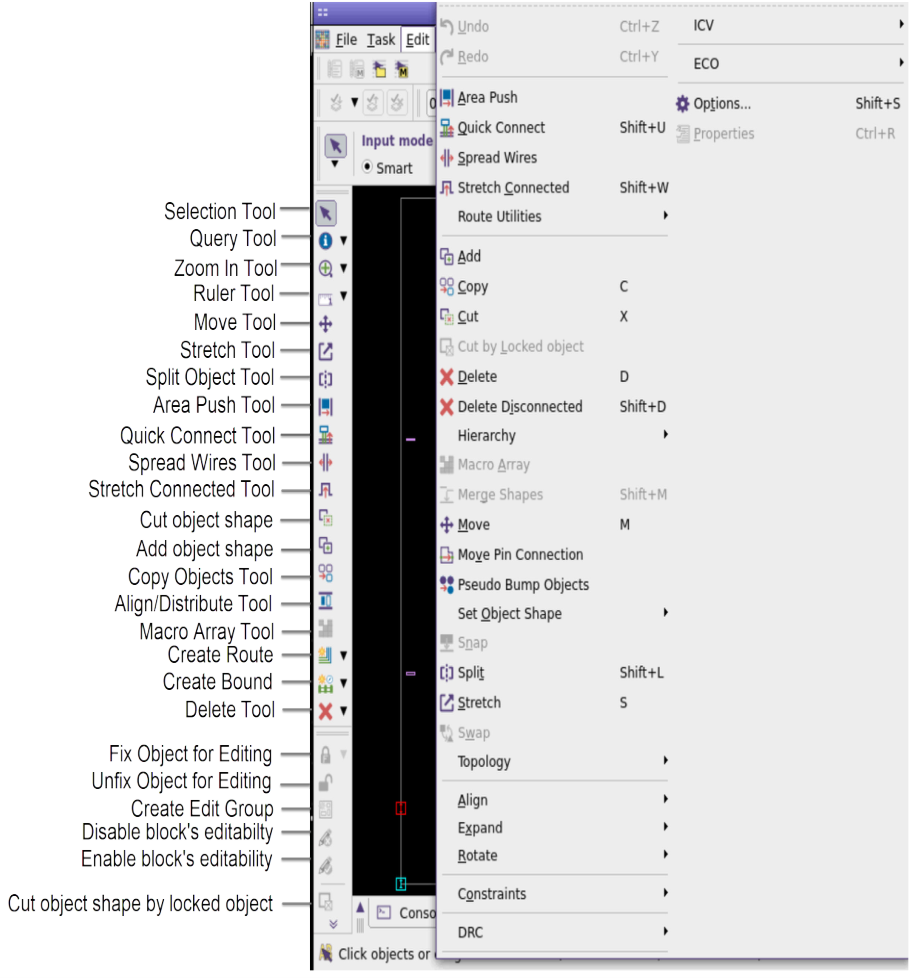
\includegraphics[width=0.92\textwidth]{gui-fig-015.png}
\caption{GUI 编辑命令}
\label{fig:gui-15}
\end{figure}

编辑物理对象与约束的进一步内容：
\begin{itemize}
  \item 交互编辑对象
  \item 在编辑环境中工作
  \item 使用 Editor Toolbox
  \item 使用就地编辑（edit in place）
\end{itemize}

\subsection{交互编辑对象}
\subsubsection*{Editing Objects Interactively}

版图编辑鼠标工具用于在布局视图中交互创建、编辑或删除物理对象。块窗口为所有工具提供一致的编辑环境。可以：
\begin{itemize}
  \item 在 Mouse Tool Options 工具栏设置工具选项；
  \item 用键盘快捷键做频繁或重复的操作；
  \item 预览待选对象，并在重叠对象之间循环。
\end{itemize}

编辑工具处于活动状态时，若要放大、浏览设计或测量距离，可以临时启用 Zoom In、Zoom Out、Pan 或 Ruler，而不必退出编辑工具。

在布局视图中激活某个鼠标工具后，其选项出现在 Mouse Tool Options 工具栏上。

表~\ref{tab:gui-edit-keys} 是交互编辑工具的标准按键。

\begin{table}[htbp]
\centering
\caption{交互编辑工具的按键约定}
\label{tab:gui-edit-keys}
\begin{tabularx}{\textwidth}{@{}X l@{}}
\toprule
动作 & 快捷键 \\
\midrule
单击或拖拽以添加点并执行操作 & Click 或 Drag \\
添加点并应用更改 & Return \\
删除最后一个点 & Backspace \\
取消尚未完成的输入，或退出工具 & Escape \\
在重叠对象中向前循环 & F1 \\
在重叠对象中向后循环 & Shift+F1 \\
撤销最近一次操作 & Ctrl+X \\
重做最近一次已应用的操作 & Ctrl+Y \\
\bottomrule
\end{tabularx}
\end{table}

许多编辑工具作用于已选对象。可以在激活工具之前或之后选择。激活编辑工具时若已有选择，Ctrl+单击把对象加入当前选择，Shift+单击把对象从当前选择中去掉。选中对象以选择色显示，默认是白色。

\begin{noteBox}
若难以选中或预览很小的对象，先放大视图。大设计在低倍率下，有些对象或轮廓小到无法点中。
\end{noteBox}

交互编辑工具能做的操作都会记入日志，并可用 \cmd{gui\_mouse\_tool} 重放。在 Mouse Tool Options 工具栏上设置的选项也会记入日志，并可用 \cmd{gui\_set\_mouse\_tool\_option} 重放。要查看某工具的命令与选项，单击帮助按钮打开该工具的 Help 页。

\subsubsection{移动、修改、创建与删除对象}
\subsubsection*{Moving, Modifying, Creating, and Removing Objects}

可以移动、改变尺寸、复制、拆分、整形、创建和删除对象。表~\ref{tab:gui-edit-tools} 列出常用工具。

\begin{table}[htbp]
\centering
\caption{设计对象的编辑工具}
\label{tab:gui-edit-tools}
\begin{tabularx}{\textwidth}{@{}l X@{}}
\toprule
操作 & 用法 \\
\midrule
移动对象 & \textbf{Edit > Move}，选中对象后单击或拖到新位置 \\
吸附到网格 & \textbf{Edit > Snap} \\
相对锚点对象或位置的边或中心对齐 &
\textbf{Edit > Align > Align/Distribute Tool}，在 Align 页选择对象、指定锚点，再单击对应对齐按钮 \\
相对锚点对象或位置的某一侧分布 &
同一工具的 Distribute 页，指定锚点后单击对应分布按钮 \\
改变尺寸 & \textbf{Edit > Stretch}，拖拽边或角 \\
复制 & \textbf{Edit > Copy}，选中后拖拽 \\
拆分 & \textbf{Edit > Split}，沿拆分位置拖一条线或一个矩形 \\
挖去一块并可选间隙来整形 &
\textbf{Edit > Cut}，可选设置间隙，再在对象上拖出矩形 \\
加上一块并可选间隙来整形 &
\textbf{Edit > Add}，可选设置间隙，再拖出矩形 \\
创建 bound & \textbf{Create > Bound}，拖出矩形 \\
创建布线阻挡 & \textbf{Create > Routing Blockage}，拖出矩形 \\
创建线网形状 & \textbf{Create > Shape}，拖出矩形 \\
创建端子 & \textbf{Create > Terminal}，指定管脚或端口后拖出矩形 \\
创建文本 & \textbf{Create > Text}，指定文字后单击位置 \\
创建通孔或通孔阵列 & \textbf{Create > Via}，单击位置 \\
删除对象 & \textbf{Edit > Delete}，单击或拖出矩形 \\
\bottomrule
\end{tabularx}
\end{table}

上述工具都可在 Mouse Tool Options 工具栏上按需要设置选项。

\subsubsection{扩展与旋转对象}
\subsubsection*{Expanding and Rotating Objects}

\begin{table}[htbp]
\centering
\caption{扩展、旋转与翻转}
\label{tab:gui-edit-xform}
\begin{tabularx}{\textwidth}{@{}l X@{}}
\toprule
操作 & 做法 \\
\midrule
把所选对象向一侧或全部方向扩展 &
单击扩展工具，或选择 \textbf{Edit > Expand > }\textit{direction}；也可使用 \cmd{expand\_objects} \\
将所选对象旋转 90 度或 180 度 &
单击旋转工具，或选择 \textbf{Edit > Rotate}；也可使用 \cmd{rotate\_objects} \\
沿 x 轴或 y 轴翻转 &
单击翻转工具，或选择 \textbf{Edit > Rotate > }\textit{axis}；也可使用 \cmd{flip\_objects} \\
\bottomrule
\end{tabularx}
\end{table}

\subsection{在编辑环境中工作}
\subsubsection*{Working in the Editing Environment}

编辑环境提供增量撤销与重做，可以回退或重新应用最近一次或一系列编辑。编辑时还可以固定（fix）对象、控制网格吸附、设置编辑选项，以及查看和编辑对象属性。表~\ref{tab:gui-edit-global} 是对任何编辑工具都可用的全局操作。

\begin{table}[htbp]
\centering
\caption{全局编辑操作}
\label{tab:gui-edit-global}
\begin{tabularx}{\textwidth}{@{}l X@{}}
\toprule
操作 & 用法 \\
\midrule
撤销上一次编辑 & 单击撤销按钮，或 \textbf{Edit > Undo}，或 \cmd{undo} \\
重做随后的编辑 & 单击重做按钮，或 \textbf{Edit > Redo}，或 \cmd{redo} \\
固定所选对象，避免交互编辑改动它 & \textbf{Edit > Constraints > Fix} \\
取消固定，允许交互编辑改动它 & \textbf{Edit > Constraints > Unfix Edit} \\
启用或关闭网格吸附 &
\textbf{Edit > Options}，在 Snapping 页选中或取消 Snapping enabled \\
查看或编辑所选对象的属性 & \textbf{Edit > Properties} \\
\bottomrule
\end{tabularx}
\end{table}

\subsection{使用 Editor Toolbox}
\subsubsection*{Using the Editor Toolbox}

Editor Toolbox 把移动、旋转、对齐、分布、拉开等常用编辑集中在一处。选择 \textbf{View > Assistants > Editor Toolbox} 打开它，见图~\ref{fig:gui-16}。

\begin{figure}[htbp]
\centering
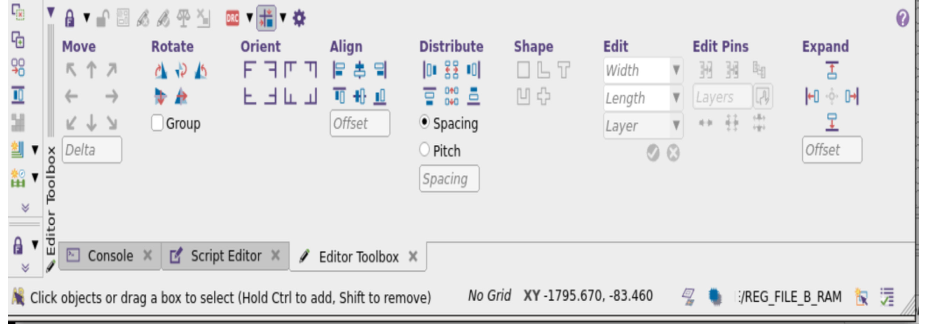
\includegraphics[width=0.92\textwidth]{gui-fig-016.png}
\caption{Editor Toolbox}
\label{fig:gui-16}
\end{figure}

\subsubsection{用 Editor Toolbox 编辑管脚}
\subsubsection*{Editing Pins With the Editor Toolbox}

可用 Editor Toolbox 对块管脚做移动、分布、对齐等操作。

\begin{table}[htbp]
\centering
\caption{管脚编辑操作}
\label{tab:gui-pin-edit}
\begin{tabularx}{\textwidth}{@{}l X@{}}
\toprule
操作 & 用法 \\
\midrule
允许编辑某块上的管脚 &
单击对应按钮，或 \cmd{set\_editability -blocks [get\_selection] -value true} \\
禁止编辑某块上的管脚 &
\cmd{set\_editability -blocks [get\_selection] -value false} \\
合法化所选块管脚，或与所选线网、单元相连的块管脚 &
\cmd{place\_pins -legalize} \\
从当前设计中删除所选端子 & \cmd{remove\_terminals} \\
对齐所选管脚 &
单击对齐按钮。后两个按钮还会分别按层属性改变层宽与层高。对应命令为 \cmd{align\_pins}、\cmd{align\_pins -change\_layer\_width}、\cmd{align\_pins -change\_layer\_height} \\
改变所选管脚宽度 & 在 Edit 区的 Width 框输入新值，单击对勾确认 \\
改变所选管脚长度 & 在 Length 框输入新值后确认 \\
改变所选管脚所在层 & 在 Layer 框选择新层后确认 \\
改变管脚排列 &
选中管脚后单击图标，设为 stacking、interleaving 或 reduce\_crossing。也可在 Design Assistant 的 Pins 页选择管脚，再选 \textbf{Edit > Pin Arrangement} \\
\bottomrule
\end{tabularx}
\end{table}

三种排列方式见图~\ref{fig:gui-17}。

\begin{figure}[htbp]
\centering

\includegraphics[width=0.28\textwidth]{gui-fig-017.png}\hfill

\includegraphics[width=0.28\textwidth]{gui-fig-018.png}\hfill

\includegraphics[width=0.28\textwidth]{gui-fig-019.png}
\caption{管脚排列：stacking（左）、interleaving（中）、reduce crossing（右）}
\label{fig:gui-17}
\end{figure}

\subsection{使用就地编辑}
\subsubsection*{Using the Edit in Place Functionality}

就地编辑（edit in place）让你在顶层上下文中编辑子块。它把当前块切换为所选块。可以下推（push）进入所选块，再上弹（pop）回来，也可以设置要查看的层次深度。工具栏见图~\ref{fig:gui-20}。

\begin{figure}[htbp]
\centering
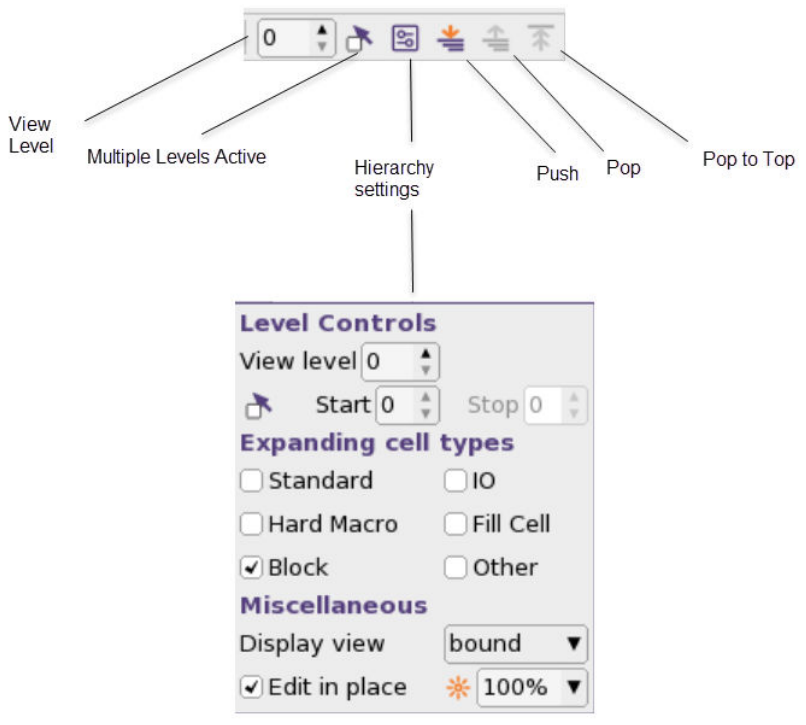
\includegraphics[width=0.92\textwidth]{gui-fig-020.png}
\caption{Edit in Place 工具栏}
\label{fig:gui-20}
\end{figure}

编辑子块：
\begin{enumerate}
  \item 选中要编辑的子块。
  \item 在 Edit in Place 工具栏单击 Push。\\
        下推时工具自动执行 \cmd{set\_working\_design -push}。例如：
\begin{lstlisting}
icc2_shell> set_working_design -push [get_cells \
   I_ORCA_TOP/I_BLENDER_1]
\end{lstlisting}
        可在控制台用 \cmd{current\_block} 核对当前块。
  \item 设计中的其他块会被变暗。用工具中的 dimness 图标调节变暗程度。设为 100\% 则周围块不变暗；设为 Off 则完全隐藏周围块。
  \item 按 F 键全屏缩放到新的当前块。
  \item 在子块上做编辑。
  \item （可选）若设计有多层，可再次 Push，进入更深层的特定对象。
  \item （可选）单击 Pop，向上返回一层。上弹时自动执行 \cmd{set\_working\_design -pop}。
  \item （可选）单击 Pop to Top，回到顶层（level 0）。此时自动执行：
\begin{lstlisting}
icc2_shell> set_working_design -pop -level 0
\end{lstlisting}
  \item （可选）按 Ctrl+F 查看完整设计。
  \item 用 Edit in Place 工具栏改变编辑层次、下推或上弹。
\end{enumerate}

\section{查看金属填充数据}
\subsection*{Viewing Metal Fill Data}

IC Compiler II 支持在同一上下文中编辑设计与金属填充（metal fill）数据。要启用金属填充编辑，打开 View Settings 面板并按图~\ref{fig:gui-21} 修改金属填充设置。金属填充在块内显示为一个或多个填充实例，数据与块一起保存在库中。要编辑这些数据，在 View Settings 面板中启用 All Levels Active。

\begin{figure}[htbp]
\centering
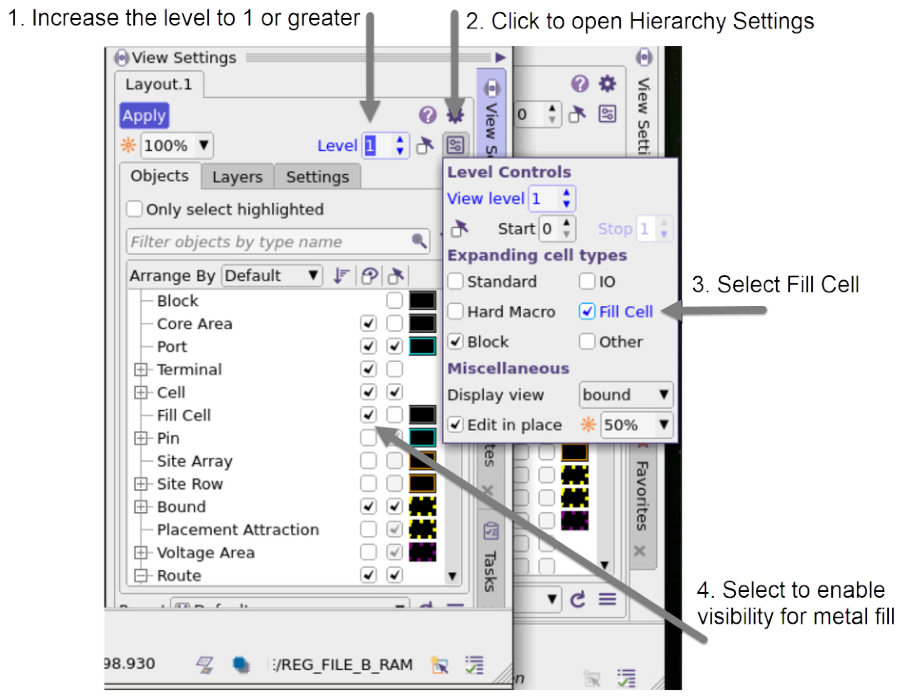
\includegraphics[width=0.85\textwidth]{gui-fig-021.png}
\caption{金属填充显示设置}
\label{fig:gui-21}
\end{figure}


% 第 2 章 Using Toolbars and the Selection List
\bichapter{使用工具栏与选择列表}{Using Toolbars and the Selection List}
\label{chap:gui-toolbar}

IC Compiler II GUI 提供用于查询信息、编辑并录制脚本以及完成其他任务的工具。

以下主题介绍 GUI 所支持的设计规划任务：
\begin{itemize}
  \item 使用查询工具
  \item 使用最近菜单按钮
  \item 使用脚本编辑器
  \item 使用按名称选择工具栏
  \item 使用总览工具栏
  \item 使用选择列表与工作列表
  \item 使用用户表
\end{itemize}

\section{使用查询工具}
\subsection*{Using the Query Tool}

Query 面板显示当前布局视图（layout view）或原理图视图（schematic view）中对象的信息。把查询工具（Query tool）设为当前鼠标工具（mouse tool）后，该面板会自动打开。单击某个对象时，Query 面板显示该对象的属性信息。

激活查询工具：选择 \textbf{View > Mouse Tool > Query tool}，或单击 Mouse Tools 工具栏上的 Query tool 按钮。指针变为 Query Tool 指针，工具在布局窗口右侧打开 Query 面板。

\begin{figure}[htbp]
\centering
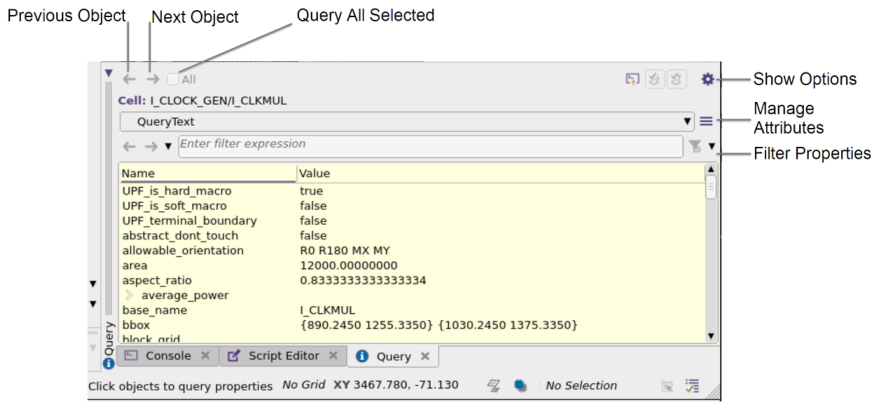
\includegraphics[width=0.92\textwidth]{gui-fig-022.png}
\caption{Query 面板}
\label{fig:gui-22}
\end{figure}

要显示某个对象的信息，单击该对象。工具会把该对象的信息填入 Query 面板。

要显示查询工具，并填入所选对象的信息，选择 \textbf{Select > Query Selection}。

要进一步控制 Query 面板中的信息显示，单击 Show Options 按钮并更改选项：
\begin{itemize}
  \item 选择 Auto Print Text to Log，则每次查询新对象时，把 Query 面板的内容写到控制台（console）。
  \item 选择 Auto Show when Query Tool is Chosen，则在 Query Tool 处于活动状态时，单击对象会自动打开 Query 面板。
  \item 单击 Customize Text，打开 Customize Query Toolbar 对话框。详见下文「使用定制查询工具栏」。
  \item 选择 Warn in selection exceeds size limit，并设置一个上限。选择规模超过该上限时，工具发出警告。
  \item 选择 Show attribute group，在 Query 面板中显示属性组（attribute group）选择框。
  \item 单击 Show attribute filter，在 Query 面板中显示文本过滤框。
\end{itemize}

在属性组框中选择一个属性组，则只显示属于该组的属性。要进一步了解某个组有哪些属性，单击属性组框右侧的 Activate Attribute Group Manager 按钮。属性组的说明见下文「使用属性组管理器」。

在过滤框中输入简单文本字符串，则只显示属性名中包含该文本的属性。要清除字符串，单击过滤文本框右侧的 (X)。单击过滤框右侧的 Filter properties 按钮，并选择 Show Read Only Properties，则只显示值为只读的属性。

单击 Name 或 Value 列标题，可更改该列的排序顺序。

\subsection{使用定制查询工具栏}
\subsubsection*{Using the Customize Query Toolbar}

要打开定制查询工具栏（Customize Query Toolbar），在 Query 面板的 Show Options 面板中单击 Customize Text。该工具栏见图~\ref{fig:gui-23}。

\begin{figure}[htbp]
\centering
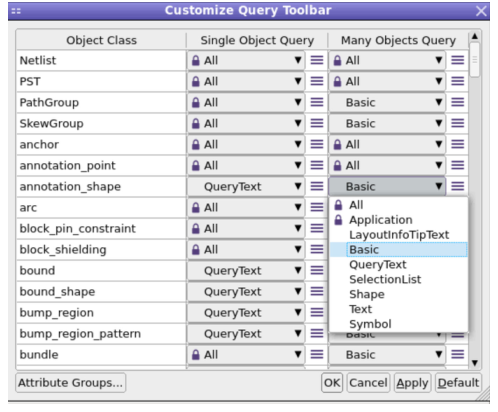
\includegraphics[width=0.55\textwidth]{gui-fig-023.png}
\caption{Customize Query Toolbar 对话框}
\label{fig:gui-23}
\end{figure}

Customize Query Toolbar 以表格显示对象类（Object Class）以及它们所属的属性组。要更改设置，单击 Single Object Query 或 Many Objects Query 列中的文本，并选择新值。选择 All，则该值会出现在所有组中。配置好列表后，单击 OK 或 Apply 使更改生效。

默认情况下，对象可以属于 Application、Basic、QueryText 等组。在 Query 面板中选中组名后，该对象类型的信息出现在 Query 面板的 Name 与 Value 列中。可以单击 Attribute Groups 按钮，用 Attribute Group Manager 对话框创建更多的组。详见下文「使用属性组管理器」。

\subsection{使用属性组管理器}
\subsubsection*{Using the Attribute Group Manager}

属性组管理器（Attribute Group Manager）用于定义新的属性组，以及向属性组添加对象或从中移除对象。

\begin{figure}[htbp]
\centering
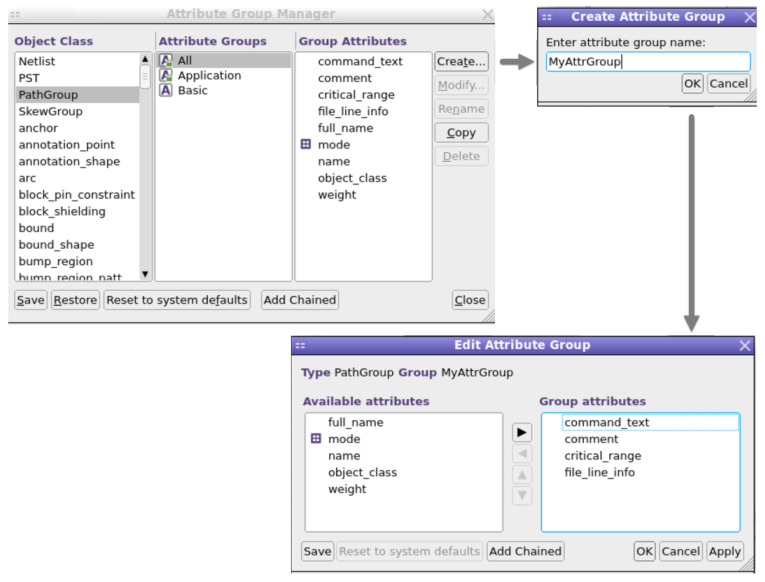
\includegraphics[width=0.85\textwidth]{gui-fig-024.png}
\caption{Attribute Group Manager 与 Attribute Group Editor}
\label{fig:gui-24}
\end{figure}

使用 Attribute Group Manager：
\begin{itemize}
  \item 单击 Create 创建新的属性组。在出现的对话框中输入属性组名称，单击 OK 保存。
  \item 单击某个 Object Class，再单击某个 Attribute Group 名称，然后单击 Modify，即可更改在 Query 面板中查询该对象时所显示的属性。详见下文「使用属性组编辑器」。
  \item 单击某个 Attribute Group 名称后再单击 Rename，或双击该 Attribute Group 名称，可重命名用户定义的属性组。系统定义的 Attribute Group 名称不能修改。
  \item 单击某个 Attribute Group 名称后再单击 Copy，可创建新的属性组，并把该组的属性复制到新属性组。
  \item 单击 Delete，从系统中移除所选的用户定义属性组。
  \item 单击 Save，把当前属性组设置写入 GUI 用户首选项文件。
  \item 单击 Restore，从 GUI 用户首选项文件读入属性组设置。
  \item 单击 Reset to system defaults，把应用程序定义的组内容恢复为默认值。用户定义的组不受影响。
\end{itemize}

\subsection{使用属性组编辑器}
\subsubsection*{Using the Attribute Group Editor}

属性组编辑器（Attribute Group Editor）用于向用户定义属性组的属性列表添加属性，或从中移除属性。在 Attribute Group Manager 中单击 Modify，即可打开 Attribute Group Editor。

按下列步骤修改所选属性组的属性列表：
\begin{itemize}
  \item 在左列选中一个属性，单击右箭头，把该条目移到右侧，使它可随此属性组一起显示。
  \item 在右列选中一个属性，单击左箭头，把该条目移到左侧，使它不在此属性组中使用。
  \item 在右列选中一个或多个条目，单击上箭头使条目在列表中上移；用下箭头使条目下移。
  \item 按 Control-A 选中该列中的全部条目。
  \item 单击 OK 保存结果，或单击 Cancel 退出对话框并且不保存。
\end{itemize}

\section{使用最近菜单按钮}
\subsection*{Using the Recent Menu Button}

最近菜单按钮（recent menu button）以图标和文字显示你在 GUI 中最近执行的操作。单击布局窗口左上方、当前鼠标工具图标下方的下箭头，即可显示该按钮，见图~\ref{fig:gui-25}。

\begin{figure}[htbp]
\centering
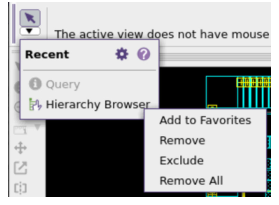
\includegraphics[width=0.4\textwidth]{gui-fig-025.png}
\caption{最近菜单按钮}
\label{fig:gui-25}
\end{figure}

在 GUI 中执行任务时，工具会在最近操作列表的顶部插入图标和文字。默认显示最近五条命令。单击 Show Options 按钮，为 Maximum Commands 选择新值，即可更改这个数目。

工具提供快捷键，用来调用最近使用的九条命令。按 Alt-1 调出最近一条命令，按 Alt-2 调出倒数第二条，其余依此类推。

可以右键单击，并从上下文菜单中选择下列选项，以修改最近使用命令的列表：
\begin{itemize}
  \item 选择 Add to Favorites，把该命令加入 Favorites 工具栏的命令列表。
  \item 单击 Remove，从最近使用命令列表中删除该命令。
  \item 单击 Exclude，删除该命令，并阻止它以后再进入此列表。要把命令从排除列表中移除，单击 Show Options 按钮，再单击 Reset Excluded。
  \item 单击 Remove All，从最近使用命令列表中移除全部命令。
\end{itemize}

单击 Show Options 按钮，可更改 Recent 工具栏的其他设置：
\begin{itemize}
  \item 用 Maximum Commands 为最近操作列表所保存的最大命令数选择新值。
  \item 单击 Reset Exclude，把全部命令从排除列表中移除。只有已经排除过一条或多条命令时，此按钮才可用。
\end{itemize}

\section{使用脚本编辑器}
\subsection*{Using the Script Editor}

脚本编辑器（Script Editor）用于在 IC Compiler II 中加载、编辑、运行和保存 Tcl 脚本。选择 \textbf{View > Toolbars > Script Editor} 即可激活。也可以把鼠标移到布局视图底部的状态栏，右键单击，从上下文菜单中选择 Script Editor。

\begin{figure}[htbp]
\centering
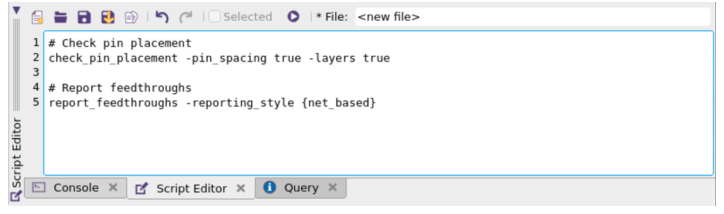
\includegraphics[width=0.85\textwidth]{gui-fig-026.png}
\caption{脚本编辑器}
\label{fig:gui-26}
\end{figure}

把指针移到图标上，信息提示（infotip）中会显示其功能。在 Script Editor 中可以做下列操作：
\begin{itemize}
  \item 单击 New，清除脚本窗口的内容。
  \item 单击 Open，在 Open 对话框中输入文件名，读入已有脚本。
  \item 单击 Save 保存脚本。
  \item 单击 Save As，用新文件名保存脚本。
  \item 单击 Undo，撤销对脚本的一处修改。
  \item 单击 Redo，反向最近一次撤销。
  \item 在搜索框中输入文本，单击 Find next 在文件中向前搜索；单击 Find previous 在脚本中向后搜索。
  \item 在搜索框中输入整数，单击 Go to line，把编辑器滚动到指定行号。
  \item 单击 Run Script，把脚本编辑器的内容保存到临时文件，并作为 Tcl 命令运行该文件。
  \item 用鼠标在脚本编辑器中选中单词或行，单击 Run Selection，把所选内容保存到文件并作为 Tcl 命令执行。
  \item 通过键入、剪切粘贴或删除文本，编辑脚本编辑器中的内容。
\end{itemize}

\section{使用按名称选择工具栏}
\subsection*{Using the Select By Name Toolbar}

按名称选择工具栏（Select By Name toolbar）按对象名称或搜索过滤表达式选择或高亮对象。选择 \textbf{Select > By Name Toolbar} 即可激活。也可以单击布局窗口左下角的 Select By Name 按钮。

\begin{figure}[htbp]
\centering
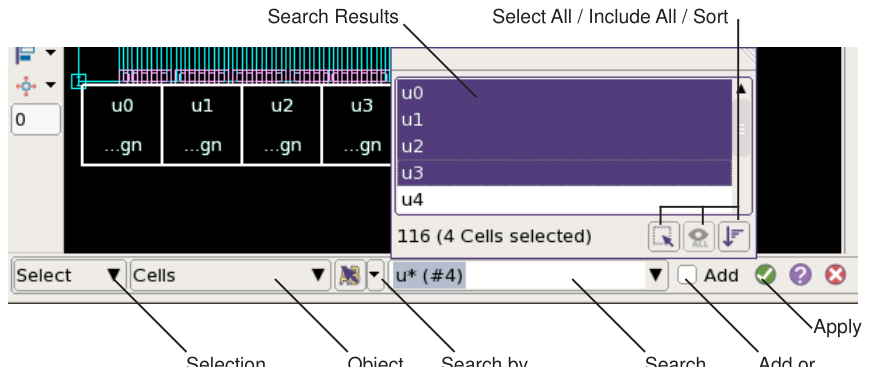
\includegraphics[width=0.92\textwidth]{gui-fig-027.png}
\caption{Select By Name 工具栏}
\label{fig:gui-27}
\end{figure}

该工具栏支持键盘快捷键，便于搜索并选择对象。使用 Select By Name 工具栏的典型流程如下：
\begin{enumerate}
  \item 按 Ctrl+/ 显示 Select By Name 工具栏。
  \item （可选）把选择模式改为 Highlight，以高亮（highlight）所选对象。
  \item （可选）从 Object Type 列表中选择对象类型。
  \item 按 F3 按名称搜索，或按 F4 按过滤器搜索。
  \item 输入与所找对象名称开头相匹配的部分搜索词。若没有匹配项，工具把输入框着成浅红色。
  \item 按 Tab，把搜索词扩展为匹配的对象名；若搜索词匹配多个对象，则显示全部匹配结果。
  \item 按 Insert，在 Add to Selection 与 Replace Selection 之间切换。
  \item 按 Enter 或单击 Apply，选中这些对象。
\end{enumerate}

\subsection{为多个对象输入搜索词}
\subsubsection*{Entering Search Terms for Multiple Objects}

搜索框提供灵活的界面，用来查找多个对象。要搜索多个对象名，用空格分隔搜索词。若对象名本身含有空格，用花括号 \cmd{\{\}} 分隔各项。按 Tab 键，搜索文本光标之前的那一项。要搜索另一项，移动光标后再按一次 Tab。单击搜索框右侧的 (X) 可清除搜索词。

若搜索词匹配多个对象，工具显示可滚动的搜索结果列表。继续键入，加长搜索词，以缩小结果范围。按上箭头键或下箭头键，在列表中向上或向下滚动。按 Enter 选中列表中的单个条目；按住 Control 键并单击其他结果，可把它们一并选中。单击 Select All 按钮，或按 Ctrl+A，选中列表中的全部结果。单击 Sort 按钮，反转列表的排序。按 Esc 退出列表。

在列表中选中多个对象后，搜索框显示缩写后的搜索词，例如 \cmd{(\#4)}，其中 4 是所选对象的个数。要在布局中选中这些对象，按 Enter。要把更多对象加入选择，单击 Add 选项或按 Insert，然后输入新的搜索词，并重复前面的步骤。

\subsection{按过滤器搜索}
\subsubsection*{Searching by Filter}

可以用 Select By Name 工具按过滤表达式搜索对象，见图~\ref{fig:gui-28}。

\begin{figure}[htbp]
\centering
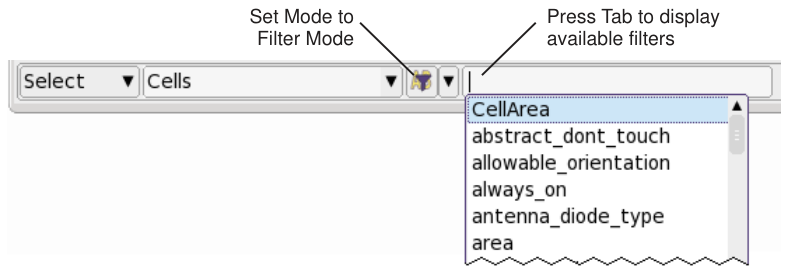
\includegraphics[width=0.85\textwidth]{gui-fig-028.png}
\caption{按过滤器选择}
\label{fig:gui-28}
\end{figure}

键入搜索表达式的前几个字母再按 Tab，即可快速构成过滤表达式。构成过滤搜索表达式的典型流程如下：
\begin{enumerate}
  \item 键入搜索表达式的前几个字母，例如 a。
  \item 按 Tab，显示与搜索表达式匹配的属性列表。
  \item 继续键入以缩小搜索范围，或单击列表中的属性。
  \item 再按 Tab，显示该属性的合法运算符。
  \item 继续键入以缩小搜索范围，或单击列表中的属性。
  \item 再按 Tab。若属性取枚举值（enumerated value），工具显示合法取值；否则在搜索框中插入一对空引号，或插入数值 0.0。
  \item 继续用 Tab 重复上述步骤，向表达式追加更多内容；或按 Enter 提交该表达式并执行搜索。
\end{enumerate}

\section{使用总览工具栏}
\subsection*{Using the Overview Toolbar}

总览工具栏（Overview toolbar）显示整个布局视图的轮廓，并用黄色高亮标出布局视图当前显示的区域。选择 \textbf{View > Toolbars > Overview}，即可激活总览工具栏并显示 Overview 面板。要在小弹出窗口中显示总览，单击布局窗口底部的 Overview 按钮。

\begin{figure}[htbp]
\centering
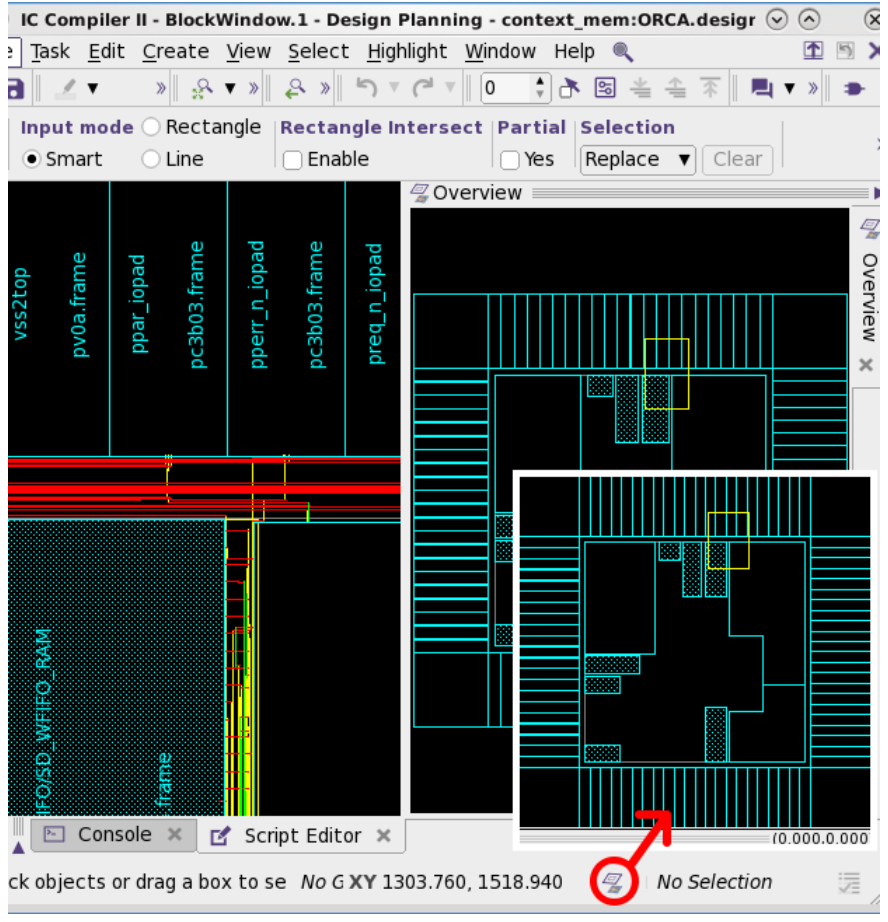
\includegraphics[width=0.92\textwidth]{gui-fig-029.png}
\caption{Overview 工具栏}
\label{fig:gui-29}
\end{figure}

要更改布局窗口中显示的设计区域，在总览面板或窗口中单击并拖拽黄色高亮区域。松开鼠标后，布局视图更新为高亮范围内的区域。

要更改布局视图的缩放倍数，把指针移到黄色高亮区域的边界。指针会变成可调整高亮大小的形状。单击并拖拽边缘，即可放大或缩小。

\section{使用选择列表与工作列表}
\subsection*{Using the Selection List and Work List}

选择列表（selection list）列出设计中当前选中的对象。若所选对象类型相同，选择列表显示这些对象的 Selection List 属性组。若对象类型不同，选择列表显示对象的 \cmd{name}、\cmd{object\_class} 与 \cmd{full\_name} 属性。

下图是选中了工作列表选项卡的 Selection List 对话框。

\begin{figure}[htbp]
\centering
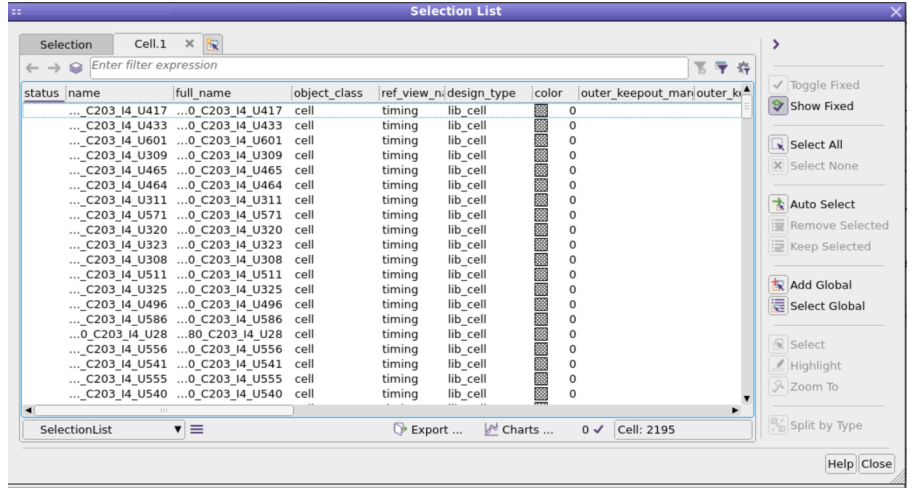
\includegraphics[width=0.92\textwidth]{gui-fig-030.png}
\caption{Selection List 对话框}
\label{fig:gui-30}
\end{figure}

选择列表中可以做下列操作：
\begin{itemize}
  \item 单击列标题，按该列对对象排序；再单击一次该标题，反转排序。
  \item 输入过滤表达式，减少列表中的条目。例如，下面的表达式只显示名称以 C 开头、朝向为 R270 的单元：
\end{itemize}

\begin{lstlisting}[language={}]
name=~C && orientation==R270
\end{lstlisting}

\begin{itemize}
  \item 单击过滤框旁的前后箭头，在以前用过的过滤表达式中向前或向后滚动。也可以单击过滤菜单按钮，查看全部过滤历史；单击列表中的一项，即用该表达式过滤列表。
  \item 单击 Toggle between filter expression 按钮，显示或隐藏各列自己的过滤器。
  \item 单击选项按钮，设置把过滤表达式解释为通配符表达式（wildcard expression）还是正则表达式（regular expression），以及多个表达式按 AND 组合还是按 OR 组合。
  \item 在属性组选择框中选择一项，为所选对象显示另一组列。默认显示 selection list 这一项。用 Attribute Group Manager 查看或修改某个属性组所显示的属性列表。
  \item 单击 Modify Attribute Group 按钮，以修改、管理或保存属性组。
  \item 单击 Charts 按钮，用图表分析设计数据。详见下文「图表」。
  \item 单击 Export 按钮，把列表或所选列表数据导出到 User Tables 导入表单，或导出为逗号分隔值（comma-separated values）文件。
\end{itemize}

\subsection{工作列表}
\subsubsection*{Work List}

工作列表（work list）是基于当前选择的持久对象列表。单击 Create Work List 选项卡按钮即可创建，此操作把当前选中的对象复制到工作列表。单击工作列表中的一项，会在当前布局、原理图或其他视图中自动选中该对象。工作列表的基本功能与选择列表相似，但在布局、原理图或其他视图中选择或取消选择对象时，工作列表保持不变。同一次工具会话中可以创建并管理多个工作列表，每个工作列表占用 Selection List 对话框中的一个选项卡。

工作列表选项卡中还可以做下列操作：
\begin{itemize}
  \item 选中一行或多行，单击 Toggle Selected Items Fixed 按钮，用勾号标记或取消标记这些项。
  \item 选中一行或多行，单击 Show/Hide Fixed Objects in List 按钮，显示或隐藏带勾号标注的行。
  \item 单击 Add Global Selection 按钮，把当前选中的项加入当前工作列表。
  \item 单击 Select Items to match Global Selection 按钮，在当前工作列表中选中那些同时在布局、原理图或其他视图中被选中的项。
\end{itemize}

\subsection{图表}
\subsubsection*{Charts}

要在图表中分析设计数据，单击 Selection List 对话框或工作列表选项卡中的 Charts 按钮，并从下列图表中选择：
\begin{itemize}
  \item Distribution plot：把一列的值划分到若干区间（bin）中，并显示每个区间内的值的个数。
  \item Box plot：按五数概括（five-number summary）显示一列或多列数值的分布。五数概括包括最小值（minimum）、第一四分位数（first quartile）、中位数（median）、第三四分位数（third quartile）与最大值（maximum）。位于 1.5 倍四分位范围（1.5 quartile range）之外的离群点（outlier）显示为单独的点。
  \item Scatter plot：在二维图中显示两列的值。
  \item Matrix plot：显示一组散点图。可以选择两列或多列，生成概括各列之间关系的图矩阵。
\end{itemize}

每个图表对话框都有上下文菜单，可对图执行常用操作。对话框中还包括：
\begin{itemize}
  \item 绘图区（plot area）
  \item 设置面板（settings panel）
  \item 数据表（data table，默认不显示）
  \item 状态栏（status bar）
\end{itemize}

可以指定图中使用的列、列分组（column group）、特定于该图的控件，以及选择行为的控件。

\section{使用用户表}
\subsection*{Using User Tables}

用户表（user table）用于导入、定义、交互操作并保存数据表。可以把用户表保存到设计数据库之外的文件中，并在以后的工具会话里重新加载。用户表可以由选择列表生成，也可以由逗号或制表符分隔的文件生成。

用户表支持许多常见的电子表格操作，例如编辑、排序、过滤、求和、查看列值分布等。此外，单击用户表中的行可以更改当前选择。

\subsection{创建用户表}
\subsubsection*{Creating a User Table}

从设计中已有的选择集创建用户表：
\begin{enumerate}
  \item 单击 Selection List 按钮，或选择 \textbf{Select > Selection List}，打开 Selection List 对话框。
  \item 单击 \textbf{Export > User Table}，按选择列表中的当前值创建用户表。\\
        工具把这些值复制到用户表导入表单。
  \item （可选）在 Table Name 框中更改表名。
  \item 单击 OK 导入数据并建立用户表。
\end{enumerate}

通过导入逗号或制表符分隔的文本文件创建用户表：
\begin{enumerate}
  \item 选择 \textbf{View > User Tables}。
  \item 单击用户表表单顶部附近的 Open 按钮。
  \item 在表单中选择分隔符（逗号或制表符）。需要时可以输入表名。
  \item 输入或选择文件名。
  \item 在 Configure Table Columns 表单中，按需要设置每一列的数据类型。
  \item 单击 OK 创建用户表。
\end{enumerate}

\subsection{保存与重新加载用户表}
\subsubsection*{Saving and Reloading a User Table}

保存用户表：
\begin{enumerate}
  \item 在表单顶部附近的 Action 框中选择 Save。
  \item 输入用于保存该数据库的文件名。用户表通常使用 \cmd{.utable} 扩展名。
  \item 单击 OK。
\end{enumerate}

工具把用户表数据写到指定文件。

加载已保存的用户表：
\begin{enumerate}
  \item 单击用户表表单顶部附近的 Open 按钮。
  \item 在 Select 下拉框中选择 Open UserTable file。
  \item 输入要加载的用户表文件名。
  \item 单击 OK。
\end{enumerate}

\subsection{分析用户表中的数据}
\subsubsection*{Analyzing Data in a User Table}

创建用户表之后，可以做下列操作：
\begin{itemize}
  \item 右键单击列标题，并选择上箭头或下箭头按钮，对该表排序或反向排序。
  \item 用下列方法之一过滤表：
  \begin{itemize}
    \item 单击过滤按钮；
    \item 在过滤栏中输入列迭代函数（iterator）与归约函数（reduction）。
  \end{itemize}
\end{itemize}

支持的函数包括：\cmd{approx()}、\cmd{abs()}、\cmd{round()}、\cmd{scale()}、\cmd{offset()}、\cmd{min()}、\cmd{max()}、\cmd{sum()}、\cmd{count()}、\cmd{avg()}、\cmd{mean()}、\cmd{median()}、\cmd{lower\_quartile()}、\cmd{uppper\_quartile()}、\cmd{stdev()}、\cmd{second\_stdev()} 与 \cmd{third\_stdev()}。

迭代函数的例子如下。它显示该表达式为真的所有行。用 \cmd{@column\_name} 语法引用列。

\begin{lstlisting}[language={}]
Tot Power > @Lkg Power
\end{lstlisting}

归约函数的例子如下。

\begin{lstlisting}[language={}]
Lkg\ Power > #mean(Tot\ Power)
\end{lstlisting}

下面的例子中，过滤查询显示某一行的 Tot Power 约等于同一行 Lkg Power 的 10\% 的所有行。

\begin{noteBox}
\cmd{approx()} 只能出现在表达式的右侧。
\end{noteBox}

还可以：
\begin{itemize}
  \item 单击并拖拽列标题，重排列的顺序。也可以右键单击列标题，选择 \textbf{More Column Options > Configure Columns}，打开 Configure Columns 对话框。
  \item 单击用户表表单顶部附近的 Tables 框并选择新的表名，以显示另一张用户表。
  \item 右键单击表中的单元格，选择 \textbf{Selection > Toggle Auto Select Mode}，再单击单元格，即可在布局或原理图视图中选择或取消选择当前对象。
\end{itemize}

\subsection{创建汇总报告}
\subsubsection*{Creating a Report Summary}

用户表中的汇总报告提供表列数据的基本统计。要为用户表生成汇总报告，在用户表表单顶部附近的 Action 框中选择 Report (summary)。工具显示表中数值列的统计量，包括最小值、最大值、平均值等。每一列的第一行给出该列数值与分类值的直方图（histogram）链接。

单击第一行中的任意链接，显示该列的分布报告。在分布报告中，单击列标题可按该列的值对表排序。在 Action 框中选择 Report (summary)，返回汇总报告。

\subsection{在用户表中自动选择对象}
\subsubsection*{Automatically Selecting Objects in a User Table}

可以用 Auto Select Object 下拉选项，让工具在用户表中自动选择对象。

默认选中 Objects defined by Column 与 None。其含义是：对于列中的某个值，工具按该列所定义的对象类型尝试选择对象。

若选择 Objects defined by object\_class，工具按对象类给出的对象类型，用 \cmd{full\_name} 列中的名称查找并选择对象。

\subsection{改进的总线压缩}
\subsubsection*{Improved Bus Compression}

可以压缩符合 \cmd{[*]} 总线记法、\cmd{[\#]}、\cmd{\_\#\_/} 或 \cmd{\_\#/} 的总线信号，其中 \# 为某个数字。

此选项可用于：
\begin{itemize}
  \item 任何含有线网、管脚、单元或时序点某种全名的列，作为列上下文菜单中的一项；
  \item hierarchy 视图与 Child List 视图。
\end{itemize}

该操作会创建一张用户表，把所有符合该总线记法的信号按总线合在一起。

单击 Show 列下方的某个链接，打开一张新的子表（child table），其中包含该总线上的各个信号。在这张子表中，若信号是时序路径的端点（endpoint），表中还可能有链接，用来查看时序路径点的子表。

用左上角的上下箭头，在下钻分析中生成的父表与子表之间来回切换。

\subsection{以图表或曲线查看数据}
\subsubsection*{Viewing the Data as a Chart or Plot}

要把用户表中的数据看成图表或曲线，使用列上下文菜单按钮 Select Plot。仅当所选列的数据包含数值时，该按钮才可用。

可以选中多列，再按用户表中这些列的数据创建图。

下图为生成的图。原稿未给出该图的 Figure 编号，图文件无法对应，故此处不插入图片。

要按列中的值过滤数据，把鼠标移到生成的图上并单击 Filter。可以用 Plot Control 定制并控制该图的各项选项。

要查看上次看过的图，单击 last viewed plot 工具按钮。只有此前查看过该表的图时，此按钮才可用。

% 第 3 章 Using GUI Assistant Tools
\bichapter{使用 GUI 助手工具}{Using GUI Assistant Tools}
\label{chap:gui-assist}

IC Compiler II GUI 提供多种助手，例如任务助手（Task Assistant）、线网助手（Net Assistant）、管脚助手（Pin Assistant）和设计助手（Design Assistant），用来管理设计中的不同对象。例如，任务助手把常用命令归集到不同流程中，以支持设计规划（design planning）、时序分析（timing analysis）、布局（placement）以及其他流程。GUI 助手工具可以简化设计过程。

本章说明如何使用这些 GUI 工具，包括以下主题：
\begin{itemize}
  \item 使用任务助手
  \item 使用设计助手
  \item 用相对位置约束工具设置约束
  \item 使用网表追踪器
  \item 使用布线轨道助手
\end{itemize}

\section{使用任务助手}
\subsection*{Using the Task Assistant}

任务助手便于浏览设计规划及其他流程，并执行单项任务来完成设计。以下几节说明任务助手的主要功能。

\subsection{启动 Tasks 工具栏与任务助手}
\subsubsection*{Starting the Tasks Toolbar and Task Assistant}

要打开 Tasks 工具栏，从菜单选择 \textbf{View > Toolbars > Tasks}。工具在版图视图（layout view）右侧显示任务面板，见图~\ref{fig:gui-31}。

\begin{figure}[htbp]
\centering
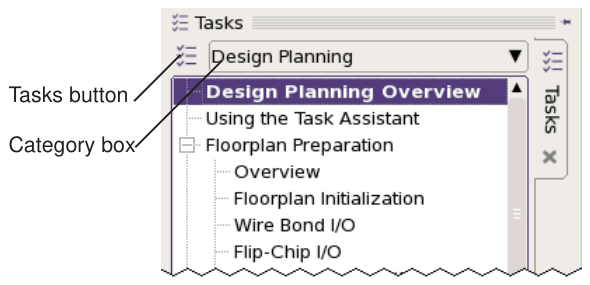
\includegraphics[width=0.92\textwidth]{gui-fig-031.png}
\caption{任务面板}
\label{fig:gui-31}
\end{figure}

要显示另一类别的任务列表，单击类别框（category box）右侧的向下箭头。要显示任务助手对话框，单击类别框左侧的 tasks 按钮。也可以从菜单选择 \textbf{Task > Task Assistant}。

\subsection{在任务助手对话框中浏览任务}
\subsubsection*{Navigating the Tasks in the Task Assistant Dialog Box}

任务助手对话框提供按钮，可转到任务列表中的下一项或上一项任务，也可在历史列表中后退或前进。任务助手窗口左侧是带目录（table of contents）的导航窗格（navigation pane）。在导航窗格中，选择左上角的类别，即可载入该类别的任务列表。单击导航窗格中的任一任务，即可把对应表单载入任务助手。单击导航窗格中的 [-] 图标可折叠任务子类，单击 [+] 图标可展开子类。图~\ref{fig:gui-32} 给出任务助手的部分导航功能。

\begin{figure}[htbp]
\centering
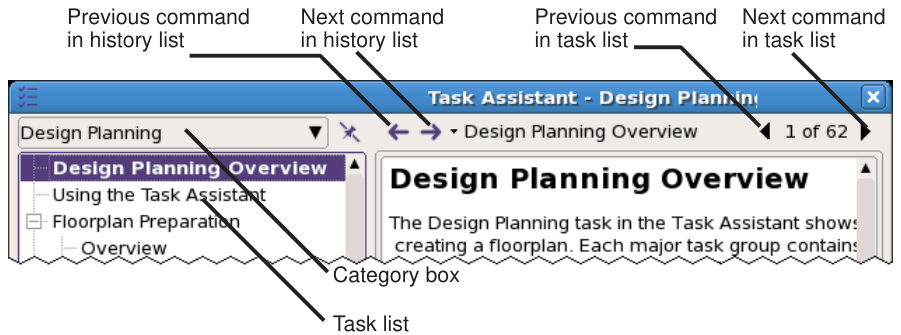
\includegraphics[width=0.92\textwidth]{gui-fig-032.png}
\caption{任务助手导航}
\label{fig:gui-32}
\end{figure}

若任务列表处于隐藏状态，如图~\ref{fig:gui-33} 所示，单击箭头将其打开，再单击图钉（pin）以显示任务列表。

\begin{figure}[htbp]
\centering
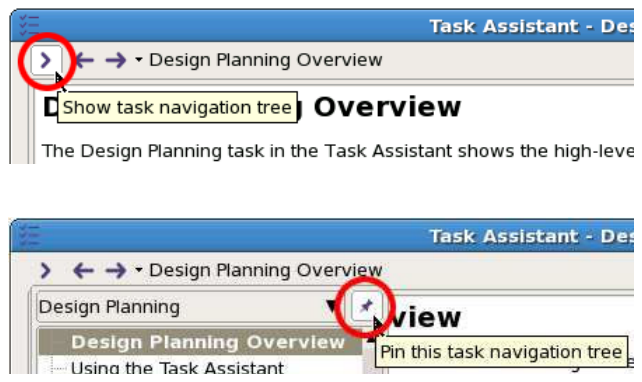
\includegraphics[width=0.92\textwidth]{gui-fig-033.png}
\caption{固定导航窗格}
\label{fig:gui-33}
\end{figure}

也可以把指针移到任务助手左侧，直到出现两条竖线。单击该竖线并向右拖动，即可显示导航栏，见图~\ref{fig:gui-34}。

\begin{figure}[htbp]
\centering
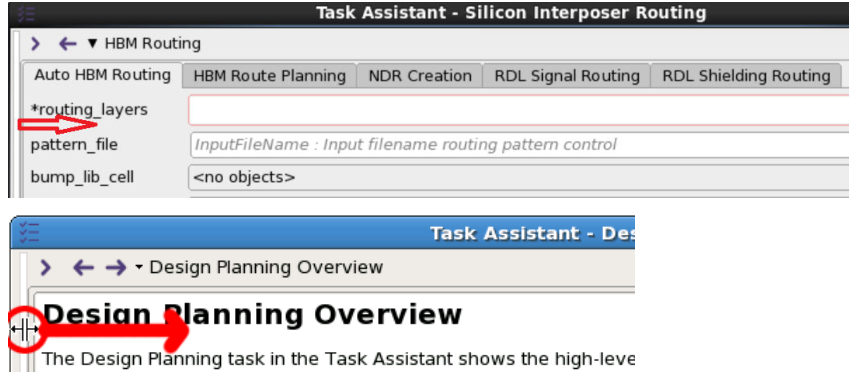
\includegraphics[width=0.92\textwidth]{gui-fig-034.png}
\caption{显示导航栏}
\label{fig:gui-34}
\end{figure}

\subsection{预览、捕获并执行命令}
\subsubsection*{Previewing, Capturing, and Issuing Commands}

填完表单数据后，查看表单底部附近的预览窗口，核对即将运行的命令，见图~\ref{fig:gui-35}。在表单中输入数据并选择选项时，该窗口会自动更新。根据某一项允许输入的数据类型，文本框可能会阻止输入不正确的信息。

\begin{figure}[htbp]
\centering
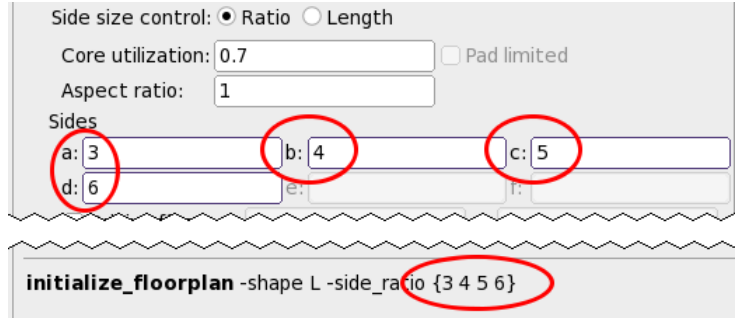
\includegraphics[width=0.92\textwidth]{gui-fig-035.png}
\caption{Tcl 命令预览窗口}
\label{fig:gui-35}
\end{figure}

改变选项或文本框中的内容，即可改变命令。单击 Script 按钮，把命令复制到 IC Compiler II GUI 版图窗口中的 Script Editor。可用 Script Editor 中的工具按需要编辑并保存该命令。

预览命令之后，单击 Apply 运行命令。若检测到命令语法有问题，工具会发出警告。若出现问题，改正表单后再试。

\subsection{使用概览页}
\subsubsection*{Using Overview Pages}

任务列表中的某些任务是在 GUI 面板中操作的。例如，Hierarchy Exploration 与 What-if Congestion Analysis 任务分别通过 GUI 中的 \textbf{View > Assistants > Hierarchy Exploration} 与 \textbf{View > Map > What-if Channel Congestion} 完成。对这些任务，任务助手提供概览页（overview page），帮助理解相应工具。图~\ref{fig:gui-36} 是 What-if Channel Congestion 的概览页。

\begin{figure}[htbp]
\centering
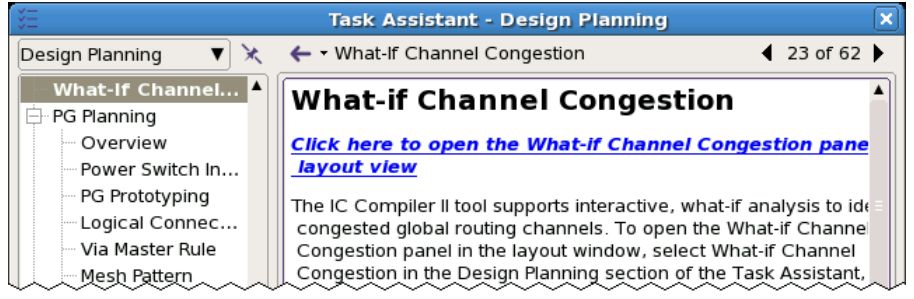
\includegraphics[width=0.92\textwidth]{gui-fig-036.png}
\caption{What-if Channel Congestion 概览页}
\label{fig:gui-36}
\end{figure}

单击页面顶部的链接，或按页面所述使用菜单命令，即可在 GUI 中打开该工具。按概览页中的说明完成该任务。

\begin{seeAlsoBox}
Hierarchy Exploration 与 What-if Channel Congestion 见第~\ref{chap:gui-dp}~章。
\end{seeAlsoBox}

\subsection{编辑表中的数据}
\subsubsection*{Editing Data in Tables}

对于设置或查看约束（constraint）信息的任务，任务助手提供可编辑的表，用于查看或修改约束数据。下列内容是 \textbf{Block Shaping > Shaping Constraints} 任务所显示的块列表，见图~\ref{fig:gui-37}。

\begin{figure}[htbp]
\centering
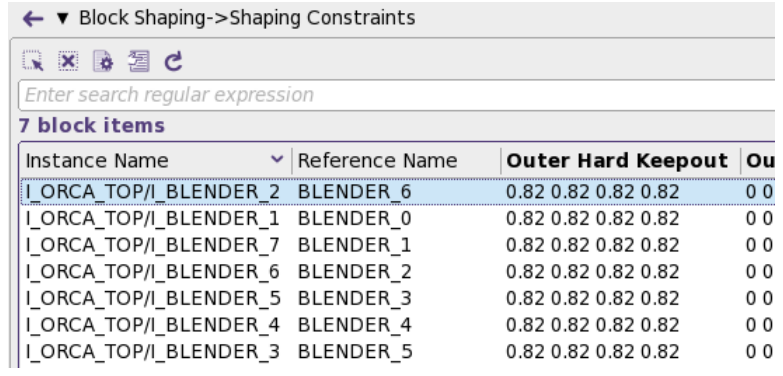
\includegraphics[width=0.92\textwidth]{gui-fig-037.png}
\caption{实例搜索}
\label{fig:gui-37}
\end{figure}

要编辑约束：
\begin{enumerate}
  \item 双击表中的一个单元格。
  \item 用 Backspace 键删除当前内容。
  \item 为该单元格输入新的约束。\\
        内容不完整或不正确时，工具以红色显示文本。有效值以黑色显示。
  \item 按 Return 键确认新值。
\end{enumerate}

编辑表单元格数据见图~\ref{fig:gui-38}。

\begin{figure}[htbp]
\centering
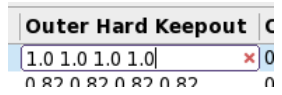
\includegraphics[width=0.92\textwidth]{gui-fig-038.png}
\caption{编辑表单元格数据}
\label{fig:gui-38}
\end{figure}

\section{使用设计助手}
\subsection*{Using the Design Assistant}

设计助手帮助在版图视图中定位并选择对象。要启动设计助手，从菜单选择 \textbf{View > Assistants > Design Assistant}，或单击 Design Assistant 按钮。界面见图~\ref{fig:gui-39}。

\begin{figure}[htbp]
\centering
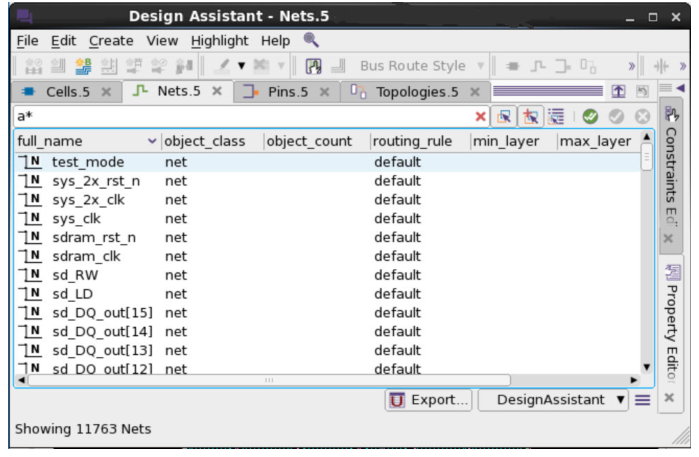
\includegraphics[width=0.92\textwidth]{gui-fig-039.png}
\caption{设计助手}
\label{fig:gui-39}
\end{figure}

以下几节说明如何使用设计助手。

\subsection{列出并选择对象}
\subsubsection*{Listing and Selecting Objects}

设计助手提供搜索框，用于列出单元、线网、管脚和拓扑（topology）对象。要填充对象列表：
\begin{enumerate}
  \item 单击 Cells、Nets、Pins 或 Topologies 选项卡。\\
        只有从上下文菜单（context menu）选择 Get Topology Plans，或使用菜单命令 \textbf{View > Topology Plans of selected} 或 \textbf{View > New Topologies} 时，Topologies 选项卡才可用。
  \item 在搜索框中输入搜索词。\\
        可以指定完整字符串、子串（substring）、通配符表达式（wildcard expression）、Tcl 命令或 Tcl 变量。例如，在搜索框中输入下列任一项，即可匹配单元 \cmd{u0\_0}、\cmd{u0\_1}、\cmd{u0\_2}、\cmd{u0\_3}（以及可能的其他单元）：
        \begin{itemize}
          \item 仅字符串：\cmd{'u'}、\cmd{'u0'} 或 \cmd{'u0\_'}
          \item 通配符：\cmd{'u0\_*'}、\cmd{'u0\_?'}
          \item Tcl 命令：
\begin{lstlisting}
get_cells "*" -filter name=~"u0*"
\end{lstlisting}
          \item Tcl 变量：\cmd{\$my\_cells}（先在工具中执行）
\begin{lstlisting}
set my_cells [get_cells "*" -filter name=~"u0*"]
\end{lstlisting}
          \item GUI 中的当前选择：\cmd{get\_selection}（在版图视图或 Hierarchy Browser 中选中 \cmd{u0\_0}、\cmd{u0\_1}、\cmd{u0\_2} 与 \cmd{u0\_3} 之后）。也可以单击搜索框右侧的 Get current selection 按钮，用所选对象填充列表。
        \end{itemize}
  \item 按 Enter。
\end{enumerate}

列表填充之后，单击列表中的单元实例，即可在版图中选中该单元。单击并拖动指针可选中多个单元；也可以在单击单元时按住 Shift 或 Control 键，把该单元加入选择。要清除选择，单击搜索框右侧的 (X)，或删除搜索框中的字符后按 Enter。

\subsection{用 Select 菜单选择对象}
\subsubsection*{Selecting Objects Using the Select Menu}

设计助手中的 Select 菜单可以快速查看并选择相关对象。用法见表~\ref{tab:gui-select-menu}。

\begin{table}[htbp]
\centering
\caption{使用 Select 菜单}
\label{tab:gui-select-menu}
\begin{tabularx}{\textwidth}{@{}X l@{}}
\toprule
要完成的操作 & 使用的功能 \\
\midrule
按对象名或搜索过滤表达式选择或高亮对象。 & Select by Name \\
把对象加入选择列表。 & Add to Selection \\
查看已选对象，例如拓扑规划、拓扑节点、拓扑起点与终点节点、拓扑边、拓扑中继器以及 MIB 拓扑实例。选择列表与工作列表的用法见第~\ref{chap:gui-toolbar}~章。 & Selection List \\
查看与所选对象相关的对象。 & Related Objects \\
清除选择列表。 & Clear \\
\bottomrule
\end{tabularx}
\end{table}

\subsection{配置设计助手中的列}
\subsubsection*{Configuring Columns in the Design Assistant}

要更改设计助手中显示的列，单击对话框底部附近属性组选择框中的向下箭头，再单击出现的列表中的一项。该列表包含此对象类型可用的属性组（attribute group），见图~\ref{fig:gui-40}。

\begin{figure}[htbp]
\centering
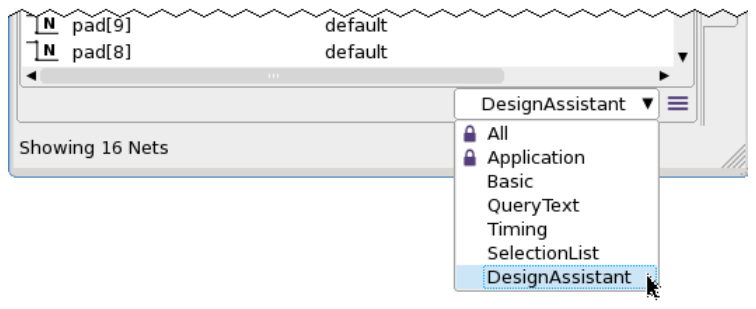
\includegraphics[width=0.92\textwidth]{gui-fig-040.png}
\caption{设计助手的属性组选择器}
\label{fig:gui-40}
\end{figure}

表中的条目可用属性组管理器（Attribute Group Manager）配置。单击对话框右下角的 Modify Attribute Group 按钮，再单击 Manage All，即可打开 Attribute Group Manager。

\begin{seeAlsoBox}
Attribute Group Manager 的用法见第~\ref{chap:gui-toolbar}~章。
\end{seeAlsoBox}

还可以对表中的列标题执行下列操作：
\begin{itemize}
  \item 单击列标题，按该列对列表中的数据排序。
  \item 再次单击该列标题，反转排序顺序。
  \item 单击列标题并把它拖到新位置，以改变列的顺序，见图~\ref{fig:gui-41}。
\end{itemize}

\begin{figure}[htbp]
\centering
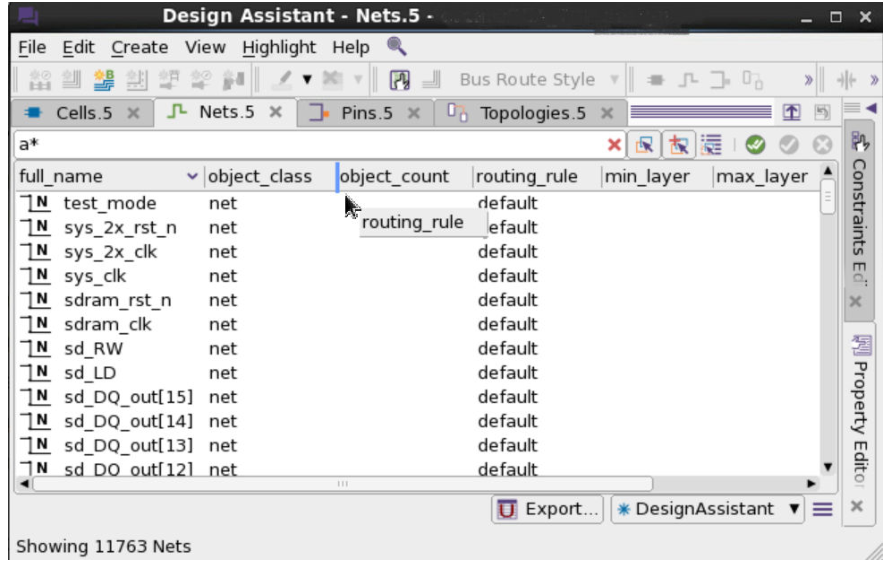
\includegraphics[width=0.92\textwidth]{gui-fig-041.png}
\caption{在设计助手中重排列}
\label{fig:gui-41}
\end{figure}

\begin{itemize}
  \item 右键单击列标题，选择 \textbf{Sort Increasing} 或 \textbf{Sort Decreasing}，对列排序。
  \item 右键单击列标题，选择 \textbf{Fit All Columns} 或 \textbf{Fit Column}，使列宽适应设计助手对话框，见图~\ref{fig:gui-42}。
\end{itemize}

\begin{figure}[htbp]
\centering
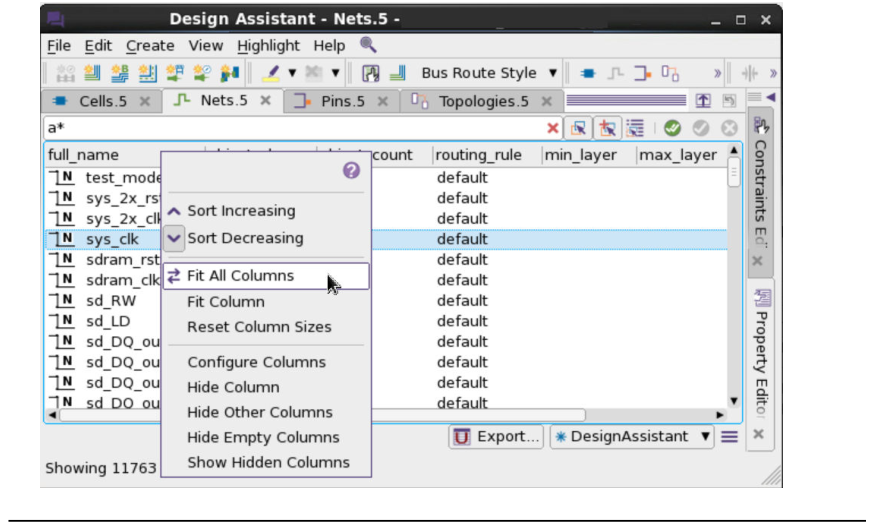
\includegraphics[width=0.92\textwidth]{gui-fig-042.png}
\caption{在设计助手中适配列宽}
\label{fig:gui-42}
\end{figure}

\subsection{更改多个对象的属性设置}
\subsubsection*{Changing Property Settings for Multiple Objects}

可以一次更改多个对象的属性设置。要更改多个所选对象的某项属性：
\begin{enumerate}
  \item 在设计助手中选择多个对象：按住 Shift 键单击表中的各行。也可以按住鼠标并拖动，以选择多行。
  \item 单击某一对象所在的行并更改其值，从而更改该单个对象的属性。
  \item 单击 Apply 按钮，把更改应用到全部所选对象。
\end{enumerate}

见图~\ref{fig:gui-43}。

\begin{figure}[htbp]
\centering
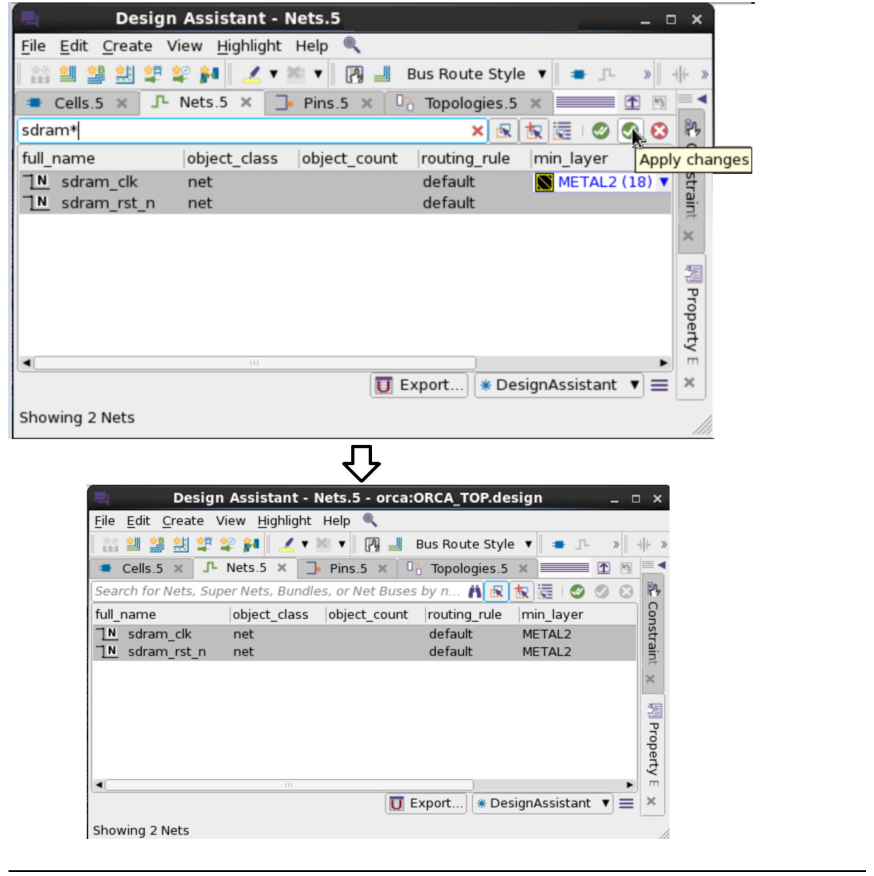
\includegraphics[width=0.92\textwidth]{gui-fig-043.png}
\caption{将更改应用到设计助手中的多个对象}
\label{fig:gui-43}
\end{figure}

\subsection{自动应用更改}
\subsubsection*{Applying the Changes Automatically}

要使更改自动应用到设计，在 Cells、Nets、Pins 和 Topologies 选项卡上单击 Auto Apply Changes，见图~\ref{fig:gui-44}。

\begin{figure}[htbp]
\centering
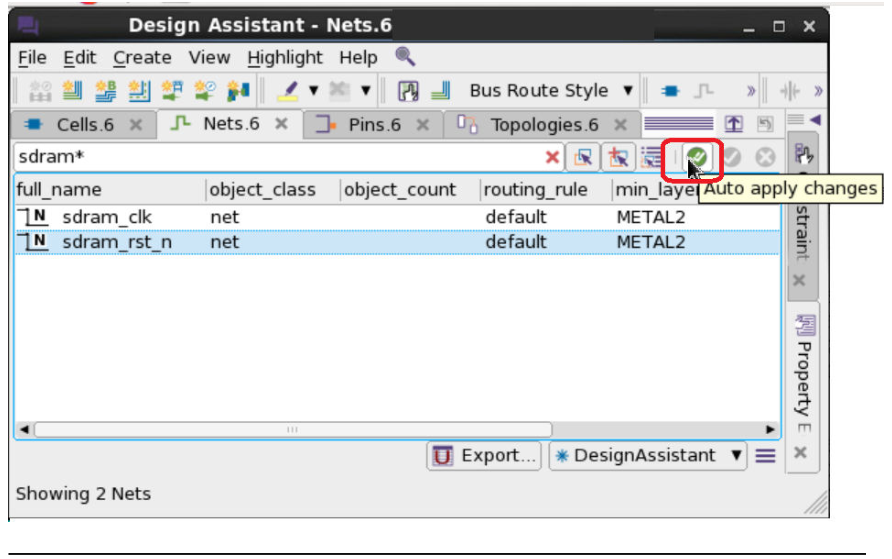
\includegraphics[width=0.92\textwidth]{gui-fig-044.png}
\caption{在设计助手中自动应用更改}
\label{fig:gui-44}
\end{figure}

\subsection{使选择与全局选择同步}
\subsubsection*{Synchronizing the Selection With the Global Selection}

在版图窗口中选择对象时，要使设计助手窗口中对应的对象或行一并被选中，在设计助手窗口的 Cells、Nets、Pins 和 Topologies 选项卡上单击 Synchronize Global Selection 按钮，见图~\ref{fig:gui-45}。

\begin{figure}[htbp]
\centering
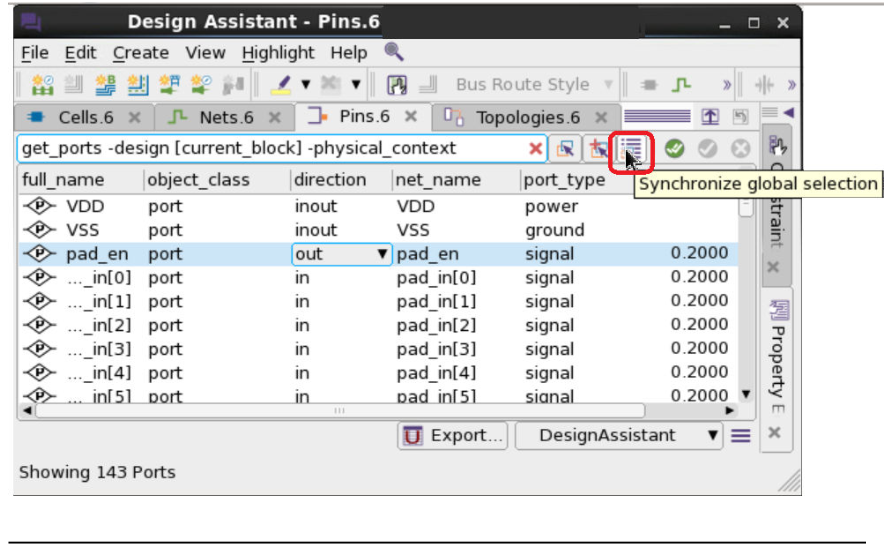
\includegraphics[width=0.92\textwidth]{gui-fig-045.png}
\caption{在设计助手中与全局选择同步}
\label{fig:gui-45}
\end{figure}

\subsection{执行相关任务}
\subsubsection*{Performing Related Tasks}

设计助手窗口中的每个选项卡都支持上下文菜单，其中列出可对对象列表执行的各项任务。把指针移到列表中的一项上，单击鼠标右键即可查看上下文菜单。上下文菜单显示与所选对象相关的任务。例如，在 Cells 选项卡中打开上下文菜单时，菜单会显示所选对象的 \textbf{Get Nets}、\textbf{Get Hierarchical Nets}、\textbf{Get Pins} 和 \textbf{Create Bounds} 任务。单击上下文菜单中的项即可执行该任务。从上下文菜单选择任务后，工具会打开相应选项卡并显示信息。另一个例子是：在 Topologies 选项卡上打开上下文菜单时，菜单会显示所选对象的 \textbf{Get Nets} 任务。要查看或隐藏拓扑规划（topology plan），分别执行 \textbf{Show Topology Plans (hierarchical)} 或 \textbf{Hide Topology Plans} 任务。

\begin{noteBox}
同样的相关操作也可以从菜单栏选择。例如，要显示 Cells 选项卡中所选项目的线网，从设计助手菜单栏选择 \textbf{Cells > Get Nets}。在设计助手中切换不同选项卡时，菜单栏中的项目会随之改变。
\end{noteBox}

也可以用上下文菜单高亮（highlight）对象、放大以查看对象、把用于选择该对象的 Tcl 命令写入脚本文件，以及执行其他任务。单击上下文菜单中的项即可执行相应操作。

\subsection{使用约束编辑器}
\subsubsection*{Using the Constraints Editor}

使用 Constraints Editor 面板显示并修改线网约束、拓扑约束和成形约束（shaping constraint）。线网约束包括与 Nets 选项卡中所选对象关联的非默认布线规则（nondefault routing rule）和布线走廊（routing corridor）。成形约束包括目标位置（target location）、父对象（parent object）、边界（boundary）、利用率（utilization）等，由 \cmd{create\_shaping\_constraint} 命令设置。拓扑约束包括与 Topologies 选项卡上所选拓扑规划关联的拓扑节点（topology node）、拓扑边（topology edge）和中继器（repeater）。

要用该面板查看并修改全部约束：
\begin{enumerate}
  \item 从设计助手菜单选择 \textbf{View > Toolbars > Constraints Editor}，或单击 Constraints Editor 选项卡。
  \item 在 Nets、Topologies 或 Shapeable 视图中选择一个对象。
  \item 单击表中的对象名。
  \item 单击约束列表中的约束类型，查看该约束的属性。
  \item （可选）在属性编辑表中修改该约束的属性。
  \item （可选）在约束表中的约束类型上右键单击，选择 \textbf{Select}、\textbf{Select Owners} 或 \textbf{Delete}，以选择或删除该约束类型。
  \item （可选）单击 Options 按钮（齿轮图标），打开 Synchronize Global Selection 模式，使全局选择与 Constraints Editor 中的选择双向同步。
\end{enumerate}

设计助手视图与 Constraints Editor 调色板（palette）中的该选项互斥，不能同时启用。

要用该面板查看并修改线网约束：
\begin{enumerate}
  \item 从设计助手菜单选择 \textbf{View > Shapeable Objects}。
  \item 从设计助手菜单选择 \textbf{View > Toolbars > Constraints Editor}，或单击 Constraints Editor 选项卡。
  \item 单击表中的对象名。
  \item 单击约束列表中的 [+] 符号，查看该约束的属性。
  \item （可选）在属性编辑表中修改该约束的属性。
  \item （可选）在约束表中的约束类型上单击鼠标右键，选择 \textbf{Select}、\textbf{Select Owners} 或 \textbf{Delete}，以选择或删除该约束类型。
\end{enumerate}

线网约束界面见图~\ref{fig:gui-46}。

\begin{figure}[htbp]
\centering
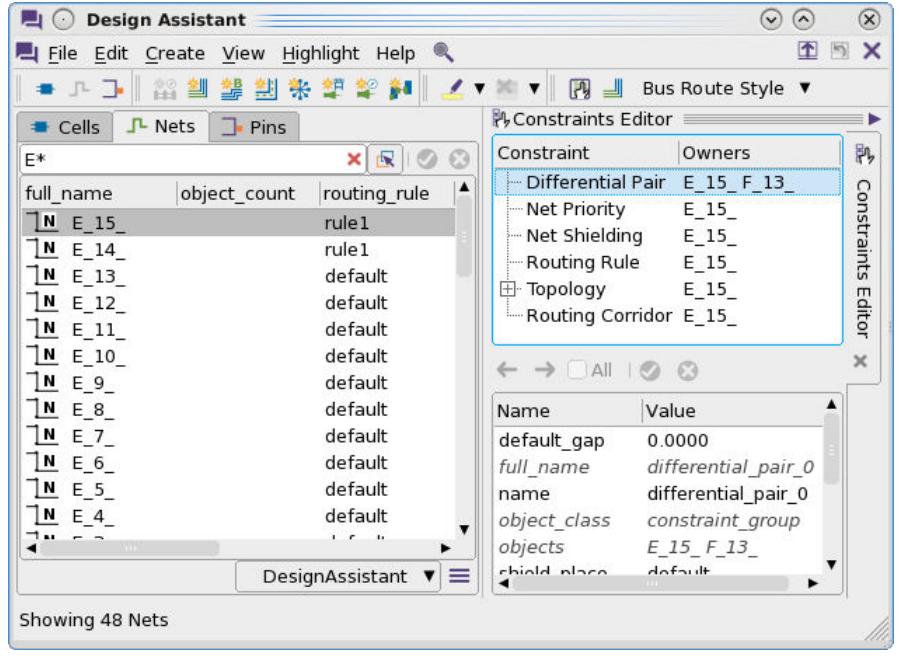
\includegraphics[width=0.92\textwidth]{gui-fig-046.png}
\caption{设计助手的线网约束}
\label{fig:gui-46}
\end{figure}

Constraints Editor 支持基于表达式的过滤和列过滤。单击一条约束并按正斜杠（/）键，即可显示过滤表达式框。也可以在列标题上单击鼠标右键，再单击 Show/Hide Filter Control 按钮，以显示过滤表达式框。在框中输入表达式并按 Enter 键，即可过滤结果。

要做列过滤，单击 Show/Hide column filter control 按钮。工具在每个列标题右侧显示漏斗图标。单击该图标即可显示列过滤菜单，见图~\ref{fig:gui-47}。

\begin{figure}[htbp]
\centering
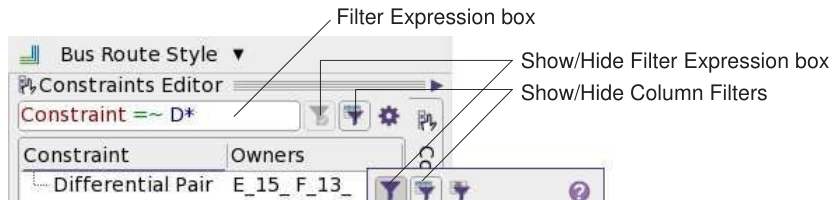
\includegraphics[width=0.92\textwidth]{gui-fig-047.png}
\caption{设计助手的列过滤}
\label{fig:gui-47}
\end{figure}

\subsection{高亮对象}
\subsubsection*{Highlighting Objects}

要在版图中高亮对象，把指针移到列表中的条目上，单击鼠标右键打开上下文菜单，再单击 \textbf{Highlight} 以高亮该对象。也可以在列表中选中对象，然后从设计助手菜单栏选择 \textbf{Highlight > Selected}。要清除某一高亮，选中该对象，并从菜单栏选择 \textbf{Highlight > Clear Selected}。选择 \textbf{Highlight > Clear All} 可清除全部高亮。

\subsection{读写对象选择脚本}
\subsubsection*{Reading and Writing Object Selection Scripts}

要把返回当前选项卡中当前所选对象列表的 Tcl 命令存盘，从菜单栏选择 \textbf{File > Write Script}，或单击鼠标右键并从上下文菜单选择 \textbf{Write Script}。

\begin{noteBox}
执行此操作时，至少要已选中一个对象。
\end{noteBox}

转到要保存文件的目录，输入文件名并单击 Save，即可写出文件。设计助手写出的脚本包含 \cmd{get\_pins}、\cmd{get\_nets} 或 \cmd{get\_cells} 命令，后接当前所选对象的名称。

要从设计助手读取 Tcl 脚本，选择 \textbf{File > Read Script}，或单击鼠标右键并从上下文菜单选择 \textbf{Read Script}。

\section{用相对位置约束工具设置约束}
\subsection*{Setting Constraints With the Relative Location Constraints Tool}

相对位置约束（relative location constraint）工具用于设置、查看和删除硬宏（hard macro）的布局约束。要启动该工具，从菜单选择 \textbf{View > Assistants > Relative Location Constraints}。Relative Location Constraints 面板出现在版图底部，见图~\ref{fig:gui-48}。列表框显示设计中的硬宏实例，以及已指定的相对位置约束。单击列标题可对表排序；再次单击则按相反顺序排序。

\begin{figure}[htbp]
\centering
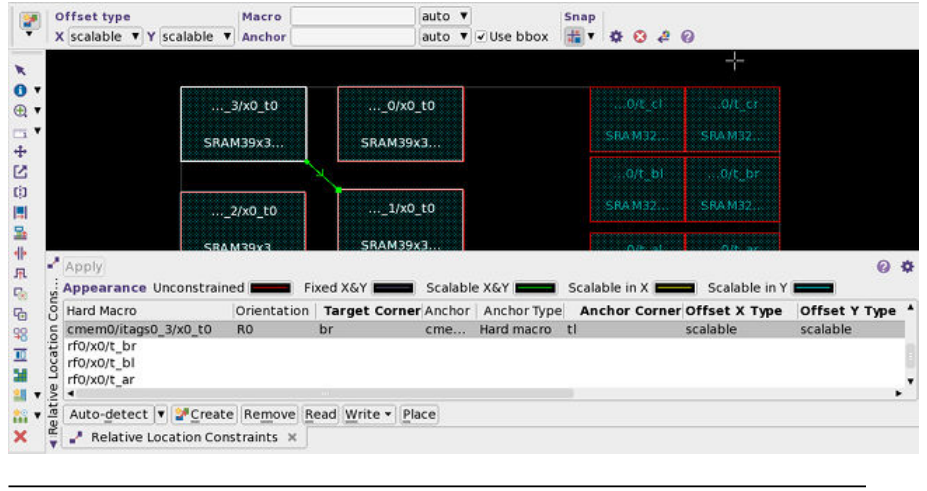
\includegraphics[width=0.92\textwidth]{gui-fig-048.png}
\caption{相对位置约束面板}
\label{fig:gui-48}
\end{figure}

\subsection{手动创建相对位置约束}
\subsubsection*{Manually Creating Relative Location Constraints}

要创建相对位置约束：
\begin{enumerate}
  \item 单击 Create 按钮，开始定义约束。
  \item （可选）按需要在 Mouse Tool Options 工具栏中更改 Offset type 及其他设置。
  \item 单击要约束的目标宏（target macro）的一角，如图~\ref{fig:gui-49} 中的 (1)。
  \item 单击锚点对象（anchor object）的一角，以定义锚点角，如图~\ref{fig:gui-49} 中的 (2)。若难以点中，请确认该锚点对象类型在 View Settings 面板中是可选的。\\
        工具在目标宏与锚点对象的角之间显示约束飞线（constraint flyline），如图~\ref{fig:gui-49} 中的 (3)；Relative Location Constraints 面板中的约束表会更新，以显示这条新约束。
  \item （可选）重复步骤 2 至 4，定义更多宏的相对位置约束。
  \item 按 Esc 退出 Create Macro Relative Location Constraint 工具。
\end{enumerate}

\begin{figure}[htbp]
\centering
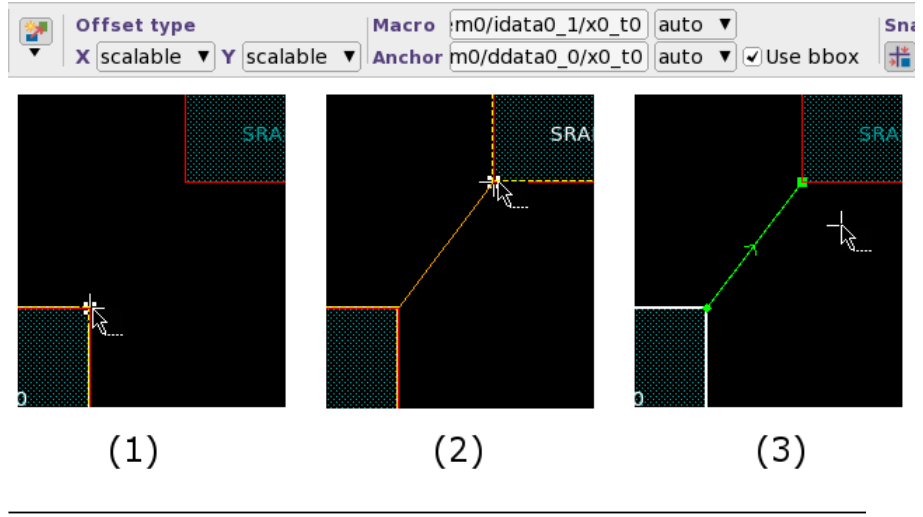
\includegraphics[width=0.92\textwidth]{gui-fig-049.png}
\caption{手动创建相对宏约束}
\label{fig:gui-49}
\end{figure}

\subsection{自动创建相对位置约束}
\subsubsection*{Automatically Creating Relative Location Constraints}

该工具支持自动创建相对位置约束。要为一组所选宏创建约束：
\begin{enumerate}
  \item 用下列方法之一选择一个或多个宏：
  \begin{itemize}
    \item 单击表中的一行。
    \item 单击表中的一行并拖动，以选择多个宏。
    \item 在表中单击，再按 Ctrl+A 选择全部宏。
    \item 在版图中单击一个或多个宏。
  \end{itemize}
  \item 单击 Auto-detect 按钮。\\
        工具为全部所选宏创建相对位置约束。
\end{enumerate}

\subsection{按相对位置约束放置宏}
\subsubsection*{Placing Macros Using Relative Location Constraints}

要按相对位置约束放置宏，单击 Place 按钮，并在出现的对话框中单击 OK。工具运行 \cmd{create\_macro\_relative\_location\_placement} 命令，根据相对位置约束更新宏的布局。

\subsection{删除相对位置约束}
\subsubsection*{Removing Relative Location Constraints}

要删除一条或多条相对位置约束：
\begin{enumerate}
  \item 选择一个或多个宏。
  \item 单击 Remove 按钮以删除约束。
\end{enumerate}

图~\ref{fig:gui-50} 是选中两个宏的约束表。在此例中，单击 Remove 按钮会删除所选宏的约束。

\begin{figure}[htbp]
\centering
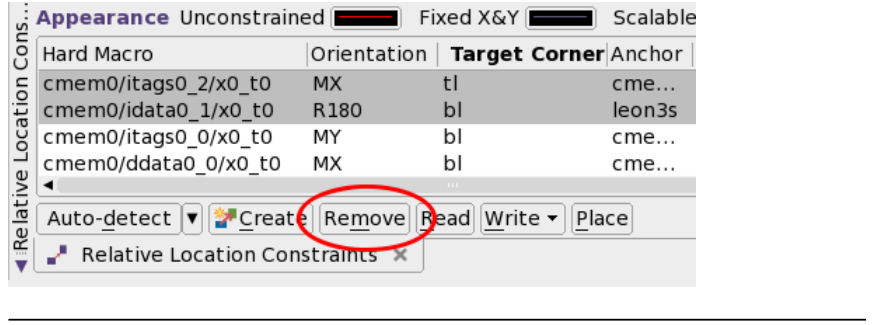
\includegraphics[width=0.92\textwidth]{gui-fig-050.png}
\caption{删除相对位置约束}
\label{fig:gui-50}
\end{figure}

\subsection{写出相对位置约束}
\subsubsection*{Writing Out Relative Location Constraints}

要把已定义约束的全部宏的相对位置约束写出，单击 Write 按钮，选择 Macro relative location，并输入用于保存约束的文件名。对于每个已定义宏相对约束的宏，工具写出一条 \cmd{set\_macro\_relative\_location} 命令。下列示例给出两条已定义的约束：

\begin{lstlisting}
# macro_relative_constraints.tcl
set_macro_relative_location \
   -target_object [get_cells u1/REG_FILE_D_RAM] \
   -target_orientation R0 -target_corner tr \
   -anchor_object [get_blocks ORCA] -anchor_corner tr -offset { \
   -0.1594 -0.2488} -offset_type scalable \
   -used_length {0.0000 0.0000} -scale_edge {0 0}

set_macro_relative_location \
   -target_object [get_cells u2/SD_FIFO_RAM] \
   -target_orientation MXR90 -target_corner br \
   -anchor_object [get_blocks ORCA] -anchor_corner br -offset { \
   -0.1715 0.2576} -offset_type scalable \
   -used_length {0.0000 0.0000} -scale_edge {0 0}

set_attribute -objects [get_blocks test:ORCA.design] \
   -name edge_number -value 4 -quiet
\end{lstlisting}

\subsection{写出端口相对位置约束}
\subsubsection*{Writing Out Port Relative Location Constraints}

要把全部 I/O 端口（I/O port）的端口相对位置约束写出，单击 Write 按钮，选择 Port relative location，并输入用于保存约束的文件名。对于每个已定义相对约束的 I/O 端口，工具写出一条 \cmd{set\_individual\_pin\_constraints} 命令。含有两条已定义约束的设计，其示例文件如下：

\begin{lstlisting}
# Port relative location constraints
# Generated on Feb 3 12:51:21
...
set_individual_pin_constraints -ports [get_ports pad[15]] \
   -sides 2 -offset [mrl_get_offset 2 0.5]
set_individual_pin_constraints -ports [get_ports pad[14]] \
   -sides 2 -offset [mrl_get_offset 2 0.5]
...
\end{lstlisting}

\subsection{读入相对位置约束}
\subsubsection*{Reading In Relative Location Constraints}

要读入宏或 I/O 端口的相对位置约束，单击 Read 按钮，并输入包含宏相对位置约束或 I/O 端口相对位置约束的脚本文件名。工具读取该文件并应用约束。

\subsection{更改约束飞线的颜色}
\subsubsection*{Changing the Color of the Constraint Flylines}

定义了宏相对约束后，工具在宏与对象之间显示约束飞线。要更改约束飞线的颜色：
\begin{enumerate}
  \item 单击面板顶部附近 Appearance 区中的一条色条。
  \item 在 Select Style 对话框中选择新颜色，并单击 OK。
  \item 单击 Apply 以应用更改。
\end{enumerate}

工具用新颜色重新显示约束飞线。

\section{使用网表追踪器}
\subsection*{Using the Netlist Tracer}

IC Compiler II 工具提供网表追踪器（Netlist Tracer），用于追踪一条线网在设计中的路径。从菜单选择 \textbf{View > Assistants > Netlist Tracer} 即可启动网表追踪器。用网表追踪器沿设计遍历线网路径。先选择作为追踪起点的单元、线网、管脚或端口。可以遍历连接到该对象的线网路径，高亮该路径，并放大相关的单元、线网和管脚。追踪路径时，网表追踪器在当前对象与任何相连对象之间显示飞线（flyline）。界面见图~\ref{fig:gui-51}。

\begin{figure}[htbp]
\centering
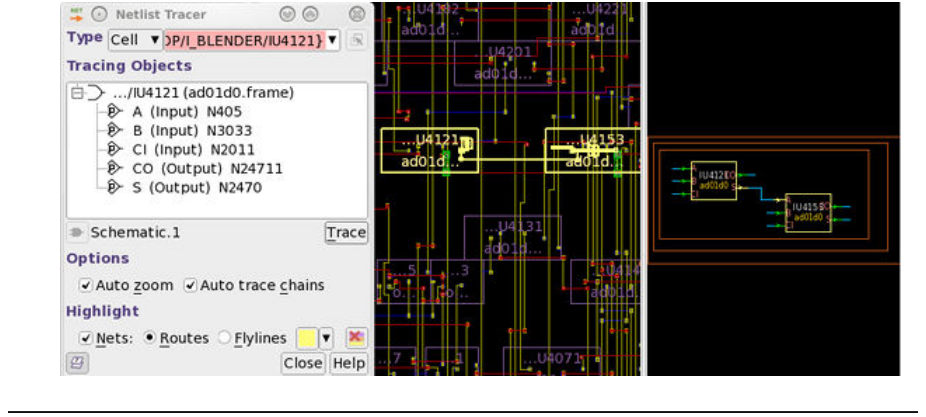
\includegraphics[width=0.92\textwidth]{gui-fig-051.png}
\caption{网表追踪器}
\label{fig:gui-51}
\end{figure}

\section{使用布线轨道助手}
\subsection*{Using the Track Assistant}

用 Track Assistant 面板检查当前设计中的布线轨道（routing track）。布线轨道助手显示所选布线层上轨道的包围盒（bounding box），并显示轨道编号（track number），以表示轨道相对所选区域的位置。可以按层、宽度、首选方向（preferred direction）与非首选方向（nonpreferred direction）以及障碍（obstruction）显示轨道。

要启动布线轨道助手，从菜单选择 \textbf{View > Assistants > Track Assistant}，或单击 Track Assistant 按钮。以下几节说明如何使用布线轨道助手。面板见图~\ref{fig:gui-52}。

\begin{figure}[htbp]
\centering
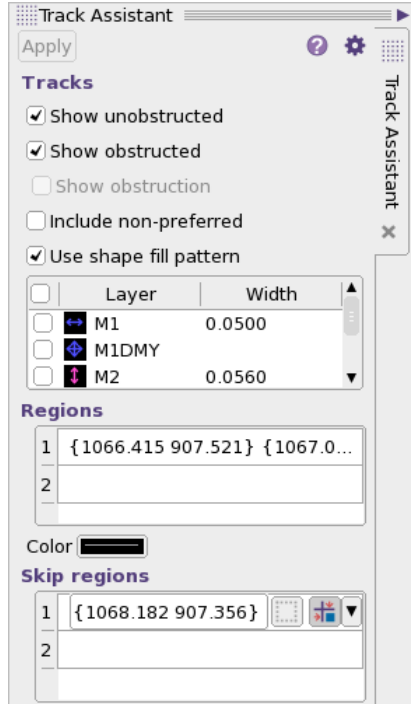
\includegraphics[width=0.92\textwidth]{gui-fig-052.png}
\caption{布线轨道助手}
\label{fig:gui-52}
\end{figure}

\subsection{显示轨道}
\subsubsection*{Displaying Tracks}

要用布线轨道助手显示轨道：
\begin{enumerate}
  \item 从菜单选择 \textbf{View > Assistants > Track Assistant}，启动布线轨道助手。
  \item 放大到要检查的版图区域。
  \item 选择要显示轨道的层。\\
        工具按所选层的轨道宽度显示布线轨道，见图~\ref{fig:gui-53}。默认情况下，工具同时显示畅通轨道与受阻轨道。
\end{enumerate}

\begin{figure}[htbp]
\centering
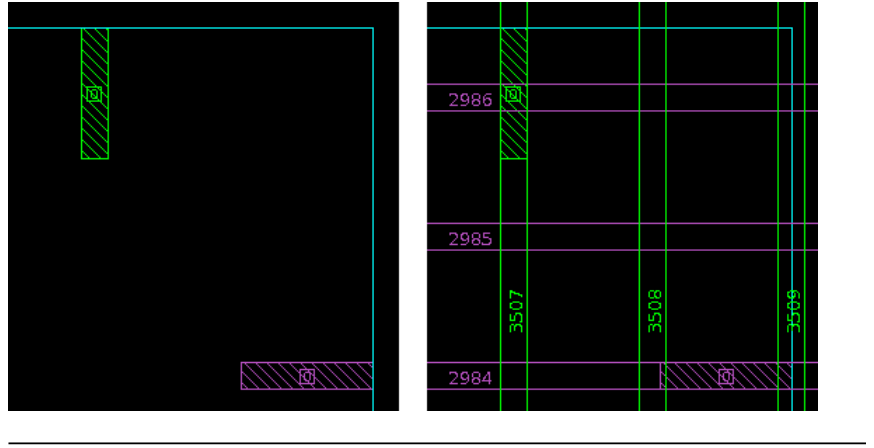
\includegraphics[width=0.92\textwidth]{gui-fig-053.png}
\caption{显示轨道之前与之后}
\label{fig:gui-53}
\end{figure}

\subsection{在指定区域显示轨道信息}
\subsubsection*{Displaying Track Information in Specific Regions}

用布线轨道助手中的选项，可以把轨道显示限制在设计的指定区域。要只显示设计中某些区域的轨道信息：
\begin{enumerate}
  \item 按上一节所述启动布线轨道助手并选择层。
  \item 在 Regions 区的空行中单击，并输入要显示区域的包围盒。\\
        也可以单击 Specify Rectangle 按钮，在版图上画出该区域。要清除区域，把鼠标指针移到面板中的包围盒坐标上，并单击 Clear region 按钮。
  \item （可选）按需要重复上一步，画出更多区域。
  \item （可选）在 Skip regions 区的空行中单击，并输入该区域的包围盒，以创建一个隐藏轨道显示的区域。\\
        也可以单击 Specify Rectangle 按钮，在版图上画出跳过区域（skip region）。
\end{enumerate}

图~\ref{fig:gui-54} 是版图与布线轨道助手面板，其中只显示一个指定区域以及一个跳过区域。

\begin{noteBox}
已定义区域之外不显示轨道。
\end{noteBox}

\begin{figure}[htbp]
\centering
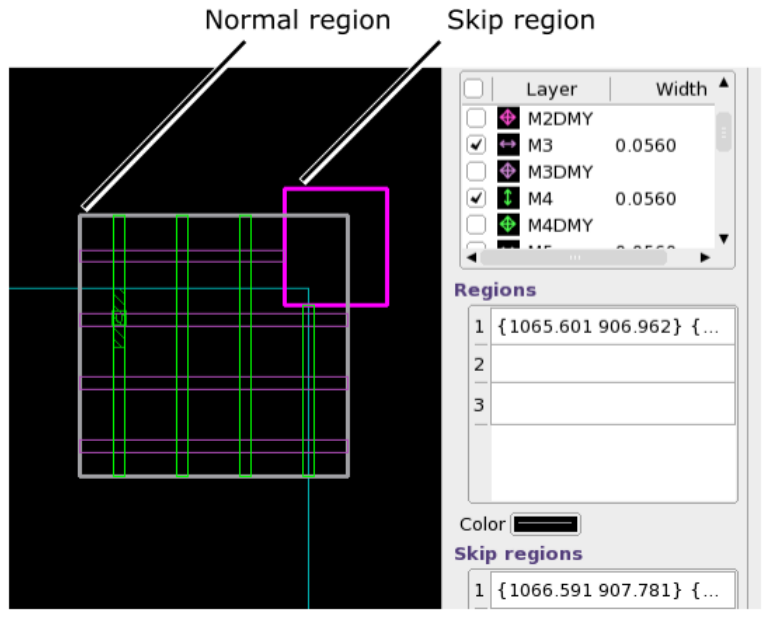
\includegraphics[width=0.92\textwidth]{gui-fig-054.png}
\caption{带普通区域与跳过区域的布线轨道助手}
\label{fig:gui-54}
\end{figure}

\subsection{显示受阻或畅通的轨道}
\subsubsection*{Displaying Obstructed or Unobstructed Tracks}

启动布线轨道助手时，工具同时显示受阻轨道（obstructed track）与畅通轨道（unobstructed track）。要只显示畅通轨道，选中 Show unobstructed 选项，并取消选中 Show obstructed 选项。要只显示受阻轨道，取消选中 Show unobstructed 选项，并选中 Show obstructed 选项。要高亮障碍，选中 Show obstruction 选项。

图~\ref{fig:gui-55} 是显示受阻轨道时的面板设置与版图。

\begin{figure}[htbp]
\centering
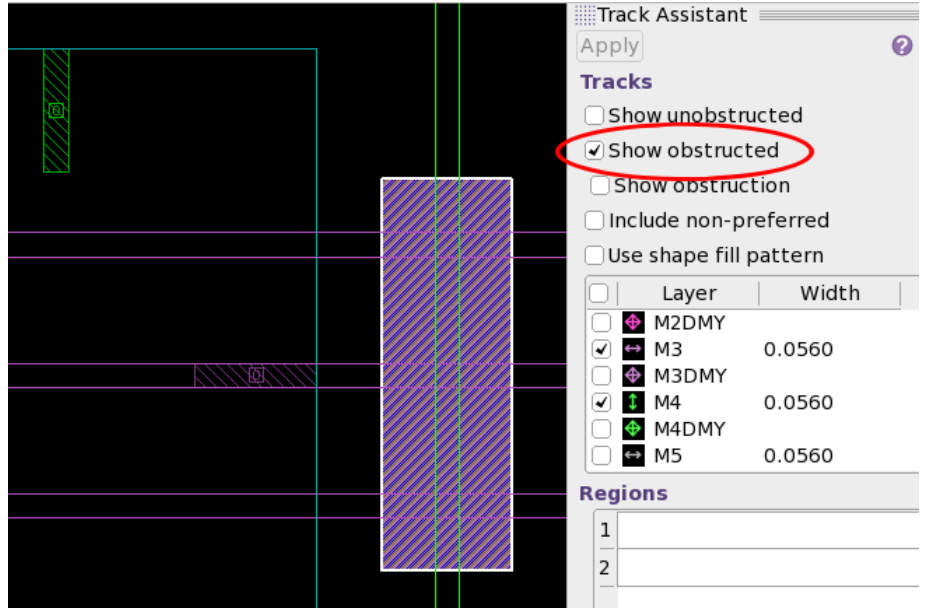
\includegraphics[width=0.92\textwidth]{gui-fig-055.png}
\caption{受阻轨道}
\label{fig:gui-55}
\end{figure}

\subsection{设置布线轨道助手选项}
\subsubsection*{Setting Track Assistant Options}

Track Assistant 面板还支持下列选项：
\begin{itemize}
  \item 选择 Include non-preferred 选项，同时显示首选布线方向与非首选布线方向上的轨道。
  \item 选择 Use shape fill pattern 选项，使布线轨道使用与金属层相同的填充图案。
  \item 单击区域列表下方的色条，并在 Select Style 对话框中选择新颜色，以设置普通区域或跳过区域的颜色。
\end{itemize}

% 第 4 章 Using Design Planning Tools
\bichapter{使用设计规划工具}{Using Design Planning Tools}
\label{chap:gui-dp}

IC Compiler II GUI 提供支持设计规划（design planning）中各项任务的工具。假设通道拥塞（What-if Channel Congestion）工具支持交互式假设分析（what-if analysis），用来找出拥塞的全局布线通道。层次探索（Hierarchy Exploration）工具支持与模块边界（module boundary）相关的若干任务。

下列主题说明 GUI 所支持的设计规划任务：
\begin{itemize}
  \item 层次浏览器
  \item 基于名称的层次浏览器
  \item 假设通道拥塞
  \item 层次探索
  \item 拓扑管脚约束
  \item 使用管脚约束
  \item 执行拓扑互连规划
\end{itemize}

\section{层次浏览器}
\subsection*{Hierarchy Browser}

本工具提供用于探索设计层次的工具，以便确定要把哪些逻辑层次单元提交（commit）为物理层次块。GUI 中的层次浏览器（Hierarchy Browser）显示设计层次，并提供每个层次单元的其他信息。

用 Hierarchy Browser 探索设计层次：
\begin{enumerate}
  \item 在 GUI 中选择 \textbf{View > Hierarchy Browser}。
  \item 单击层次单元旁的 [+] 符号，展开或折叠层次。
  \item 单击列标题，重排显示。
  \item 单击块名，对该块执行其他操作。
\end{enumerate}

Hierarchy Browser 中显示的层次示例如图~\ref{fig:gui-56} 所示。

\begin{figure}[htbp]
\centering
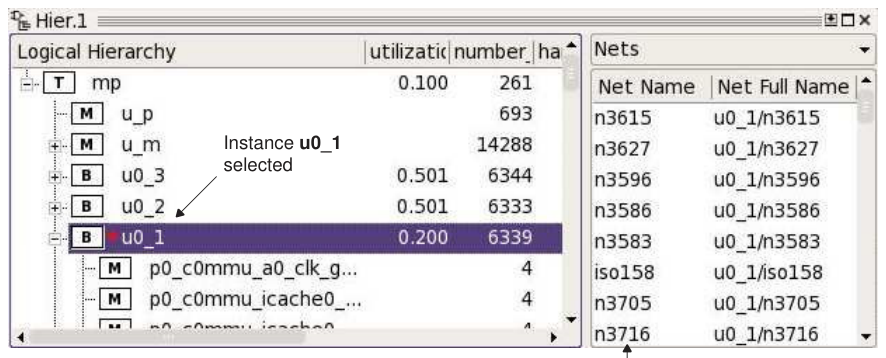
\includegraphics[width=0.92\textwidth]{gui-fig-056.png}
\caption{层次浏览器}
\label{fig:gui-56}
\end{figure}

在 Hierarchy Tree 视图中使用上下文菜单时，在逻辑层次上右键单击即可打开菜单，并执行下列操作：
\begin{itemize}
  \item 选择 \textbf{Partitioning > Create Module Boundary}，为指定层次级别创建模块边界。
  \item 选择 \textbf{Partitioning > Create Bound}，创建模块边界，并在版图窗口中启动 Create Bound 工具。在版图窗口中画出约束（bound），以完成该任务。
  \item 选择 \textbf{Partitioning > Copy Macro Relative Placement}，把硬宏（hard macro）的相对布局复制到所选模块。
  \item 选择 \textbf{Color by Hierarchy > Set Selected Color}，再从菜单中选择一种颜色，改为指定颜色。
  \item 选择 Commit Block，把逻辑层次单元提交为物理层次块。
  \item 选择 Clear Selection，取消层次中全部已选对象的选择。
  \item 选择 Select Related Objects，再从列表中选择一项，以选择与该对象关联的连接、宏、安全核规则（safety core rule）、安全核组（safety core group）等。
\end{itemize}

也可以从下列位置之一查看相关对象：
\begin{itemize}
  \item 版图视图（Layout view）
  \item Select 菜单：
  \begin{itemize}
    \item \textbf{Select > By Name Toolbar}，或
    \item \textbf{Select > By Name}，或
    \item \textbf{Select > Related Objects}，或
  \end{itemize}
  \item 上下文相关菜单（右键单击对象，再选择 \textbf{Select Related Objects}）
\end{itemize}

例如，选中一条拓扑边（topology edge）或一个拓扑规划（topology plan）时，上下文菜单会随之显示。

使用 Selection List 面板、Properties 面板或 Queries 面板，查看所选对象的更多细节。
\begin{itemize}
  \item 选择 Properties，打开对话框，显示所选逻辑层次的属性。
  \item 选择 Expand Tree，显示所选逻辑层次的子层次。
  \item 选择 Copy Text，复制所选单元的名称。复制的文本同时进入复制缓冲区（copy buffer）和剪贴板。
\end{itemize}

可从 Hierarchy Tree 视图和 Child List 视图使用该功能。
\begin{itemize}
  \item 选择 Find Copied Cell Text，搜索已复制的单元，并在 Hierarchy Tree 视图中选中它。
\end{itemize}

只有用 Copy Text 功能复制过单元名之后，才能使用该功能。
\begin{itemize}
  \item 选择 \textbf{Set Hierarchy Root > Set Root to Current Selected Cell}，更改层次树的根，并对所选对象执行操作。
\end{itemize}

在列标题上右键单击可打开上下文菜单。可以在 Child List 视图的上下文菜单中执行下列操作。

\begin{noteBox}
上下文菜单只对特定标题可用。
\end{noteBox}

\begin{itemize}
  \item 选择 Compress Bus Objects (User Table)，把带总线记法（bus notation）的对象导出到用户表（User Table），并把全部公共对象名压缩为单个总线对象（bused object）。
  \item 使用已压缩 User Table 上下文菜单中的过滤选项，查看总线对象、总线内容，或返回完整的总线表。
\end{itemize}

可以在 TreeMap 视图中执行下列操作：

在 Hier Std Color 对话框上选择 Outliers，高亮设计中落在指定最小值与最大值范围之外的那些单元。

\subsection{在层次浏览器中过滤信息}
\subsubsection*{Filtering Information in the Hierarchy Browser}
\label{sec:gui-dp-filter}

层次浏览器支持列过滤，并用过滤框过滤表中的信息。要显示过滤表达式框，执行下列操作之一：
\begin{itemize}
  \item 按正斜杠键（/），或
  \item 在列标题上右键单击，打开过滤选项。
\end{itemize}

\begin{figure}[htbp]
\centering
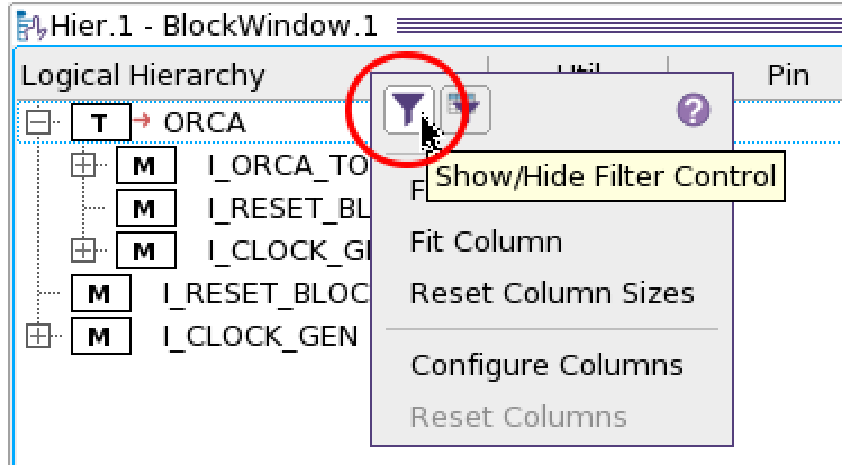
\includegraphics[width=0.92\textwidth]{gui-fig-057.png}
\caption{启用过滤}
\label{fig:gui-57}
\end{figure}

在表达式框中输入表达式，只显示与该表达式匹配的条目。

\begin{figure}[htbp]
\centering
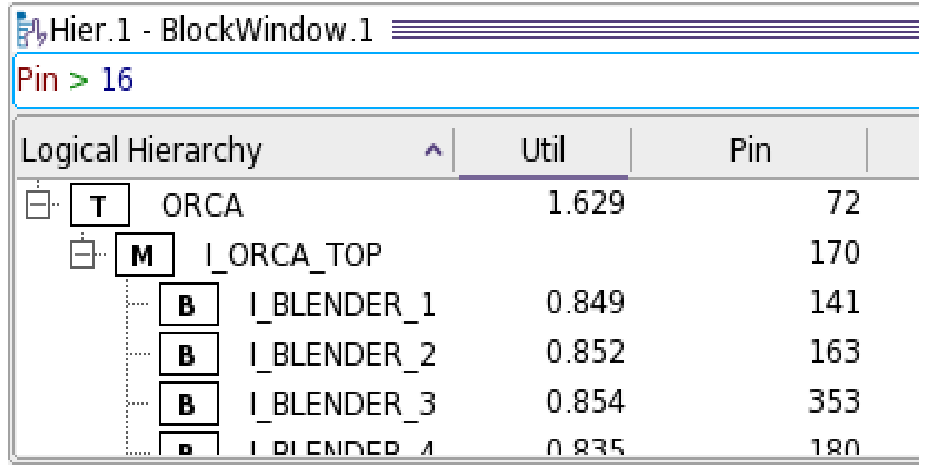
\includegraphics[width=0.92\textwidth]{gui-fig-058.png}
\caption{过滤表达式}
\label{fig:gui-58}
\end{figure}

要启用列过滤，单击过滤框右侧的 Show/Hide Column filter 控件按钮。也可以在列标题上单击鼠标右键，再单击上下文菜单中的按钮，如图~\ref{fig:gui-59} 所示。

\begin{figure}[htbp]
\centering
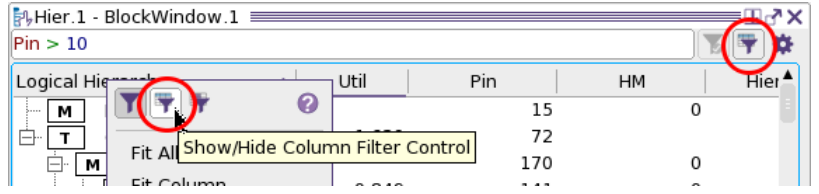
\includegraphics[width=0.92\textwidth]{gui-fig-059.png}
\caption{启用列过滤}
\label{fig:gui-59}
\end{figure}

要查看 Column Filter 菜单，单击漏斗图标。用菜单中的选项按升序或降序排列该列、创建过滤条件，或通过选择列中的特定值来过滤该列。过滤菜单如图~\ref{fig:gui-60} 所示。

\begin{figure}[htbp]
\centering
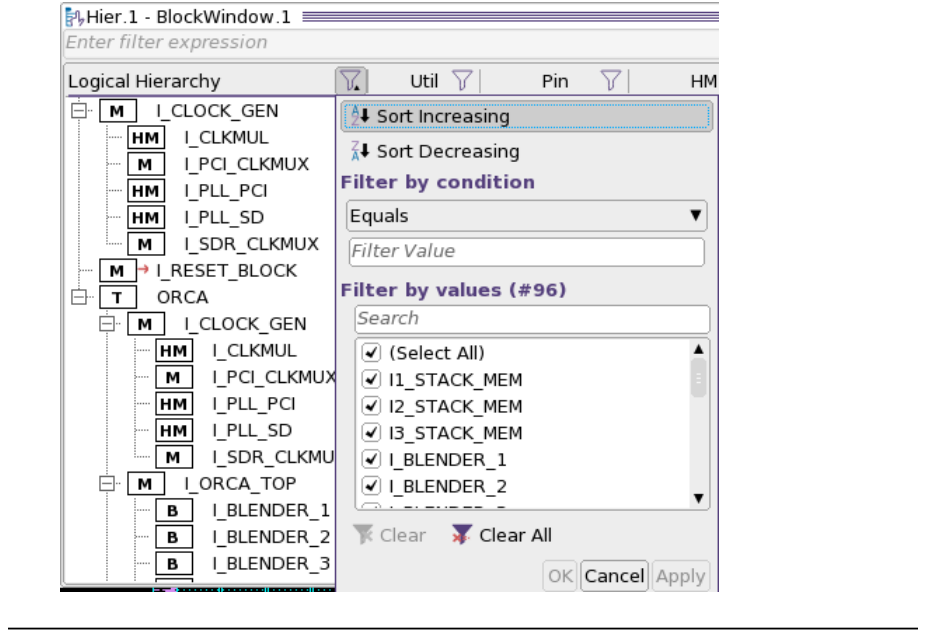
\includegraphics[width=0.92\textwidth]{gui-fig-060.png}
\caption{列过滤菜单}
\label{fig:gui-60}
\end{figure}

\section{基于名称的层次浏览器}
\subsection*{Name Based Hierarchy Browser}

对于扁平设计（flat design），本工具提供基于名称的层次浏览器（Name Based Hierarchy Browser），用来显示设计中的隐含层次（implicit hierarchy），并允许对层次执行操作。

要启动 Name Based Hierarchy Browser，选择 \textbf{View > Name Based Hierarchy Browser}。工具按图~\ref{fig:gui-61} 所示显示该浏览器。若设计含有层次，该选择被禁用，不能使用此功能。

\begin{figure}[htbp]
\centering
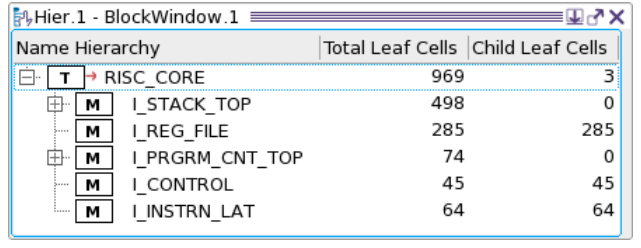
\includegraphics[width=0.92\textwidth]{gui-fig-061.png}
\caption{基于名称的层次浏览器}
\label{fig:gui-61}
\end{figure}

工具根据应用选项 \appopt{gui.name\_based\_hier\_delimiter} 的设置提取层次。默认值为「/」。可以用 \cmd{ungroup\_cells -all -flatten} 命令把设计转换为扁平设计。

与 Hierarchy Browser 类似，可以用上下文菜单执行不同操作；在层次上右键单击即可显示上下文菜单：
\begin{itemize}
  \item 选择 Set Colors On Top Hierarchies，为每个顶层层次指定一种颜色
  \item 选择 Clear All Hierarchy Colors，去掉层次上的全部颜色
  \item 选择 Set Selected Hierarchy Color 并选择一种颜色，为所选层次指定颜色
  \item 选择 Clear Selected Hierarchy Color，去掉当前所选层次的颜色
  \item 选择 Show Child List，拆分对话框并显示所选层次中的单元列表
  \item 选择 Expand All Hierarchy Trees 并选择层数，显示全部顶层层次的子层次
  \item 选择 Expand Selected Hierarchy Trees 并选择层数，显示所选层次的子层次
  \item 选择 Copy Hierarchy Path，把当前层次的实例路径复制到剪贴板
\end{itemize}

\begin{seeAlsoBox}
表中结果的过滤方法，见第~\ref{sec:gui-dp-filter}~节。
\end{seeAlsoBox}

\section{假设通道拥塞}
\subsection*{What-if Channel Congestion}

IC Compiler II 工具支持交互式假设分析，用来找出拥塞的全局布线（global routing）通道（channel）。要在版图窗口中打开 What-if Channel Congestion 图模式，在 Task Assistant 的 Design Planning 区中选择 What-if Channel Congestion，或选择 \textbf{View > Map > What-if Channel Congestion}。What-if Channel Congestion 图模式出现在版图窗口右侧，如图~\ref{fig:gui-62} 所示。

\begin{figure}[htbp]
\centering
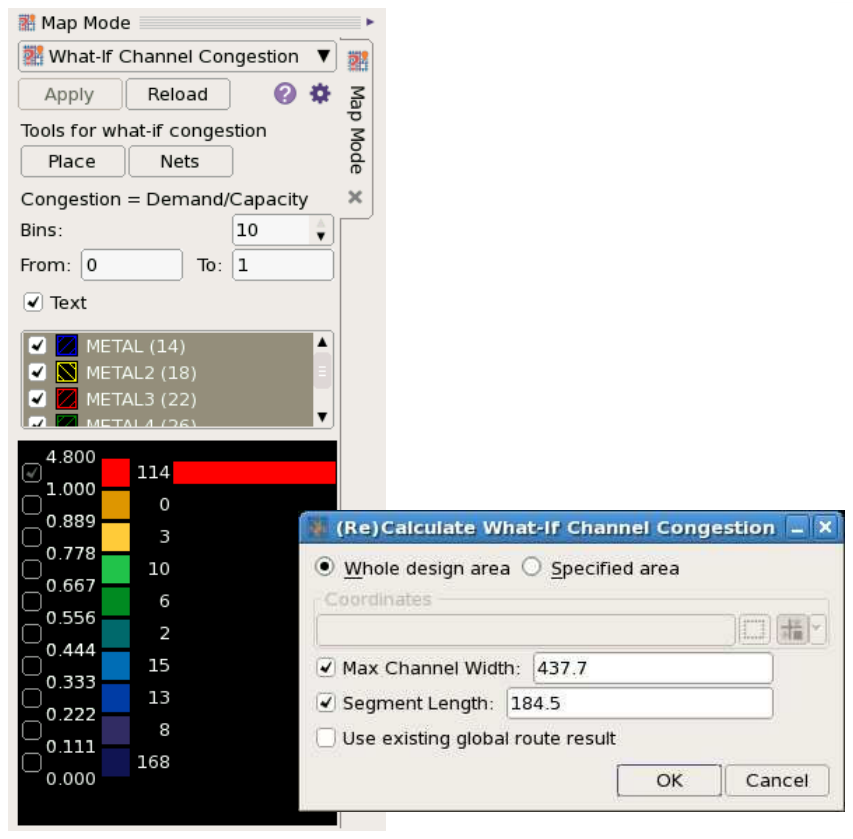
\includegraphics[width=0.92\textwidth]{gui-fig-062.png}
\caption{假设通道拥塞图模式与 Reload 对话框}
\label{fig:gui-62}
\end{figure}

\subsection{为假设通道拥塞执行全局布线}
\subsubsection*{Performing Global Routing for What-if Channel Congestion}

开始假设拥塞分析：
\begin{enumerate}
  \item 单击 Reload 按钮，打开 Calculate What-If Channel Congestion Map Data 对话框。
  \item 选择 Whole design area 或 Specified area，确定要评估的设计区域。
  \item （可选）更改 Max Channel Width 框中的值，设置要显示的最大通道尺寸；按通道宽度过滤的更多说明，见第~\ref{sec:gui-dp-chan-min}~节。
  \item （可选）更改 Segment Length；关于段长度的更多说明，见第~\ref{sec:gui-dp-chan-seg}~节。
  \item （可选）选择 Use existing global route result，使用来自 \cmd{route\_global -congestion\_map\_only true} 命令的已有布线信息。
\end{enumerate}

可以用 \cmd{remove\_routes -global\_route} 命令从设计中删除全局布线。
\begin{enumerate}
  \setcounter{enumi}{5}
  \item 单击 OK，创建拥塞图（congestion map）。
\end{enumerate}

\subsection{查看拥塞信息}
\subsubsection*{Viewing Congestion Information}

全局布线完成后，工具高亮设计中每条拥塞通道。要显示该通道的更多信息，把指针移到通道上并查看信息提示（infotip）。信息提示显示该通道以及通道内沿优选布线方向（preferred routing direction）每一层金属的需求（demand）与容量（capacity）。图~\ref{fig:gui-63} 是一条拥塞通道的信息提示。

\begin{figure}[htbp]
\centering
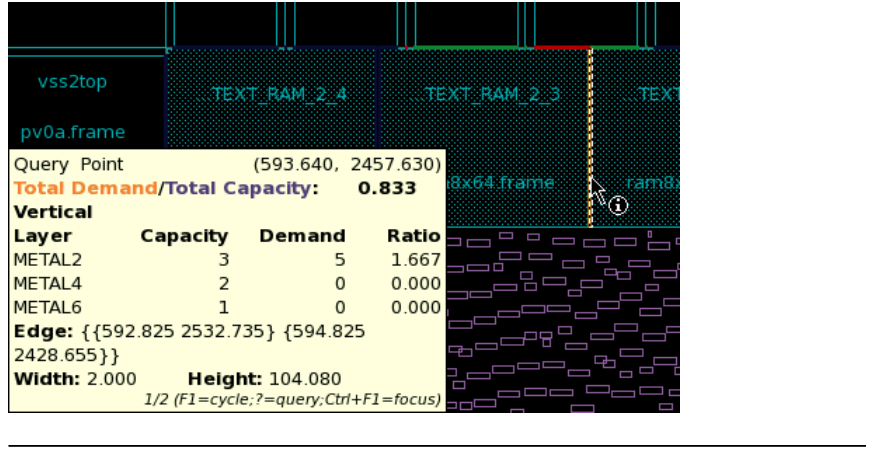
\includegraphics[width=0.92\textwidth]{gui-fig-063.png}
\caption{假设通道拥塞信息提示}
\label{fig:gui-63}
\end{figure}

\subsection{按最小通道尺寸过滤}
\subsubsection*{Filtering by Minimum Channel Dimension}
\label{sec:gui-dp-chan-min}

要只显示设计中的窄通道，单击 Reload 按钮，在 Max channel width 框中输入通道宽度值，再单击 OK。工具更新显示，并隐藏最小尺寸（高度或宽度）大于指定最大通道宽度值的通道，如图~\ref{fig:gui-64} 所示。

\begin{figure}[htbp]
\centering
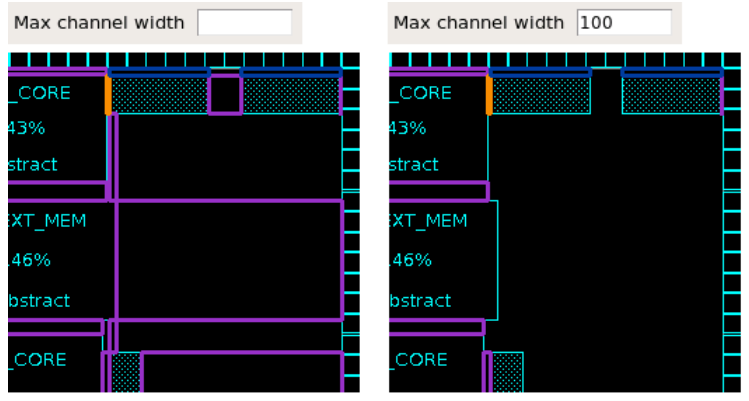
\includegraphics[width=0.92\textwidth]{gui-fig-064.png}
\caption{按最小通道尺寸过滤}
\label{fig:gui-64}
\end{figure}

\subsection{显示通道段}
\subsubsection*{Displaying Channel Segments}
\label{sec:gui-dp-chan-seg}

要做更细致的分析并把通道划分成更小的段（segment），在 Segment length 框中输入一个值。工具细分每条通道，并创建指定长度的段，如图~\ref{fig:gui-65} 所示。沿通道移动指针，在信息提示中查看每个通道段的详细拥塞信息。

\begin{figure}[htbp]
\centering
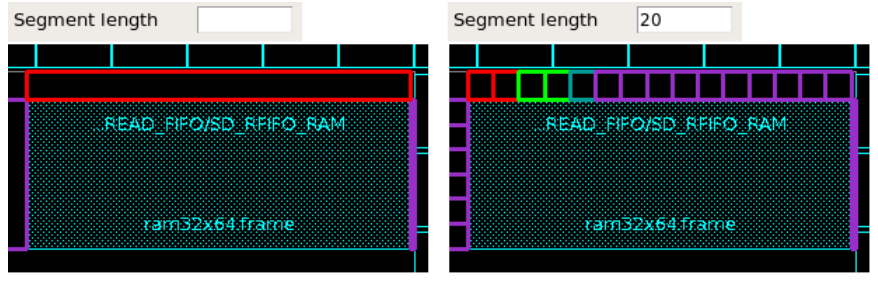
\includegraphics[width=0.92\textwidth]{gui-fig-065.png}
\caption{带分段的通道}
\label{fig:gui-65}
\end{figure}

请注意，段尺寸可能与指定值并不完全一致。某些情况下，工具会增大或缩小线段，以形成尺寸一致的段。

\subsection{指定分析区域}
\subsubsection*{Specifying the Region for Analysis}

默认情况下，工具为整个设计生成假设拥塞图。可以指定一个区域来限制分析，从而加快拥塞分析。单击 Region 框右侧的按钮，在版图窗口中画一个矩形，再单击 Apply，把分析限制在所画区域。也可以在 Region 框中指定包围盒（bounding box）的坐标，再单击 OK，只分析指定区域。

\subsection{缩放拥塞颜色映射}
\subsubsection*{Scaling the Congestion Color Mapping}

工具根据通道中所需布线数与可用布线数之比，为每条通道着色。默认情况下，比值超过 1.0（所需布线数超过可用布线数）的通道着红色，比值小于 0.2 的通道着紫色。

要更改通道的着色方式，在 From: 与 To: 框中输入值，再单击 Apply。工具重新显示拥塞图，并按这些值给通道着色。

\subsection{修正拥塞问题}
\subsubsection*{Correcting Congestion Problems}

要用 What-if Channel Congestion 分析以交互方式减轻布线拥塞，执行下列操作：
\begin{enumerate}
  \item 选择与拥塞区域邻接的硬宏
  \item 按 M，或从工具栏选择 Move 工具
  \item 用鼠标移动硬宏，在拥塞区域形成更宽的通道
\end{enumerate}

也可以按 Tab 键，在 Move 工具栏的 Delta 框中输入 x 与 y 偏移，再按 Enter。工具按指定距离移动硬宏。把硬宏移到新位置后，工具根据更新后的布局重新显示拥塞图。

重复这些步骤，直到对拥塞图和布局满意。修复前后的版图如图~\ref{fig:gui-66} 所示。

\begin{figure}[htbp]
\centering
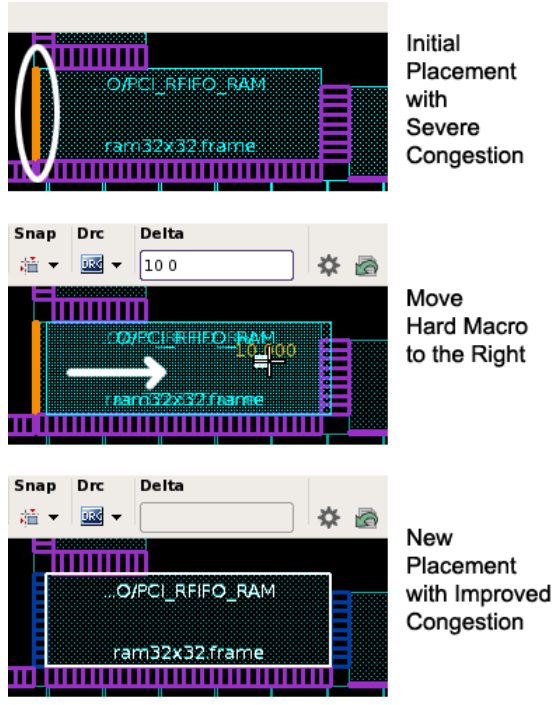
\includegraphics[width=0.92\textwidth]{gui-fig-066.png}
\caption{假设拥塞修复}
\label{fig:gui-66}
\end{figure}

\subsection{更新布局}
\subsubsection*{Updating the Placement}

调整通道宽度后，单击 Place 按钮更新单元布局。工具运行 \cmd{create\_placement -floorplan -effort medium} 命令更新布局，同时使单元保持在原先位置附近。

\subsection{显示通道中的线网}
\subsubsection*{Showing Nets in a Channel}

要显示占用某条特定通道的线网连接，单击 Nets 按钮，再在通道中单击。工具显示穿过该通道的线网，以及它们在通道外的路径。图~\ref{fig:gui-67} 是显示穿过通道的线网之前与之后的版图。要清除显示，在通道外任意位置单击。

\begin{figure}[htbp]
\centering
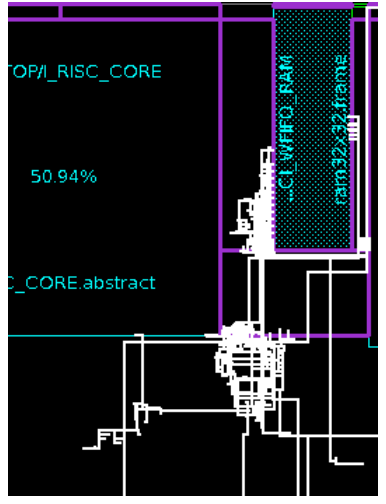
\includegraphics[width=0.92\textwidth]{gui-fig-067.png}
\caption{显示通道中的线网}
\label{fig:gui-67}
\end{figure}

\subsection{去掉拥塞图}
\subsubsection*{Removing the Congestion Map}

要从版图中去掉 What-if Channel Congestion 图，关闭 What-If Channel Congestion 图模式面板。

\section{层次探索}
\subsection*{Hierarchy Exploration}

在 IC Compiler II 工具中，模块边界表示逻辑层次中尚未提交的块。利用模块边界，可以快速评估顶层块在给定利用率（utilization）下大约需要的块尺寸，并在平面规划（floorplan）内排列模块边界，以便粗略估计块的布局。

要在版图窗口中打开 Hierarchy Exploration 面板，在 Task Assistant 的 Design Planning 区中选择 Hierarchy Exploration，或在 GUI 中选择 \textbf{View > Assistants > Hierarchy Exploration}。Hierarchy Exploration 面板出现在版图窗口右侧。

\subsection{创建模块边界}
\subsubsection*{Creating Module Boundaries}

要创建模块边界，单击 Hierarchy Exploration 面板中的 Initialize 按钮。工具为顶层模块插入模块边界，如图~\ref{fig:gui-68} 所示。

\begin{figure}[htbp]
\centering
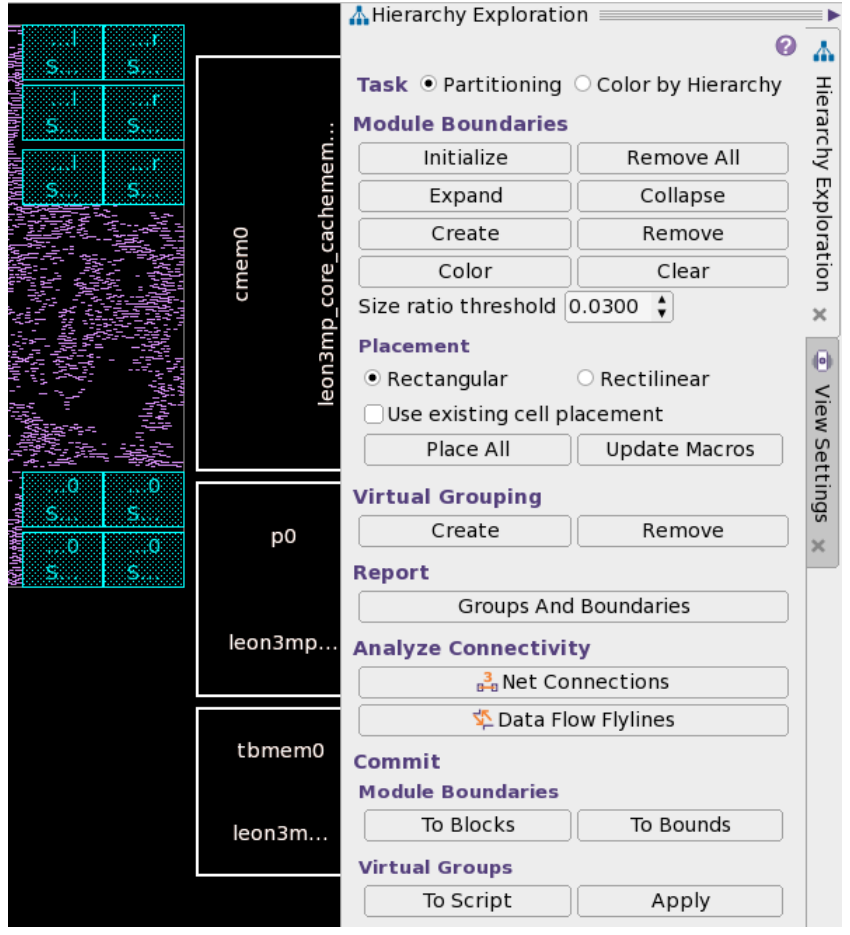
\includegraphics[width=0.92\textwidth]{gui-fig-068.png}
\caption{初始化后的模块边界}
\label{fig:gui-68}
\end{figure}

可以用 \cmd{explore\_logic\_hierarchy -create\_module\_boundary} 命令执行同一操作。

也可以用 GUI 中的 Hierarchy Browser 为所选模块创建模块边界。用 Hierarchy Browser 创建模块边界：
\begin{enumerate}
  \item 选择 \textbf{View > Hierarchy Browser}
  \item 选择一个逻辑层次块
  \item 从上下文菜单选择 Create Module Boundary，或单击 Hierarchy Exploration 面板 Module Boundaries 区中的 Create 按钮
\end{enumerate}

\subsection{展开、折叠与删除模块边界}
\subsubsection*{Expanding, Collapsing, and Removing Module Boundaries}

要把模块边界展开为子模块，选择该模块边界并单击 Expand。要把模块边界折叠进其父模块，选择该模块边界并单击 Collapse。要删除一个或多个模块边界，选择这些模块边界并单击 Remove。要删除全部模块边界，单击 Remove All。

也可以用上下文菜单执行这些操作。
\begin{enumerate}
  \item 选择一个或多个模块边界
  \item 在所选模块边界之一上右键单击，并从上下文菜单选择操作（Expand、Collapse 或 Remove Module Boundary）
\end{enumerate}

\subsection{为模块边界着色}
\subsubsection*{Coloring Module Boundaries}

要为每个模块边界应用互不相同的颜色，单击 Color。再次单击 Color，应用另一种配色方案。要去掉模块边界上的任何着色，单击 Clear。

\subsection{放置模块边界}
\subsubsection*{Placing Module Boundaries}

要把模块边界放入核区域（core area）：
\begin{enumerate}
  \item 选择布局类型：矩形（rectangular）或直角多边形（rectilinear）。两种布局类型的示例见图~\ref{fig:gui-69}
  \item 选择 Use existing cell placement，按已有布局放置模块边界
  \item 单击 Place All，把模块边界放入核区域
\end{enumerate}

\begin{figure}[htbp]
\centering
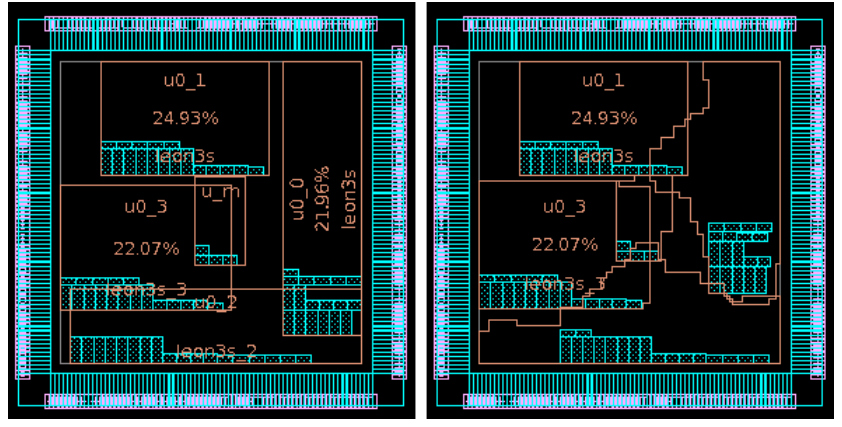
\includegraphics[width=0.92\textwidth]{gui-fig-069.png}
\caption{矩形与直角多边形模块边界布局}
\label{fig:gui-69}
\end{figure}

要把属于某个模块约束的硬宏移入模块边界内部，单击 Update Macros。

\subsection{层次探索与模块颜色}
\subsubsection*{Hierarchy Exploration and Module Color}

Hierarchy Exploration 面板提供工具，为模块边界以及设计边界内与之对应的标准单元和宏添加颜色。工具还会在设计内不同层次周围画出边界。在面板顶部 Task 区中选择 “Color by Hierarchy”，即可使用这些功能。

\begin{figure}[htbp]
\centering
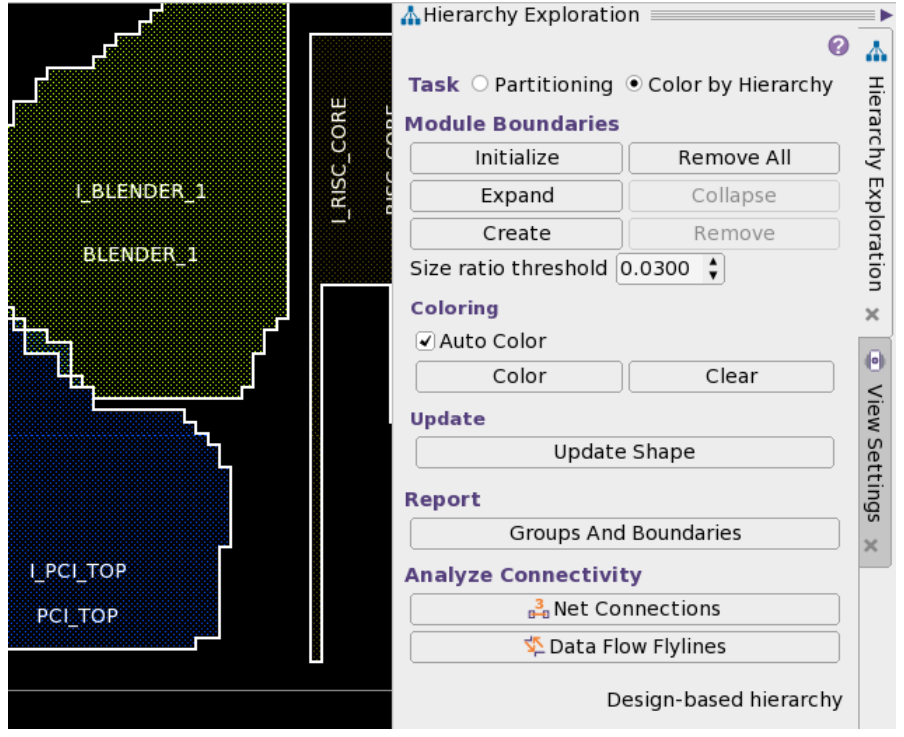
\includegraphics[width=0.92\textwidth]{gui-fig-070.png}
\caption{层次探索中的按层次着色}
\label{fig:gui-70}
\end{figure}

\subsection{在版图中查看层次}
\subsubsection*{Viewing Hierarchies in the Layout}

要在版图中高亮不同层次：
\begin{enumerate}
  \item 从菜单选择 \textbf{View > Assistants > Hierarchy Exploration}。
  \item 在面板的 Task 区中选择 “Color by Hierarchy”。
  \item 在面板的 Module Boundaries 区单击 Initialize，创建模块边界。
\end{enumerate}

工具高亮并选择全部顶层层次。
\begin{enumerate}
  \setcounter{enumi}{3}
  \item （可选）单击 Color 更改模块颜色，单击 Clear 去掉全部模块颜色。
  \item （可选）打开 Hierarchy Browser 并选择一个或多个层次，更改被高亮的层次。
\end{enumerate}

\subsection{假设划分}
\subsubsection*{What-if Partitioning}

假设划分（what-if partitioning）帮助查看不同模块边界之间的关系，并通过创建虚拟组（virtual group）来组织模块边界的层次。在假设划分期间，可以：
\begin{itemize}
  \item 用 Net Connections 或 Data Flow Flylines 工具查看不同模块边界之间的连接关系
  \item 创建包含相互连接的模块边界的虚拟组
  \item 通过放置、合并或删除虚拟组，考察不同的划分策略
  \item 写出模块边界分组，供重新综合（resynthesis）使用
\end{itemize}

要显示模块边界之间的连接关系：
\begin{enumerate}
  \item 单击 Hierarchy Exploration 面板中的 Net Connections 按钮。
  \item 在 Net Connections 面板的 Connectivity Display 区中选择 Selected to Selected。
  \item 单击一个模块边界，再单击一个或多个其他边界，查看它们之间的连接关系。
\end{enumerate}

要创建虚拟组：
\begin{enumerate}
  \item 只选择要合并进新模块组的模块边界或模块组。
  \item 单击 Hierarchy Exploration 面板 Virtual Grouping 区中的 Create 按钮。
  \item （可选）选择某个虚拟组并单击 Remove 按钮，取消该虚拟组的分组。
\end{enumerate}

图~\ref{fig:gui-71} 左侧，两个模块边界被选中，并显示了所选模块的线网连接。这两个模块共享公共线网连接，适合分在一组。右侧是单击 Create 按钮后已分组的模块。可以把指针移到模块组上，在信息提示中显示该组的信息。

\begin{figure}[htbp]
\centering
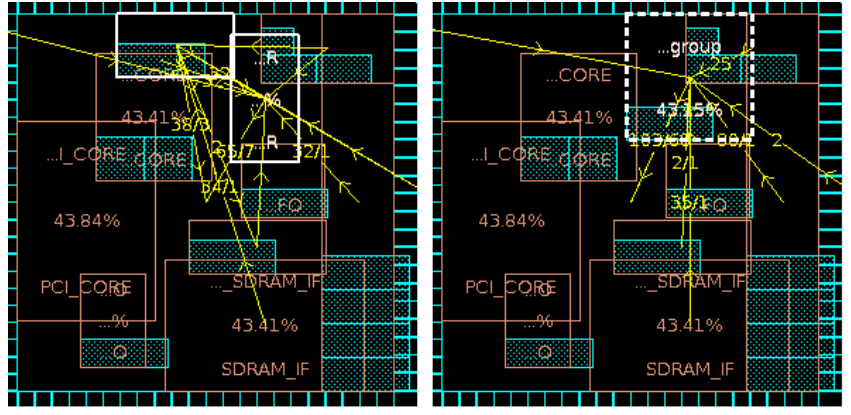
\includegraphics[width=0.92\textwidth]{gui-fig-071.png}
\caption{为两个模块创建虚拟组}
\label{fig:gui-71}
\end{figure}

若选择中包含已有虚拟组以及其他模块边界，这些模块边界会被加入该已有虚拟组。

创建模块边界的虚拟组之后，要报告版图中当前的模块边界与组，单击 Report 区中的 Groups and Boundaries 按钮。工具打开 Groups and boundaries 面板，并显示版图中的虚拟组与模块边界列表。工具还会把信息写入 \cmd{module\_boundary.results} 文件，内容如下：
\begin{lstlisting}
icc2_shell> sh cat module_boundary.results
virtual group:   RISC_CORE_group
                 I_ORCA_TOP/I_RISC_CORE
                 I_ORCA_TOP/I_PCI_TOP
                 I_ORCA_TOP/I_BLENDER_4
module boundary: I_CLOCK_GEN
module boundary: I_ORCA_TOP/I_SDRAM_TOP
...
***** End Of Report *****
\end{lstlisting}

要用虚拟组生成一份包含 Tcl 命令的脚本，以便创建新的层次级别，单击 Virtual Groups 区中的 To Script 按钮。工具打开 Script Editor，并写入 \cmd{group\_cells} 与 \cmd{explore\_logic\_hierarchy} 命令，用来从虚拟组重新创建新的层次级别。示例脚本如下：
\begin{lstlisting}
### Virtual Grouping Commands For Group: RISC_CORE_group
group_cells { I_ORCA_TOP/I_RISC_CORE I_ORCA_TOP/I_PCI_TOP \
              I_ORCA_TOP/I_BLENDER_4 } -cell_name RISC_CORE_group
if { [get_bounds -quiet RISC_CORE_group] ne {} } {
    explore_logic_hierarchy -virtual_ungroup RISC_CORE_group
    explore_logic_hierarchy -create_module_boundary \
       -cell [get_cells -quiet -hierarchical RISC_CORE_group]
}
### End Virtual Grouping Commands For Group: RISC_CORE_group
\end{lstlisting}

要把所选模块边界提交为块，单击 Hierarchy Exploration 面板 Commit 区中的 To Blocks。

要把所选模块边界提交为约束，单击 Hierarchy Exploration 面板 Commit 区中的 To Bounds。

\section{拓扑管脚约束}
\subsection*{Topological Pin Constraints}

拓扑管脚约束（Topological Pin Constraints）工具可以在 GUI 中创建管脚约束（pin constraint）：指定一条线网，并画出馈通（feedthrough）必须在其中布线的矩形区域。要启动 Topological Pin Constraints 工具，从菜单选择 \textbf{Create > Topological Pin Constraint}，或单击相应工具栏按钮。要查看或编辑管脚约束的信息，单击图~\ref{fig:gui-72} 中圈出的按钮，打开 Topological Pin Constraints 对话框。

\begin{figure}[htbp]
\centering
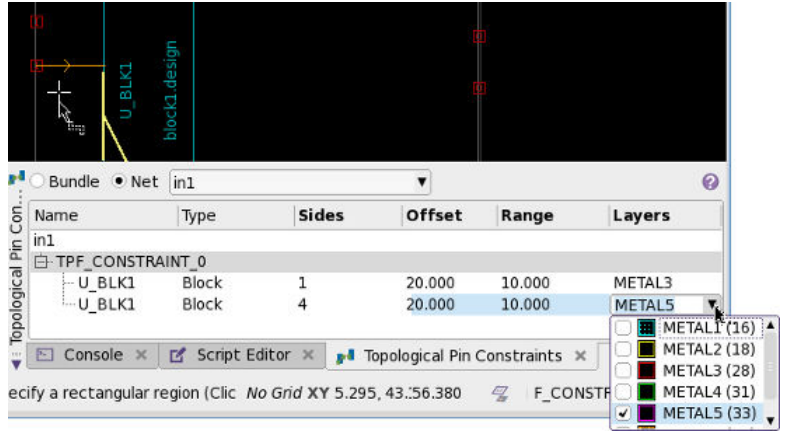
\includegraphics[width=0.92\textwidth]{gui-fig-072.png}
\caption{拓扑管脚约束}
\label{fig:gui-72}
\end{figure}

要为含有多级层次的设计创建拓扑管脚约束，单击 View Settings 面板中的 multiple levels active 框，如下图所示。

\begin{figure}[htbp]
\centering
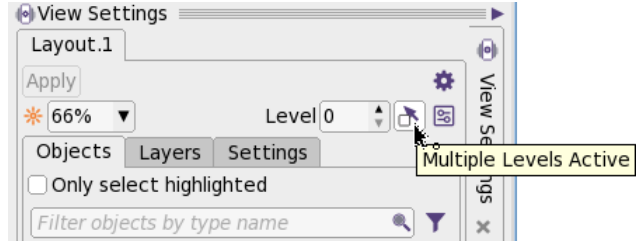
\includegraphics[width=0.92\textwidth]{gui-fig-073.png}
\caption{多级层次处于活动状态}
\label{fig:gui-73}
\end{figure}

\section{使用管脚约束}
\subsection*{Working With Pin Constraints}

使用 Design Assistant 创建、显示和修改单个、成束以及块级管脚约束。

\begin{longtable}{@{}>{\raggedright\arraybackslash}p{0.32\textwidth}>{\raggedright\arraybackslash}p{0.64\textwidth}@{}}
\caption{GUI 支持的管脚约束操作}\label{tab:gui-dp-pin}\\
\toprule
要执行的操作 & 使用此方法 \\
\midrule
\endfirsthead
\caption*{表~\thetable{}（续）：GUI 支持的管脚约束操作}\\
\toprule
要执行的操作 & 使用此方法 \\
\midrule
\endhead
\bottomrule
\endlastfoot
创建管脚约束 &
1. \textbf{Design Assistant > Nets}（或）\textbf{Design Assistant > Pins}\newline
2. 选择线网或束（bundle）（或）选择端口或管脚\newline
3. \textbf{Create > Pin Constraint} \\
\addlinespace
创建块约束 &
在 Design Assistant 中选择 \textbf{Create > Block Pin Constraint} \\
\addlinespace
查看当前设计中的管脚约束与块管脚约束 &
在 Design Assistant 中选择：\newline
\textbullet\ \textbf{View > Pin Constraints of selected}（或）\newline
\textbullet\ \textbf{View > Block Pin Constraints of selected}（或）\newline
\textbullet\ \textbf{View > Pin Constraints}（或）\newline
\textbullet\ \textbf{View > Block Pin Constraints} \\
\addlinespace
显示所选对象上当前已定义的管脚约束 &
在 Design Assistant 中：\newline
1. 选择线网或管脚\newline
2. 右键单击并选择 Get Pin Constraints（或）\textbf{View > Pin Constraints of selected}\newline
管脚约束显示在 PinConstraints 选项卡上。 \\
\addlinespace
显示所选对象上当前已定义的块管脚约束 &
在 Design Assistant 中：\newline
1. 选择块单元（\cmd{is\_soft\_macro == true}）\newline
2. 右键单击并选择 Get Block Pin Constraints（或）\textbf{View > Block Pin Constraints of selected}\newline
管脚约束显示在 BlockPinConstraints 选项卡上。 \\
\addlinespace
删除管脚约束与块管脚约束 &
在 Design Assistant 中选择 \textbf{Edit > Delete Pin Constraints} \\
\addlinespace
选择与管脚约束相关的对象 &
选择管脚约束，再选择 \textbf{Select > Related Objects}，以选择相关的束、线网、管脚或端口 \\
\end{longtable}

% 第 4 章续：拓扑互连规划
\section{执行拓扑互连规划}
\subsection*{Performing Topology Interconnect Planning}

可以用拓扑互连规划（topology interconnect planning）方法，为大量总线信号定义并创建布线拓扑。

\begin{seeAlsoBox}
更多说明见 \emph{IC Compiler II Design Planning User Guide} 中的 Topology Interconnect Planning。
\end{seeAlsoBox}

在拓扑互连规划流程中，统一拓扑约束（unified topology constraint，UTC）为版图中总线信号的布线拓扑提供一种共同的约束语言和方法。UTC 的基本构成是拓扑规划（topology plan）、拓扑节点（topology node）、拓扑边（topology edge）和拓扑中继器（topology repeater）。

下列各节说明可以在 GUI 中对这些构件执行的部分操作。
\begin{itemize}
  \item 使用 Topology Toolbox
  \item 使用 Create Topology Layout 工具
  \item 用定制符号表示拓扑节点
  \item 使用 Move Topology Object 工具
  \item 把拓扑节点附着到有效的重叠对象
  \item 把拓扑节点连成菊花链
  \item 设置拓扑边的形状层
  \item 使用拓扑组与拓扑规划
  \item 使用束对象
  \item 在 GUI 中查看拓扑时序估算结果
\end{itemize}

\subsection{使用 Topology Toolbox}
\subsubsection*{Using the Topology Toolbox}

可以从 Topology Toolbox（\textbf{View > Toolbars > Topology Toolbox} 或 \textbf{View > Assistants > Topology Toolbox}）访问全部与拓扑互连规划相关的命令和实用功能。

\begin{longtable}{@{}>{\raggedright\arraybackslash}p{0.16\textwidth}>{\raggedright\arraybackslash}p{0.24\textwidth}>{\raggedright\arraybackslash}p{0.54\textwidth}@{}}
\caption{Topology Toolbox}\label{tab:gui-dp-toolbox}\\
\toprule
区段 & 工具界面 & 说明 \\
\midrule
\endfirsthead
\caption*{表~\thetable{}（续）：Topology Toolbox}\\
\toprule
区段 & 工具界面 & 说明 \\
\midrule
\endhead
\bottomrule
\endlastfoot
工具栏（Toolbar） & 下列按钮 &
\textbullet\ Design Assistant：执行设计规划任务\newline
\textbullet\ Create Topology Layout：创建节点、边、中继器等拓扑对象\newline
\textbullet\ Lock：把所选对象锁定在当前位置以便编辑\newline
\textbullet\ Unlock：解除所选对象的锁定\newline
\textbullet\ Set topology objects visible：把拓扑对象设为可见\newline
\textbullet\ Set topology objects invisible：把拓扑对象设为不可见\newline
\textbullet\ Set net estimation rule：设置线网估算规则\newline
\textbullet\ Associate selected annotation shapes with topology plan：把所选或当前拓扑规划与所选标注形状（annotation shape）关联。若选择了不止一个拓扑规划，该操作被禁用。把标注形状与拓扑规划关联之后，其可见性由所关联拓扑规划的可见性决定，并同时受 View Settings 面板中标注形状可见性设置的影响。 \\
\addlinespace
规划（Plan） & 下列按钮 &
\textbullet\ Create：创建拓扑规划\newline
\textbullet\ Characterize：特征化（characterize）拓扑规划\newline
\textbullet\ Create Default：创建默认拓扑规划\newline
\textbullet\ Refine：细化（refine）拓扑规划\newline
\textbullet\ Create Group：创建拓扑组\newline
\textbullet\ Uniquify：唯一化（uniquify）拓扑规划\newline
\textbullet\ Optimize：优化拓扑规划\newline
\textbullet\ Write：写出拓扑规划 \\
\addlinespace
选择（Select） & 用于下列操作的按钮 &
\textbullet\ 选择相关拓扑规划\newline
\textbullet\ 选择相关拓扑边\newline
\textbullet\ 选择相关拓扑节点\newline
\textbullet\ 选择相关拓扑中继器\newline
\textbullet\ 选择相连的拓扑 \\
\addlinespace
编辑（Edit） & 用于下列操作的按钮 &
\textbullet\ 移动或附着拓扑对象\newline
\textbullet\ 合并拓扑节点\newline
\textbullet\ 删除所选拓扑节点\newline
\textbullet\ 把有效的重叠对象与所选拓扑节点关联\newline
\textbullet\ 删除与拓扑规划关联的布线 \\
\addlinespace
边（Edge） & 用于下列操作的按钮 &
\textbullet\ 用不同选项自动循环形状。循环顺序：Auto $\rightarrow$ L-Shape (x) $\rightarrow$ L-Shape (y) $\rightarrow$ S-Shape (x) $\rightarrow$ S-Shape (y)\newline
\textbullet\ 自动设置边的形状\newline
\textbullet\ Set edge L-Shape (X-First)，即先水平\newline
\textbullet\ Set edge L-Shape (Y-First)，即先垂直\newline
\textbullet\ Set edge S-Shape (X-First)\newline
\textbullet\ Set edge S-Shape (Y-First)\newline
\textbullet\ 反转边的方向\newline
\textbullet\ 按线网估算规则设置边的层\newline
\textbullet\ 估算拓扑边\newline
\textbullet\ 重置拓扑边估算，即把边形状的宽度重置为零 \\
\addlinespace
连接（Connection） & 用于下列操作的按钮 &
\textbullet\ 创建鱼骨连接（fishbone connection）\newline
\textbullet\ 创建链式连接（chain connection）\newline
\textbullet\ 创建星形连接（star connection）\newline
\textbullet\ 向左连接节点\newline
\textbullet\ 向右连接节点\newline
\textbullet\ 向上连接节点\newline
\textbullet\ 向下连接节点 \\
\addlinespace
分析（Analyze） & 用于下列操作的按钮 &
\textbullet\ 检查拓扑规划\newline
\textbullet\ 估算拓扑规划 \\
\addlinespace
实现（Implement） & 用于下列操作的按钮 &
\textbullet\ 创建拓扑干线（trunk）\newline
\textbullet\ 实现拓扑中继器\newline
\textbullet\ 删除与拓扑规划关联的布线\newline
\textbullet\ 删除所选拓扑规划上已放置和已创建的中继器 \\
\end{longtable}

\subsubsection{定制 Topology Toolbox}
\subsubsection*{Customizing the Topology Toolbox}

要把常用操作加入 Topology Toolbox，可以定制该工具箱，并把操作加到一个新的 User 区。

下面的示例向 Topology Toolbox 加入两个按钮 Nudge Left 与 Nudge Right，使视图略向左和向右平移。
\begin{lstlisting}
gui_create_menu -menu "My_Menu->&Nudge_Right" \
   -tcl_cmd {gui_scroll \
   -window [gui_get_current_window -view] -hrel .05}
gui_create_menu -menu "My_Menu->&Nudge_Left" \
   -tcl_cmd {gui_scroll \
   -window [gui_get_current_window -view] -hrel -.05}
gui_set_pref_value -category topologyToolbox \
   -key userButtonsList -value "My_Menu->Nudge_Right My_Menu->Nudge_Left"
\end{lstlisting}

\subsection{使用 Create Topology Layout 工具}
\subsubsection*{Using the Create Topology Layout Tool}

要创建节点、边、中继器等拓扑对象，使用 Create Topology Layout 工具。也可以为形状层创建带混合值（百分比与距离）的拓扑边。

用该工具定义凸点区域（bump region）之间的连接，以建立芯片到芯片的连接。也可以像对待任何其他有效对象一样，用 \cmd{create\_topology\_node} 命令把拓扑节点与凸点区域关联；可在 Create Topology Layout 工具、Move Topology Object 工具中执行，或通过 Properties Editor 执行。

可以按下列方式使用拓扑版图工具：
\begin{enumerate}
  \item 在 \textbf{Design Assistant > Topologies} 选项卡中选择一个拓扑规划。
  \item 用下列方法之一打开 Create Topology Layout 工具栏：
  \begin{itemize}
    \item 在 \textbf{Design Assistant > Topologies} 选项卡中选择 \textbf{Create > Topology Layout}。
    \item 在 \textbf{Design Assistant > Topologies} 选项卡中，右键单击拓扑规划，再单击 Topology Layout。
    \item 在块窗口中选择 \textbf{Create > Topology Layout}。
  \end{itemize}
\end{enumerate}

\begin{figure}[htbp]
\centering
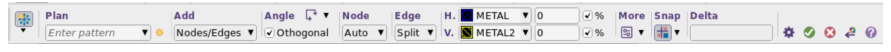
\includegraphics[width=0.92\textwidth]{gui-fig-074.png}
\caption{创建拓扑版图工具栏}
\label{fig:gui-74}
\end{figure}

\begin{enumerate}
  \setcounter{enumi}{2}
  \item 在版图视图中，单击要连接的拓扑节点对象，或从新的拓扑节点开始。
  \item 把光标移到下一个目标，它可以是已有的或新的拓扑节点。移动指针时，工具只勾勒出可以与新节点关联的对象。
  \item 单击鼠标按钮以放置节点。
  \item 单击末端对象（拓扑节点）以完成布线，或双击以用新节点结束。
\end{enumerate}

要把选项重置为默认值，使用 Create Topology Layout 工具栏上的相应图标（见图~\ref{fig:gui-74}）。

要撤销所做的更改，选择 \textbf{Edit > Undo}。

\begin{longtable}{@{}>{\raggedright\arraybackslash}p{0.32\textwidth}>{\raggedright\arraybackslash}p{0.64\textwidth}@{}}
\caption{Create Topology Layout 工具选项}\label{tab:gui-dp-layout}\\
\toprule
选项 & 说明 \\
\midrule
\endfirsthead
\caption*{表~\thetable{}（续）：Create Topology Layout 工具选项}\\
\toprule
选项 & 说明 \\
\midrule
\endhead
\bottomrule
\endlastfoot
Plan & 指定新节点、边和中继器所加入的拓扑规划名称。创建拓扑规划。 \\
\addlinespace
Add & 指定要添加的对象类型。 \\
\addlinespace
Angle & 在正交输入模式（orthogonal input mode）下设置起始输入方向。 \\
\addlinespace
Orthogonal & 切换正交输入方向。 \\
\addlinespace
Node & 指定拓扑节点的节点约束类型。 \\
\addlinespace
Edge & 设为 Split 时，在拓扑边中点插入新节点，把最后一条边拆成两条；否则创建抽头节点（tap node）。 \\
\addlinespace
Horizontal Layer/Width/Length Percentage & 指定水平边的形状层与宽度。选中水平长度百分比选项时，工具按百分比设置水平边形状长度；否则边长设为绝对长度。 \\
\addlinespace
Vertical Layer/Width/Length Percentage & 指定垂直边的形状层与宽度。选中垂直长度百分比选项时，工具按百分比设置垂直边形状长度；否则边长设为绝对长度。 \\
\addlinespace
Snap & 打开或关闭把拓扑节点吸附（snap）到可见或可选对象。 \\
\addlinespace
Delta & 为版图编辑输入点时，指定相对活动推断点（inference point）的偏移信息。 \\
\addlinespace
More > Node > Attach & 设为 true 时，预选并标注该节点可以附着的有效对象。 \\
\addlinespace
More > Node > Prefer pins & 设为 true 时，把拓扑节点与管脚关联，而不是与块关联。 \\
\addlinespace
More > Node > Routing target & 指定约束类型为 edge、side 和 bounding box 的节点能否作为布线目标。 \\
\addlinespace
More > Actions > Auto apply & 设为 true 时，新节点（边的末端节点）关联到任何有效对象（块、管脚、端口等）后即结束输入。 \\
\addlinespace
More > Show > Port Guidance & 显示管脚连接与位置的引导。 \\
\addlinespace
More > Show > Flylines & 显示指定线网的管脚飞线（flyline），或到最近开口（open）的飞线。 \\
\addlinespace
More > Show > Routes & 高亮指定的线网或束。 \\
\end{longtable}

\subsection{用定制符号表示拓扑节点}
\subsubsection*{Using Custom Symbols to Represent Topology Nodes}

默认情况下，工具用下列约定表示拓扑节点。

\begin{table}[htbp]
\centering
\caption{拓扑节点的默认符号}
\label{tab:gui-dp-nodesym}
\begin{tabularx}{\textwidth}{@{}l X@{}}
\toprule
拓扑节点 & 符号 \\
\midrule
起始节点（start node） & 圆（circle） \\
中间节点（intermediate node） & 菱形（diamond） \\
结束节点（end node） & 正方形（square） \\
\bottomrule
\end{tabularx}
\end{table}

需要时，可以用定制符号表示这些节点。要使用定制符号：
\begin{enumerate}
  \item 在 Layout View 中选择该节点。
  \item 打开 Properties Editor。
  \item 切换到 Application 属性组。
  \item 从 symbol 下拉列表中选择一种符号。
  \item 单击 Apply Changes。
\end{enumerate}

\subsection{使用 Move Topology Object 工具}
\subsubsection*{Using the Move Topology Object Tool}
\label{sec:gui-dp-move}

要移动拓扑节点，以及把拓扑节点与允许的对象关联或解除关联，使用 Move Topology Object 工具。若要同时自动关联许多拓扑节点，见第~\ref{sec:gui-dp-attach}~节。

\begin{figure}[htbp]
\centering

\includegraphics[width=0.92\textwidth]{gui-fig-075.png}
\caption{移动拓扑对象工具栏}
\label{fig:gui-75}
\end{figure}

流程如下：
\begin{enumerate}
  \item 选择 \textbf{Edit > Topology > Move}。
  \item 单击要修改的拓扑节点。
  \item 把节点移到新位置。
\end{enumerate}

要把选项重置为默认值，使用 Move Topology Object 工具栏上的相应图标（见图~\ref{fig:gui-75}）。

要撤销所做的更改，选择 \textbf{Edit > Undo}。

Move Topology Object 工具栏上的 Node、Edge、More、Snap 和 Delta 选项，与 Create Topology Layout 工具栏上的对应选项行为相同。详见第~\ref{tab:gui-dp-layout}~表。

要让拓扑边的形状层使用层颜色，或为起始、中间和结束拓扑节点使用不同颜色，按图~\ref{fig:gui-76} 所示使用相应选项。

\begin{figure}[htbp]
\centering
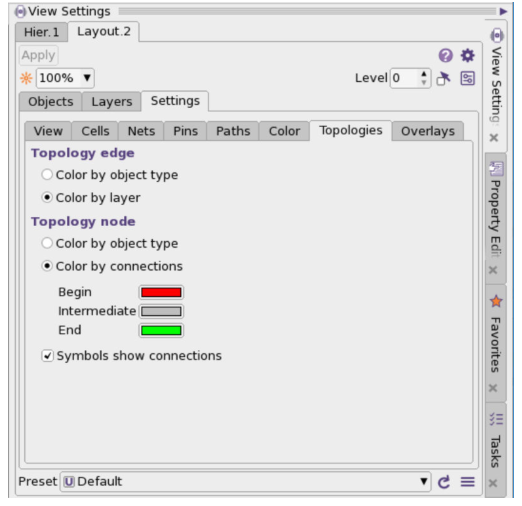
\includegraphics[width=0.92\textwidth]{gui-fig-076.png}
\caption{为拓扑边与拓扑节点使用着色}
\label{fig:gui-76}
\end{figure}

\subsection{把拓扑节点附着到有效的重叠对象}
\subsubsection*{Attaching Topology Nodes With Valid Overlapped Objects}
\label{sec:gui-dp-attach}

在把拓扑规划或边复制或移动到目标位置时，要自动把拓扑节点附着到与这些节点重叠的有效对象，使用 \cmd{attach\_topology\_nodes} 命令。若要逐个附着拓扑节点，使用 Move Topology Object 工具（详见第~\ref{sec:gui-dp-move}~节）。

有效的重叠对象包括：
\begin{itemize}
  \item 标注形状（annotation shape）
  \item 约束（bound）
  \item 约束形状（bound shape）
  \item 凸点区域（bump region）
  \item 单元（cell）
  \item 管脚（pin）
  \item 端口（port）
  \item 形状（shape）
  \item 布局阻塞（placement blockage）
  \item 布线阻塞（routing blockage）
  \item 拓扑边（topology edge）
  \item 端子（terminal）
  \item 电压区域（voltage area）
  \item 电压区域形状（voltage area shape）
\end{itemize}

存在许多重叠对象时，管脚和端口的优先级高于单元，单元的优先级高于其他类型的对象。

在下面的示例中，工具尝试把拓扑规划 tp1 中的全部拓扑节点附着到有效对象。
\begin{lstlisting}
icc2_shell> attach_topology_nodes [get_topology_nodes \
   -of_objects [get_topology_plans tp1]]
\end{lstlisting}

\begin{seeAlsoBox}
更多说明见 \cmd{attach\_topology\_nodes} 命令的 man 页。
\end{seeAlsoBox}

\subsection{把拓扑节点连成菊花链}
\subsubsection*{Daisy Chaining Topology Nodes}

要在当前块中按给定方向快速连接所选或指定的拓扑节点，即把它们连成菊花链（daisy chain）：
\begin{enumerate}
  \item 在版图视图中选择要连接的拓扑节点。
  \item 在指定方向上于所选节点之间创建拓扑边：选择 \textbf{Edit > Topology > Connect Nodes Down}（Up、Left、Right）。
\end{enumerate}

也可以使用相应的上下文相关菜单命令，或 \cmd{connect\_topology\_nodes} 命令。

\begin{noteBox}
若某些节点已经相连，它们会被排除在该操作之外。
\end{noteBox}

\begin{table}[htbp]
\centering
\caption{连接拓扑节点}
\label{tab:gui-dp-connect}
\begin{tabularx}{\textwidth}{@{}XXXX@{}}
\toprule
向下连接拓扑节点 & 向上连接拓扑节点 & 向左连接拓扑节点 & 向右连接拓扑节点 \\
\midrule
版图示意 & 版图示意 & 版图示意 & 版图示意 \\
\bottomrule
\end{tabularx}
\end{table}

\subsection{设置拓扑边的形状层}
\subsubsection*{Setting Topology Edge Shape Layers}

本工具可以为所选或指定的拓扑边设置形状层，或反转其方向。
\begin{enumerate}
  \item 在版图视图中，选择需要设置形状层的拓扑边。
  \item 选择 \textbf{Edit > Topology}，再执行下列操作之一：
\end{enumerate}

\begin{table}[htbp]
\centering
\caption{为拓扑边设置形状层}
\label{tab:gui-dp-shapelayer}
\begin{tabularx}{\textwidth}{@{}X l@{}}
\toprule
要执行的操作 & 使用此功能 \\
\midrule
第一段沿 x 方向的 L 形 & Set Edge L-Shape (X First) \\
第一段沿 y 方向的 L 形 & Set Edge L-Shape (Y First) \\
第一段沿 x 方向的 S 形 & Set Edge S-Shape (X First) \\
第一段沿 y 方向的 S 形 & Set Edge S-Shape (Y First) \\
按起始与结束拓扑节点的接入方向自动选择形状模板 & Set Topology Edge Auto \\
交换起始节点与结束节点，从而反转边的方向 & Reverse Topology Edge Direction \\
按线网估算规则的层定义更新边的形状层 & Set Edge NER Layers \\
\bottomrule
\end{tabularx}
\end{table}

\subsection{使用拓扑组与拓扑规划}
\subsubsection*{Working With Topology Groups and Topology Plans}

\begin{itemize}
  \item 设置当前拓扑组
  \item 删除拓扑组
  \item 查看并编辑拓扑组的聚合属性
  \item 唯一化拓扑规划
  \item 自动选择拓扑规划
  \item 合并堆叠的拓扑节点
\end{itemize}

拓扑组可以把拓扑规划分成多个更小的组。随后可以独立处理这些较小的部分，从而把大型设计分成可管理的部分。它也可以把相似的拓扑规划分在一组，以便对一组拓扑规划执行修改、删除等操作。

流程如下：
\begin{enumerate}
  \item 创建线网估算规则（net estimation rule）。

  线网估算规则定义布线层、非默认布线规则（nondefault routing rule）、中继器单元名、中继器单元间距、时钟，以及其他与布线和时序相关的约束。创建拓扑规划之后，把一条线网估算规则与该拓扑规划关联。需要时，可以从 Properties Editor 面板、Design Assistant，或从自动生成的命令表单（例如 \cmd{create\_topology\_plan} 命令对话框）为一条拓扑规划或一条拓扑边关联多条线网估算规则。
  \begin{enumerate}[label=\alph*.]
    \item 选择 \textbf{View > Assistants > Design Assistant}，打开 Design Assistant。
    \item 选择 \textbf{Create > Net Estimation Rule}。
    \item 按需要在 \cmd{set\_net\_estimation\_rule} 对话框中输入信息，再单击 OK。
  \end{enumerate}

  也可以用 Design Assistant 的 TopologyPlans 与 TopologyGroups 选项卡上的上下文相关菜单创建线网估算规则（在拓扑规划或拓扑组上右键单击，再从菜单选择 Create Net Estimation Rule）。

  \begin{seeAlsoBox}
  关于为拓扑规划创建线网估算规则的更多说明，见 \emph{IC Compiler II Design Planning User Guide} 中的 Creating Net Estimation Rules for Topology Plans。
  \end{seeAlsoBox}

  \item 为线网创建拓扑规划。
  \begin{enumerate}[label=\alph*.]
    \item 单击 Nets 选项卡，用 \cmd{get\_nets} 命令填充列表。
    \item 从列表中选择线网，右键单击所选内容，再选择 Create Topology Plan。
    \item 按需要在 \cmd{create\_topology\_plan} 对话框中输入信息，再单击 OK。
    \item 选择 \textbf{View > New topology Plans}，打开 TopologyPlans 选项卡。
    \item 在 TopologyPlans 选项卡上，用 \cmd{get\_topology\_plans} 命令查看新创建的拓扑规划。
    \item 按需要创建足够多的拓扑规划。
  \end{enumerate}

  创建时，全部拓扑规划都被分配到默认拓扑组 \cmd{DEFAULT\_TOPOLOGY\_GROUP}。group 列显示该拓扑规划所关联的拓扑组。也可以在拓扑规划上右键单击，并从上下文相关菜单选择 Get Topology Group，查看它所属的拓扑组。

  用下列步骤把拓扑规划重新分配到指定的拓扑组。

  \item 为特定拓扑规划创建拓扑组。
  \begin{enumerate}[label=\alph*.]
    \item 在 TopologyPlans 选项卡上，从列表中选择拓扑规划，右键单击所选内容，再选择 Create Topology Group。

    一个拓扑规划只属于一个拓扑组。不能在多个拓扑组之间共享拓扑规划。
    \item 按需要在 \cmd{create\_topology\_group} 对话框中输入信息，再单击 OK。
  \end{enumerate}

  若为拓扑组指定了名称，且当前块中已存在该名称，工具会报错。不过，设计的不同块中可以有同名的拓扑组。若不为拓扑组指定名称，工具自动分配格式为 \cmd{TOPOLOGY\_GROUP<\#n>} 的名称，其中 n 是从 1 开始的整数。

  \begin{noteBox}
  若一个拓扑组包含多个规划，且这些规划在某个属性上的值不同，工具把该属性的值显示为 \cmd{<mixed>}。例如，拓扑组 TG1 有两个拓扑规划 TP1 与 TP2，颜色分别为红色和蓝色，则在 TopologiesGroup 选项卡中，颜色列显示 \cmd{<mixed>}。

  可以把显示为 \cmd{<mixed>} 的值更新为符合要求的值。但不能把属性设为 \cmd{<mixed>}。若提供的值对该属性无效，工具会报错。
  \end{noteBox}

  \begin{seeAlsoBox}
  关于创建拓扑组的更多说明，见 \emph{IC Compiler II Design Planning User Guide} 中的 Creating Topology Groups。
  \end{seeAlsoBox}
\end{enumerate}

把拓扑规划与拓扑组关联之后，可以在 TopologyPlans 选项卡的 group 列中查看这一关联。

要处理一组特定的拓扑规划：
\begin{enumerate}
  \item 在 TopologiesGroups 选项卡上，选择相关的拓扑组。

  若创建拓扑组时添加了注释，可以用 comment 列中的这一信息挑选相关拓扑组。
  \item 右键单击所选拓扑组，并选择 Get Topology Plans。
\end{enumerate}

属于该拓扑组的拓扑规划显示在 TopologiesPlans 选项卡上。可以从 GUI 中提供的选项对这些拓扑规划执行必要操作。

要查看特定拓扑组中的拓扑规划：
\begin{enumerate}
  \item 在 TopologiesGroups 选项卡上，选择拓扑组。
  \item 选择 \textbf{View > Toolbars > Constraints Editor}。
\end{enumerate}

这一步打开 Constraints Editor 视图，列出属于所选拓扑组的全部拓扑规划，以及它们的拓扑节点和边。

\subsubsection{设置当前拓扑组}
\subsubsection*{Setting the Current Topology Group}

创建拓扑组时，它成为当前拓扑组。

要把某个拓扑组设为当前拓扑组：
\begin{enumerate}
  \item 在 TopologiesGroups 选项卡上，选择相关的拓扑组。
  \item 选择 \textbf{Edit > Topology > Set Current Group}，或在 Design Assistant 的上下文菜单中选择 Set Current Topology Group。
\end{enumerate}

\begin{seeAlsoBox}
关于创建拓扑组的更多说明，见 \emph{IC Compiler II Design Planning User Guide} 中的 Setting the Current Topology Group。
\end{seeAlsoBox}

\subsubsection{删除拓扑组}
\subsubsection*{Removing Topology Groups}

不再需要一个或多个拓扑组时，可以选择这些拓扑组，再选择 \textbf{Edit > Topology > Remove Group} 菜单，从 GUI 中删除它们。删除含有拓扑规划的拓扑组时，工具自动把这些拓扑规划移到默认拓扑组。若默认拓扑组中还有任何拓扑规划，则不能删除默认拓扑组；不过可以对 \cmd{remove\_topology\_groups} 命令使用 \opt{-remove\_plans} 选项，同时删除拓扑规划和默认拓扑组。

\begin{seeAlsoBox}
关于创建拓扑组的更多说明，见 \emph{IC Compiler II Design Planning User Guide} 中的 Removing Topology Groups。
\end{seeAlsoBox}

\subsubsection{查看并编辑拓扑组的聚合属性}
\subsubsection*{Viewing and Editing Aggregate Attributes of Topology Groups}

IC Compiler II 工具支持编辑拓扑组的聚合属性。

当拓扑组中不同拓扑规划在某个属性上的值不同时，工具聚合该属性的值，并把它们显示为一个聚合属性。例如，若拓扑组中拓扑规划 A 与拓扑规划 B 的颜色分别为红色和蓝色，则拓扑组的颜色列对颜色属性显示 \cmd{<mixed>}。

要更改聚合属性的值：
\begin{enumerate}
  \item 选择 \textbf{View > Assistants > Design Assistant}。
  \item 在 TopologyGroups 选项卡上，选择该拓扑组。
  \item 要应用或编辑颜色：
  \begin{enumerate}[label=\alph*.]
    \item 单击颜色列中的调色板图标。
    \item 从 Select Color 对话框中选择一种颜色。
    \item 单击 OK。
  \end{enumerate}

  颜色被应用到所选拓扑组以及与该拓扑组关联的全部拓扑规划。颜色列显示用 Select Color 对话框所选颜色的十六进制值，格式为 24 位 RGB 十六进制字符串，例如 \cmd{\#aa0000}。
  \item 要编辑拓扑组是否可见：
  \begin{enumerate}[label=\alph*.]
    \item 单击 \cmd{is\_visible} 列中的下拉列表。

    把拓扑规划的 \cmd{is\_visible} 属性设为 true 或 false，可以控制在版图视图中查看哪些拓扑规划。拓扑规划很多、又只想每次处理其中少数几个时，该功能很有用。
    \item 把值设为 true 或 false。

    不能把属性值设为 \cmd{<mixed>}。当所选拓扑组中的拓扑规划在 \cmd{is\_visible} 属性上的值不同时，工具自动把该值填为 \cmd{<mixed>}。
    \item 单击 Apply Changes。
  \end{enumerate}
  \item 要编辑所选拓扑组的物理状态（physical status）：
  \begin{enumerate}[label=\alph*.]
    \item 单击 \cmd{physical\_status} 列中的下拉列表。
    \item 把值设为 locked 或 unrestricted。默认值为 unrestricted。

    不能把属性值设为 \cmd{<mixed>}。

    物理状态为 locked 时，可防止对拓扑规划做意外的物理编辑（移动、拉伸等）。拓扑规划的各个要素（节点、边和中继器）也有 locked 与 unrestricted 状态。要编辑拓扑节点、边和中继器，它们自身的物理状态以及父拓扑规划的物理状态都必须是 unrestricted（未锁定）。
    \item 单击 Apply Changes。
  \end{enumerate}
\end{enumerate}

\subsubsection{唯一化拓扑规划}
\subsubsection*{Uniquifying Topology Plans}

可以用 \cmd{uniquify\_topology\_plans} 命令，为指定拓扑规划中每一组物理上相连的拓扑节点创建新的拓扑规划。

在下面的示例中，工具把当前拓扑规划拆成连通分量。
\begin{lstlisting}
icc2_shell> uniquify_topology_plans [current_topology_plan]
\end{lstlisting}

除拓扑规划名称外，还可以在 \cmd{uniquify\_topology\_plans} 命令中指定模式和集合。

\begin{seeAlsoBox}
更多说明见该命令的 man 页。
\end{seeAlsoBox}

示例结果中出现下列拓扑规划名称（原稿此处为无图号的示意，文本顺序如下）：
\begin{itemize}
  \item Topology Plan 3
  \item Topology Plan 2
  \item Topology Plan 1
  \item Default topology plan
\end{itemize}

\subsubsection{自动选择拓扑规划}
\subsubsection*{Automatically Select Topology Plans}

对于需要拓扑规划的操作，可以先选择一条拓扑边、一个节点或一个中继器，再继续该操作。随后，操作或命令窗口会自动填入与所选对象关联的拓扑规划。

对于下列操作，关联的拓扑规划会被填入各自的命令窗口：
\begin{itemize}
  \item 特征化规划（Characterize plan）
  \item 检查规划（Check plan）
  \item 估算时序（Estimate timing）
  \item 实现中继器（Implement repeaters）
  \item 实现干线（Implement trunks）
  \item 优化（Optimize）
  \item 唯一化（Uniquify）
  \item 写出（Write）
\end{itemize}

\subsubsection{合并堆叠的拓扑节点}
\subsubsection*{Merging Stacked Topology Nodes}

可以用 \cmd{merge\_objects} 命令合并彼此堆叠的拓扑节点。合并操作有助于去掉多余的拓扑节点。下列命令合并全部所选对象。
\begin{lstlisting}
icc2_shell> merge_objects [get_selection]
\end{lstlisting}

也可以用 GUI（\textbf{Edit > Merge Shapes}）合并所选对象。

\subsection{使用束对象}
\subsubsection*{Working With Bundle Objects}

从工具 GUI（Manage Bundle 对话框，\textbf{Create > Bundle}）可以：
\begin{itemize}
  \item 创建束
  \item 向已有束添加对象
  \item 从已有束中删除对象
  \item 按总线限定符（bus limiter）对总线排序
\end{itemize}

对 n[1] 与 n[2]，总线分隔符是 []。

\subsubsection{创建束}
\subsubsection*{Creating a Bundle}

可以用下列方式之一，用指定线网创建束：
\begin{itemize}
  \item 在块窗口中选择 \textbf{Create > Bundle}
  \item 在 Design Assistant 中选择 \textbf{Create > Bundle}
\end{itemize}

在 Manage Bundle 对话框中：
\begin{enumerate}
  \item 在 Bundle name 字段中输入束的名称，或从下拉列表中选择一个束。

  若在为束命名，须保证束名唯一。
  \item 添加或修改线网列表：
  \begin{itemize}
    \item 通过搜索特定线网：Search
    \item 使用所选版图形状（例如管脚、端子、连线和通孔）的位置：Get selection

    用该选项插入连接到所选对象的线网。工具按对应线网对象的几何形状排列线网。默认顺序是从左到右。要使用不同顺序，在 Get selection 按钮右侧的菜单上选择一条命令。
    \item 加载包含线网名列表的文本文件：Load from file

    在 Read nets from file 资源管理器对话框中选择文件。
    \item 可以对所选线网执行表~\ref{tab:gui-dp-bundle} 中的操作。
  \end{itemize}
  \item 单击 OK 以应用并关闭对话框，或单击 Apply 以继续工作。
\end{enumerate}

\begin{table}[htbp]
\centering
\caption{Manage Bundle 对话框中对所选线网的操作}
\label{tab:gui-dp-bundle}
\begin{tabularx}{\textwidth}{@{}X l@{}}
\toprule
要执行的操作 & 使用此方法 \\
\midrule
对线网排序。排序前，先用 Sort mode、Precedence、Bus delimiter 与 Wildcard list 设置排序首选项。Precedence 选择 Left 时，线网按第一个下标排序；选择 Right 时，线网按最后一个下标排序。更多说明见工具 GUI 中的上下文相关在线帮助。 & Sort \\
\addlinespace
反转束中线网的顺序 & Reverse \\
\addlinespace
选择要删除的线网 & Remove \\
\addlinespace
从束中删除全部线网 & Remove All \\
\bottomrule
\end{tabularx}
\end{table}

\subsection{在 GUI 中查看拓扑时序估算结果}
\subsubsection*{Viewing Estimate Topology Timing Results in GUI}

可以在工具 GUI 中以用户表的形式查看 \cmd{estimate\_topology\_timing} 命令的结果。

要查看结果：
\begin{enumerate}
  \item 打开顶层设计。
\begin{lstlisting}
icc2_shell> open_block orca:ORCA
\end{lstlisting}
  \item 设置约束映射文件。
\begin{lstlisting}
icc2_shell> set_constraint_mapping_file split/mapfile
\end{lstlisting}
  \item 读入由 \cmd{split\_constraints} 命令创建的顶层约束。
\begin{lstlisting}
icc2_shell> source ./split/ORCA/top.tcl
\end{lstlisting}
  \item 在 Topology Toolbox 中单击 Estimate Timing。
  \item 在 \cmd{gui\_estimate\_topology\_timing} 对话框中设置必要选项，再单击 OK。
\end{enumerate}

用户表视图随即打开，并显示时序估算结果。


% 第 5 章 Using Flyline Analysis Tools
\bichapter{使用飞线分析工具}{Using Flyline Analysis Tools}
\label{chap:gui-fly}

IC Compiler II GUI 提供一组工具，在版图（layout）中用飞线（flyline）查看线网连接（net connection）、穿越路径（feedthrough path）、时序路径（timing path）以及其他路径信息。

下列主题说明 GUI 所支持的设计规划任务：
\begin{itemize}
  \item 线网连接飞线
  \item 路径分析器飞线
  \item 数据流飞线
  \item 寄存器追踪飞线
  \item 时钟主干规划飞线
\end{itemize}

\section{线网连接飞线}
\subsection*{Net Connections Flylines}

IC Compiler II 工具提供 Net Connections Flylines 工具，用于查看设计中层次（hierarchy）、宏单元（macro）、标准单元（standard cell）与端口（port）之间的线网连接。可用该工具查看这些对象之间的连接数量，并追踪单条线网。要打开 Net Connections Flylines 面板，选择 \textbf{View > Flylines > Net Connections}，或单击 Net Connections Flylines 按钮。Net Connections Flylines 面板见图~\ref{fig:gui-77}。

\begin{figure}[htbp]
\centering
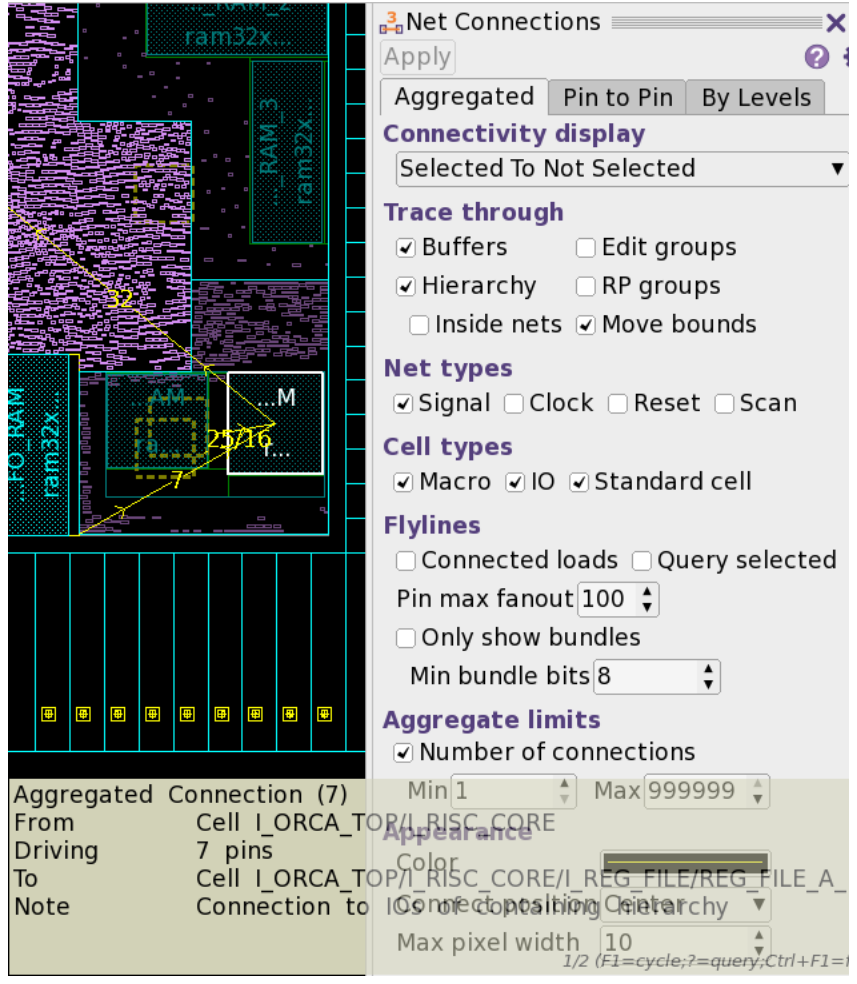
\includegraphics[width=0.92\textwidth]{gui-fig-077.png}
\caption{线网连接飞线面板}
\label{fig:gui-77}
\end{figure}

\subsection{飞线显示模式}
\subsubsection*{Flyline Display Modes}

Net Connections 面板支持下列飞线显示模式：
\begin{itemize}
  \item Aggregated（默认）
  \item Pin to Pin
  \item By Levels
\end{itemize}

这些模式分述如下。使用某一模式时，先单击面板顶部相应的选项卡（Aggregated、Pin to Pin 或 By Levels），再单击 Apply。

\subsection{管脚到管脚飞线}
\subsubsection*{Pin to Pin Flylines}

在 Pin to Pin 模式下，工具为各个管脚（pin）显示飞线。若起始管脚是驱动管脚（driver pin），飞线从每个起始管脚画到全部已追踪的负载管脚（load pin）。若起始管脚是负载管脚，工具则把飞线画到全部已追踪的驱动管脚。

\subsection{按级数}
\subsubsection*{By Levels}

在 By Levels 模式下，工具按 Driver 与 Load 选项所指定的追踪深度显示飞线。除缓冲器单元（buffer）外，工具把每个标准单元计为一级。若选中 \opt{Ignore buffers}，缓冲器不计入级数。此模式还支持为所选驱动管脚与负载管脚使用不同的飞线颜色。

单击一条聚合飞线（aggregated flyline），可以下钻并查看单条飞线的细节。工具打开 Net Connections Explorer 对话框，并显示该聚合飞线所代表的线网列表。Net Connections Explorer 对话框的进一步说明见第~\ref{sec:gui-fly-explorer}~节。要查看单条飞线，也可以取消选中 \opt{Aggregate by block}。取消该选项后，工具用单条飞线替换聚合飞线。

\begin{noteBox}
工具根据路径上所选的管脚以及所选对象的类型来显示飞线。所选管脚是否位于层次边界上，显示的飞线也会不同。
\end{noteBox}

\subsection{聚合飞线}
\subsubsection*{Aggregated Flylines}

在 Aggregated 飞线模式下，工具按飞线驱动管脚与负载管脚的父层次单元、移动约束（move bound）、编辑组（edit group）、相对布局组（RP group）或电压区（voltage area）对这些管脚分组。聚合飞线显示为一条线，并带有负载管脚和（或）驱动管脚的计数。该计数显示在每一对唯一相连父对象的中心。要显示哪些父对象类型，由所选的 Trace through 选项决定。若某类穿越追踪对象未在面板中选中，则仍把它作为一种可能的父对象类型。若最初选中的对象是编辑组、RP 组、移动约束或电压区，则这些对象类型也属于候选父对象类型。

\subsection{设置飞线显示选项}
\subsubsection*{Setting Flyline Display Options}

用 Connectivity Display 选项，按所选对象更改所显示的连接：
\begin{itemize}
  \item \opt{Selected to All}：显示任意选中对象与任何其他对象之间的飞线。
  \item \opt{Selected to Selected}：只显示选中对象之间的飞线。
  \item \opt{Selected to Not Selected}：若只选中一个对象，显示该选中对象与任何其他对象之间的飞线；若选中两个或更多对象，显示从每个并未连接到另一选中对象的选中对象出发的飞线。
\end{itemize}

用 Trace through 选项控制线网如何追踪：
\begin{itemize}
  \item \opt{Buffers}：选中此选项后，继续穿过缓冲器单元追踪，直到到达非缓冲器单元。取消选中后，工具在到达缓冲器单元或任何其他单元时停止追踪。
  \item \opt{Hierarchy}：选中此选项后，继续穿过层次管脚追踪。取消选中后，工具在到达层次管脚时停止追踪。
  \item \opt{Edit groups}：选中此选项后，在编辑组边界处停止追踪。取消选中后，追踪时忽略编辑组。
  \item \opt{RP groups}：选中此选项后，在 RP 组边界处停止追踪。取消选中后，追踪时忽略 RP 组。
  \item \opt{Inside nets}：选中此选项后，追踪块内部的线网。默认追踪块外部的线网。此选项可与 Pin to Pin 选项卡中的 \opt{Through points} 选项组合使用，以便在选中某个块管脚时追踪穿越连接（feedthrough connection）。
  \item \opt{Move bounds}：禁用此选项时，追踪在连接移动约束边界上管脚的线网处停止。当移动约束内部的单元连接到移动约束外部的单元时，即形成该边界。若选中移动约束内部的单元，工具不把飞线追踪到移动约束外部的单元。若选中移动约束外部的单元，工具不把飞线追踪到移动约束内部的单元。默认选中此选项，工具会穿过移动约束继续追踪。
\end{itemize}

用 Net Types 选项指定要追踪的线网类型：\opt{Signal}、\opt{Clock}、\opt{Reset}、\opt{Scan}、\opt{Tie High} 与 \opt{Tie Low}。

用 Cell Types 选项指定要追踪的一种或多种单元类型：宏单元、I/O 或标准单元。

用 Flylines 选项进一步控制显示哪些飞线：
\begin{itemize}
  \item \opt{Connected loads}：选中此选项后，显示两个负载之间的飞线。取消选中后，工具只显示驱动与负载之间的飞线。
  \item \opt{Query selected}：选中此选项后，单击对象时更新 Query 面板。该面板显示当前所显示飞线的源、目标以及连接数量。
  \item \opt{Pin max fanout}：隐藏扇出（fanout）大于指定数值的飞线。
  \item \opt{Only show bundles}：选中此选项后，只显示束信号（bundle）的飞线。
  \item \opt{Min bundle pins}：隐藏管脚数少于指定数值的束的飞线。
\end{itemize}

用 Aggregated Connections 选项按连接数控制聚合飞线的显示：
\begin{itemize}
  \item \opt{Number of connections}：选中此选项后，用 Min 与 Max 设置过滤聚合飞线；若总连接数超出指定范围，则隐藏该聚合飞线。
  \item \opt{Min}：在已选中 \opt{Number of connections} 且总连接数小于指定值时，隐藏该聚合飞线。
  \item \opt{Max}：在已选中 \opt{Number of connections} 且总连接数大于指定值时，隐藏该聚合飞线。
\end{itemize}

用 Include 选项控制所追踪的单元类型：
\begin{itemize}
  \item \opt{Macros}：选中此选项后，追踪中包含宏单元。
  \item \opt{IOs}：选中此选项后，追踪中包含 I/O 单元。
  \item \opt{Standard cells}：选中此选项后，追踪中包含标准单元。
\end{itemize}

用 Appearance 选项控制飞线的宽度与位置：
\begin{itemize}
  \item \opt{Connect Position}：指定飞线起点或终点的绘制位置，可选 center、inside、lower left、lower right、upper left 或 upper right。
  \item \opt{Max pixel width}：把飞线的绘制宽度限制为指定的像素数。
  \item \opt{Nets per pixel}：按线网连接数指定飞线宽度。例如设置为 100 nets/pixel，而某条线网连接含有 300 条连接时，工具绘制 3 像素宽的线（300 条线网 / 每像素 100 条线网 = 3 像素）。
  \item \opt{Color}：指定飞线的颜色。
\end{itemize}

\subsection{显示到布线通道的连接}
\subsubsection*{Displaying Connections to Route Corridors}

选中一条布线通道（route corridor）时，工具取得该布线通道所对应线网的管脚，并从管脚中心向布线通道形状的最近边绘制飞线。若布线通道中含有连接到该布线的中间单元，工具用另一种颜色向这些单元绘制飞线。

\subsection{线网连接浏览器}
\label{sec:gui-fly-explorer}
\subsubsection*{Net Connections Explorer}

使用 Net Connections Explorer 查询聚合飞线中的单条线网，或在单条飞线中显示各条线段网。单击任意飞线即可打开该对话框。对话框显示源块或源单元、目标块或目标单元，以及该飞线所代表的线网列表。可以单击 From: 或 To: 文本后面的名称，以选中对应的块、单元或端口。将指针移到对话框右上角的 Info 图标上，可查看对话框中所显示线网连接的摘要信息。

\begin{figure}[htbp]
\centering
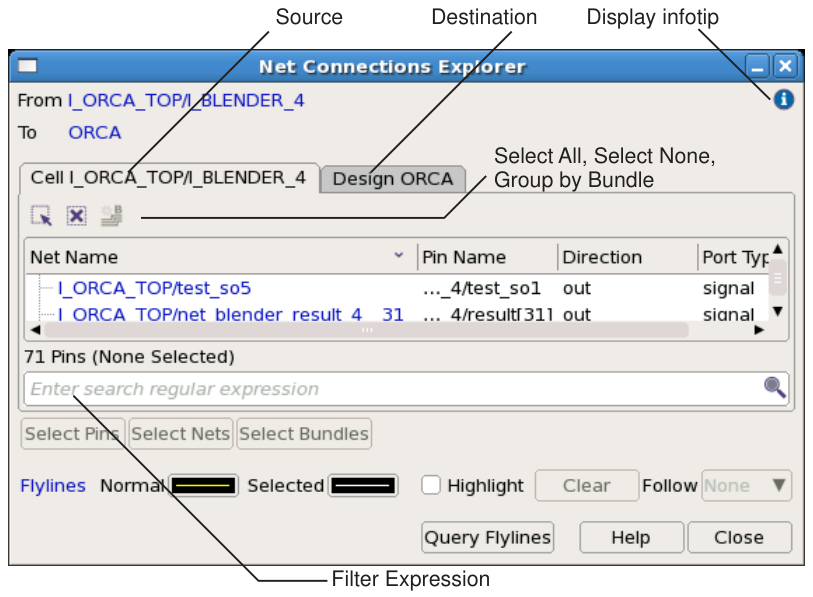
\includegraphics[width=0.92\textwidth]{gui-fig-078.png}
\caption{线网连接浏览器的聚合飞线模式}
\label{fig:gui-78}
\end{figure}

对话框显示两个选项卡：一个选项卡包含源对象的管脚与线网，另一个选项卡包含目标对象的管脚与线网。单击相应选项卡，即可显示与该对象关联的线网和管脚。

要过滤线网列表，在框中输入过滤表达式。表达式可以是简单匹配表达式，也可以是 Tcl 正则表达式。默认把过滤表达式应用于线网名。要对管脚名应用该表达式，使用语法 \cmd{"Pin Name:string"}，其中 \cmd{string} 是搜索表达式，\cmd{Pin Name} 是该列的列标题。

单击 Select Pins 或 Select Nets 按钮，在版图中选中高亮线网的管脚或线网。单击 Select Bundles，选中高亮线网对应的线网束。

要更改未选中飞线或已选中飞线的颜色，单击 Normal 右侧或 Selected 右侧的飞线颜色框。要让先前选中的飞线继续显示在版图中，选中 Highlight。要清除先前显示的飞线，单击 Clear。

用 Follow 设置控制工具如何把所选飞线放到视图中心。要保持同一缩放比例，并把版图平移到使所选飞线位于视图中心，在 Follow 框中选择 Pan。要平移版图并放大，使飞线适合视图，在 Follow 框中选择 Zoom。

追踪单条飞线时，显示如图~\ref{fig:gui-79} 所示。

\begin{figure}[htbp]
\centering
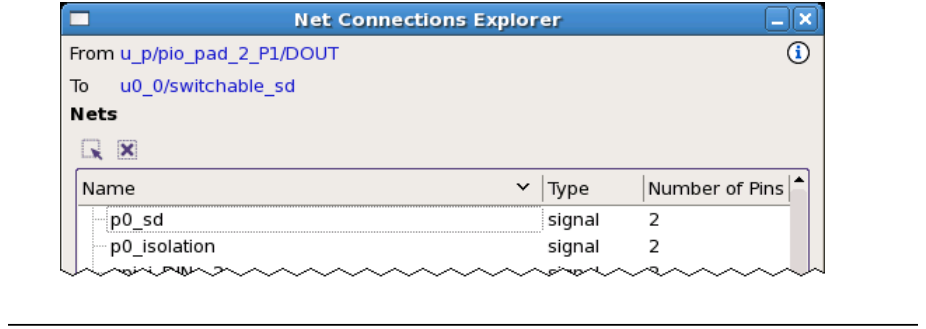
\includegraphics[width=0.92\textwidth]{gui-fig-079.png}
\caption{线网连接浏览器的单条飞线模式}
\label{fig:gui-79}
\end{figure}

要在 Query 面板中显示当前飞线连接列表，单击 Query Flylines。要查看 Net Connections Explorer 对话框的帮助信息，单击 Help。

\section{路径分析器飞线}
\subsection*{Path Analyzer Flylines}

IC Compiler II 工具支持 Path Analyzer Flylines 工具，用于查看设计中顶层信号（top-level signal）、宏单元、端口与层次之间的时序路径连接。使用 Path Analyzer Flylines 工具，可以识别可能与版图有关的时序问题，并交互分析布局对时序的影响。该工具提供两种分析模式，即连接模式（connection mode）与时序模式（timing mode），用来决定飞线优先显示哪些信息。要打开 Path Analyzer Flylines 面板，选择 \textbf{View > Flylines > Path Analyzer Flylines}，或单击 Path Analyzer Flylines 按钮。Path Analyzer Flylines 面板见图~\ref{fig:gui-80}。

\begin{figure}[htbp]
\centering
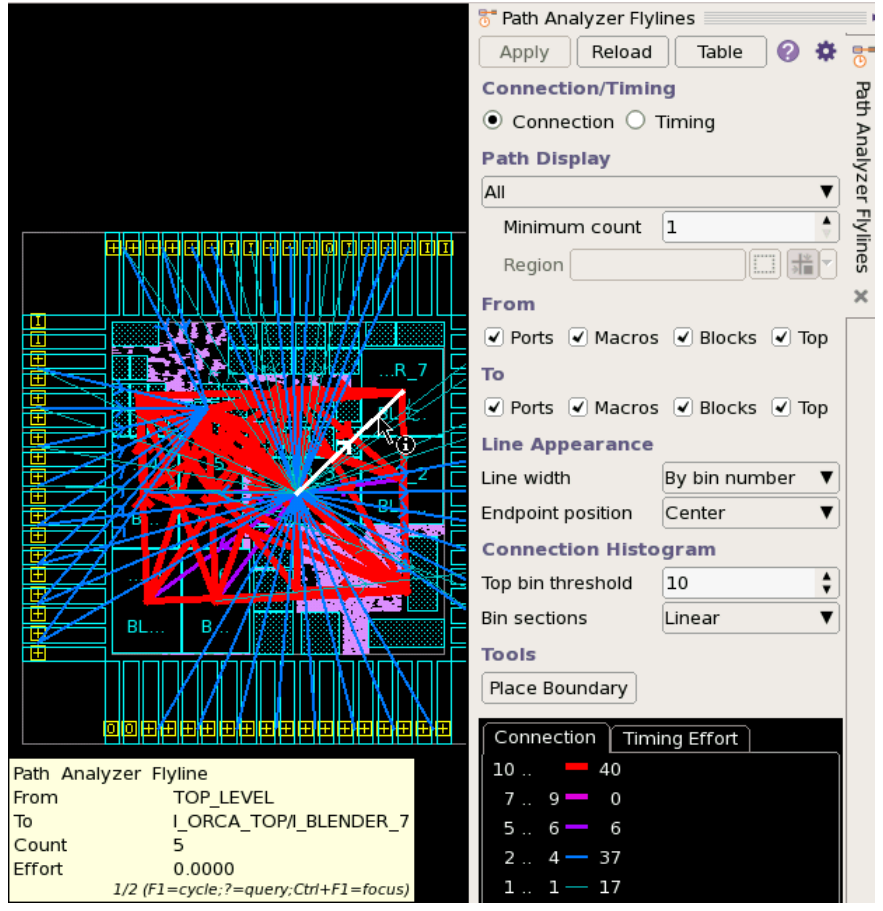
\includegraphics[width=0.92\textwidth]{gui-fig-080.png}
\caption{路径分析器飞线面板}
\label{fig:gui-80}
\end{figure}

单击面板顶部的 Reload 按钮，重新加载飞线。

若版图中含有模块边界（module boundary），单击 Tools 区中的 Place Boundary 按钮，把当前显示的模块边界放到块版图显示上。工具把每个模块边界居中放在该模块标准单元的位置上。工具用画到模块边界的飞线表示与标准单元的连接，模块内部所含的宏单元与层次块不参与这一表示。与宏单元的连接用直接连到宏单元的飞线表示，而不连到模块边界。若某个模块不含标准单元，模块边界放在坐标 (0,0)，并且不向该模块边界绘制飞线。

模块边界提供设计层次中单元物理位置的信息。可以用 Hierarchy Browser 创建模块边界，并与 Path Analyzer Flylines 工具一起使用。当飞线连接到模块边界内的某个单元时，Path Analyzer Flylines 工具把飞线画到模块边界。若不存在模块边界，Path Analyzer Flylines 工具把飞线画到块的中心。要检查层次，选择 \textbf{View > Hierarchy Browser} 启动 Hierarchy Browser 工具。

\subsection{按连接数查看时序路径}
\label{sec:gui-fly-bycount}
\subsubsection*{Viewing Timing Paths by Number of Connections}

单击 Reload 按钮后，Connection/Timing 区中的 Connection 模式默认处于选中状态。Connection 模式显示设计中端口、模块与宏单元之间的时序路径连接飞线。工具按连接数对飞线分档（binning）并分组；连接数最多的飞线显示为红色。若只看到浅蓝色飞线，可在 Line Appearance 区更改 \opt{Threshold for Top Bin} 的值来调整分档。

若看到跨越很长距离的红色或亮紫色飞线，可能需要修改布图规划（floorplan）以缩短这些路径。大量长路径会造成布线拥塞（routing congestion），并在对块做时序分析时加重总负裕量（total negative slack，TNS）问题。

将鼠标指针移到飞线上，可查看更多信息。工具显示信息提示（infotip），如图~\ref{fig:gui-81}；此例中，高亮飞线的全部路径方向相同。信息提示显示路径终点（endpoint）、两个对象之间的飞线计数，以及优化这些路径时序所需的相对时序努力。若该努力大于 1.0，对该路径做时序收敛时可能会遇到困难。

\begin{figure}[htbp]
\centering
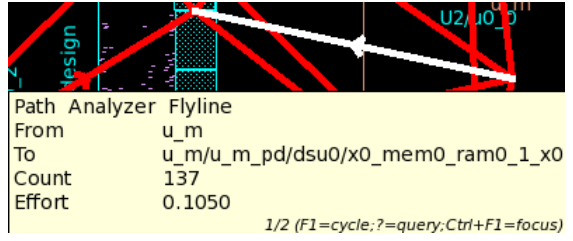
\includegraphics[width=0.92\textwidth]{gui-fig-081.png}
\caption{带信息提示的单向飞线}
\label{fig:gui-81}
\end{figure}

图~\ref{fig:gui-82} 是信号沿两个方向传输的飞线。飞线上不显示方向箭头。信息提示把信号计数显示为 \cmd{Total - (endpoint1 to 2 + endpoint2 to 1)}，把 Effort 显示为 \cmd{Total maximum - max of (endpoint1 to 2 max to endpoint2 to 1 max)}。

\begin{figure}[htbp]
\centering
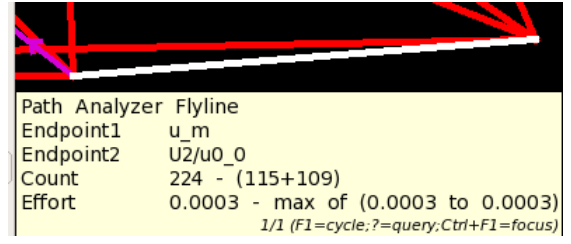
\includegraphics[width=0.92\textwidth]{gui-fig-082.png}
\caption{混合方向的飞线}
\label{fig:gui-82}
\end{figure}

单击飞线可展开该飞线，并查看对象之间的各条连接。工具为每条时序路径显示一条飞线，如图~\ref{fig:gui-83}。要去掉这些细节飞线，另选一个对象，或单击版图外部。

\begin{figure}[htbp]
\centering
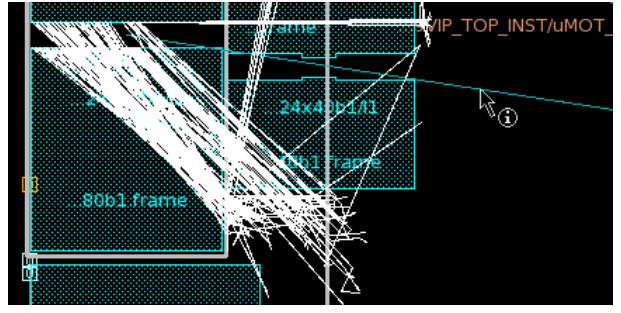
\includegraphics[width=0.92\textwidth]{gui-fig-083.png}
\caption{详细连接飞线}
\label{fig:gui-83}
\end{figure}

若只查看经过设计中某一区域的飞线，在 Path Display 框中选择 Region，并单击图~\ref{fig:gui-84} 所示的虚线方块按钮。用鼠标在版图上绘制矩形，指定分析区域。工具去掉不经过该区域的飞线。

\begin{figure}[htbp]
\centering
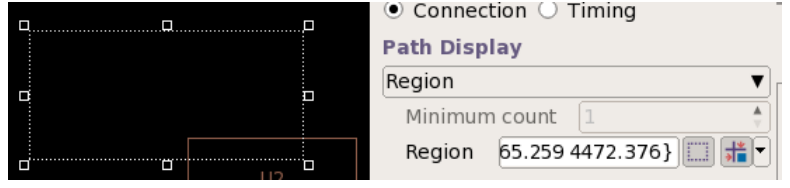
\includegraphics[width=0.92\textwidth]{gui-fig-084.png}
\caption{创建区域矩形}
\label{fig:gui-84}
\end{figure}

过滤飞线的进一步说明见第~\ref{sec:gui-fly-filter}~节。

\subsection{按关键程度查看时序路径}
\subsubsection*{Viewing Timing Paths by Criticality}

在 Connection/Timing 区选择 Timing，显示设计中各对象之间时序最关键路径的时序路径连接飞线。在时序模式下，工具按连接的关键程度（criticality）对飞线分档，并把最关键的飞线显示为红色。按第~\ref{sec:gui-fly-bycount}~节所述，将指针移到飞线上并单击飞线，可查看这些飞线的更多信息。

用 Distance Sensitivity 框控制计算优化努力时对飞线长度所加的权重。更改 Distance Sensitivity 后，工具重新计算该飞线的优化努力。Distance Sensitivity 的值越大，工具对较长飞线所加的权重越大。更新后的努力值可在信息提示中查看。

一般而言，线电阻（wire resistance）较高的工艺可能需要较高的 Distance Sensitivity 设置。若只有在灵敏度很高（7 或更大）时才出现红色飞线，则该设计很可能没有时序问题。

\subsection{更改飞线显示}
\subsubsection*{Changing the Flyline Display}

单击 Display 选项卡，查看并修改 Path Analyzer Flylines 显示的线宽与分档设置。选中 \opt{Apply line widths}，按对象之间的连接数更改飞线线宽。选中 \opt{Log Scale}，把分档改为使用对数刻度（logarithmic scale），而不使用线性刻度（linear scale）。在 \opt{Threshold for Top Bin} 框中输入新值，设置最高档的最大值。

在连接模式下，Display 选项卡用颜色表示每条飞线的相对连接数。若选中 \opt{Apply line widths}，工具用不同线宽显示飞线，最高档使用最宽的线。

在时序模式下，颜色表示时序飞线的关键程度。若选中 \opt{Apply line widths}，工具用不同线宽表示相对连接数，最宽的线表示连接数最多。

\subsection{按设计对象及其他约束过滤}
\label{sec:gui-fly-filter}
\subsubsection*{Filtering by Design Object and Other Constraints}

在 From 与 To 设置区中选中要分析的对象类型。在 Path Display 框中选择一项，指定创建飞线时使用的源对象与目标对象：
\begin{itemize}
  \item \opt{All}：显示飞线，不附加任何选择条件。From 与 To 设置处于启用状态。
  \item \opt{Region}：显示经过用户指定矩形的飞线。From 与 To 设置处于启用状态。
  \item \opt{Selected From/To All}：显示以选中对象为起点或终点、并连到任何其他对象的飞线。From 与 To 设置处于禁用状态。
  \item \opt{Selected to Selected}：显示以选中对象为起点或终点的飞线。From 与 To 设置处于禁用状态。
  \item \opt{All to Selected}：显示从任意对象开始、并在选中对象处结束的飞线。From 与 To 设置处于禁用状态。
  \item \opt{Selected to All}：显示从选中对象开始、并在任何其他对象处结束的飞线。From 与 To 设置处于禁用状态。
\end{itemize}

\subsection{在表中查看时序路径信息}
\subsubsection*{Checking Timing Paths Info in Table}

单击控制板（palette）顶部的 Table 按钮，在表中显示飞线终点、连接计数与时序努力。图~\ref{fig:gui-85} 是一个示例表。

\begin{figure}[htbp]
\centering
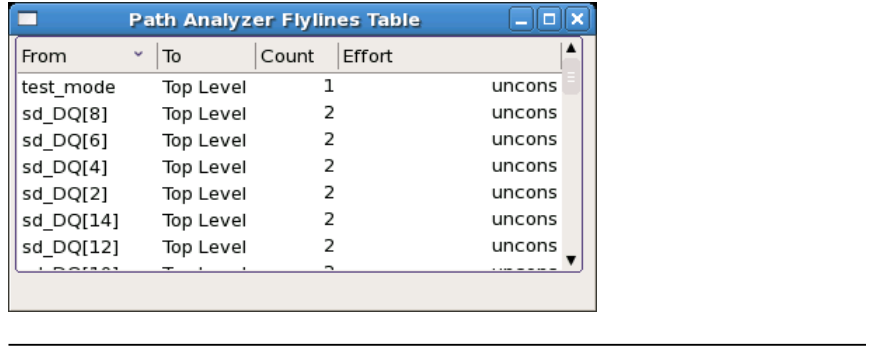
\includegraphics[width=0.92\textwidth]{gui-fig-085.png}
\caption{路径分析器飞线表}
\label{fig:gui-85}
\end{figure}

\subsection{路径分析器飞线最佳实践}
\subsubsection*{Path Analyzer Flylines Best Practices}

使用 Path Analyzer Flylines 工具时，可参考下列建议：
\begin{itemize}
  \item 对大多数应用，应取消选中 From 与 To 区中的 \opt{Top}，以去掉不连接到任何特定宏单元或模块边界的飞线。这样更容易看清其余飞线和其他信息。
  \item 在连接模式下，输入大于零的 \opt{Minimum count} 值，指定对象之间至少要有多少条连接才显示飞线。
  \item 在时序模式下，切换 Path Display 区中的 \opt{Unconstrained}，以包含没有时序约束的时序路径飞线，也就是努力为 0 的路径。切换 \opt{Unachievable}，以包含无法满足当前时序约束的路径飞线，也就是努力为 10 或更大的路径。在 \opt{Minimum Effort} 中输入最低努力级别，以隐藏努力级别小于或等于该指定值的路径。
\end{itemize}

\section{数据流飞线}
\subsection*{Data Flow Flylines}

使用 Data Flow Flylines 工具查看宏单元、块、模块边界与 I/O 端口之间的连接。该工具帮助理解宏单元布局质量，并查看设计中的宏单元到宏单元路径。要打开 Data Flow Flylines 面板，选择 \textbf{View > Flylines > Data Flow Flylines}，或单击 Data Flow Flylines 按钮。

\begin{figure}[htbp]
\centering
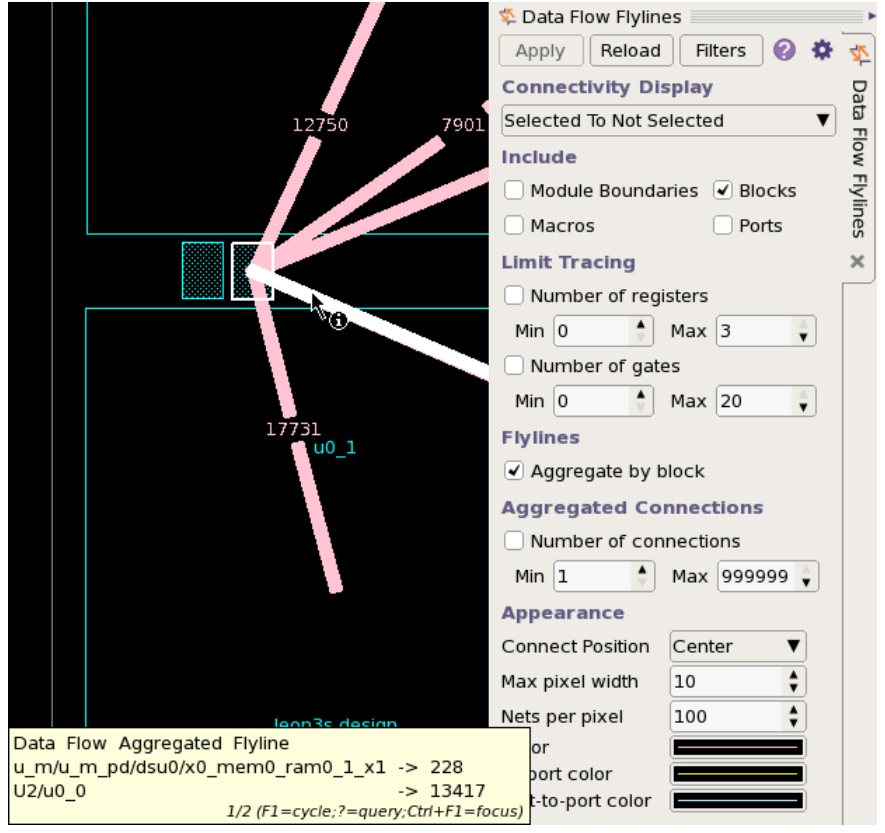
\includegraphics[width=0.92\textwidth]{gui-fig-086.png}
\caption{数据流飞线面板}
\label{fig:gui-86}
\end{figure}

本节包括以下内容：
\begin{itemize}
  \item 计算数据流飞线
  \item 追踪飞线
  \item 设置追踪选项
  \item 查看飞线细节并过滤飞线
  \item 数据流飞线的管脚与线网过滤器
  \item 用 Tcl 命令分析数据流飞线
  \item 保存与恢复数据流飞线连接数据
\end{itemize}

\subsection{计算数据流飞线}
\label{sec:gui-fly-compute}
\subsubsection*{Computing Data Flow Flylines}

追踪飞线之前，必须先计算飞线，以便把它们载入工具，步骤如下：
\begin{enumerate}
  \item 单击 Data Flow Flylines 面板上的 Reload 按钮。
  \item 在 Compute Data Flow Flylines 对话框中，选择要追踪的寄存器（register）级数、门（gate）级数和最大扇出。
  \item 单击 Filters 按钮，指定追踪期间要忽略的线网和管脚。进一步说明见第~\ref{sec:gui-fly-pinnet}~节。
  \item 单击 OK，计算数据流飞线。
\end{enumerate}

\subsection{追踪飞线}
\subsubsection*{Tracing Flylines}

初始化数据流飞线之后，可以在版图窗口中交互追踪飞线。典型流程包括以下步骤：
\begin{enumerate}
  \item 单击某个宏单元、块、模块边界或 I/O 端口以选中它；工具显示到 Include 区中所选对象的飞线连接。
  \item 将指针移到飞线上，在信息提示中查看连接数。
  \item 单击该飞线，打开 Data Flow Connections and Filters 对话框。对话框显示该飞线所代表的连接列表，进一步说明见第~\ref{sec:gui-fly-details}~节。
  \item 单击列表中的一条路径，显示该路径的飞线。
  \item 单击 ([+]) 按钮展开该路径，再单击代表路径中某一段的一行；工具用红色显示该段的详细路径飞线。
  \item 继续单击路径中的其他段进行追踪，或按上箭头键或下箭头键，在段列表中滚动。
\end{enumerate}

\subsection{设置追踪选项}
\subsubsection*{Setting Tracing Options}

Data Flow Flylines 工具提供控制飞线追踪的选项。用 Connectivity Display 设置控制显示哪些连接：
\begin{itemize}
  \item \opt{All}：显示全部路径。
  \item \opt{Selected To All}：显示从选中对象到全部相连对象的路径。
  \item \opt{Selected To Selected}：显示从选中对象到其他已连接的选中对象的路径。
  \item \opt{Selected To Not Selected}：显示从选中对象到已连接但未被选中的对象的路径。
\end{itemize}

用 Include 区选择追踪时要包含的对象类型。

用 Limit Tracing 区调整飞线中包含的寄存器数量和门数量。只能在 Compute Data Flow Flylines 对话框里已指定的级数之内减少级数；要增加可用级数，单击 Reload 并重新计算飞线。

\begin{noteBox}
默认情况下，源管脚与目标管脚之间最小门数和最大门数的计数不包含缓冲器与反相器（inverter）。因此，详细路径连接所显示的门数可能多于预期。
\end{noteBox}

聚合连接是把源对象与目标对象相同的飞线合并为一条飞线。要更改聚合飞线的行为：
\begin{itemize}
  \item 选中或取消选中 \opt{Aggregate}，以显示聚合飞线或显示单条飞线。
  \item 选中 \opt{Number of connections}，并为聚合飞线选择最小连接数与最大连接数；连接数超出该范围的聚合飞线会被工具隐藏。
\end{itemize}

用 Appearance 区更改飞线的连接点、线宽和颜色：
\begin{itemize}
  \item 在列表中选择一项 \opt{Connect Position}，更改飞线在版图中的绘制位置；工具把飞线画到对象上的指定位置。
  \item 用 \opt{Max pixel width} 设置把飞线的绘制宽度限制为指定的像素数。
  \item 用 \opt{Nets per pixel} 设置按线网连接数指定飞线宽度。例如设置为 100 nets/pixel，而某条线网连接含有 300 条连接时，得到 3 像素宽的线（300 / 100 = 3）。
  \item 用 \opt{Color} 设置更改宏单元、块与模块边界之间飞线的显示颜色。
  \item 用 \opt{To port color} 设置更改连到端口的飞线颜色。
  \item 用 \opt{Port-to-port color} 设置更改端口到端口飞线的颜色。
  \item Wire length 是所选对象的飞线总长度，由工具自动计算。
\end{itemize}

\subsection{查看飞线细节并过滤飞线}
\label{sec:gui-fly-details}
\subsubsection*{Viewing Flyline Details and Filtering Flylines}

使用 Data Flow Connections and Filters 对话框，查看聚合飞线内部的各条连接、查看单条飞线，或设置追踪飞线时使用的管脚过滤器与线网过滤器。要打开此对话框，单击 Data Flow Flylines 工具生成的聚合飞线。

\begin{noteBox}
创建过滤器之后，必须在 Data Flow Flylines 面板中单击 Reload，重新计算飞线并应用该过滤器。
\end{noteBox}

\begin{figure}[htbp]
\centering
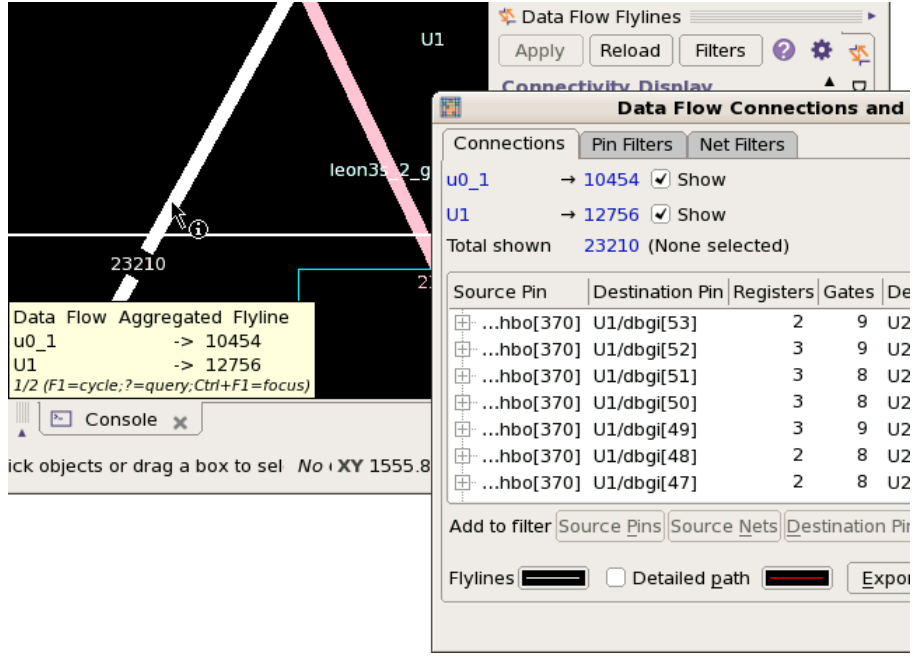
\includegraphics[width=0.92\textwidth]{gui-fig-087.png}
\caption{数据流连接与过滤器}
\label{fig:gui-87}
\end{figure}

Connections 选项卡显示所选飞线内部的连接列表。在该选项卡顶部，工具显示飞线所连接的两个对象的名称，以及从任一对象发出的连接数。若两个对象之间两个方向都有连接，单击对象名右侧的 Show 按钮，把从该对象发出的连接加入列表，或从列表中去掉。

用 Connections 选项卡追踪飞线：
\begin{enumerate}
  \item 单击列表中的一条路径；工具显示该路径的飞线。
  \item 选中 \opt{Detailed path}，显示路径中的全部中间连接；工具为每一段管脚到管脚的连接显示一条红色飞线。
  \item 单击 Source Pins、Source Nets、Destination Pins 或 Destination Nets 按钮，把所选路径复制到相应过滤器；要应用这些过滤器，必须单击 Reload 重新计算飞线。
  \item 单击 ([+]) 按钮展开路径，显示中间连接的源管脚与目标管脚。
  \item 单击列表中代表路径某一段的一项；工具用红色显示该段的详细路径飞线。
  \item 按上箭头键或下箭头键滚动路径，并在版图中高亮不同的段。
  \item 按住鼠标按钮并沿列表向下拖动指针，把路径中的其他段加入选择。
\end{enumerate}

\begin{figure}[htbp]
\centering
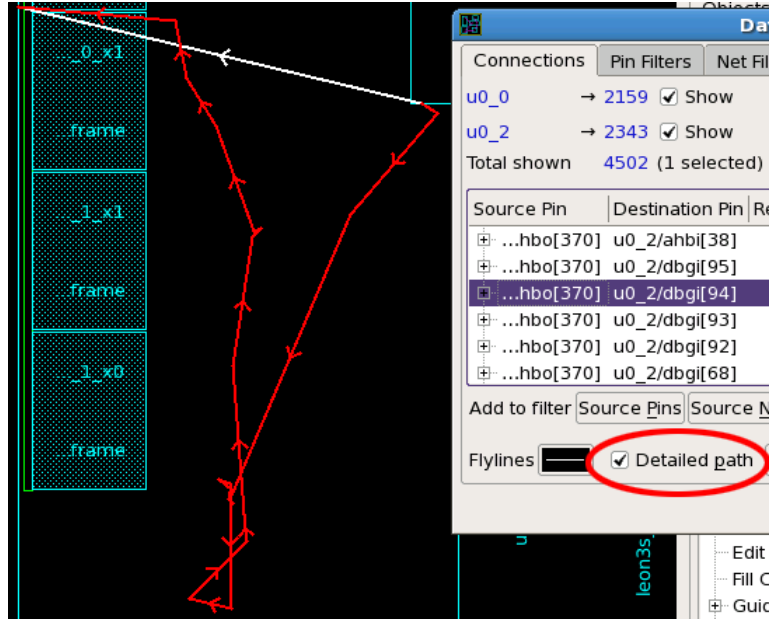
\includegraphics[width=0.92\textwidth]{gui-fig-088.png}
\caption{飞线与详细路径}
\label{fig:gui-88}
\end{figure}

为提高性能，工具可能不会载入全部路径细节。此时，工具在 Detailed Path 列中显示消息 \cmd{Path is not loaded. Double-click to load.}。可以双击该路径以载入它，或单击 Load All Paths 按钮，载入其余全部尚未载入的路径。

要保存列表中各路径的源管脚、目标管脚、寄存器数和门数，并以逗号分隔，单击 Export 按钮。

\subsection{数据流飞线的管脚与线网过滤器}
\label{sec:gui-fly-pinnet}
\subsubsection*{Data Flow Flylines Pin and Net Filters}

要打开 Data Flow Connections and Filters 对话框，单击 Data Flow Flylines 面板中的 Filters 按钮。Pin Filters 与 Net Filters 选项卡包含飞线追踪期间要忽略的管脚列表和线网列表。要向列表添加一项，在 Patterns 框中输入名称并单击 Add。也可以输入与 \cmd{get\_pins} 或 \cmd{get\_nets} 命令兼容的表达式，以指定一个或多个管脚或线网。

在 Pin Filters 或 Net Filters 选项卡中，用右侧按钮修改列表：
\begin{itemize}
  \item 用 Add Selected Pins 按钮或 Add Selected Nets 按钮，把版图中选中的管脚或线网加入列表。
  \item 用 Add Pins of Selected 按钮或 Add Nets of Selected 按钮，加入所选对象的全部管脚或线网。
  \item 用 Remove 按钮从列表中去掉选中项。
  \item 用 Remove All 按钮清空列表。
  \item 用 Write to File 按钮把管脚或线网列表写入文件，每行一项。
  \item 用 Read from File 按钮从文件载入管脚或线网列表。
\end{itemize}

\subsection{用 Tcl 命令分析数据流飞线}
\subsubsection*{Using Tcl Commands to Analyze Data Flow Flylines}

在 Data Flow Flylines 面板中单击 Reload 按钮时，工具打开 Compute Data Flow Flylines 对话框，并提示输入要追踪的级数和最大扇出。也可以直接使用 \cmd{compute\_dff\_connections} Tcl 命令，并向该命令指定选项，以生成寄存器追踪信息。例如，下面的 \cmd{compute\_dff\_connections} 命令生成路径信息，并指定追踪两级寄存器、15 级门，以及最大扇出数为 50。

\begin{lstlisting}
icc2_shell> compute_dff_connections -max_reg 2 -max_gate 15 \
   -max_fanout 50
\end{lstlisting}

用 \cmd{compute\_dff\_connections} 命令追踪飞线之后，使用 \cmd{get\_dff\_connections} 命令返回全部路径，或只返回满足指定条件的路径。默认情况下，该命令返回由 \cmd{compute\_dff\_connections} 命令生成的全部路径的集合。

\begin{noteBox}
用 \opt{-max\_reg} 与 \opt{-max\_gate} 指定的值必须小于或等于 \cmd{compute\_dff\_connections} 命令中对应选项所指定的值。
\end{noteBox}

下面的示例返回由 \cmd{compute\_dff\_connections} 命令提取的特定路径，并返回单条路径的属性。

\begin{itemize}
  \item 返回全部路径。
\begin{lstlisting}
icc2_shell> get_dff_connections
\end{lstlisting}
  \item 返回不含寄存器且不含门的路径。
\begin{lstlisting}
icc2_shell> get_dff_connections -max_reg 0 -max_gate 0
\end{lstlisting}
  \item 返回到达 \cmd{pad[0]} 端口、从 \cmd{pad[0]} 端口出发，以及经过 \cmd{pad[0]} 端口的全部路径。
\begin{lstlisting}
icc2_shell> get_dff_connections -to pad[0]
icc2_shell> get_dff_connections -from pad[0]
icc2_shell> get_dff_connections -through pad[0]
\end{lstlisting}
  \item 返回经过 \cmd{pad[0]} 与 \cmd{u1/u2/o1} 端口的全部路径。
\begin{lstlisting}
icc2_shell> get_dff_connections -through pad[0] -through u1/u2/o1
\end{lstlisting}
  \item 查看集合中单条路径所返回的 \cmd{start.full\_name}、\cmd{end.full\_name} 以及其他属性。
\begin{lstlisting}
icc2_shell> set paths [get_dff_connections -from {pad[6]}]
{{pad[6]::I_ORCA_TOP/I_CONTEXT_MEM ...
icc2_shell> set path [index_collection $paths 0]
{{pad[6]::I_ORCA_TOP/I_CONTEXT_MEM/I_CONTEXT_RAM_0_1/A1[0]}}
icc2_shell> get_attribute $path start.full_name
pad[6]
icc2_shell> get_attribute $path end.full_name
I_ORCA_TOP/I_CONTEXT_MEM/I_CONTEXT_RAM_0_1/A1[0]
icc2_shell> get_attribute $path name
pad[6]::I_ORCA_TOP/I_CONTEXT_MEM/I_CONTEXT_RAM_0_1/A1[0]
icc2_shell> get_attribute $path registers
0
icc2_shell> get_attribute $path gates
10
\end{lstlisting}
\end{itemize}

\subsection{保存与恢复数据流飞线连接数据}
\subsubsection*{Saving and Restoring Data Flow Flylines Connection Data}

退出会话时，工具不保存数据流飞线的连接信息。若希望在以后的会话中使用同一份数据，可以把该信息保存到文件。也可以从已保存的文件中载入，以恢复先前保存的数据流飞线连接信息。

要保存活动视图（active view）当前的数据流飞线连接信息：
\begin{enumerate}
  \item 确认已经计算飞线并载入工具。进一步说明见第~\ref{sec:gui-fly-compute}~节。
  \item 计算飞线之后，用 \cmd{write\_dff\_connections} 命令把数据流飞线连接信息写到文件。
\end{enumerate}

在下面的示例中，工具把数据写到名为 \cmd{dfffile} 的文件。\opt{-force} 选项会覆盖任何同名的已有文件。

\begin{lstlisting}
icc2_shell> write_dff_connections -force -filename dfffile
\end{lstlisting}

要恢复先前保存的数据流飞线连接信息，使用 \cmd{read\_dff\_connections} 命令。

在下面的示例中，工具从名为 \cmd{dfffile} 的文件读取数据流飞线连接信息。

\begin{lstlisting}
icc2_shell> read_dff_connections -filename dfffile
\end{lstlisting}

\begin{itemize}
  \item 将 \opt{-threshold} 选项与 \cmd{read\_dff\_connections} 命令一起使用，以避免当前网表与所要读取的数据流飞线连接不一致时可能出现的问题。该选项的进一步说明见命令手册页。
  \item 若指定文件不在当前工作目录中，工具显示错误消息。
\end{itemize}

若不存在相应附件，将发出 FILE-013 错误。

\begin{lstlisting}
Error: Cannot open file 'filename' for read. (FILE-013)
\end{lstlisting}

要从系统中去掉数据流飞线连接信息文件，使用 \cmd{remove\_dff\_connection\_files} 命令。

在下面的示例中，工具去掉名为 \cmd{dfffile} 的数据流飞线连接文件。要跳过任何消息并以安静模式运行，对该命令使用 \opt{-quiet} 选项。

\begin{lstlisting}
icc2_shell> remove_dff_connection_files -filename dfffile
\end{lstlisting}

\section{寄存器追踪飞线}
\subsection*{Register Tracing Flylines}

IC Compiler II 工具提供 Register Tracing Flylines 工具，用于显示设计中层次、宏单元与端口之间的寄存器连接。可用该工具查看对象之间寄存器连接的飞线，按寄存器级数或扇出限制追踪，显示相连的管脚与端口，并列出路径中的寄存器。要打开 Register Tracing Flylines 面板，选择 \textbf{View > Flylines > Register Tracing}，或单击 Register Tracing Flylines 按钮。Register Tracing Flylines 面板见图~\ref{fig:gui-89}。

\begin{figure}[htbp]
\centering
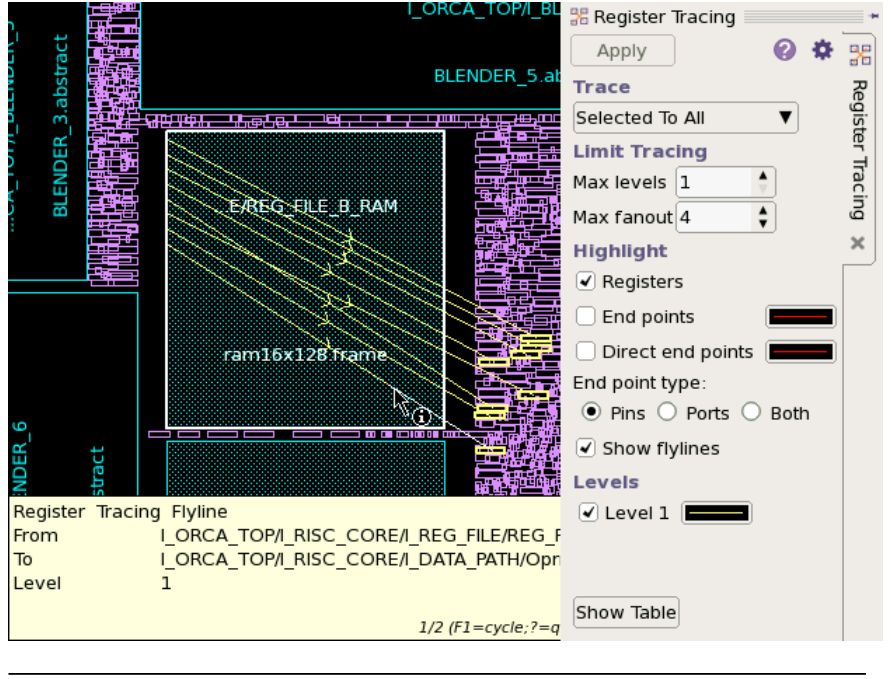
\includegraphics[width=0.92\textwidth]{gui-fig-089.png}
\caption{寄存器追踪飞线面板}
\label{fig:gui-89}
\end{figure}

\subsection{显示飞线}
\subsubsection*{Displaying Flylines}

Register Tracing Flylines 工具在驱动寄存器管脚与接收寄存器管脚之间，为满足指定条件的线网显示飞线。可以按下述方式更改面板中的设置，并单击 Apply 按钮提交更改，从而改变所显示的飞线。
\begin{itemize}
  \item \opt{Trace Selected to All}：按指定级数追踪输出端口，并显示飞线。
  \item \opt{Trace Selected to Selected}：追踪选中对象之间的连接，并显示终点位于其中一个选中对象中的连接。
  \item \opt{Trace All to Selected}：把所有可能的端口和宏单元管脚追踪到所选对象，并且只显示终点位于所选对象中的连接。
  \item \opt{Limit Tracing Max levels}：设置要追踪的最大寄存器级数。
  \item \opt{Limit Tracing Max fanout}：指定停止追踪的扇出级别。
  \item \opt{Highlight registers}：显示并高亮属于寄存器的单元。
  \item \opt{Highlight End points}：以指定的高亮颜色显示并高亮寄存器和端口。
  \item \opt{Highlight Direct End points}：显示并高亮由源管脚（source pin）直接驱动的终点。
  \item \opt{End point type Pins}：只把管脚当作终点。
  \item \opt{End point type Ports}：只把端口当作终点。
  \item \opt{End point type Both}：把管脚和端口都当作终点。
  \item \opt{Show flylines}：切换飞线的可见性。
  \item \opt{All Levels}：切换直到 Limit Tracing 区中所设最大级数的全部追踪级别的可见性。
  \item \opt{Level 1} 等：切换指定级别的可见性。
  \item \opt{Show Table}：显示一个对话框，其中列出满足追踪条件的起点（startpoint）、终点和中间寄存器。单击列表中的一行，在版图中显示对应飞线。单击 Export，把该列表写出。
\end{itemize}

\section{时钟主干规划飞线}
\subsection*{Clock Trunk Planning Flylines}

IC Compiler II 工具提供 Clock Trunk Planning Flylines 工具，用于查看并修改设计中时钟信号的时钟主干（clock trunk）。可用该工具查看各条时钟主干、添加缓冲器、删除缓冲器、检查并修复时钟主干违例，以及为所显示的时钟主干下推（push down）单元。时序信息，例如最差负裕量（worst negative slack，WNS）、TNS 以及其他参数，可以通过为设计中不同的时钟主干规划飞线显示信息提示来查看。要打开 Clock Trunk Planning Flylines 面板，从菜单选择 \textbf{View > Flylines > Clock Trunk Planning}，或单击 Clock Trunk Planning 按钮。Clock Trunk Planning Flylines 面板见图~\ref{fig:gui-90}。

\begin{figure}[htbp]
\centering
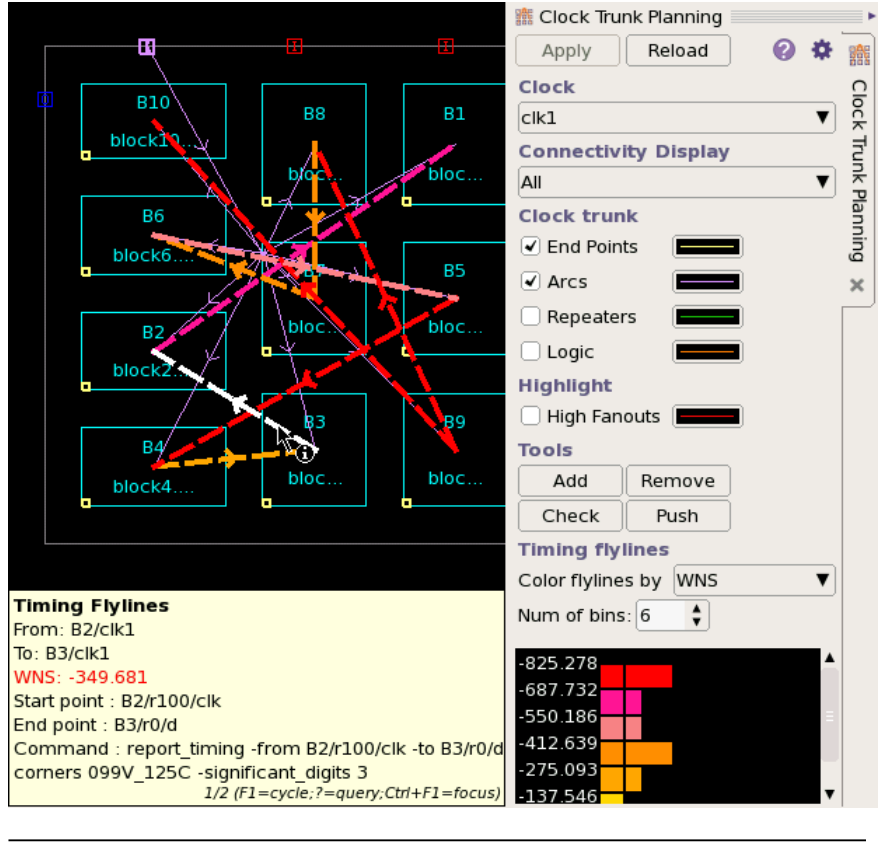
\includegraphics[width=0.92\textwidth]{gui-fig-090.png}
\caption{时钟主干规划控制板}
\label{fig:gui-90}
\end{figure}

\subsection{加载时钟数据}
\subsubsection*{Loading Clock Data}

要把时钟信息载入 Clock Trunk Planning 工具：
\begin{enumerate}
  \item 单击 Reload 按钮。
  \item 在图~\ref{fig:gui-91} 所示的 Reload clock trunk planning 对话框中，选择要加载的时钟。
  \begin{itemize}
    \item 选择 Automatic，加载全部时钟主干。
    \item 选择 Specified，从列表中选择一条或多条时钟主干。按住 Ctrl 键并单击，把时钟加入列表；或按住 Shift 键并单击，一次加入多条时钟。
  \end{itemize}
  \item 单击 OK。
\end{enumerate}

\begin{figure}[htbp]
\centering
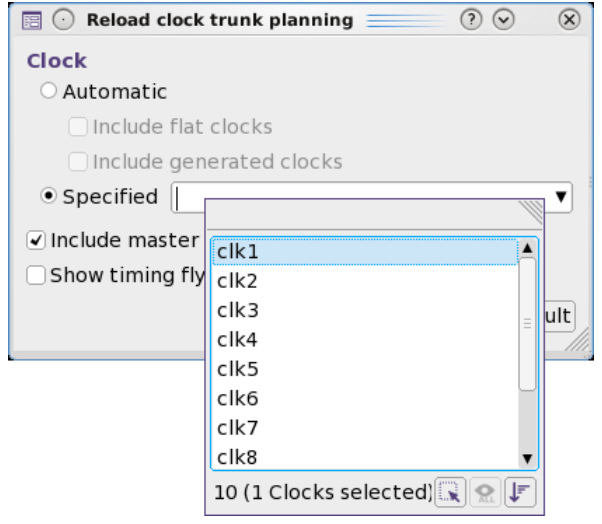
\includegraphics[width=0.92\textwidth]{gui-fig-091.png}
\caption{重新加载对话框}
\label{fig:gui-91}
\end{figure}

工具载入指定的时钟主干。若选择了 Automatic，或选中了多个时钟信号，工具会选中其中一个信号并显示它。要更改所显示的时钟主干，从 Clock 下拉列表中另选一个时钟信号。

\subsection{更改时钟主干高亮}
\subsubsection*{Changing Clock Trunk Highlighting}

用 Clock trunk 区中的控件更改版图里时钟主干元素的颜色。选中元素名旁边的框，即可在版图中显示该元素。单击元素名旁边的色条，并从列表中选择一种颜色，即可更改该时钟主干元素的颜色。
\begin{itemize}
  \item \opt{End Points}：定义时钟终点的颜色。
  \item \opt{Arcs}：定义时钟原点（clock origin）与时钟缓冲器或块之间飞线的颜色。
  \item \opt{Repeaters}：定义中继器（repeater）单元的颜色。
  \item \opt{Logic}：定义逻辑单元的颜色。
  \item \opt{High Fanouts}：定义高扇出线网的颜色。
\end{itemize}

\subsection{添加与删除时钟主干单元}
\subsubsection*{Adding and Removing Clock Trunk Cells}

要在时钟主干上插入时钟缓冲器单元：
\begin{enumerate}
  \item 在控制板的 Clock 框中，选择要插入缓冲器的那条时钟信号的时钟主干。
  \item 在版图中选择要插入缓冲的端口、单元或管脚。该对象必须位于当前选中的时钟主干上。
  \item 单击 Add 按钮。
  \item 在图~\ref{fig:gui-92} 所示的对话框中，选择要插入缓冲的管脚：源管脚、漏管脚（sink pin），或两者都选。
  \item 选中 \opt{Allow on top of blocks} 按钮，允许工具在缓冲器与块重叠时仍然插入缓冲器。
  \item 单击 Add buffer。
\end{enumerate}

工具对第 4 步中所选的每个管脚应用 \cmd{create\_clock\_buffer} 命令，插入一个时钟缓冲器单元。

\begin{figure}[htbp]
\centering
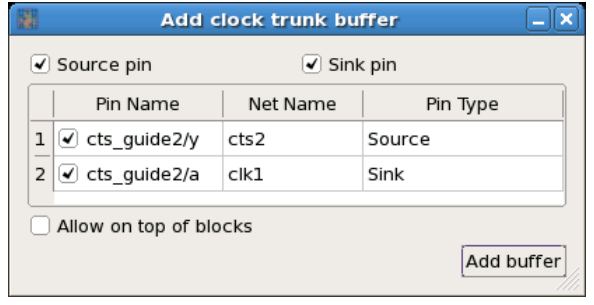
\includegraphics[width=0.92\textwidth]{gui-fig-092.png}
\caption{添加时钟主干缓冲器}
\label{fig:gui-92}
\end{figure}

要去掉一个或多个时钟缓冲器单元：
\begin{enumerate}
  \item 在版图中选中这些单元。
  \item 单击 Remove 按钮。
\end{enumerate}

\subsection{显示块之间的时序飞线}
\subsubsection*{Displaying Timing Flylines Between Blocks}

Clock Trunk Planning 工具可以显示设计中块之间的时序飞线。在控制板底部附近 Timing flylines 区的 Color flylines by 框中，选择一种时序度量：WNS、WNS(OCV)、TNS、Slack、Slack(OCV)、Paths 或 VioPaths\&TNS。其中 OCV 为片上变异（on-chip variation），Slack 为裕量（slack）。工具对路径分档，按档把飞线加到版图上，并在控制板底部显示数值直方图（histogram）。要更改所显示的档数，在 Num of bins 框中设置新值。

要从版图中去掉时序飞线，在 Color flylines by 框中选择 None。

% 第 6 章 Using Map and Visual Modes
\bichapter{使用 Map 与 Visual 模式}{Using Map and Visual Modes}
\label{chap:gui-map}

IC Compiler II GUI 提供一组工具，把设计数据以叠加（overlay）形式显示在版图（layout）上。使用 map mode（Map 模式）与 visual mode（Visual 模式），可以快速找出设计中的问题区域、进行修正，并评估修复效果。

下列主题说明 GUI 所支持的 map mode：
\begin{itemize}
  \item Map 模式概述
  \item 全局布线拥塞图
  \item 通道拥塞图
  \item 单元、管脚、块管脚与功耗密度图
  \item 有效电压区域图
  \item 有效站点阵列图
  \item 线利用率图
  \item 导出与导入 Map 数据
  \item Visual 模式概述
  \item 快照 Visual 模式
  \item 高亮 Visual 模式
  \item 时钟树 Visual 模式
  \item 扫描链 Visual 模式
  \item 区域内线网连接 Visual 模式
  \item 相对布局（RP）组 Visual 模式
  \item 相对布局（RP）线网连接 Visual 模式
  \item 层次 Visual 模式
  \item 单元裕量 Visual 模式
  \item 导入路径管脚 Visual 模式
  \item 电压区域 Visual 模式
\end{itemize}

\section{Map 模式概述}
\subsection*{Map Mode Overview}

Map mode 是分析工具，用来在活动版图视图（layout view）中突出特定的布图规划（floorplan）、布局（placement）或布线（routing）结果。启用某个 map mode 后，GUI 会淡化版图视图中的可见对象，并打开 Map Mode 面板。要在活动版图视图中显示或隐藏某个 map mode，可以选择 \textbf{View > Map}，再选择一种 map mode；也可以单击工具栏上的 map mode 按钮。活动 map mode 的名称出现在 Map Mode 面板顶部的列表中，如图~\ref{fig:gui-93} 所示。全局布线拥塞图见图~\ref{fig:gui-94}。

\begin{figure}[htbp]
\centering
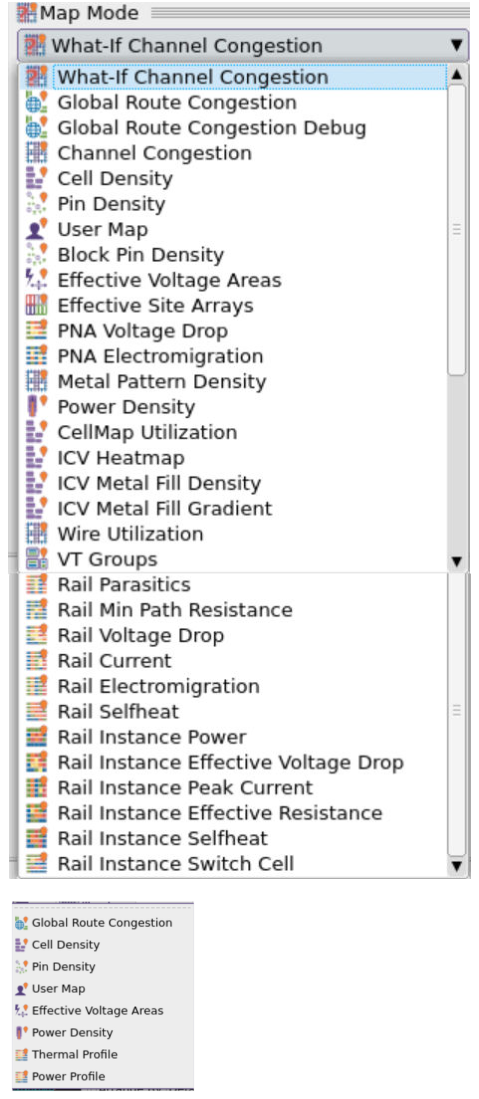
\includegraphics[width=0.92\textwidth]{gui-fig-093.png}
\caption{Map 模式}
\label{fig:gui-93}
\end{figure}

\begin{figure}[htbp]
\centering
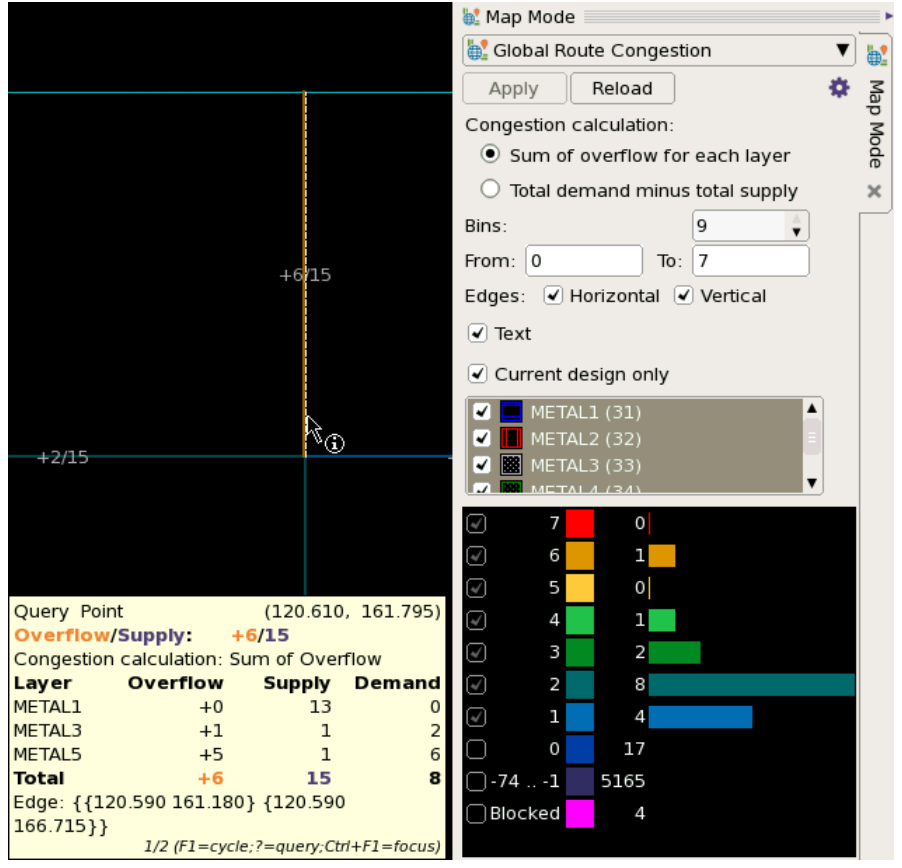
\includegraphics[width=0.92\textwidth]{gui-fig-094.png}
\caption{全局布线拥塞图}
\label{fig:gui-94}
\end{figure}

\subsection{配置直方图}
\subsubsection*{Configuring the Histogram}

在 map mode 面板底部，工具显示当前 map mode 的数值直方图（histogram）。首次生成直方图时必须单击 Reload。要修改直方图：
\begin{itemize}
  \item 选中或取消条形左侧的复选框，即可在版图中显示或隐藏直方图条及其对应数据；也可以在该行任意位置右键，选择 Show 或 Hide。还可以选择 Show all 或 Hide all，以显示或隐藏全部直方图条。
  \item 在该行任意位置右键并选择 Set Style，可更改直方图条以及版图中对应网格的颜色。
  \item 在该行任意位置右键并选择 Configure，可更改其他显示选项；详见「配置 Map 选项」。
\end{itemize}

单击 Apply，按新设置更新 map。

\begin{itemize}
  \item 选择 Show in List，并在 Map Data 对话框中单击某一行，即可定位到设计版图中的特定网格。
\end{itemize}

\begin{figure}[htbp]
\centering
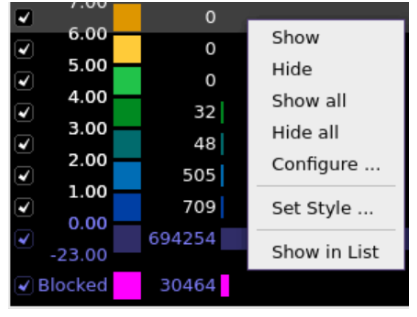
\includegraphics[width=0.92\textwidth]{gui-fig-095.png}
\caption{Map 模式直方图}
\label{fig:gui-95}
\end{figure}

\subsection{更改透明度}
\subsubsection*{Changing the Transparency}

可以用工具 GUI 中的 Alpha 控件调节 map 的透明度（transparency）。也可以对 \cmd{gui\_get\_map\_option}、\cmd{gui\_get\_map\_option\_list} 与 \cmd{gui\_set\_map\_option} 命令使用 \opt{-option} \cmd{alpha}。

下表说明部分设置如何影响 map 的透明度。

\begin{table}[htbp]
\centering
\caption{透明度控制设置}
\begin{tabularx}{\textwidth}{@{}l X@{}}
\toprule
Alpha 设置 & 透明度 \\
\midrule
100\% & 默认（Default），不透明（Opaque） \\
50\% & \\
Off & 完全透明（Fully transparent） \\
\bottomrule
\end{tabularx}
\end{table}

下面的例子用 \cmd{gui\_set\_map\_option} 命令设置透明度。
\begin{lstlisting}
icc2_shell> gui_set_map_option -map cellDensityMap -option alpha -value 10%
\end{lstlisting}

要取回设置，可以使用 \cmd{gui\_get\_map\_option} 命令。例如：
\begin{lstlisting}
icc2_shell> gui_get_map_option -map cellDensityMap -option alpha
\end{lstlisting}

\subsection{配置 Map 选项}
\subsubsection*{Configuring Map Options}

单击 Show Options 按钮并选择 configure，可以对每种 map mode 做进一步配置：
\begin{itemize}
  \item 夸张方案（exaggeration scheme）：设置 Top、Middle 与 Bottom 值，以指定 map mode 与 visual mode 中的颜色夸张方案。这些值设定在版图中显示拥塞条时使用的最小、中位与最大像素数。
  \item Show styles：显示或隐藏直方图中的色标方块。
  \item Show exaggeration：在每条直方图条旁显示或隐藏计算出的夸张值。
  \item Show counts：显示或隐藏每个直方图分档（bin）的边数。
  \item Show histogram：显示或隐藏直方图条。
  \item Show only visible bins in histogram：选中后，仅当该分档的复选框被选中时才显示对应的直方图条。
\end{itemize}

\section{全局布线拥塞图}
\subsection*{Global Route Congestion Map}

IC Compiler II 支持全局布线拥塞图（Global Route Congestion map），用来突出设计中对全局布线（global route）需求很高的区域。拥塞（congestion）区域可能在详细布线（detail route）期间引发问题。要显示全局布线拥塞图，选择 \textbf{View > Map > Global Route Congestion}，或单击 Global Route Congestion 按钮。

要生成全局布线拥塞图，单击 Reload 按钮。工具会显示一个对话框，其中给出用于生成 map 数据的 \cmd{route\_global} 命令及其选项。单击 OK 运行该命令。完成后，工具显示拥塞图。

工具显示拥塞图之后，把指针移到版图窗口并放大，以便更细致地查看 map。把指针移到拥塞条上，可在信息提示（infotip）中查看更多信息。

\subsection{细化全局布线拥塞图}
\subsubsection*{Refining the Global Route Congestion Map}

可以修改 Global Route Congestion Map 面板中的设置，以改变拥塞图的显示方式。使用下列设置更改拥塞图：
\begin{itemize}
  \item Rule level：选择拥塞计算所采用的规则级别。
  \item Congestion calculation：选择 Sum of overflow for each layer 或 Total demand minus total supply，以指定计算拥塞的方法。该设置如何影响显示，见「拥塞图计算」。
  \item Bins：更改 Bins 的值，以改变显示 map 所用的唯一分档数目。分档越多，map 被划分成的取值范围就越多。
  \item From: 与 To:：更改这两个值，以改变 map 与直方图中显示的溢出（overflow）值范围。这些值表示布线单元（route cell）上布线容量的溢出，数值越大表示拥塞越严重。
  \item Edges：选择要显示拥塞值的全局布线单元（global route cell）的边，即 Horizontal 与 Vertical。
  \item Text：选择此项后，在版图中显示一个代表计算出的拥塞值的数字。若看不到这些值，必须放大查看，并确认直方图中已选中相应范围。
  \item Hierarchical：选择此项后，在层次块内部显示拥塞图。
  \item Layers：选择计算拥塞时要考虑的布线层。
\end{itemize}

在面板底部，工具显示拥塞值的直方图。生成 map 之后，可以这样修改直方图：
\begin{itemize}
  \item 选中或取消各层，使它们纳入或排除在拥塞计算之外。
  \item 选中或取消条形左侧的复选框，以在版图中显示或隐藏直方图条及其对应网格；也可以在该行任意位置右键，选择 Show chosen rows 或 Hide chosen rows。
  \item 在该行任意位置右键并选择 Set Style，可更改直方图条以及版图中对应网格的颜色。
  \item 单击 Apply，按新设置更新 map。
\end{itemize}

\subsection{拥塞图计算}
\subsubsection*{Congestion Map Calculations}

全局布线拥塞图支持两种计算模式：“Sum of overflow for each layer”与“Total demand minus total supply”。当某个全局布线单元存在拥塞时，模式决定工具显示的拥塞值。默认模式是各层溢出求和。

下面给出两种模式的计算示例。该示例说明拥塞设计中穿过一个全局布线单元的一个方向。

\begin{figure}[htbp]
\centering
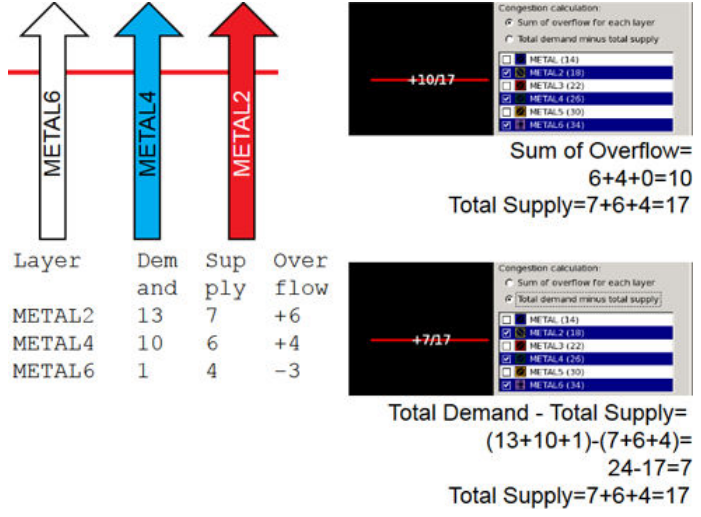
\includegraphics[width=0.92\textwidth]{gui-fig-096.png}
\caption{拥塞示例}
\label{fig:gui-96}
\end{figure}

在本例中，层 METAL2 严重拥塞：布线轨道的需求（demand）为 13，供给（supply）只有 7，溢出为 6。层 METAL4 中等拥塞，溢出为 4。层 METAL6 没有拥塞，下溢（underflow）为 3。本例中其他层不参与拥塞计算。

各层溢出求和是默认计算模式，只考虑每一层的溢出。本例中 METAL2 的溢出为 6，METAL4 的溢出为 4，溢出总和为 $6+4=10$。METAL6 上没有溢出，因此即使选中了该层，也不参与计算。在只含下溢的区域中，工具对每个被选中的层的下溢求和。

Total Demand Minus Total Supply 计算把总需求相加，再减去总供给。本例中总需求为 24，总供给为 17，结果为 $24-17=7$。请注意，在同时含有溢出与下溢的区域中，Total Demand Minus Total Supply 会给出更乐观的拥塞结果。

\subsection{检查拥塞区域中的单元}
\subsubsection*{Examining Cells in Congested Areas}

当拥塞图可见时，可以用拥塞区域对话框在版图视图中定义一个矩形区域，从而查看并选择设计中跨多层的拥塞区域内的单元。对话框列出该区域内拥塞区域中的单元。

可以在单元列表中选择单元，以便在版图视图中查看或高亮它们，也可以设置最小全局布线拥塞（global routing congestion，GRC）违例阈值来过滤单元列表。此外，可以对拥塞区域中的单元做交叉探测（cross-probe），定位到寄存器传输级（register-transfer level，RTL），从而找出可能导致拥塞的 RTL 代码。

要选择并查看拥塞区域中的单元：
\begin{enumerate}
  \item （可选）若只想查看顶层层次上的拥塞区域，选中 “Current design only” 复选框。

  若未选中该复选框（这是默认情况），则显示跨越物理层次的拥塞区域。
  \item 在 Global Route Congestion 面板上单击 “Cells in congested region” 按钮。

  出现拥塞区域对话框。可以把该对话框移到屏幕上某个位置，以便同时使用对话框和版图视图。
  \item 用下列方式之一定义区域的形状与位置：
  \begin{itemize}
    \item 在版图视图中拖动指针，在需要的位置形成矩形；
    \item 或在 “GR Congestion region” 框中输入矩形左上角与右下角的 $x$ 与 $y$ 坐标。
  \end{itemize}
  \item 单击 Apply。

  区域内的单元名称出现在 Cell Name 列表中。列表中只包含高度拥塞区域内的单元。
  \item （可选）要按全局布线拥塞阈值过滤单元，在 “GRC violation threshold” 框中输入一个值。

  只有全局布线阈值大于或等于该值的单元才会出现在对话框中。
  \item 若需要列出设计中另一区域的单元，重复第 2 步到第 4 步。
\end{enumerate}

单元列表树有两种模式：File/Line/Object 与 File/Object。File/Line/Object 模式显示每个文件每一行上的对象。File/Object 模式显示每个文件的对象。

要在版图视图中选择并查看拥塞单元，在单元列表中选择单元名称。版图视图以选择色显示这些选中的单元，选择色默认为白色。

\subsection{交叉探测拥塞区域中的单元}
\subsubsection*{Cross-Probing Cells in Congested Areas}

在拥塞分析期间，对高度拥塞区域中的单元做交叉探测，有助于找出引起拥塞的 RTL 代码。

要快速查看某个单元的 RTL，在 Cells in Congested Region 面板中单击该单元。RTL 代码会在 RTL 浏览器中高亮。

\section{通道拥塞图}
\subsection*{Channel Congestion Map}

通道拥塞图（Channel Congestion map）显示对象之间的通道（channel）中对全局布线需求很高的设计区域。可以为设计中的一小块区域生成通道拥塞图，修改设计后再重新生成 map，以便快速迭代、修复设计中的拥塞区域。要显示全局布线拥塞图，选择 \textbf{View > Map > Global Route Congestion}，或单击 Global Route Congestion 按钮。

要生成通道拥塞图，单击 Reload 按钮。工具显示一个对话框；选择 Whole design area 或 Specified area，以定义要分析通道拥塞的区域。单击 OK 运行命令。完成后，工具显示通道拥塞图。

工具显示通道拥塞图之后，把指针移到版图窗口并放大，以便更细致地查看 map。把指针移到拥塞条上，可在信息提示中查看更多信息。

可以修改 Channel Congestion Map 面板中的设置，以改变拥塞图的显示方式。按下列各项更改拥塞图：
\begin{itemize}
  \item Congestion calculation：选择 Sum of overflow for each layer 或 Total demand minus total supply，以指定计算拥塞的方法。该设置如何影响显示，见「拥塞图计算」。
  \item Bins：更改 Bins 的值，以改变显示 map 所用的唯一分档数目。分档越多，map 被划分成的取值范围就越多。
  \item From: 与 To:：更改这两个值，以改变 map 与直方图中显示的溢出值范围。这些值表示布线单元上布线容量的溢出，数值越大表示拥塞越严重。
  \item Edges：选择要显示拥塞值的全局布线单元的边，即 Horizontal 与 Vertical。
  \item Text：选择此项后，在版图中显示一个代表计算出的密度值的数字。若看不到这些值，必须放大才能查看。
  \item Hierarchical：选择此项后，在层次块内部显示拥塞图。
  \item Layers：选择计算拥塞时要考虑的布线层。
\end{itemize}

修改直方图的更多信息见「配置直方图」。

\section{单元、管脚、块管脚与功耗密度图}
\subsection*{Cell, Pin, Block Pin, and Power Density Maps}

密度图（density map）显示核区域（core area）内、或核内某一矩形区域中，某类对象或某个计算值的高密度（density）区域。IC Compiler II 提供单元密度图（Cell Density Map），用于分析标准单元（standard cell）的密度；提供管脚密度图（Pin Density Map），用于分析给定区域内管脚的密度；并提供功耗密度图（Power Density map），用于分析版图中的功耗密度。块管脚密度图（Block Pin Density map）显示块管脚边上的管脚密度。要显示相应的单元密度图：
\begin{itemize}
  \item 选择 \textbf{View > Map > Cell Density}，或单击 Cell Density 按钮，以显示单元密度图。
  \item 选择 \textbf{View > Map > Pin Density}，或单击 Pin Density 按钮，以显示管脚密度图。
  \item 选择 \textbf{View > Map > Block Pin Density}，或单击 Block Pin Density 按钮，以显示块管脚密度图。
  \item 选择 \textbf{View > Map > Power Density}，或单击 Power Density 按钮，以显示功耗密度图。
\end{itemize}

要生成 map，单击 Reload 按钮。工具显示一个对话框；选择 Whole design area 或 Specified area，以定义要分析的区域。单击 OK 运行命令。完成后，工具显示单元密度图。

工具显示 map 之后，把指针移到版图窗口并放大，以便更细致地查看 map。把指针移到网格点上，可在信息提示中查看更多信息。对于单元密度图、管脚密度图与功耗密度图，Grid size 标签显示当前 map 中水平与垂直网格点的数目。Grid size 的值由每个网格点所含的标准单元高度数目，以及你指定的、用于计算 map 的矩形大小决定。

可以修改 map 面板中的下列设置，以改变显示：
\begin{itemize}
  \item Grid dimension：选择用来为单元密度图、管脚密度图或功耗密度图定义网格的标准单元高度数目。
  \item Solid filled grids：对单元密度图、管脚密度图或功耗密度图，用代表该段版图密度的直方图颜色填充每个网格单元。
  \item Bins：更改 Bins 的值，以改变显示 map 所用的唯一分档数目。分档越多，map 被划分成的取值范围就越多。
  \item From: 与 To:：设置单元密度图、管脚密度图或功耗密度图中显示的密度值范围。
  \item Text：在版图中显示一个数字，表示每个网格点上计算出的密度值。若看不到这些值，必须放大才能查看。
  \item Current design only：只为当前层次级别显示密度图。
\end{itemize}

修改直方图的更多信息见「配置直方图」。

\section{有效电压区域图}
\subsection*{Effective Voltage Areas Map}

有效电压区域图（Effective Voltage Areas map）显示设计的默认电压区域（voltage area）以及其他由用户创建的电压区域。要显示有效电压区域图，选择 \textbf{View > Map > Effective Voltage Areas}，或单击 Effective Voltage Areas 按钮。

工具显示 map 之后，把指针移到某个电压区域上，可在信息提示中查看更多信息。单击该电压区域，即可在 Query 面板中显示有关该电压区域的信息。

可以修改 Effective Voltage Areas map 面板中的设置，以改变 map 的显示方式。按下列各项更改 map 显示：
\begin{itemize}
  \item Show as fractured rectangles：选择此项，把电压区域显示为碎裂矩形（fractured rectangle）。
  \item Hierarchical：选择此项，在层次块内部显示管脚密度图。
\end{itemize}

修改直方图的更多信息见「配置直方图」。

\section{有效站点阵列图}
\subsection*{Effective Site Arrays Map}

有效站点阵列图（Effective Site Arrays map）显示设计中当前已定义的站点阵列（site array）。要显示有效站点阵列图，选择 \textbf{View > Map > Effective Site Arrays}，或单击 Effective Site Arrays 按钮。

工具显示 map 之后，把指针移到站点阵列上，可在信息提示中查看更多信息。单击该站点阵列，即可在 Query 面板中显示有关该站点阵列的信息。

选择 Current design only 选项，则只显示当前层次级别的站点阵列。

修改直方图的更多信息见「配置直方图」。

\section{线利用率图}
\subsection*{Wire Utilization Map}

线利用率图（Wire Utilization map）在版图上显示利用率（utilization）数值。利用率是布线轨道需求除以容量；其中需求是被预布线（preroute）与详细布线图形（detail route shape）占用的轨道数。

要显示线利用率图，从菜单选择 \textbf{View > Map > Wire Utilization}。线利用率图见图~\ref{fig:gui-97}。

\begin{figure}[htbp]
\centering
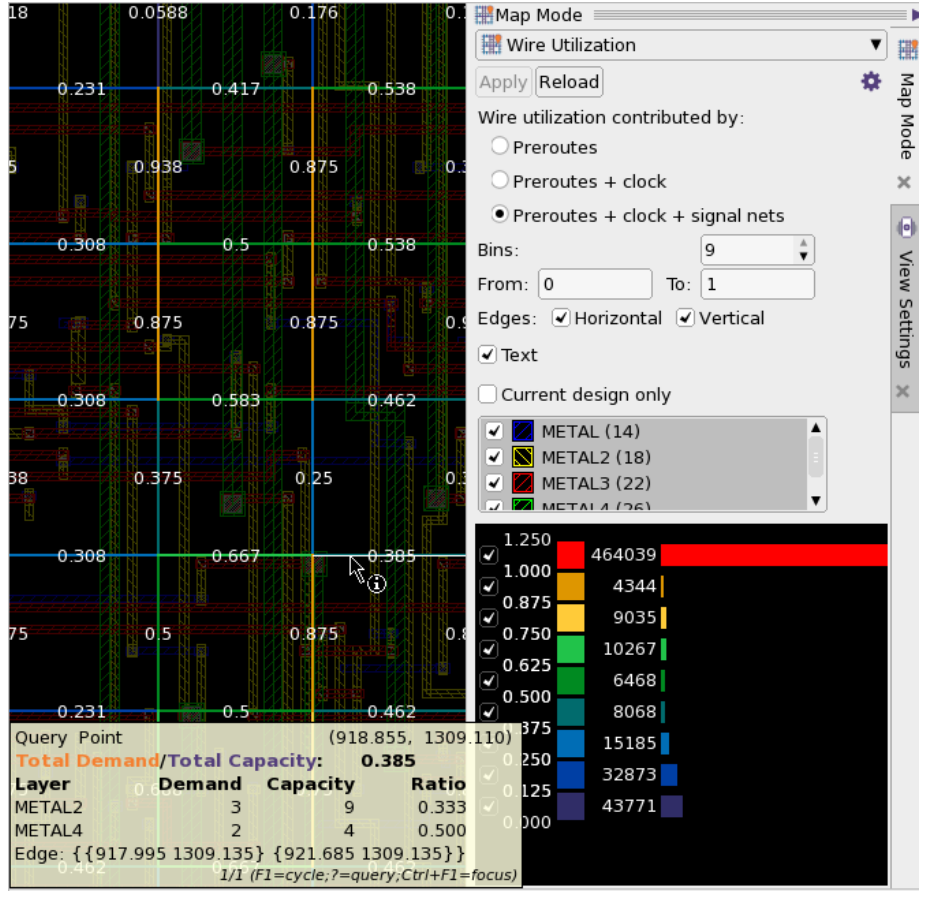
\includegraphics[width=0.92\textwidth]{gui-fig-097.png}
\caption{线利用率图}
\label{fig:gui-97}
\end{figure}

修改 Wire Utilization map 中的设置，以改变 map 的显示方式：
\begin{itemize}
  \item Wire utilization contributed by：选择 Preroutes、Preroutes + clock，或 Preroutes + clock + signal nets。计算需求数时只计入所选的布线类型。
  \item Bins：更改 Bins 的值，以改变显示 map 所用的唯一分档数目。分档越多，map 被划分成的取值范围就越多。
  \item From: 与 To:：更改这两个值，以改变 map 与直方图中显示的溢出值范围。这些值表示布线单元的利用率。
  \item Edges：选择要显示利用率值的边，可以是 Horizontal、Vertical，或两者都选。
  \item Text：在版图中显示一个代表计算出的利用率值的数字。若看不到这些值，必须放大才能查看。
  \item Current design only：把利用率计算限制在当前层次级别。
  \item Layers：选择计算利用率时要考虑的布线层。
\end{itemize}

修改直方图的更多信息见「配置直方图」。

\section{导出与导入 Map 数据}
\subsection*{Exporting and Importing Map Data}

工具支持读取与写出 map 数据。

该功能使你可以：
\begin{itemize}
  \item 以简单的 ASCII 格式导出 map 数据。你可以后处理该 ASCII 文件，或把它作为其他工具的输入。
  \item 把 map 数据导入（或读入）工具，并用 User Map 这一 map mode 生成图或直方图。
\end{itemize}

工具以简单 ASCII 格式读写 map 数据。该格式包含下列部分：元数据（metadata，可选）、表头（header，可选）以及数据。对于可选部分，若未作任何指定，会自动套用默认值。下面是 map 数据文件可能的样子。
% 提取文本在此句之后未保留示例文件正文。

要导出某个特定 map 的 map 数据：
\begin{enumerate}
  \item 在 GUI 中，于版图视图里启用一种 map mode，例如全局布线拥塞图。
  \item 单击 Settings 图标。
  \item 选择 Export as User Map file。
  \item 在 \cmd{gui\_write\_user\_map} 对话框中输入文件名。
  \item 单击 OK。
\end{enumerate}

输出文件以 CSV 格式包含 map 数据。

\begin{noteBox}
输出文件包含整个设计区域的数据，而不是所选区域的数据。工具会忽略未被选中的层。
\end{noteBox}

对于元数据与表头部分中为空的值，工具会自动填入默认值。

{\small
\setlength{\tabcolsep}{3pt}
\begin{longtable}{@{}p{1.05cm}p{0.7cm}p{2.15cm}p{2.55cm}p{1.7cm}p{3.55cm}p{2.15cm}@{}}
\caption{Map 数据 ASCII 文件的元数据默认值}\\
\toprule
类型 & 名称 & 属性 & 值 & 默认值 & 说明 & 示例 \\
\midrule
\endfirsthead
\caption{Map 数据 ASCII 文件的元数据默认值（续）}\\
\toprule
类型 & 名称 & 属性 & 值 & 默认值 & 说明 & 示例 \\
\midrule
\endhead
table & “” & \cmd{app\_name} & string & “” & 用于写出 map 数据的工具 & fc \\
table & “” & \cmd{report\_date} & string & “” & 生成 map 数据的日期与时间 & 2020-Sep-30 09:49:58 \\
table & “” & \cmd{title} & string & \cmd{map\_filename} & Map 标题 & Cell Density \\
table & “” & \cmd{version} & string & “” & 用户 map 版本 & V 1.0 \\
table & “” & \cmd{bins} & int & 10 & Map 的分档计数 & 9 \\
table & “” & \cmd{max\_threshold} & int 或 float & “” & 最大 map 数据 & 1.0 \\
table & “” & \cmd{min\_threshold} & int 或 float & & 最小 map 数据 & 1.0 \\
table & “” & \cmd{color\_scale} & TemperatureScale/RainbowScale/QualitativeScale & TemperatureScale & 三套配色方案，工具按分档数目设置 & TemperatureScale \\
\bottomrule
\end{longtable}
\setlength{\tabcolsep}{6pt}
}

{\small
\setlength{\tabcolsep}{3pt}
\begin{longtable}{@{}p{1.5cm}p{2.6cm}p{1.8cm}p{2.2cm}p{6.2cm}@{}}
\caption{Map 数据 ASCII 文件的表头默认值}\\
\toprule
类型 & 名称 & 属性 & 值 & 说明 \\
\midrule
\endfirsthead
\caption{Map 数据 ASCII 文件的表头默认值（续）}\\
\toprule
类型 & 名称 & 属性 & 值 & 说明 \\
\midrule
\endhead
column & Coordinates type & \cmd{poly\_rect} & &
map 数据的区域，可以是多边形或矩形。矩形的坐标格式为 \cmd{\{llx lly\} \{urx ury\}}（默认）或 \cmd{llx lly urx ury}。例如 \cmd{\{10 10\} \{50 50\}} 或 \cmd{10 10 10 50}。多边形的坐标格式为 \cmd{\{x1 y1\} \{x2 y2\} \ldots\ \{xn yn\}} 或 \cmd{x1 y1 x2 y2 \ldots\ xn yn}，其中 $x_1=x_n$ 且 $y_1=y_n$。例如 \cmd{\{20 20\} \{20 40\} \{30 40\} \{30 30\} \{40 30\} \{40 20\} \{20 20\}} 或 \cmd{20 20 20 40 30 40 30 30 40 30 40 20 20 20}。 \\
column & Value & type & int 或 float & 数据。示例值为 0.835556。 \\
column & Comment & type & string &
数据的文本信息。对于在版图视图中显示对象的 map，注释为对象名。例如 “map\_data: 0.83556”。 \\
column & Comment\_1 & type & string &
可选注释，用来表明数据位于特殊分档中。例如布线拥塞图中的被阻塞区域。 \\
\ldots & \ldots & type & string &
你希望添加的可选注释。其他附加列。 \\
\bottomrule
\end{longtable}
\setlength{\tabcolsep}{6pt}
}

在把 map 数据导入工具之前，可以先预览。

你可能希望在把 map 数据载入工具之前，确认这些数据是准确的。GUI 提供预览对话框，用来预览 map 数据。

要预览 map 数据：
\begin{enumerate}
  \item 确认 map 数据已保存为 CSV 文件。

  关于如何生成 CSV 文件，见「要导出某个特定 map 的 map 数据」。
  \item 使用 \opt{-preview} 选项运行下列命令：
\begin{lstlisting}
icc2_shell> gui_read_user_map -preview -file global_congestion.csv
\end{lstlisting}
  在本例中，\cmd{global\_congestion.csv} 与设计位于同一目录。若文件在其他位置，请给出文件路径。

  出现 (Re)Load User Map Data 对话框，其中的 Column、Base Type、Data Type 与 First Row Values 由 CSV 文件填入。若有错误，对话框会显示这些错误。
  \item （可选）在 CSV 文件中改正错误，并在导入之前预览数据。

  也可以使用 User Map 调色板中的 Reload 按钮来打开预览对话框。
\end{enumerate}

要导入 map 数据：
\begin{enumerate}
  \item 在 GUI 中，于版图视图里启用 User Map 这一 map mode：\textbf{View > Map > User Map}。
  \item 单击 Reload。
  \item 在 (Re)Load User Map Data 对话框中，输入 CSV 文件的名称（含完整路径）。

  载入数据可能需要几分钟。
\end{enumerate}

数据载入完成后，版图视图显示 map 数据。例如：

要把已从文件读入的 map 数据从版图视图中去掉：
\begin{enumerate}
  \item 在 GUI 中，于版图视图里启用 User Map 这一 map mode：\textbf{View > Map > User Map}。
  \item 单击 Remove Current Map。
\end{enumerate}

% 第 6 章续：Visual 模式
\section{Visual 模式概述}
\subsection*{Visual Mode Overview}

Visual mode 在版图视图中用彩色叠加突出设计信息。用 visual mode 可以高亮设计中的不同元素，并把这些元素组织到分档中。如图~\ref{fig:gui-98} 所示，visual mode 支持时钟树（clock tree）、扫描链（scan chain）、相对布局（relative placement）组等对象。要在版图视图中显示或隐藏某种 map mode，选择 \textbf{Highlight > Color By} 并选择一种 visual mode，或单击 Visual Modes 按钮。

Visual mode 支持样式、直方图以及其他配置，说明见「配置 Map 选项」。

\begin{figure}[htbp]
\centering
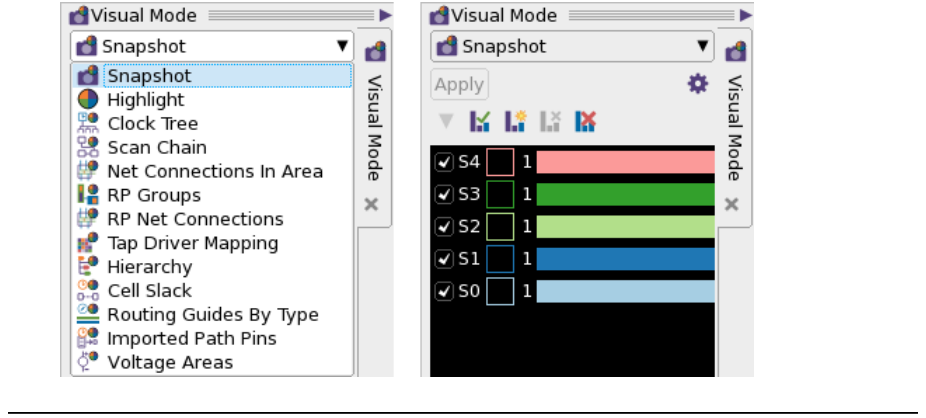
\includegraphics[width=0.92\textwidth]{gui-fig-098.png}
\caption{Visual 模式}
\label{fig:gui-98}
\end{figure}

\section{快照 Visual 模式}
\subsection*{Snapshot Visual Mode}

使用快照 Visual 模式（Snapshot Visual Mode）把一组选中对象收集到一个分档中，并施加高亮颜色。从菜单选择 \textbf{Highlight > Color By > Snapshot}，即可启用快照 Visual 模式。

\begin{figure}[htbp]
\centering
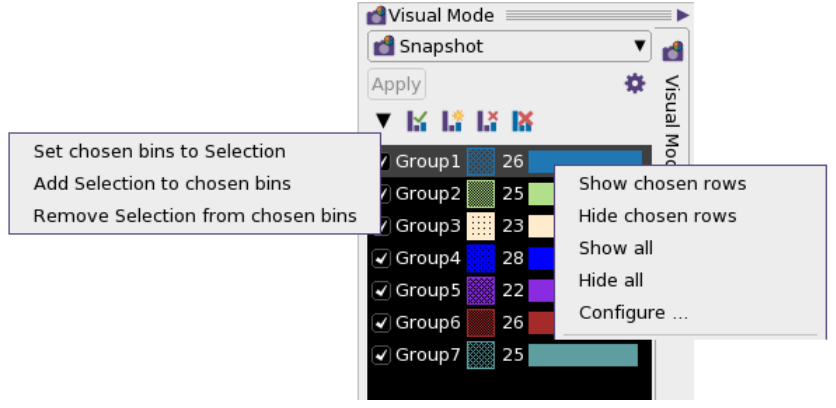
\includegraphics[width=0.92\textwidth]{gui-fig-099.png}
\caption{快照 Visual 模式}
\label{fig:gui-99}
\end{figure}

可以用快照 Visual 模式执行下列操作：
\begin{itemize}
  \item 单击 Copy selection to new bin 按钮，为当前选中的对象着色、创建一个新分档，并把所选对象加入该分档。
  \item 单击 Create a new bin 按钮，创建一个空的新分档。
  \item 单击直方图条以选中该分档，单击面板左侧的向下箭头，并选择 Add selection to chosen bins，即可把选中的对象加入分档。

  使用同一上下文菜单，可以从分档中去掉选中的对象，或用当前选择替换分档中的对象。
  \item 单击某一行以选中它，再单击 Delete chosen row 按钮，即可删除该分档。
  \item 单击 Delete all bins 按钮，从直方图中去掉全部行。
  \item 右键单击直方图行，选择 Set Style，选择新颜色并单击 OK，即可更改高亮颜色。
  \item 右键单击某条直方图条，并在上下文菜单中选择相应项（Move to top、Move up、Move down 或 Move to bottom），即可更改直方图条的顺序或隐藏直方图条。
\end{itemize}

\section{高亮 Visual 模式}
\subsection*{Highlight Visual Mode}

使用高亮 Visual 模式（Highlight Visual Mode）创建直方图，表示按高亮颜色分组后的高亮对象计数。在使用高亮 Visual 模式之前，可以在版图中选中对象并选择 \textbf{Highlight > Selected}，从而高亮这些对象。从菜单选择 \textbf{Highlight > Color By > Highlight}，即可启用高亮 Visual 模式。

\begin{figure}[htbp]
\centering
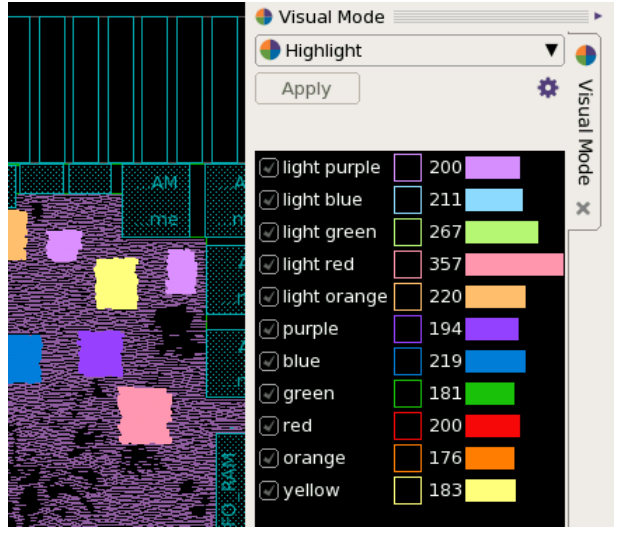
\includegraphics[width=0.92\textwidth]{gui-fig-100.png}
\caption{高亮 Visual 模式}
\label{fig:gui-100}
\end{figure}

在 Highlight Visual Mode 面板中右键单击某条直方图条，可以执行下列操作：
\begin{itemize}
  \item 从上下文菜单选择 Show chosen rows 或 Hide chosen rows，以在版图中显示或隐藏某一直方图行及其对应的高亮颜色。
  \item 从上下文菜单选择 Configure，以配置夸张方案与其他显示选项。
  \item 从上下文菜单选择 Set Style，以更改高亮颜色。
  \item 从上下文菜单选择 Move to top、Move up、Move down 或 Move to bottom，以重排直方图条的顺序。
  \item 选择 Modify Global Selection，并选择用于设置选择、追加选择或从选择中去掉的选项，即可在版图中选中或取消选中已高亮的对象。
\end{itemize}

\section{时钟树 Visual 模式}
\subsection*{Clock Tree Visual Mode}

使用时钟树 Visual 模式（Clock Tree Visual Mode）查看设计中的时钟树，并把相关信息叠加到版图上。

\begin{figure}[htbp]
\centering
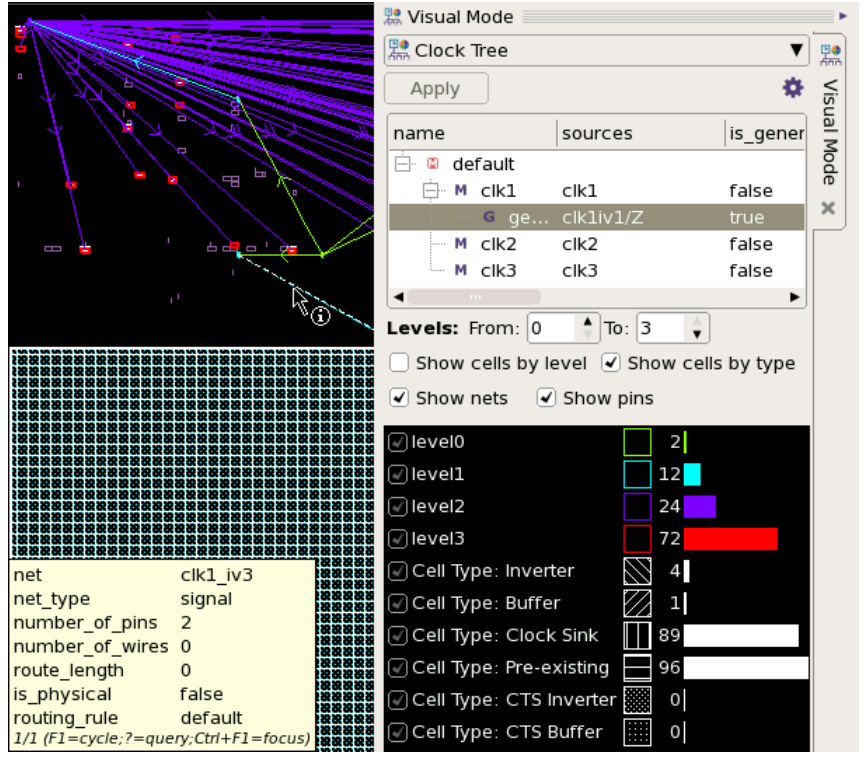
\includegraphics[width=0.92\textwidth]{gui-fig-101.png}
\caption{时钟树 Visual 模式}
\label{fig:gui-101}
\end{figure}

面板显示一张表，列出设计中的时钟源。该表用下列记号显示时钟类型：
\begin{itemize}
  \item M：主时钟（master clock）
  \item G：生成时钟（generated clock）
  \item V：虚拟时钟（virtual clock）
\end{itemize}

面板还显示一张直方图，给出每一级的时钟源、线网与管脚数目，以及每种类型的时钟元件数目。可以用时钟树 Visual 模式执行下列操作：
\begin{itemize}
  \item 单击时钟表中的列标题，按名称、port/pin 或 \cmd{is\_generated} 属性对时钟源排序。
  \item 在面板的 Levels: 部分设置数值，以设定所显示的层次级别范围。
  \item 选择 Show cells by level 选项，按级别显示单元。
  \item 选择 Show cells by type，在版图中加入时钟缓冲器、反相器以及其他单元的单元类型信息。
  \item 选择 Show nets 选项，在版图中显示时钟网飞线（flyline），并把时钟网计数加入直方图。

  选中后，把指针移到时钟网飞线上可显示更多信息。若已做全局布线，工具显示全局布线，而不显示飞线。
  \item 选择 Show pins 选项，显示时钟树中单元的管脚，并把管脚计数加入直方图。
  \item 右键单击直方图行，选择 Set Style，选择新颜色并单击 OK，即可更改高亮颜色。
  \item 在上下文菜单中选择相应项，即可更改直方图条的顺序或隐藏直方图条。
\end{itemize}

\subsection{跟踪时钟树}
\subsubsection*{Tracing Clock Tree}

时钟跟踪器视图提供易于使用的界面，用来跟踪时钟及其相关时钟管脚，一直跟踪到时钟树的漏端管脚。

可以用时钟跟踪器视图：
\begin{itemize}
  \item 优化并调试时钟树综合（clock tree synthesis，CTS）结果；
  \item 查看你可能关心的时钟树漏端。
\end{itemize}

要打开时钟跟踪器视图：
\begin{enumerate}
  \item 选择 \textbf{Window > Clock Tree Analysis Window}。

  把时钟信息载入 CTS 窗口所需的时间，取决于设计是复杂还是简单。复杂设计比简单设计花的时间更长。

  可以过滤时钟与模式，以缩小所显示的信息范围。
  \item 时钟信息载入之后，选择 \textbf{View > Clock Tracer}。

  CTS 窗口按模式组织，显示时钟列表。
\end{enumerate}

要展开时钟树的跟踪，在 CTS 窗口中双击某个时钟或时钟管脚。会出现新的一列，显示该时钟或该时钟管脚所对应的时钟管脚。例如：

单击 Schematic 按钮，可得到时钟层次的图形表示。例如：

使用 Forward 与 Back 按钮，可在时钟层次中导航。

\subsection{检查时钟树重叠}
\subsubsection*{Examining Clock Tree Overlaps}

时钟树重叠分析器视图显示时钟的层次列表或展平列表，以及重叠时钟对的矩阵。重叠矩阵是一个网格，时钟列表中的每个时钟各占一行和一列。

要打开时钟树重叠分析器：
\begin{enumerate}
  \item 选择 \textbf{Window > Clock Tree Analysis Window}。

  把时钟信息载入 CTS 窗口所需的时间，取决于设计是复杂还是简单。复杂设计比简单设计花的时间更长。

  可以过滤时钟与模式，以缩小所显示的信息范围。
  \item 时钟信息载入之后，选择 \textbf{View > Clock Overlap Analyzer}。

  可以过滤时钟与模式，以缩小所显示的信息范围。
\end{enumerate}

在时钟列表中，可展开的层次树表示主时钟与生成时钟之间的时钟层次。可以单击时钟名旁边的展开按钮（加号）来展开该树，从而显示层次中下一级时钟的名称。

重叠矩阵是一个网格，时钟列表中的每个时钟各占一行和一列。矩阵左侧的 Clock 列把列表中的时钟名（包括主时钟与生成时钟）与矩阵中的行、列对应起来。网格中的浅灰色表示这些时钟属于同一时钟域。在时钟列表中选择某个时钟名时，浅蓝色会在矩阵中高亮该时钟所对应的行。背景图案表示哪些时钟处于同一时钟域。

矩阵在网格中显示一个数字，表示该对时钟的重叠点数目。若单击网格中代表一处重叠的方格，工具会在其他视图（例如时钟树原理图或时钟图视图）中用选择色显示该重叠点，选择色默认为白色。

在网格上任意位置右键，可加载上下文相关菜单。菜单中的操作提供更多细节，包括时钟图与时钟属性。从这些细节中可以查看被高亮的重叠点。

\subsection{查看用户定义的偏斜组}
\subsubsection*{Viewing User-Defined Skew Groups}

偏斜组（skew group）使你能够在一个时钟域内平衡不止一组时钟管脚。此外，还可以把集成时钟门控单元（integrated clock-gating cell）的时钟管脚，以及产生时钟的触发器的时钟管脚纳入偏斜组定义，使这些管脚与其他管脚、以及与同一偏斜组定义中的常规漏端一起得到平衡。

使用偏斜组的部分好处：
\begin{itemize}
  \item 可以把与时序关键路径无关的时钟漏端归入一个偏斜组，并放宽该偏斜组的目标偏斜。
  \item 也可以为不同偏斜组分别给出目标早延时（target early delay），从而达到与有用偏斜（useful skew）类似的效果，以改善关键时序路径的裕量（slack）。
\end{itemize}

偏斜组有两种类型：
\begin{itemize}
  \item 默认（Default）：
  \begin{itemize}
    \item 由工具创建；
    \item 每个主时钟定义一个偏斜组，命名为 \cmd{default\_<master\_clock>}；
    \item 这些偏斜组没有与之关联的特定漏端管脚；
    \item 漏端管脚是相关联主时钟的那些管脚。
  \end{itemize}
  \item 用户定义（User-defined）：
  \begin{itemize}
    \item 由用户用 \cmd{create\_clock\_skew\_group} 命令创建；
    \item 每个偏斜组与给定模式相关联；
    \item 每个偏斜组与一份管脚或端口列表相关联。
  \end{itemize}
\end{itemize}

要查看用户定义的时钟偏斜组：
\begin{enumerate}
  \item 选择 \textbf{Window > Clock Tree Analysis Window}。
  \item 选择 \textbf{View > Skew Group Analyzer}。

  时钟树综合窗口同时显示用户定义的时钟偏斜组与默认的时钟偏斜组。

  偏斜组按模式组织。对于用户定义的偏斜组，通往相关联漏端的全部路径都会被高亮。
\end{enumerate}

在时钟树综合窗口中右键单击任意时钟，可以在 Skew Groups 模式与 Clocks 模式之间切换。如下列屏幕截图所示，Skew Groups 模式与 Clocks 模式分别显示与偏斜组、时钟相关的数据。Clocks 模式按时钟显示偏斜组，Skew Groups 模式按偏斜组显示相关时钟。当设计的偏斜组定义很复杂时，这种分类很有帮助。

\begin{figure}[htbp]
\centering
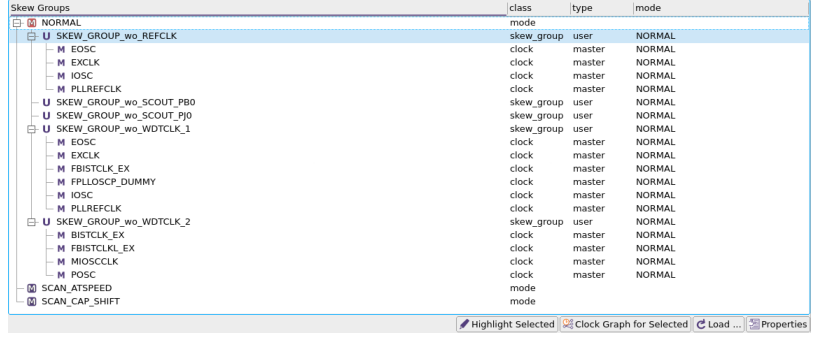
\includegraphics[width=0.92\textwidth]{gui-fig-102.png}
\caption{偏斜组模式}
\label{fig:gui-102}
\end{figure}

\begin{figure}[htbp]
\centering
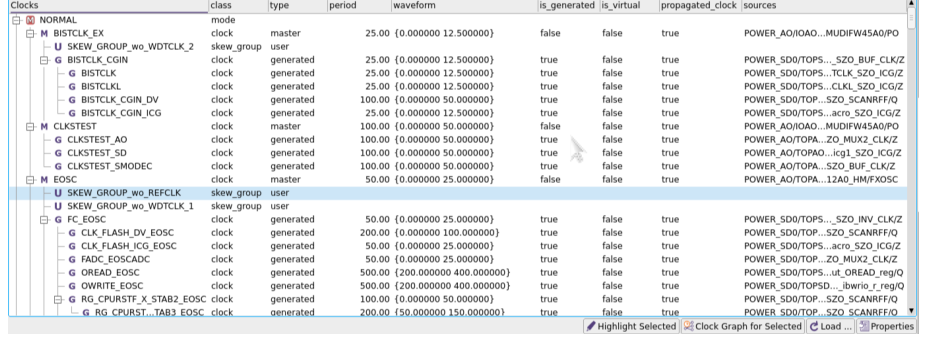
\includegraphics[width=0.92\textwidth]{gui-fig-103.png}
\caption{时钟模式}
\label{fig:gui-103}
\end{figure}

使用 Highlight Selected 菜单，可以在时钟图中高亮所选的时钟或某个偏斜组。例如：

\subsection{查看完整或部分时钟树图}
\subsubsection*{Viewing Full or Partial Clock Tree Graph}

可以用抽象时钟树图（Abstract Clock Tree Graph）查看：
\begin{itemize}
  \item 与该偏斜组的主时钟相关联的全部时钟树；
  \item 只查看与所选用户定义偏斜组相关联的那一部分时钟树。
\end{itemize}

要建立时钟树图：
\begin{enumerate}
  \item 选择 \textbf{Window > Clock Tree Analysis Window}。
  \item 选择 \textbf{View > Skew Group Analyzer}。
  \item 在 CTS 窗口中，右键单击某个偏斜组并选择 Clock Graph。

  打开 Abstract Clock Graph - Levelized 窗口，并显示时钟树。
\end{enumerate}

在该窗口中，也可以查看集成时钟门（integrated clock gate）。

\begin{figure}[htbp]
\centering
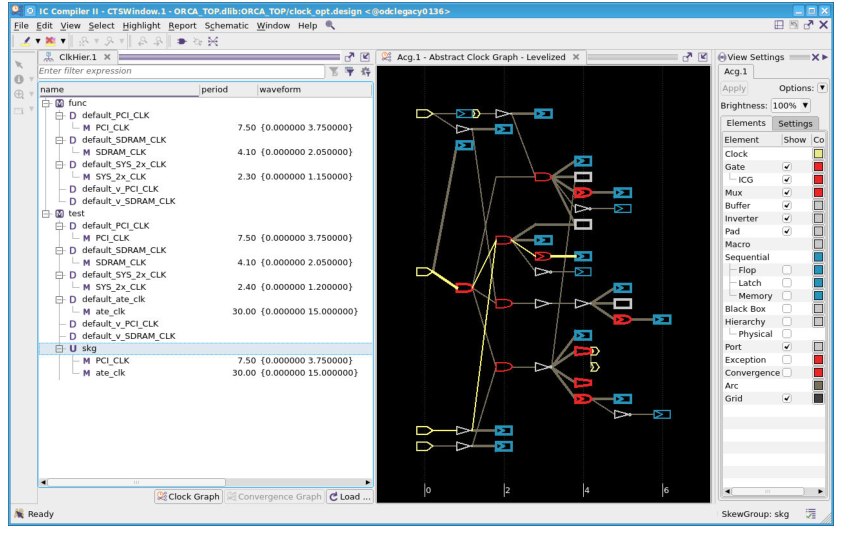
\includegraphics[width=0.92\textwidth]{gui-fig-104.png}
\caption{完整时钟树图}
\label{fig:gui-104}
\end{figure}

\begin{figure}[htbp]
\centering
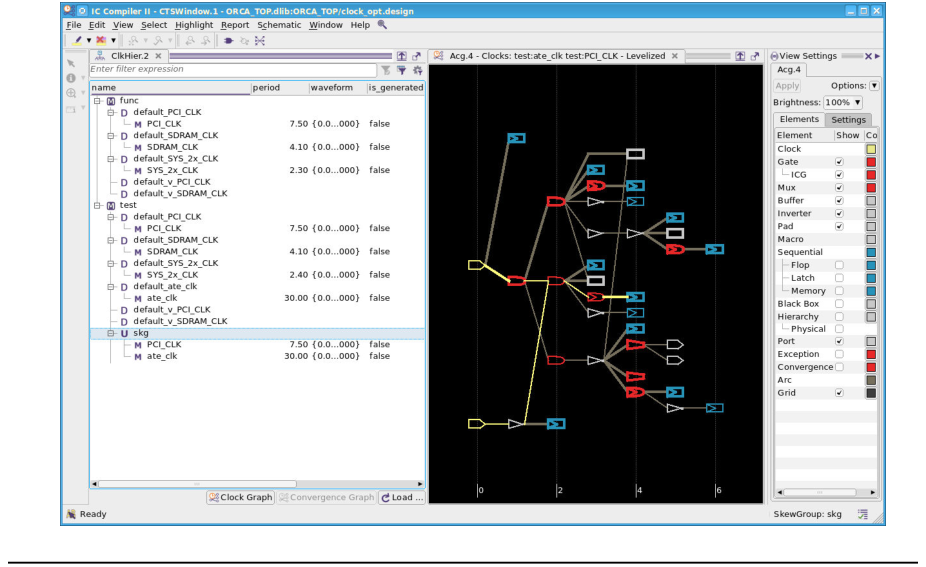
\includegraphics[width=0.92\textwidth]{gui-fig-105.png}
\caption{部分时钟树图}
\label{fig:gui-105}
\end{figure}

\section{扫描链 Visual 模式}
\subsection*{Scan Chain Visual Mode}

使用扫描链 Visual 模式（Scan Chain Visual Mode）显示一条或多条扫描链上扫描输入（scan input）、扫描寄存器（scan register）与扫描输出（scan output）之间的连接。从菜单选择 \textbf{Highlight > Color By > Scan Chain}，即可启用扫描链 Visual 模式。

\begin{figure}[htbp]
\centering
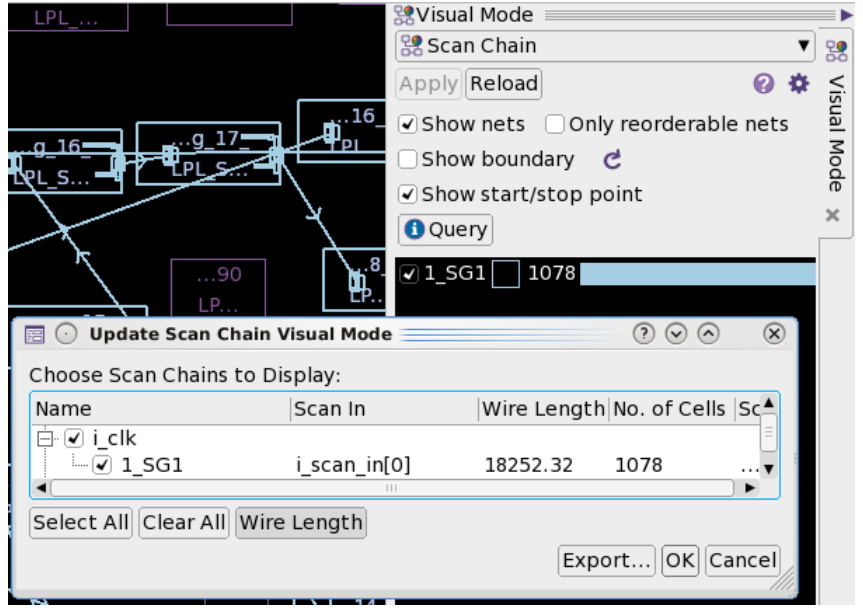
\includegraphics[width=0.92\textwidth]{gui-fig-106.png}
\caption{扫描链 Visual 模式}
\label{fig:gui-106}
\end{figure}

在面板中单击 Reload 之后，可以在 Update Scan Chain Visual Mode 对话框中执行下列操作：
\begin{itemize}
  \item 选中扫描链名称旁边的复选框，并单击 OK 按钮，以在版图窗口中显示所选扫描链。
  \item 单击 Select All 按钮或 Clear All 按钮，对列表中的扫描链执行相应操作。
  \item 单击 Wire Length 按钮，为列表增加一列线长。
  \item 单击某一列并把它拖到新位置，以重排列的顺序。
  \item 把鼠标移到列标题上，单击鼠标右键，并从上下文菜单中选择一项，以配置或排序列表中的列。
\end{itemize}

可以用扫描链 Visual 模式执行下列操作：
\begin{itemize}
  \item 单击 Query 按钮以启动 Query 工具。

  用 Query 工具显示扫描链单元与管脚的更多信息。
  \item 选择 Only reorderable nets 选项，只显示可以重排序的线网。
  \item 选择 Show boundary 选项，显示扫描链的叠加边界。
  \item 选择 Show start/stop point 选项，显示连接到第一条与最后一条扫描链寄存器的端口或管脚连接。
  \item 右键单击直方图行，选择 Set Style，选择新颜色并单击 OK，即可更改高亮颜色。
  \item 在上下文菜单中选择相应项，即可更改直方图条的顺序或隐藏直方图条。
\end{itemize}

\section{区域内线网连接 Visual 模式}
\subsection*{Net Connections in Area Visual Mode}

使用区域内线网连接 Visual 模式（Net Connections in Area Visual Mode）查看与版图中指定区域相交的线网，以帮助在初始布局阶段找出拥塞与布局问题的原因。选择 \textbf{Highlight > Color By > Net Connections in Area}，或单击 Net Connections in Area 按钮，即可启用线网连接 Visual 模式。

\begin{figure}[htbp]
\centering
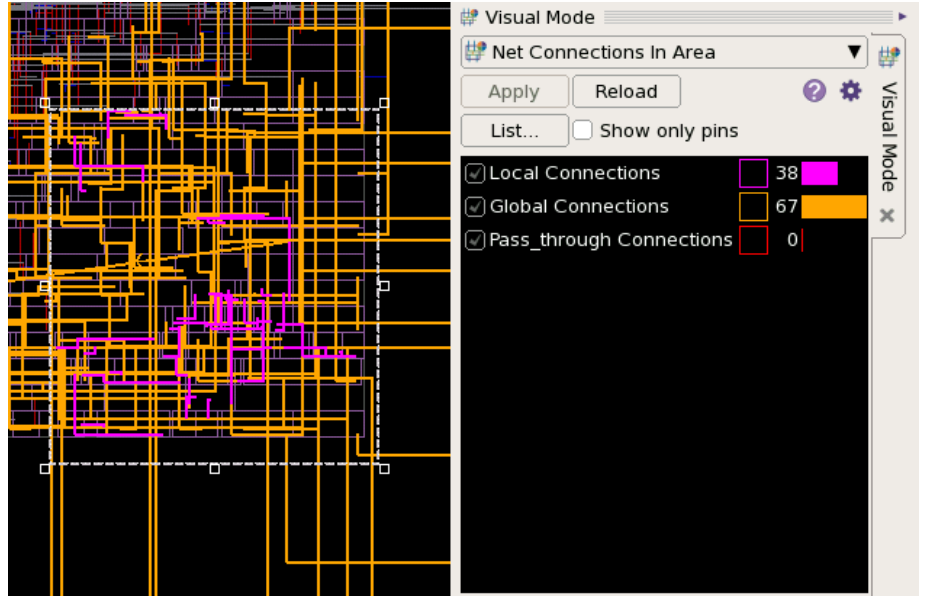
\includegraphics[width=0.92\textwidth]{gui-fig-107.png}
\caption{区域内线网连接}
\label{fig:gui-107}
\end{figure}

工具高亮你所指定区域中的线网，并把它们分成三类：
\begin{itemize}
  \item 局部连接（local connection）：全部管脚与端子都在指定区域之内的线网。
  \item 全局连接（global connection）：至少有一个管脚或端子在指定区域之内，且至少有一个管脚或端子在指定区域之外的线网。
  \item 穿越连接（pass-through connection）：与指定区域相交，但在区域内部没有管脚或端子的线网。
\end{itemize}

要显示指定区域内的线网连接：
\begin{enumerate}
  \item 单击 Reload 按钮，并指定要在其中显示线网的边界框坐标。

  要定义矩形边界，单击区域选择按钮，然后在 Coordinates 框中输入矩形左上角与右下角的 $x$ 与 $y$ 坐标，或在版图视图中拖动指针以形成矩形。
  \item 选择要显示的线网类型（Signal、Clock、Power、Ground、Tie High 或 Tie Low）。
  \item 单击 OK。

  工具显示每一类线网的数目，并按图~\ref{fig:gui-107} 所示在版图窗口中为线网上色。
\end{enumerate}

请注意，图~\ref{fig:gui-107} 显示的是执行全局布线之后的版图。若在执行全局布线之前使用区域内线网连接 Visual 模式，工具显示飞线，而不显示全局布线。

选择 Show only pins，可隐藏工具所高亮的线网，只高亮管脚。修改直方图的更多信息见「配置直方图」。单击 List 按钮，可显示一个对话框，其中包含线网列表，如图~\ref{fig:gui-108} 所示。

\begin{figure}[htbp]
\centering
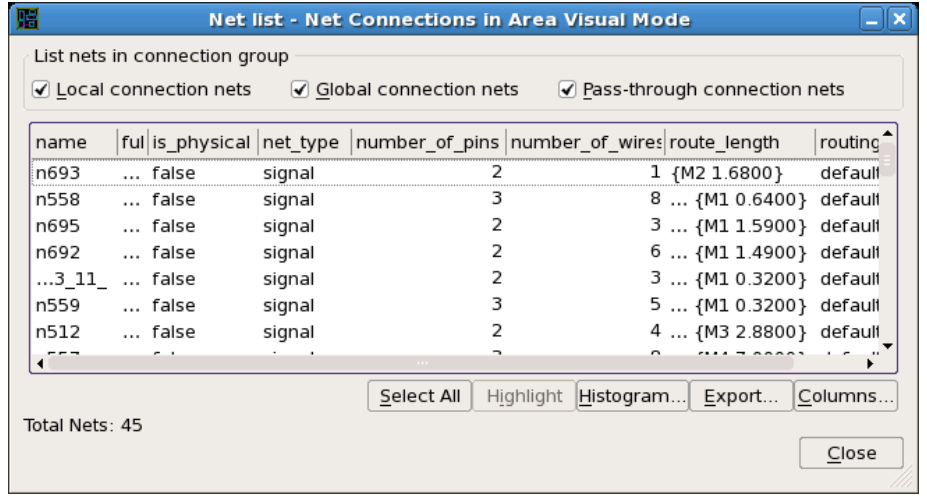
\includegraphics[width=0.92\textwidth]{gui-fig-108.png}
\caption{区域内线网连接列表}
\label{fig:gui-108}
\end{figure}

可以用线网列表对话框执行下列操作：
\begin{itemize}
  \item 单击 Local connection nets、Global connection nets 或 Pass-through connection nets 选项，以切换该线网类型的可见性。
  \item 在线网列表中选择某个线网名，以在版图中高亮该线网。
  \item 单击 Select all 按钮，选择列表中的全部线网。
  \item 单击 Histogram 按钮，配置一个简单直方图，显示区域内的管脚数目或线网数目；在对话框中单击 OK，即可生成直方图，并把它显示在版图窗口的直方图面板中。
  \item 单击 Export 按钮，把表的内容写成逗号分隔值格式的文件。
  \item 单击 Columns 按钮，配置要显示哪些数据列。
\end{itemize}

\section{相对布局（RP）组 Visual 模式}
\subsection*{Relative Placement (RP) Groups Visual Mode}

使用 RP 组 Visual 模式高亮相对布局组。从菜单选择 \textbf{Highlight > Color By > RP Groups}，即可启用 RP 组 Visual 模式。

\begin{figure}[htbp]
\centering
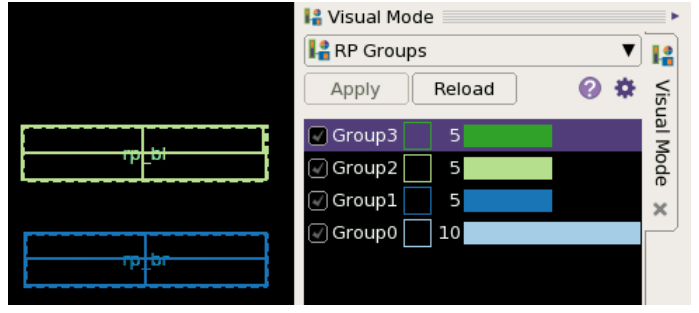
\includegraphics[width=0.92\textwidth]{gui-fig-109.png}
\caption{RP 组 Visual 模式}
\label{fig:gui-109}
\end{figure}

可以用 RP 组 Visual 模式执行下列操作：
\begin{itemize}
  \item 单击 Reload 并单击 OK，高亮设计中的相对布局组。
  \item 选择 Color by RP group，按组名高亮相对布局组。
  \item 选择 Color by RP hierarchical level，按相对布局组在层次中的位置高亮它们。
  \item 选择 Color cell only 选项，只高亮相对布局组中的单元。
  \item 在 Maximum number of colors 框中输入新值，以增加或减少被高亮的组数。可以输入 5 到 20 之间的整数。
  \item 右键单击某条直方图条，选择 Modify Global Selection，并选择用于设置选择、追加选择或从选择中去掉的选项，即可在版图中选中或取消选中相对布局组。
  \item 在上下文菜单中选择相应项，即可更改直方图条的顺序或隐藏直方图条。
\end{itemize}

\section{相对布局（RP）线网连接 Visual 模式}
\subsection*{Relative Placement (RP) Net Connection Visual Mode}

使用 RP 线网连接 Visual 模式高亮连接相对布局组的线网。从菜单选择 \textbf{Highlight > Color By > RP Net Connections}，即可启用 RP Visual 模式。

\begin{figure}[htbp]
\centering
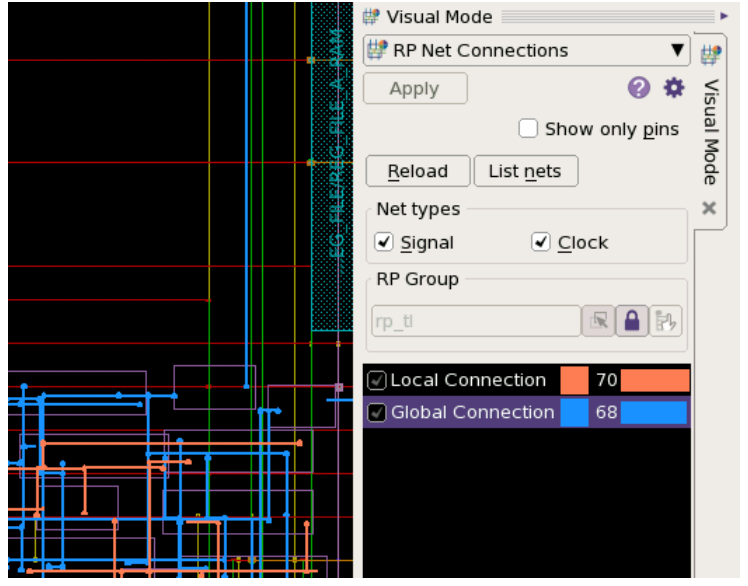
\includegraphics[width=0.92\textwidth]{gui-fig-110.png}
\caption{RP 线网连接 Visual 模式}
\label{fig:gui-110}
\end{figure}

要显示 RP 线网连接：
\begin{enumerate}
  \item 在 RP Group 框中指定一个或多个 RP 组名，或单击 Browse for RP group 按钮并选择一个或多个组。
  \item 选择 Signal 选项以显示信号网，选择 Clock 选项以显示时钟网，或同时选择两项以显示两类线网。
  \item 单击 Reload 按钮，在版图中显示指定 RP 组的 Net Connections。
  \item （可选）单击 List nets 按钮打开对话框，显示指定 RP 组的局部连接与全局连接，如图~\ref{fig:gui-111} 所示。

  用该对话框选择、高亮或导出线网，做法见「区域内线网连接 Visual 模式」。
\end{enumerate}

\begin{figure}[htbp]
\centering
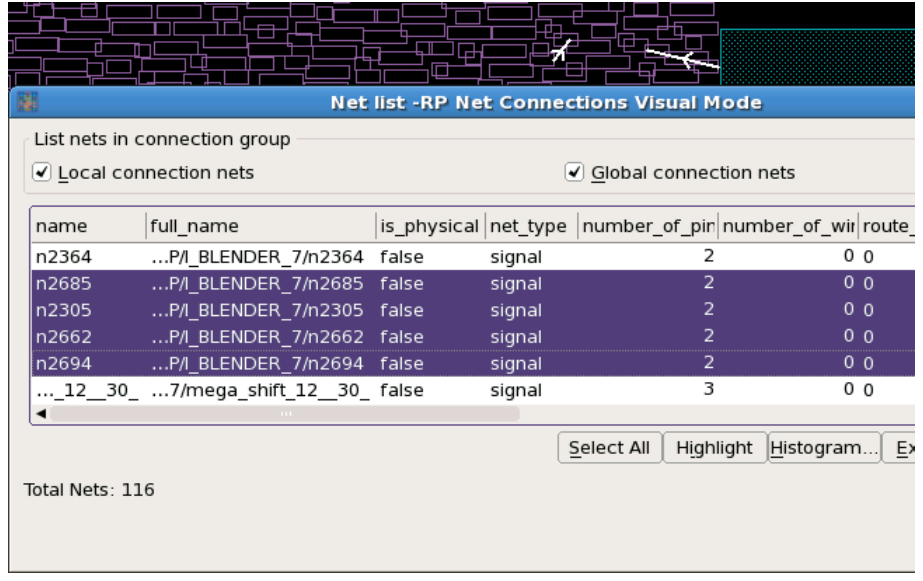
\includegraphics[width=0.92\textwidth]{gui-fig-111.png}
\caption{RP 线网连接列表}
\label{fig:gui-111}
\end{figure}

可以用 RP 线网连接 Visual 模式执行下列操作：
\begin{itemize}
  \item 选择 Show only pins 选项，只高亮连接到 RP 线网连接的管脚。
  \item 选中或取消 Local Connection 或 Global Connection 旁边的复选框，以显示或隐藏 RP 线网连接的飞线。

  局部连接是只连接到同一相对布局组内单元的线网。全局连接至少把相对布局组中的一个单元连接到相对布局组之外的至少一个单元。
  \item 右键单击某条直方图条，选择 Modify Global Selection，并选择用于设置选择、追加选择或从选择中去掉的选项，即可在版图中选中或取消选中相对布局线网连接。
  \item 在上下文菜单中选择相应项，即可更改直方图条的顺序或隐藏直方图条。
\end{itemize}

\section{层次 Visual 模式}
\subsection*{Hierarchy Visual Mode}

使用层次 Visual 模式（Hierarchy Visual Mode）高亮并选择设计中的不同层次级别，或特定的层次单元。从菜单选择 \textbf{Highlight > Color By > Hierarchy}，即可启用层次 Visual 模式。

\begin{figure}[htbp]
\centering
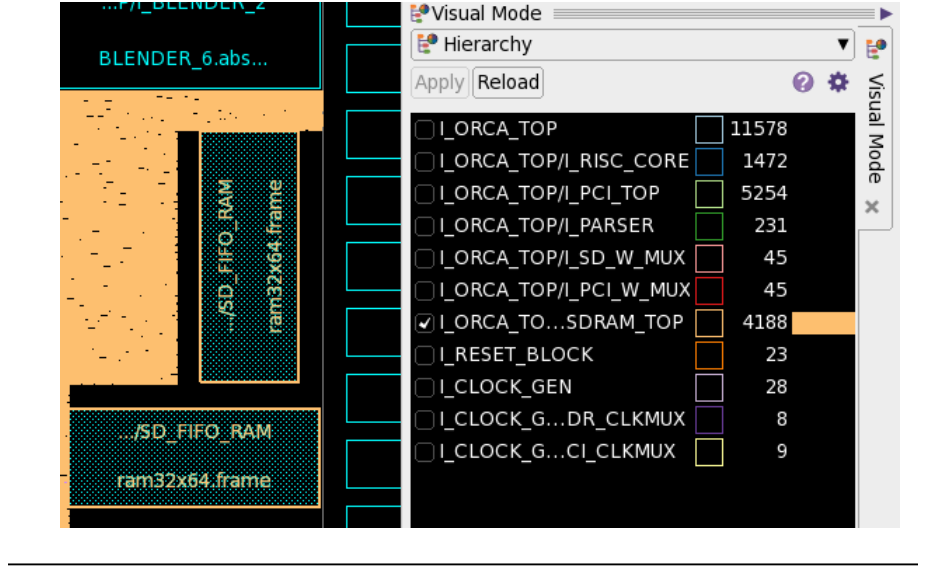
\includegraphics[width=0.92\textwidth]{gui-fig-112.png}
\caption{层次 Visual 模式}
\label{fig:gui-112}
\end{figure}

\section{单元裕量 Visual 模式}
\subsection*{Cell Slack Visual Mode}

使用单元裕量 Visual 模式（Cell Slack Visual Mode）查看设计中的建立（setup）与保持（hold）时序裕量，并把这些信息叠加到版图上。从菜单选择 \textbf{Highlight > Color By > Cell Slack}，即可打开该面板。

\begin{figure}[htbp]
\centering
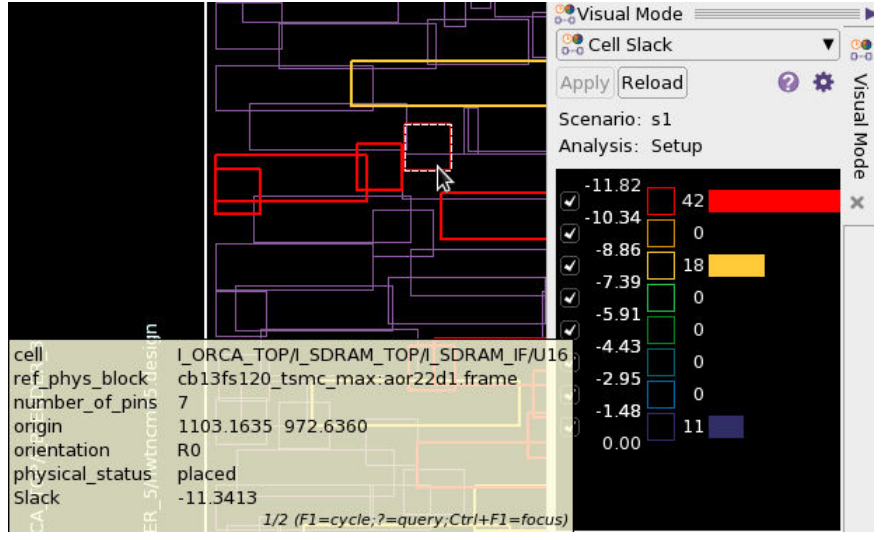
\includegraphics[width=0.92\textwidth]{gui-fig-113.png}
\caption{单元裕量 Visual 模式}
\label{fig:gui-113}
\end{figure}

单击 Reload 按钮，并在对话框中选择选项，即可开始单元裕量分析。设置选项之后，单击 OK 以生成数据。Cell Slack 对话框支持下列操作：
\begin{itemize}
  \item 从框中选择场景（scenario）名称，以指定要分析的场景。
  \item 选择 Setup 或 Hold 选项，以显示建立时间裕量或保持时间裕量信息。
  \item 选择 Number of bins，并选择一个大于零的整数，以指定划分裕量结果所用的分档数目。

  也可以选择 Value range per bin，并指定最小与最大单元裕量值，从而指定每个分档的取值范围。单击 Lower bound strict 或 Upper bound strict 选项，可把指定范围之外的裕量值从直方图中去掉。
  \item 在 Cells 框中输入单元名列表，或选中单元并单击 populate from selection 按钮，以分析特定单元。
  \item 选择 Temperature 或 Gradient 选项，以更改直方图所用的调色板。
\end{itemize}

\section{导入路径管脚 Visual 模式}
\subsection*{Imported Path Pins Visual Mode}

使用导入路径管脚 Visual 模式（Imported Path Pins Visual Mode）在版图中高亮时序路径。从菜单选择 \textbf{Highlight > Color By > Imported Path Pins}，即可启用导入路径管脚 Visual 模式。

\begin{figure}[htbp]
\centering
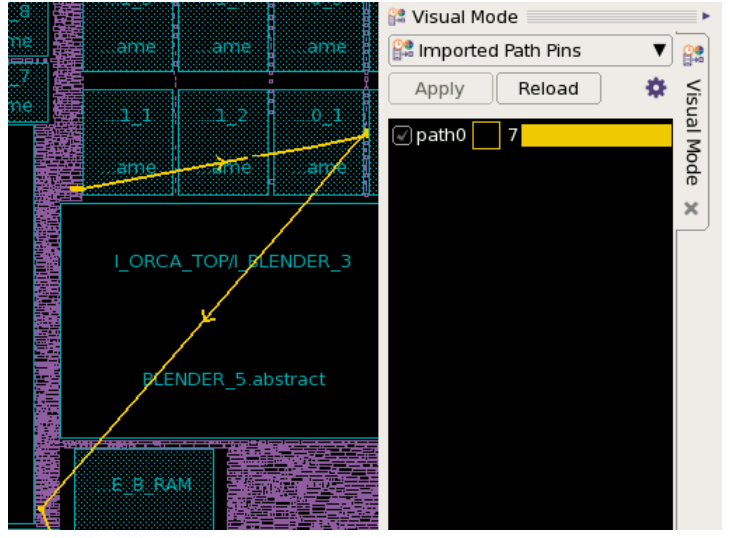
\includegraphics[width=0.92\textwidth]{gui-fig-114.png}
\caption{导入路径管脚 Visual 模式}
\label{fig:gui-114}
\end{figure}

要导入一条时序路径并在版图中高亮该路径：
\begin{enumerate}
  \item 选择 \textbf{Highlight > Color By > Imported Path Pins}，打开导入路径管脚 Visual 模式。
  \item 用 \cmd{update\_timing} 命令更新设计的时序。
\begin{lstlisting}
icc2_shell> update_timing -full
\end{lstlisting}
  \item 用 \cmd{report\_timing} 命令报告一条路径的时序，并把结果保存到文件。
\begin{lstlisting}
icc2_shell> report_timing \
   -from I_RESET_BLOCK/sdram_rst_n_buf_reg \
   -to I_ORCA_TOP/I_SDRAM_TOP/I_SDRAM_IF/DQ_out_1_reg_6_ -nosplit \
   -physical > timing.rpt
\end{lstlisting}
  \item 单击 Reload 按钮。
  \item 选择 Import Path Pins from Timing Report，并单击文件选择按钮。
  \item 选择你在第 3 步写出的 \cmd{timing.rpt} 文件，并单击 OK。

  Imported Path Pins Visual Mode 面板为该路径显示一条直方图条，并给出路径中的管脚数目。工具还会在版图视图中显示该路径的飞线。
  \item 重复第 3 步到第 6 步，以导入并显示更多路径。选择 Clear all buckets before importing new path pins 选项，可在导入新路径之前删除直方图。
\end{enumerate}

除了按第 5 步与第 6 步选择 Import Path Pins 选项并导入文件之外，还可以选择 Import from timing report text，并把时序报告的内容粘贴到文本框中，如图~\ref{fig:gui-115} 所示。

\begin{figure}[htbp]
\centering
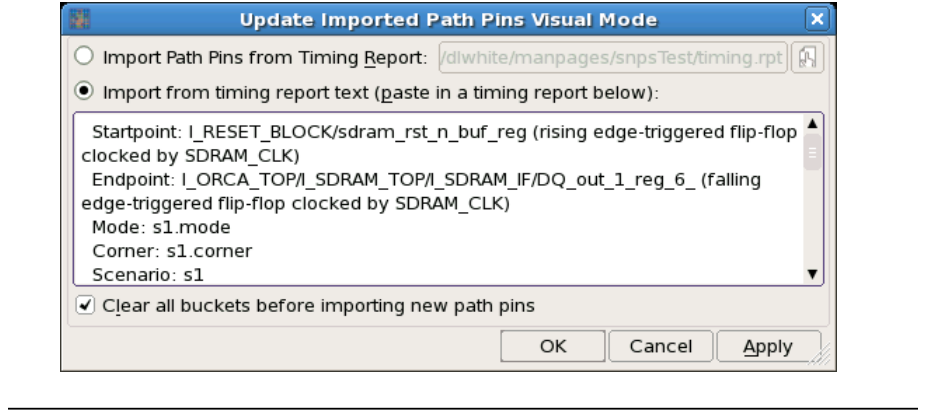
\includegraphics[width=0.92\textwidth]{gui-fig-115.png}
\caption{从时序报告文本导入}
\label{fig:gui-115}
\end{figure}

\section{电压区域 Visual 模式}
\subsection*{Voltage Areas Visual Mode}

使用电压区域 Visual 模式（Voltage Areas Visual Mode）高亮并选择设计中的电源域（power domain）、电平移位器（level shifter）、隔离单元（isolation cell），以及其他与电源域相关的单元。从菜单选择 \textbf{Highlight > Color By > Voltage Areas}，即可启用电压区域 Visual 模式。

\begin{figure}[htbp]
\centering
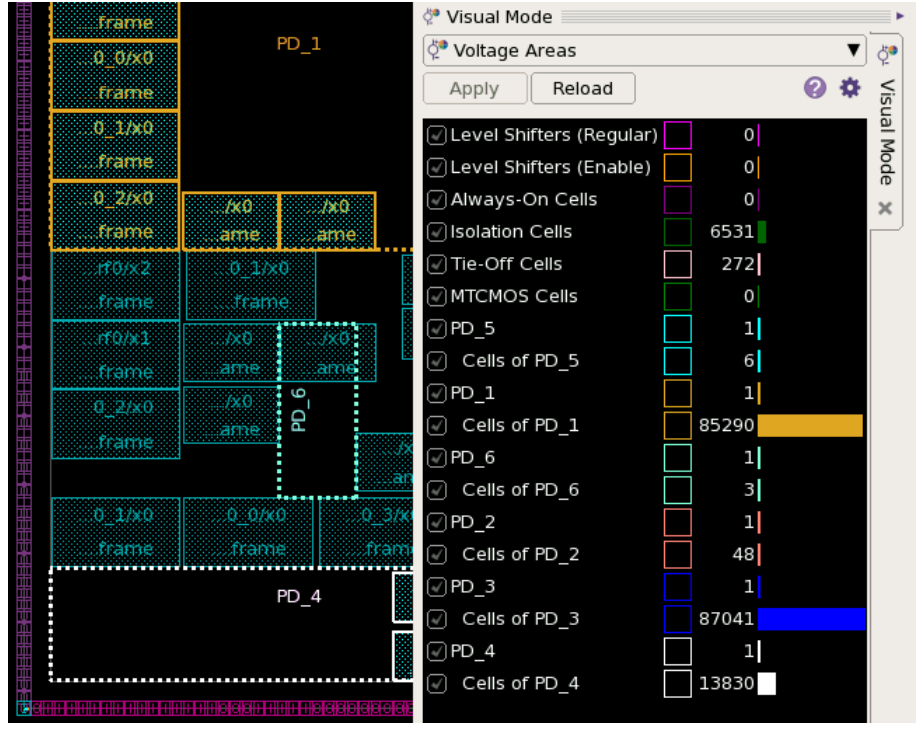
\includegraphics[width=0.92\textwidth]{gui-fig-116.png}
\caption{电压区域 Visual 模式}
\label{fig:gui-116}
\end{figure}

单击 Reload 按钮，以填充 Voltage Areas Visual Mode 面板。右键单击某条直方图条，并从上下文菜单中选择一项，即可更改颜色、在列表中上移或下移该条、在版图中选择相关对象、显示或隐藏该直方图条，以及执行其他操作。


% 第 7 章 Viewing Schematics
\bichapter{查看原理图}{Viewing Schematics}
\label{chap:gui-sch}

IC Compiler II 支持设计原理图，用来查看设计中的逻辑元件（块与门）。原理图以图形显示层次单元。可以在设计层次中向上或向下，查看每一层设计的原理图。

本章包括以下主题：
\begin{itemize}
  \item 原理图视图
  \item 原理图中的 WordView
  \item 在原理图上标注属性
  \item 在原理图上添加管脚标记
\end{itemize}

\section{原理图视图}
\subsection*{Schematic View}

查看原理图：
\begin{itemize}
  \item 在主菜单或 Hierarchy Browser 中选择 \textbf{View > Schematic View}；
  \item 或单击工具栏上的原理图按钮。
\end{itemize}

原理图视图用于直观分析时序与逻辑，供后续优化使用。例如可以：
\begin{itemize}
  \item 查看设计或子设计中逻辑元件（块与门）的图形；
  \item 聚焦关键路径，检查时序问题。
\end{itemize}

要定制原理图视图，使用工具右侧选项卡中的 View Settings 面板。视图属性的保存方式见第~\ref{chap:gui-start}~章。

\begin{seeAlsoBox}
设置并保存视图属性，见第~\ref{chap:gui-start}~章。
\end{seeAlsoBox}

\section{原理图中的 WordView}
\subsection*{WordView in the Schematic View}

WordView 用宽组合逻辑门建立模型，便于在原理图中表示。对尚未映射的逻辑，WordView 让原理图更干净：工具用一个宽逻辑门代替级联门，并把总线实例显示为折叠形式。做面积估算时，WordView 能更准确地反映 RTL 中的原始逻辑。

WordView 使用 WVGTECH 库，而不是 GTECH 库。工具要推断这些门，必须能用到 WVGTECH 库。

在原理图视图中，GUI 用 WordView 门显示：
\begin{itemize}
  \item 总线实例（bused instance）
  \item 宽门（wide gate）
  \item 运算符（operator）
  \item 映射到多位单元的总线寄存器
\end{itemize}

图~\ref{fig:gui-117} 是折叠后的总线实例，这里是一个四输入的 WVGTECH\_AND。

\begin{figure}[htbp]
\centering
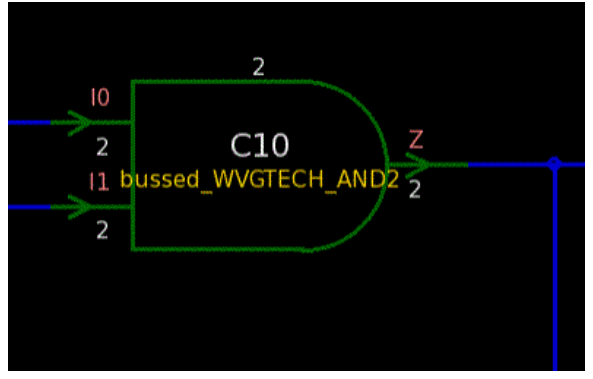
\includegraphics[width=0.72\textwidth]{gui-fig-117.png}
\caption{总线实例的折叠视图}
\label{fig:gui-117}
\end{figure}

选中 WVGTECH 门，打开上下文菜单并选择 \textbf{Expand > Selected Objects}，即可展开。默认情况下，总线实例以虚线边框显示，见图~\ref{fig:gui-118}。总线网用一条粗蓝线表示，总线反相器使用同一逻辑符号加一条粗绿线。对总线对象，可用原理图上下文菜单中的 Expand 或 Collapse 在标量表示与总线表示之间切换。

\begin{figure}[htbp]
\centering
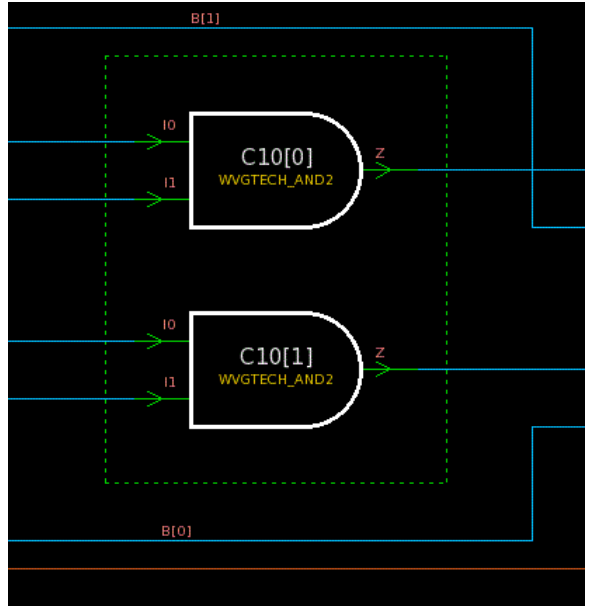
\includegraphics[width=0.72\textwidth]{gui-fig-118.png}
\caption{总线实例的展开视图}
\label{fig:gui-118}
\end{figure}

图~\ref{fig:gui-119} 是 WordView 宽门的例子。该 XOR 有 16 个输入管脚，名为 WVGTECH\_XOR16。

\begin{figure}[htbp]
\centering
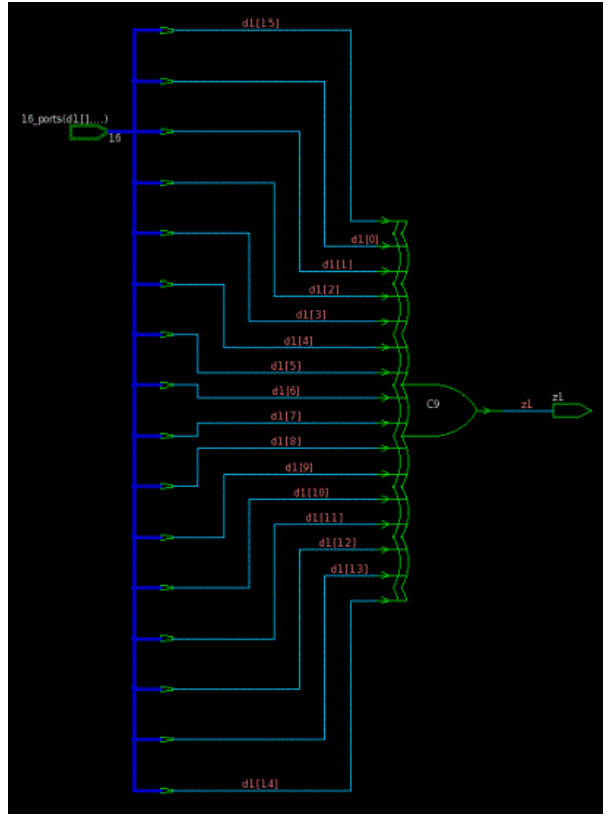
\includegraphics[width=0.55\textwidth]{gui-fig-119.png}
\caption{宽门示例}
\label{fig:gui-119}
\end{figure}

运算符在 GUI 中画成基本符号，见图~\ref{fig:gui-120}。此例表示加法运算符。

\begin{figure}[htbp]
\centering
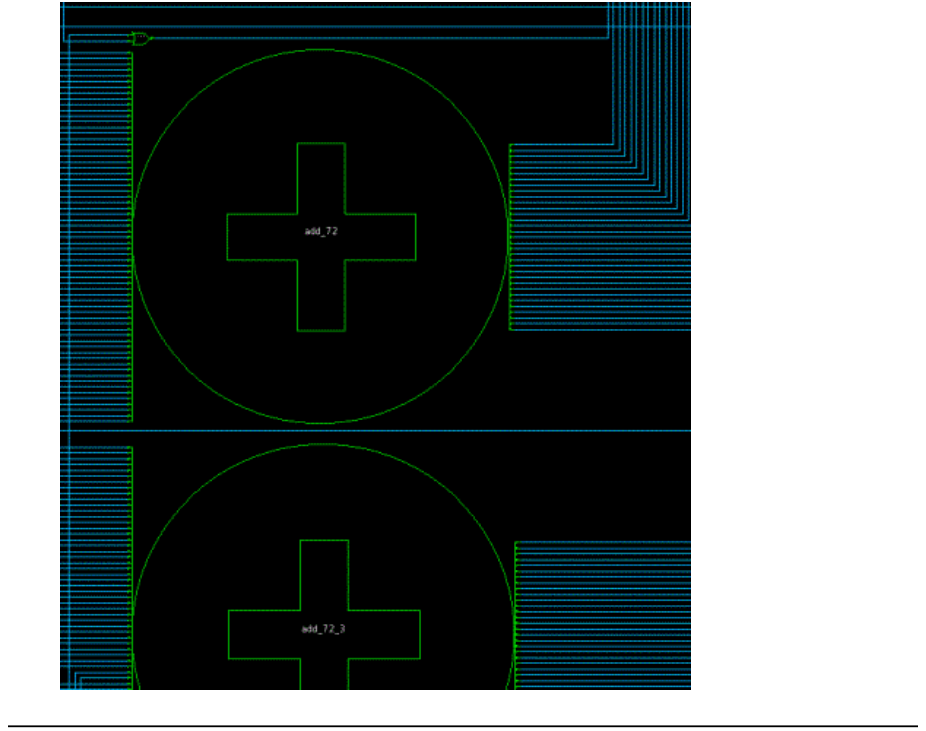
\includegraphics[width=0.45\textwidth]{gui-fig-120.png}
\caption{运算符示例}
\label{fig:gui-120}
\end{figure}

\section{在原理图上标注属性}
\subsection*{Annotating Attributes on the Schematic View}

调试时，可以在原理图的单元、管脚和端口上标注属性。在 View Settings 面板 Settings 页的 Annotation Attributes 区选择要标注的属性，见图~\ref{fig:gui-121}。每个对象只能标注一个属性。

\begin{figure}[htbp]
\centering
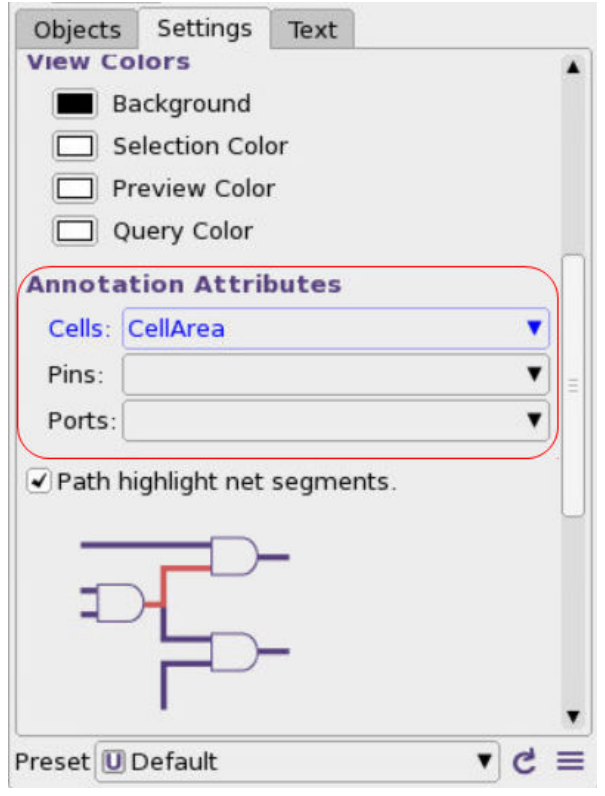
\includegraphics[width=0.8\textwidth]{gui-fig-121.png}
\caption{Settings 页中的 Annotation Attributes}
\label{fig:gui-121}
\end{figure}

图~\ref{fig:gui-122} 中，属性标注为白色：单元上标注 area，管脚上标注 port\_type。

\begin{figure}[htbp]
\centering
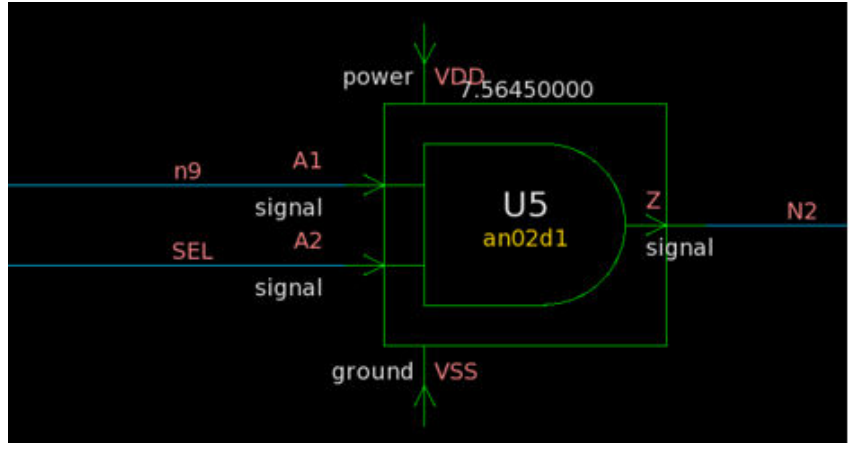
\includegraphics[width=0.8\textwidth]{gui-fig-122.png}
\caption{单元与管脚上的属性标注}
\label{fig:gui-122}
\end{figure}

可以用它调试时序违例，例如在路径管脚上标注 \cmd{late\_rise\_transtion}；也可以分析功耗，例如在路径管脚上标注 \cmd{switching\_activity} 或 \cmd{toggle\_rate}。

\section{在原理图上添加管脚标记}
\subsection*{Adding Pin Markers to the Schematic View}

可以在原理图管脚上加标记，以突出内容。标记可选：
\begin{itemize}
  \item 形状：菱形（diamond）或圆点（dot）；
  \item 颜色：黄、橙或红。
\end{itemize}

右键单击管脚，选择 \textbf{Pin Markers > Set > }\textit{marker\_type}。\textit{marker\_type} 为 Yellow Diamond、Orange Diamond、Red Diamond、Yellow Dot、Orange Dot 或 Red Dot 之一。界面见图~\ref{fig:gui-123}。

\begin{figure}[htbp]
\centering
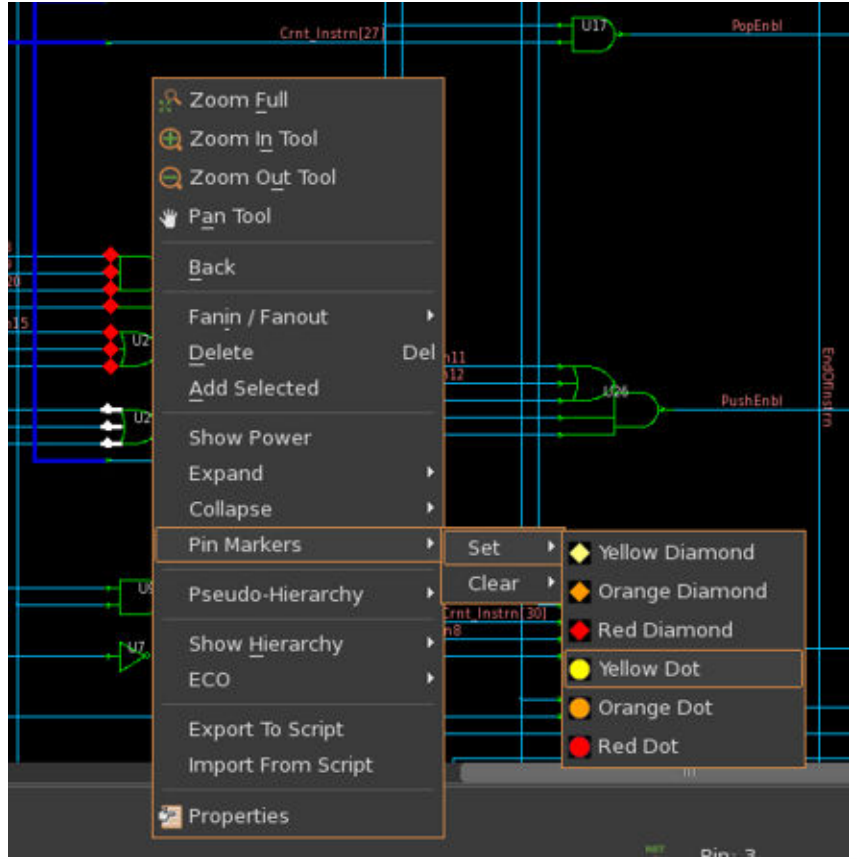
\includegraphics[width=0.7\textwidth]{gui-fig-123.png}
\caption{添加管脚标记}
\label{fig:gui-123}
\end{figure}

% 第 8 章 Timing Analysis Using the GUI
\bichapter{用 GUI 做时序分析}{Timing Analysis Using the GUI}
\label{chap:gui-timing}

用 GUI 查看时序分析结果，并对有问题的时序路径做交互查询。

本章包括以下主题：
\begin{itemize}
  \item 打开时序分析窗口
  \item 显示时序分析端点摘要
  \item 创建路径集合
  \item 分析时序路径集合
  \item 分析逻辑级数
\end{itemize}

\section{打开时序分析窗口}
\subsection*{Opening the Timing Analysis Window}

设计编译完成后，可用 GUI 查看时序分析结果。

\begin{enumerate}
  \item 用 Timing Analysis 窗口取得端点摘要。在主菜单选择 \textbf{Window > Timing Analysis Window}。
  \item 按端点摘要创建路径集合。
  \item 分析所选路径集合的时序裕量（slack）。
\end{enumerate}

\begin{seeAlsoBox}
显示端点摘要、创建路径集合，以及分析逻辑级数，见本章后续各节。
\end{seeAlsoBox}

\section{显示时序分析端点摘要}
\subsection*{Displaying the Timing Analysis Endpoint Summary}

Timing Analysis 窗口显示当前设计的时序摘要，应与 \cmd{report\_qor -summary} 的结果一致。

用这些信息做分析之前，先确认时序是最新的。绿色对勾表示时序已更新；否则显示红色标记。要更新时序，单击 Update，见图~\ref{fig:gui-124}。

\begin{figure}[htbp]
\centering
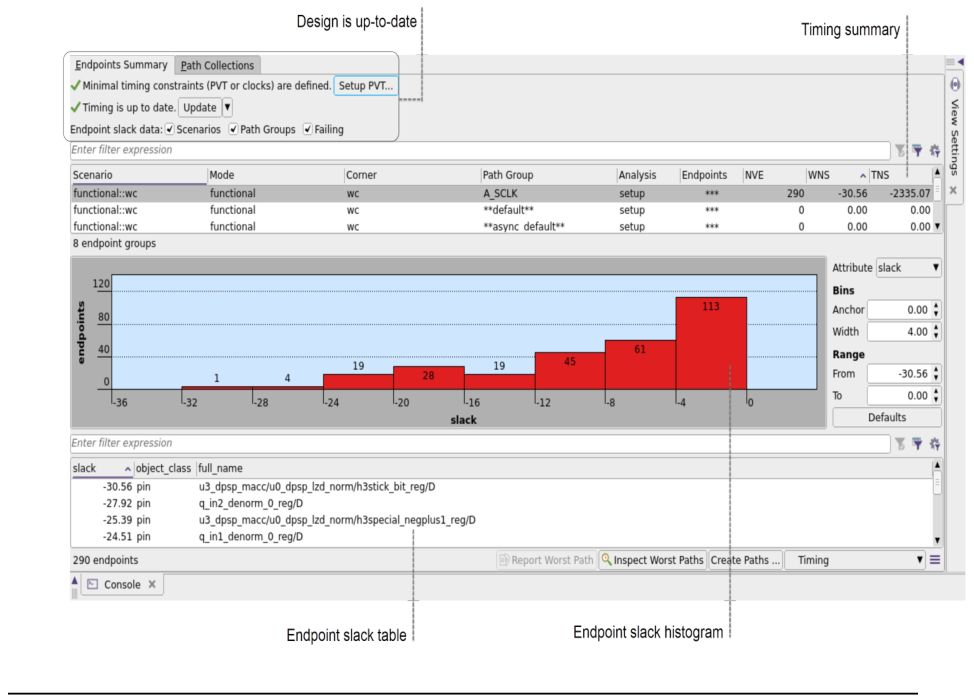
\includegraphics[width=0.92\textwidth]{gui-fig-124.png}
\caption{时序分析摘要窗口}
\label{fig:gui-124}
\end{figure}

\section{创建路径集合}
\subsection*{Creating Path Collections}

在 Timing Analysis 窗口的 Endpoints Summary 选项卡中，可以创建路径集合来选择要分析的路径。在窗口底部的 Endpoint Slack Table 中选择端点，再选择 Create Paths，见图~\ref{fig:gui-125}。

\begin{figure}[htbp]
\centering
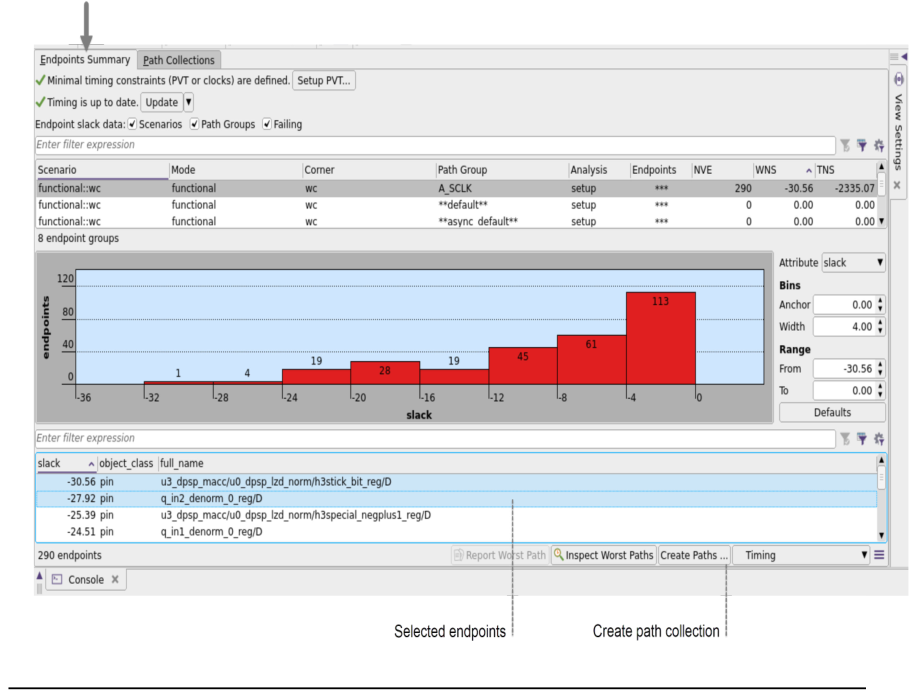
\includegraphics[width=0.92\textwidth]{gui-fig-125.png}
\caption{创建路径集合}
\label{fig:gui-125}
\end{figure}

\subsection{获取时序路径}
\subsubsection*{Getting Timing Paths}

单击 Create Paths 后出现 Get Timing Paths 对话框，见图~\ref{fig:gui-126}。

\begin{figure}[htbp]
\centering
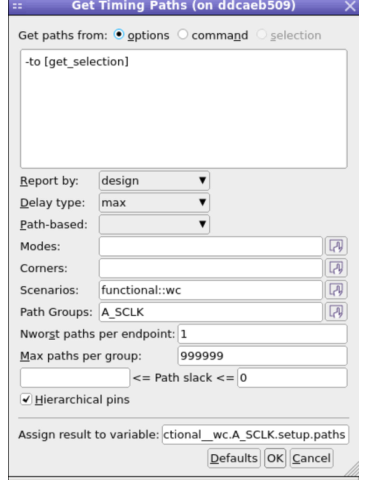
\includegraphics[width=0.8\textwidth]{gui-fig-126.png}
\caption{Get Timing Paths 对话框}
\label{fig:gui-126}
\end{figure}

在该对话框中填写选项，按设计、组、场景（scenario）、模式（mode）或 corner 报告路径。单击 OK 后，端点摘要以直方图显示。要对显示的端点摘要做逻辑级数分析，从下拉菜单选择 logic\_levels，见图~\ref{fig:gui-127}。

\begin{figure}[htbp]
\centering
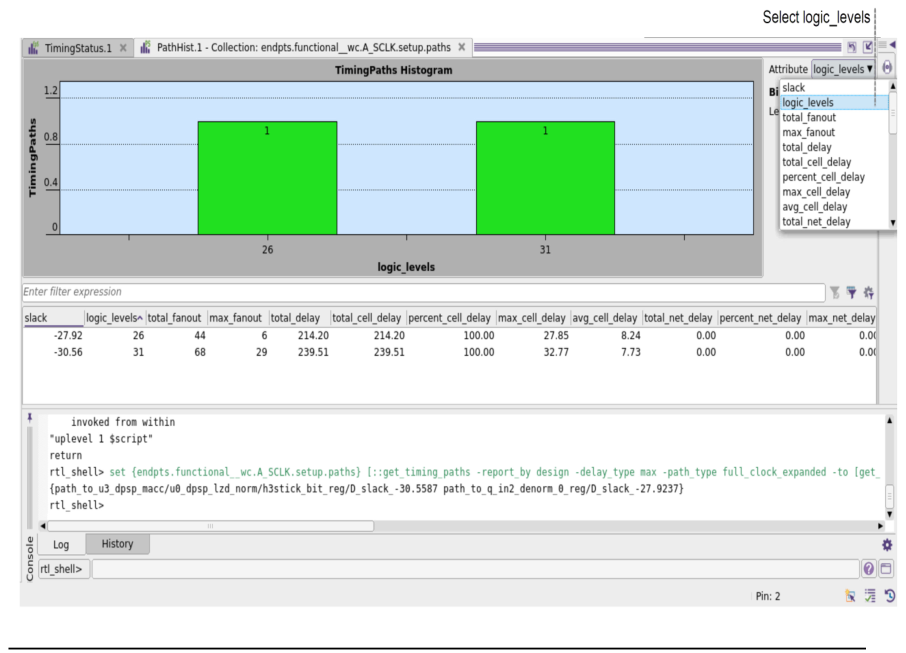
\includegraphics[width=0.85\textwidth]{gui-fig-127.png}
\caption{选择逻辑级数分析}
\label{fig:gui-127}
\end{figure}

\subsection{保存与加载时序路径数据}
\subsubsection*{Saving and Loading Timing Path Data}

要把所选时序路径集合存盘，在 Timing Analysis 窗口底部（Path Collections 选项卡）单击 Write。若保存时启用了片上参数变化（POCV），POCV 数据会与时序路径一起保存。要加载先前保存的数据，单击 Read。若已启用 POCV 且文件中含有 POCV 数据，加载时会一并恢复。

\section{分析时序路径集合}
\subsection*{Analyzing Timing Path Collections}

路径分析器（path analyzer）按你指定的规则分析一组时序路径，根据可用属性值分类，并在按颜色编码的 treemap 中显示各类。可以选择预定义分类规则，或定义自定义规则，也可以添加子类。

在时序分析窗口中选择 \textbf{View > New Path Analyzer} 打开路径分析器。

必须先加载并分类时序路径，才能在 treemap 中查看。

加载一组时序路径：
\begin{enumerate}
  \item 在 Collections 框中指定集合。可以输入集合名，或输入一条创建该集合的 Tcl 命令。
  \item 单击 Apply。
\end{enumerate}

对时序路径分类：
\begin{enumerate}
  \item 在分类树中选择 All。
  \item 单击 Create。出现 Create Category 对话框。
  \item 选择一条规则。
  \item 单击 OK。
\end{enumerate}

可以从同一设计加载一组或多组时序路径。

分类之后，选择分类树顶部的 All，并拖动右侧滑块，在 treemap 中查看各类。All 包含已载入路径分析器的全部路径。

\section{分析逻辑级数}
\subsection*{Analyzing Logic Levels}

在 GUI 中做逻辑级数分析时，路径集合窗口会更新时序路径的直方图，见图~\ref{fig:gui-128}。

\begin{figure}[htbp]
\centering
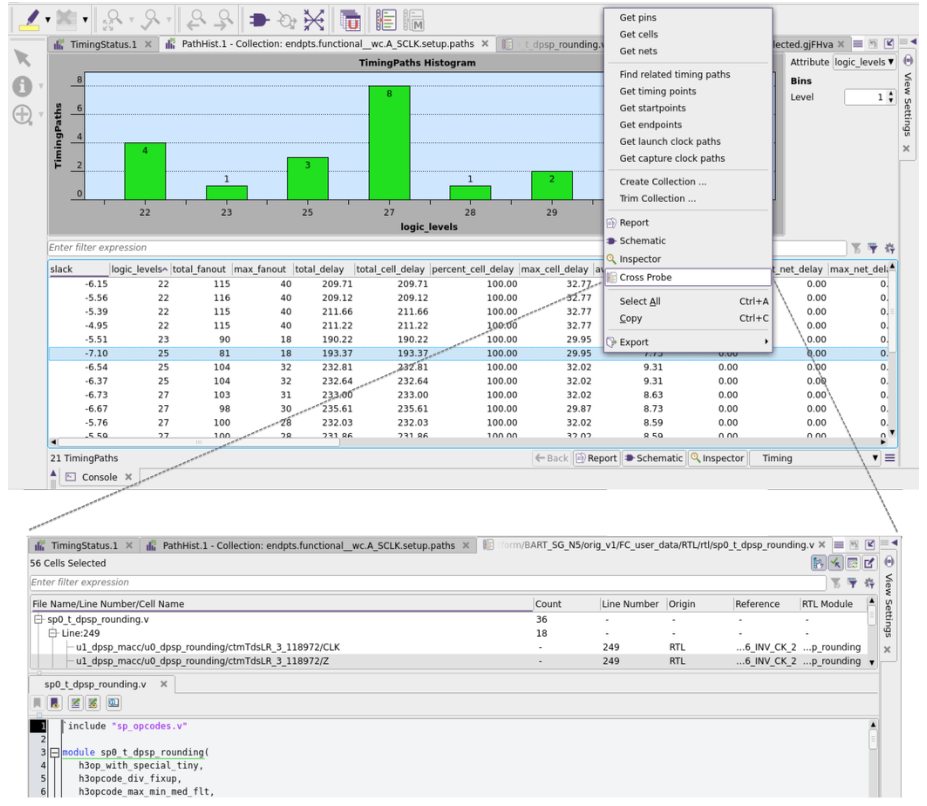
\includegraphics[width=0.92\textwidth]{gui-fig-128.png}
\caption{带逻辑级数的路径集合窗口}
\label{fig:gui-128}
\end{figure}

在端点裕量表中选中一条路径后打开上下文菜单，可以进一步查看，例如显示所选路径的原理图，或用 Cross Probe 显示对应的 RTL。相关入口见图~\ref{fig:gui-129}。

\begin{figure}[htbp]
\centering
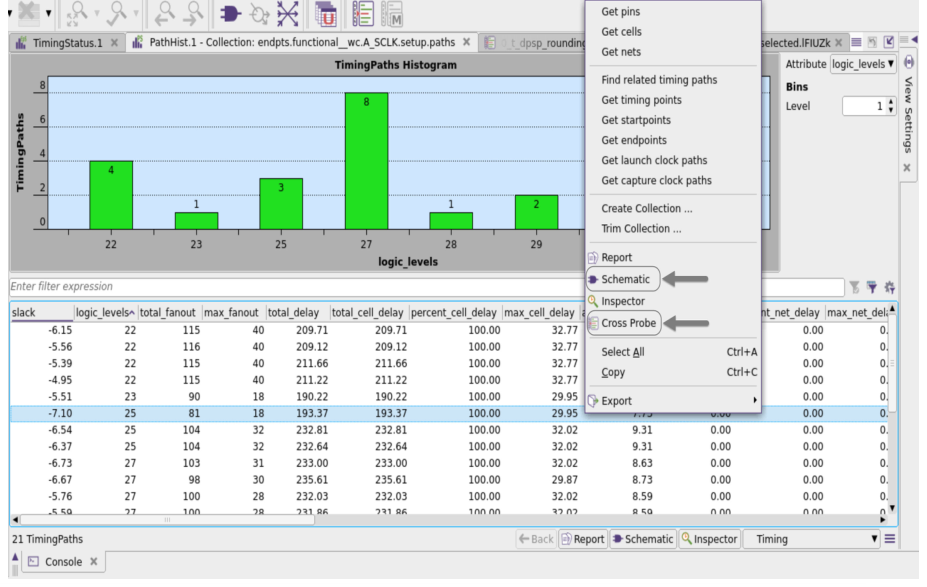
\includegraphics[width=0.7\textwidth]{gui-fig-129.png}
\caption{进一步分析的入口}
\label{fig:gui-129}
\end{figure}

% 第 9 章 Using UPF and Power Analysis Tools
\bichapter{使用 UPF 与功耗分析工具}{Using UPF and Power Analysis Tools}
\label{chap:gui-upf}

对多电压设计，IC Compiler II GUI 提供 UPF 查看器、功耗状态表视图以及其他工具，用于查看设计的 UPF 功耗意图并支持分析。

本章包括以下主题：
\begin{itemize}
  \item 查看 UPF 功耗意图
  \item 查看功耗状态表
\end{itemize}

\section{查看 UPF 功耗意图}
\subsection*{Viewing the UPF Power Intent}

UPF 图以图形表示设计的 UPF 功耗意图，显示电源域（power domain）、供电网络、电源开关、隔离与保持策略，以及功耗意图中的其他元素。UPF 图支持缩放、平移、对象选择和对象查询。

选择 \textbf{View > Multivoltage UPF > Power Domain / Root Cell}，或单击 Power Domain 按钮。图~\ref{fig:gui-130} 同时显示版图、UPF 图和视图设置。

\begin{figure}[htbp]
\centering
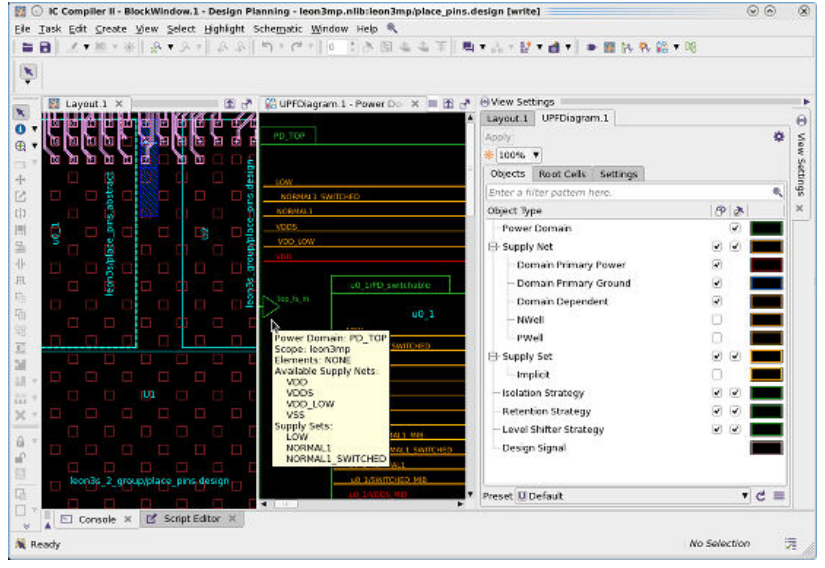
\includegraphics[width=0.92\textwidth]{gui-fig-130.png}
\caption{UPF 图视图}
\label{fig:gui-130}
\end{figure}

\subsection{电源域视图}
\subsubsection*{Power Domain View}

首次打开 UPF 图时，工具在电源域视图中显示 power scope 层次。信息按电源域层次组织。顶层电源域内的电源域显示为顶层的子模块。单击某个电源域即可选中它；右键可以选择相关单元、宏单元或 voltage area，也可以显示供电网络视图或功耗状态表。

每个电源域的供电集（supply set）画在矩形靠近顶部的位置；每条粗橙线代表一个唯一的供电集。单击该线即可选中。右键打开上下文菜单，选择 Show Supply Network View 或 Power State Table，可查看该供电集的更多信息。供电集下方是供电网络（supply net），每条细橙线代表一条供电网络。

用缩放和平移工具浏览视图，用方向键上下左右滚动。用选择工具点选单个对象，或框选矩形区域内的对象。指针停在对象上可在信息提示中预览；用 Query 工具可把对象信息显示在 Query 面板中。

在 View Settings 菜单中单击 UPFDiagram 选项卡，可查看电源域视图里对象类型与颜色的对应关系。单击色块可定制该对象类型的颜色。

若存在隔离单元，它们显示在供电网络下方。指针停在隔离单元上可在信息提示中看到更多信息。单击该线选中它，或右键打开上下文菜单，用以选择相关对象，或显示供电网络视图与功耗状态表。地网画在底部，每条细蓝线代表一条地网。

端口沿电源域边界显示。输入端口标为 I，输出端口标为 O。

\subsection{供电网络视图}
\subsubsection*{Supply Network View}

供电网络视图是电源域的另一种看法，显示不同电源域、隔离单元、开关单元以及电源域中其他元素之间的连接。与电源域视图一样，它按 power scope 层次组织。在视图中任意位置右键并选择 Show Supply Network View，即可显示图~\ref{fig:gui-131}。

\begin{figure}[htbp]
\centering
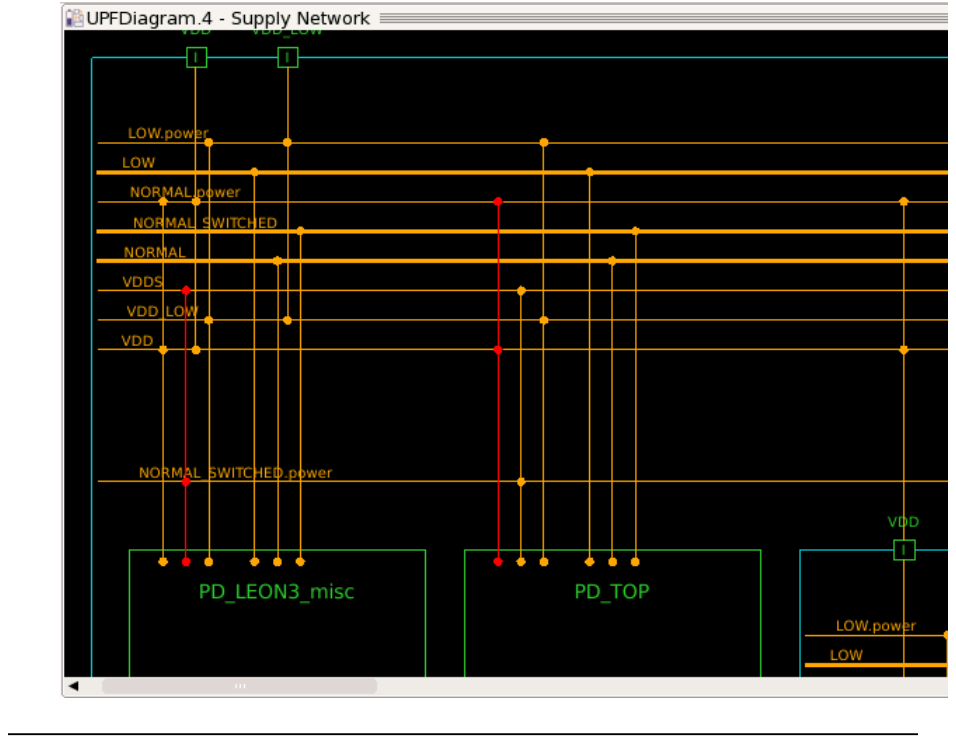
\includegraphics[width=0.92\textwidth]{gui-fig-131.png}
\caption{供电网络视图}
\label{fig:gui-131}
\end{figure}

\section{查看功耗状态表}
\subsection*{Viewing the Power State Table}

Power State Table 面板可与 UPF 图一起用来分析和调试隔离策略与电平移位策略。工具在功耗状态表中显示每路供电的状态，并在 UPF 图中显示它们的关系。面板见图~\ref{fig:gui-132}。

\begin{figure}[htbp]
\centering
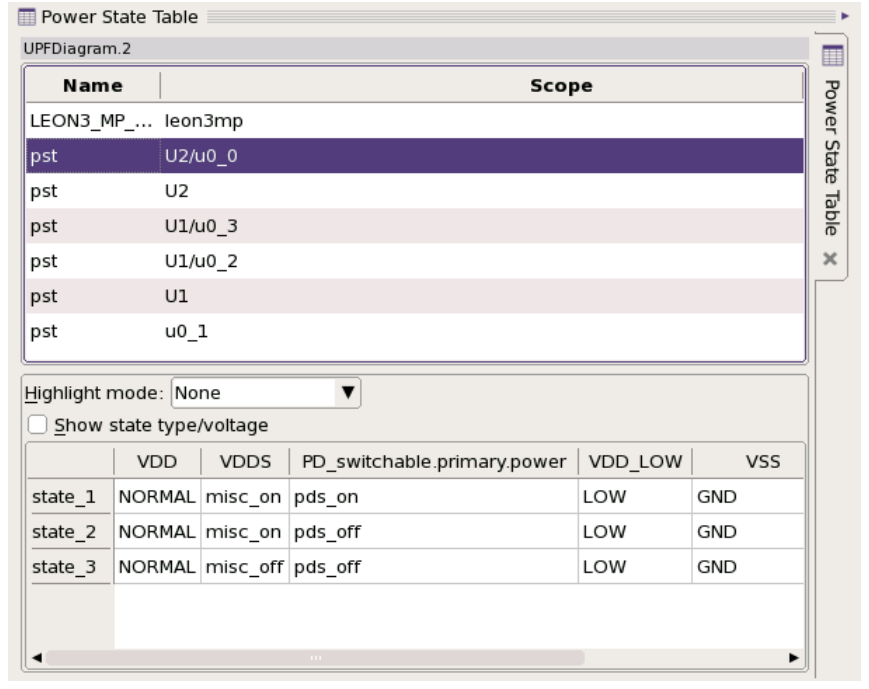
\includegraphics[width=0.92\textwidth]{gui-fig-132.png}
\caption{功耗状态表}
\label{fig:gui-132}
\end{figure}

该面板支持下列分析类型：
\begin{itemize}
  \item Always-on 分析比较电源与地之间的通断状态，结果为 More AO、Less AO、Equally AO 或 Unrelated AO 之一。
  \item 多电压电平移位分析比较各路电源之间的电压关系，结果为 LH（低到高）、HL（高到低）、HL\_LH（高低双向）或 None 之一。
\end{itemize}

% 第 10 章 Using the Error Browser
\bichapter{使用错误浏览器}{Using the Error Browser}
\label{chap:gui-error}

IC Compiler II GUI 提供错误浏览器（error browser）工具，用于查看错误消息和信息性消息（informational message），在版图视图（layout view）中高亮相关对象，并处置（disposition）错误。使用错误浏览器可以快速选出一组待复查的错误，定位某一条特定错误，并在版图中调查该问题。

本章包括以下主题：
\begin{itemize}
  \item 错误浏览器概述
  \item 加载与保存错误数据
  \item 管理错误层次
  \item 管理错误列表并查看错误详情
  \item 使用错误过滤器
  \item 高亮错误
  \item 将错误标记为已修复并更改错误状态
  \item 写出设计规则检查（DRC）错误数据
\end{itemize}

\section{错误浏览器概述}
\subsection*{Error Browser Overview}

错误浏览器提供若干功能，帮助复查错误、处置错误，并把更新后的错误文件保存到磁盘。在错误浏览器中选中错误时，版图查看器（layout viewer）会平移到错误所在位置并放大，以便在视图中单独观察该错误。

\begin{noteBox}
错误浏览器缩放或平移以显示所选错误时，只有活动版图视图会随之改变。
\end{noteBox}

错误浏览器按错误类型（error type）把错误归组。错误类型由生成该错误的 GUI 任务或 Tcl 命令指定。每条错误包含简短描述、该错误的包围盒（bounding box）坐标，以及关于该错误的其他信息。

要启动错误浏览器，选择 \textbf{View > Error Browser}。第一次打开错误浏览器时，工具会显示一个对话框，其中列出可用的错误消息文件、生成该文件的检查任务（checking task），以及文件上次被修改的时间。在列表中选择一项，然后单击 Open Selected 继续。错误浏览器见图~\ref{fig:gui-133}。

\begin{figure}[htbp]
\centering
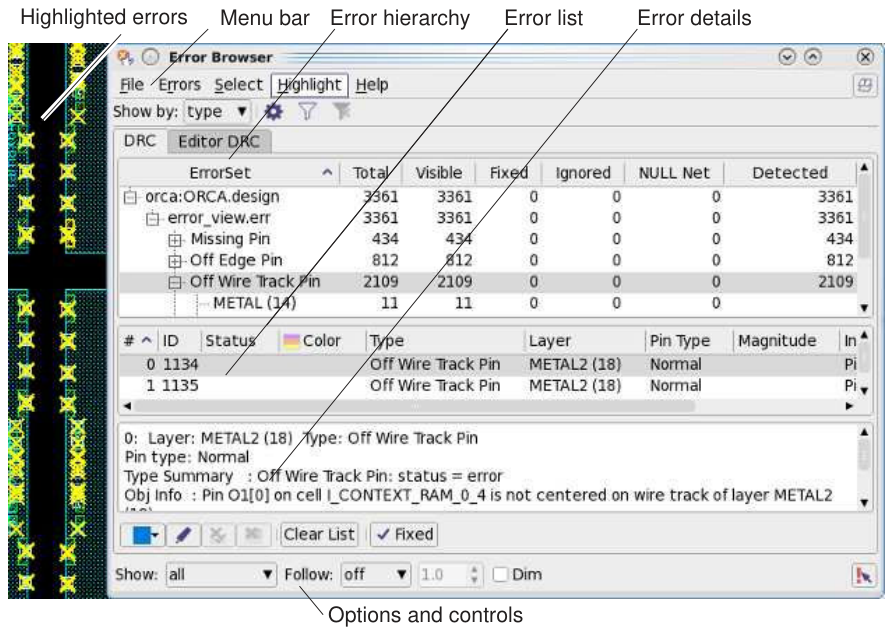
\includegraphics[width=0.92\textwidth]{gui-fig-133.png}
\caption{错误浏览器}
\label{fig:gui-133}
\end{figure}

用错误浏览器调试错误的典型流程包括以下步骤：
\begin{enumerate}
  \item 验证设计并保存结果。
  \item 在错误浏览器中打开已保存的错误文件。
  \item 选择一组要复查的错误。\\
        可以按错误类型分组，也可以按与这些错误关联的层（layer）分组。还可以按错误在设计中的物理位置选择一组错误。
  \item 在列表中选中错误，并在版图视图中查看错误的上下文，从而逐条分析并调试。
  \item 在版图视图中改正错误，并在错误浏览器中把该错误标为已修复（fixed）或已忽略（ignored）。
  \item （可选）隐藏已修复的错误。
\end{enumerate}

\section{加载与保存错误数据}
\subsection*{Loading and Saving Error Data}

默认情况下，错误浏览器读取并写入与当前块（block）关联的错误数据（error data）文件。这些文件使用 \cmd{.err} 扩展名，保存在该块的库目录（library directory）中。也可以保存和加载不与该块关联的 XML 格式错误数据文件。

要打开与当前块关联的已有错误数据文件：
\begin{enumerate}
  \item 选择 \textbf{File > Open}，打开 Open Error Data 对话框。
  \item 选择要打开的错误数据文件。
  \item 单击 Open Selected 按钮。
\end{enumerate}

要打开扩展名为 \cmd{.err} 的错误数据文件，或非托管的 XML 格式错误数据文件：
\begin{enumerate}
  \item 选择 \textbf{File > Read Error File}，打开文件浏览器。
  \item 选择要打开的文件。\\
        若文件扩展名为 \cmd{.xml}，请在 Open Error Data File 对话框的 Files of type 框中选择 Any files。
  \item 单击 OK。
\end{enumerate}

更新已修复状态或做了其他更改之后，要保存对错误数据的更改：
\begin{enumerate}
  \item 选择 \textbf{File > Save}。
  \item 单击 Save 按钮。
\end{enumerate}

工具把错误浏览器的当前状态写入输出文件。若没有打开的错误数据文件，或者错误数据没有更改，该菜单操作处于禁用状态。

要以其他格式保存错误数据：
\begin{itemize}
  \item 选择 \textbf{File > Export as CSV}，把错误数据写成逗号分隔值（comma-separated values，CSV）。
  \item 选择 \textbf{File > Export to Error File}，把这些信息写成错误数据。
\end{itemize}

\section{管理错误层次}
\subsection*{Managing the Error Hierarchy}

错误浏览器在菜单栏下方显示两个选项卡：DRC 与 Editor DRC。DRC 选项卡中的列表显示当前错误数据文件里的错误层次（error hierarchy）。可以对错误层次列表执行下列操作：
\begin{itemize}
  \item 单击 ErrorSet 列左侧的 [+] 按钮展开列表，或单击 [-] 按钮折叠列表。
  \item 单击列标题，对该列排序，或更改该列的排序方向。
  \item 把指针移到列表中的某一行上，在信息提示（infotip）中显示信息。
  \item 单击列表中的某一行，在版图视图中平移并缩放到该错误，并在浏览器的错误列表区域显示更多信息。
  \item 单击某一行，按住 Shift 键，再单击列表中更靠下的另一行，以选中这一范围内的各行。
  \item 单击某一行，按住 Ctrl 键，再单击第二行，以选中多行。继续按住 Ctrl 键并单击其他行，把它们加入选择。
  \item 右键单击鼠标，显示上下文菜单（context menu）；从菜单中选择一项，可以打开新的错误数据、保存当前错误数据、把当前错误标为已修复，以及执行其他同类操作。
  \item 从错误浏览器菜单选择 \textbf{Errors > Next Error Group} 或 \textbf{Errors > Previous Error Group}，转到错误层次中的另一个错误组。
\end{itemize}

\section{管理错误列表并查看错误详情}
\subsection*{Managing the Error List and Viewing Error Details}

在错误层次列表下方，工具显示错误列表（error list）。错误列表列出你在工具的错误层次区域中所选错误类型下的各条错误。可以对错误列表执行下列操作：
\begin{itemize}
  \item 单击列标题，对该列排序，或更改该列的排序方向。
  \item 单击并拖动列标题，以调整各列的顺序。
  \item 把指针移到列表中的某一行上，在信息提示中显示信息。
  \item 单击列表中的某一行，在版图视图中平移并缩放到该错误，并在浏览器的错误列表区域显示更多信息。
  \item 右键单击鼠标，显示上下文菜单；从菜单中选择一项，可以切换该错误的已修复状态、高亮错误，以及执行其他同类操作。
  \item 按住 Ctrl 或 Shift 键并单击列表中的其他行，或沿列表向下单击并拖动鼠标，以选择多条错误。
  \item 选择上下文菜单中的相应项，或选择 \textbf{Errors > Clear Error List}，清空该列表。
  \item 从错误浏览器菜单选择 \textbf{Errors > Next Error Group} 或 \textbf{Errors > Previous Error Group}，转到错误列表中的另一组。
\end{itemize}

错误浏览器在错误列表下方的错误详情（error detail）区域显示所选错误的详情。把指针停在错误详情窗格上，会显示包含错误详情的信息提示。

\section{使用错误过滤器}
\subsection*{Using Error Filters}

使用错误过滤，可以暂时把错误从错误浏览器和版图视图中去掉。通过 Set Error Data Filter 对话框应用过滤器（filter），见图~\ref{fig:gui-134}。

要创建错误过滤器：
\begin{enumerate}
  \item 选择 \textbf{Errors > Set Filter}。
  \item 选择 Show only matching errors 或 Hide matching errors，以设置过滤器类型。
  \item 选择错误类型、层设置、线网（net）以及其他设置，从而建立过滤条件。
  \item 单击 Apply 或 OK 以应用过滤器，或单击 Clear Filter 以去掉过滤器。
\end{enumerate}

创建过滤器之后，该过滤器会作用于当前已经打开的错误数据，以及在当前会话中打开的任何其他错误数据。过滤器不会累积；应用新的过滤器会覆盖此前设置的任何过滤器。要清除过滤器，选择 \textbf{Errors > Clear Filter}，或在 Set Error Data Filter 对话框中单击 Clear Filter。

\begin{figure}[htbp]
\centering
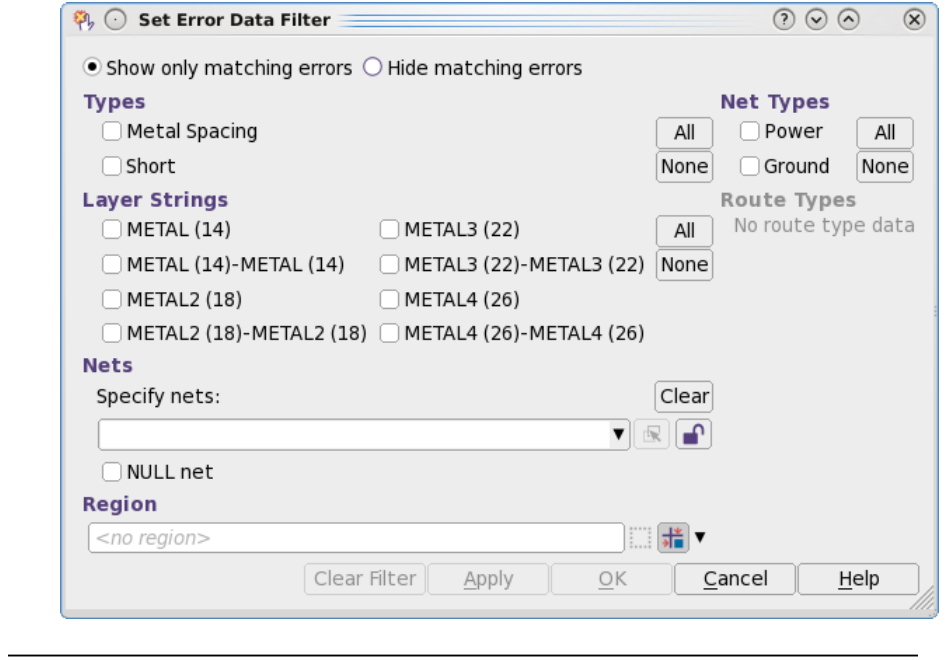
\includegraphics[width=0.92\textwidth]{gui-fig-134.png}
\caption{Set Error Data Filter 对话框}
\label{fig:gui-134}
\end{figure}

\section{高亮错误}
\subsection*{Highlighting Errors}

可以给版图视图中的错误加上不同的高亮（highlight）颜色。使用 Highlight 菜单来高亮错误，或去掉高亮。也可以使用 GUI 底部的高亮按钮完成这些操作。Highlight 菜单提供下列菜单命令：
\begin{itemize}
  \item By Type, Layer, Net：打开 Highlight Errors 对话框，按错误类型、层字符串（layer string）或关联线网高亮错误。
  \item Selected：用当前高亮颜色高亮所选错误。
  \item All Errors in List：用当前高亮颜色高亮错误列表中的全部可见错误。
  \item Clear Selected：清除所选错误上的高亮颜色。
  \item Clear Current Color：清除当前高亮颜色的全部高亮。
  \item Clear All：清除全部错误高亮。
  \item Set Current Color：提供颜色菜单，用来选定当前高亮颜色。
  \item Next Color：把当前高亮颜色切换为 Set Current Color 菜单中的下一种颜色。
  \item Auto Cycle Colors：切换此选项。启用后，每执行一次 \textbf{Highlight > Selected}，当前高亮颜色就改为下一种颜色。
  \item Error Highlight Counts：打开一个对话框，显示每个高亮集合中的错误数量，以及一张简单直方图（histogram）。
\end{itemize}

\section{将错误标记为已修复并更改错误状态}
\subsection*{Marking Errors as Fixed and Changing Error Status}

要更改某条错误的状态，先在错误列表中选择一条或多条错误，然后执行下列操作之一：
\begin{itemize}
  \item 单击 Fixed 按钮，切换 Status 列中的已修复状态值。
  \item 单击鼠标右键并选择 Set Status，然后按需要选择 Error、Fixed 或 Ignored。也可以从错误浏览器菜单选择 \textbf{Errors > Set Status}，并做相同的选择。
\end{itemize}

这些操作会更改所选错误的状态。Status 列中的值变为对勾，表示该错误已修复；该标记被清除，表示错误尚未修复；变为 (X)，表示处于已忽略状态。

\section{写出设计规则检查（DRC）错误数据}
\subsection*{Writing Out DRC Error Data}

错误浏览器提供图形工具，用来复查工具中各条检查命令所报告的错误。要把某个错误数据文件中的错误写成文本报告，使用 \cmd{report\_drc\_errors} 命令，并用选项报告特定的错误类型，或报告特定层上的错误。

该命令可以写出下列类型的报告：\cmd{error\_type}、\cmd{error\_layer}、\cmd{detailed} 和 \cmd{matrix}。使用 \opt{-report\_type} 选项指定报告类型。\cmd{error\_type} 报告是默认报告类型，不指定选项时就会生成，也可以通过指定 \opt{-report\_type error\_type} 生成。它列出每种错误类型及其计数，如下例所示。\cmd{error\_layer} 报告由 \opt{-report\_type error\_layer} 选项生成，与 \cmd{error\_type} 报告类似，但先按层分组，再按错误类型分组。

\begin{lstlisting}
ErrorSet                                 Total  Visible  Fixed  Ignored
-----------------------------------------------------------------------
Design : test                            54     3        0      0
      Data : zroute.err                  54     3        0      0
            Net                          3      1        0      0
                METAL3 (28)              1      1        0      0
            Route Spacing                6      2        0      0
                METAL2 (18)-METAL3 (28)  1      1        0      0
                METAL3 (28)-METAL4 (31)  1      1        0      0
\end{lstlisting}

\cmd{detailed} 报告由 \opt{-report\_type detailed} 选项生成。它为每条错误报告错误标识（error ID）、错误类型以及其他信息，内容与错误浏览器中显示的完整错误信息类似。详细报告如下例所示。

\begin{lstlisting}
Error ID          : 1
Error Type        : Route Spacing
Error Layer       : METAL3 (28)-METAL4 (31)
Number of errors  : 6
Description       : Spacing violation between
                    hmg_out44_10_ and RES_I109_X9
                    on layers {METAL3 (28) METAL4 (31)} --
                    direction: vertical, required: 1.2 um, actual: 0.6 um
Status            : error
Bbox              : {293.8000 364.4000} {294.2000 366.8000}

Error ID          : 3
Error Type        : Route Spacing
Error Layer       : METAL2 (18)-METAL3 (28)
Number of errors  : 6
Description       : Spacing violation between A0_9_ and
                    B0_9_ on layers {METAL2 (18) METAL3 (28)} --
                    direction: upper left to lower right, required:
                    1.2000 um, actual: 0.6000 um
Status            : error
Bbox              : {261.0000 301.8000} {261.4000 303.0000}
\end{lstlisting}

下列示例按所用的命令选项写出不同的错误报告：
\begin{itemize}
  \item 为错误数据文件中的全部错误写出默认的 \cmd{error\_data} 错误报告。
\end{itemize}
\begin{lstlisting}
icc2_shell> report_drc_errors -error_data zroute.err
\end{lstlisting}
\begin{itemize}
  \item 只为 METAL3 层上、错误类型为 Route Spacing 和 Net 的错误写出详细报告。
\end{itemize}
\begin{lstlisting}
icc2_shell> set type [get_drc_error_types \
   -error_data zroute.err {{Route Spacing} {Net}}]
icc2_shell> report_drc_errors -error_data zroute.err \
   -report_type detailed -error_type $type -layers {METAL3}
\end{lstlisting}

% 第 11 章 Using the Message Browser
\bichapter{使用消息浏览器}{Using the Message Browser}
\label{chap:gui-msg}

IC Compiler II GUI 提供增强消息系统（enhanced message system，EMS）数据库以及消息浏览器（message browser）工具，用来管理和查看与版图中规则违例（rule violation）有关的错误消息和信息性消息（informational message）。EMS 数据库由 \cmd{check\_design} 命令以及其他检查命令生成。使用消息浏览器时，可以选中单条消息，也可以按消息类型选择消息，在版图视图（layout view）中高亮受影响的对象，并为违例创建豁免（waiver）。消息浏览器还会为当前选中的消息显示 HTML 格式的手册页（man page）。如果有多个 EMS 数据库，消息浏览器可以把这些数据库合并成一个统一的数据库。

本章包括以下主题：
\begin{itemize}
  \item 准备 EMS 数据库
  \item 消息浏览器布局
  \item 重新分类消息
  \item 创建豁免
  \item 合并 EMS 数据库
\end{itemize}

\section{准备 EMS 数据库}
\subsection*{Preparing the EMS Database}

使用消息浏览器之前，必须先创建 EMS 数据库。

该数据库由设计检查工具生成，例如 \cmd{check\_design}、\cmd{check\_hier\_design}、\cmd{check\_netlist}、\cmd{check\_routability} 和 \cmd{check\_timing}。在检查命令之前运行 \cmd{create\_ems\_database} 命令，在检查命令之后运行 \cmd{save\_ems\_database} 命令。例如：
\begin{lstlisting}
icc2_shell> create_ems_database check_hier.ems
icc2_shell> check_hier_design -stage timing
icc2_shell> save_ems_database
\end{lstlisting}

在版图窗口中选择 \textbf{Window > Message Browser Window}，打开消息浏览器。也可以在 \cmd{check\_design} 命令上加上 \opt{-open\_message\_browser} 选项，使分析结束后自动打开消息浏览器。

\section{消息浏览器布局}
\subsection*{Message Browser Layout}

图~\ref{fig:gui-135} 标出了消息浏览器中的各个区域。

\begin{figure}[htbp]
\centering
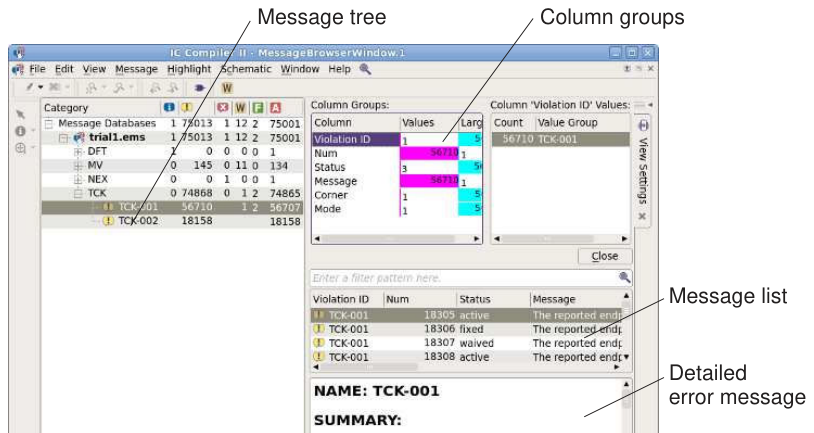
\includegraphics[width=0.92\textwidth]{gui-fig-135.png}
\caption{消息浏览器}
\label{fig:gui-135}
\end{figure}

以下几节说明消息浏览器中的各个窗格。

\subsection{消息树}
\subsubsection*{Message Tree}

消息树在浏览器左侧以树视图（tree view）列出错误，见图~\ref{fig:gui-136}。树视图显示当前 EMS 数据库的名称，以及数据库中错误与警告的层次。

\begin{figure}[htbp]
\centering
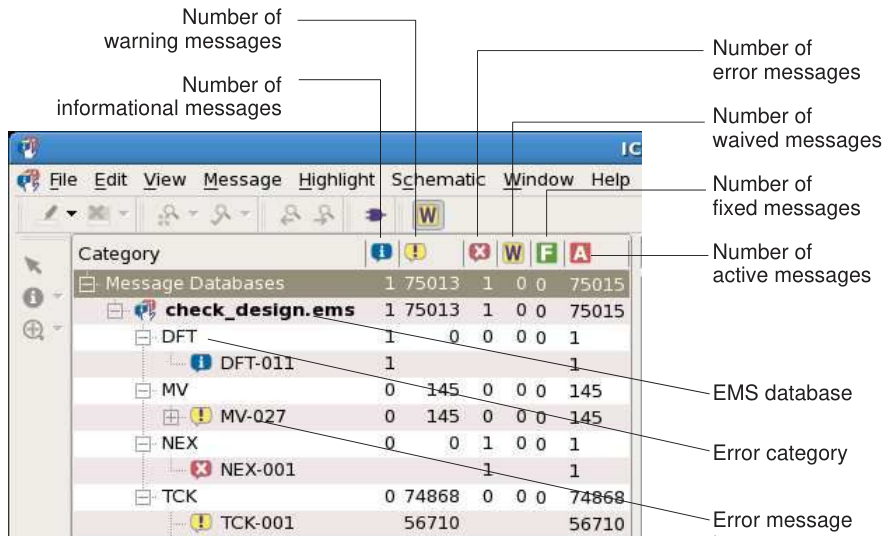
\includegraphics[width=0.92\textwidth]{gui-fig-136.png}
\caption{消息浏览器树}
\label{fig:gui-136}
\end{figure}

\subsection{消息列表}
\subsubsection*{Message List}

消息列表显示当前所选错误消息类型的完整消息列表，见图~\ref{fig:gui-137}。每个条目包括违例标识（Violation ID）、内部错误消息索引、当前状态（活动 active、已豁免 waived 或已修复 fixed）、消息文本，以及在有附加信息时一并给出的内容。把鼠标指针移到某一消息行上，可以查看该消息的更多信息。单击列表中的一行即可选中它。选中消息行之后，工具会更新详细错误消息的显示。单击并拖动指针可以选中多行；也可以在单击某一行时按住 Shift 或 Control 键，把该行加入选择。按 Control-A 选中全部行。

\begin{figure}[htbp]
\centering
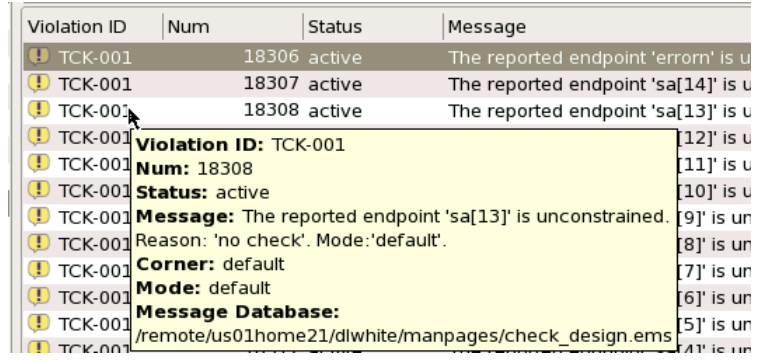
\includegraphics[width=0.92\textwidth]{gui-fig-137.png}
\caption{消息列表}
\label{fig:gui-137}
\end{figure}

在消息区域单击鼠标右键，显示上下文菜单（context menu）；从菜单中选择一项，可以执行下列操作：
\begin{itemize}
  \item Waive：把所选消息重新分类为已豁免；此操作只在当前会话中保留。
  \item Mark Fixed：把所选消息重新分类为已修复；此操作只在当前会话中保留。
  \item Mark Active：把所选消息重新分类为活动；此操作只在当前会话中保留。
  \item Select：在版图视图中选中相关对象。
  \item Highlight：在版图视图中高亮相关对象。
  \item Properties：显示该对象的属性。
  \item Show Column Groups：打开 Column Groups 窗格和 Column Status Values 窗格。
  \item Create Waiver：打开 Create Waiver 对话框；用该对话框创建豁免，见后文「创建豁免」。
  \item List Waivers：打开 Message Waivers 对话框；用该对话框显示当前的豁免列表。
  \item Copy：复制当前所选行的文本。
\end{itemize}

可以输入过滤模式，或使用列分组（column group）来过滤消息列表。在搜索框中输入字符时，工具会更新显示，只列出包含该搜索字符串的消息。

列分组把消息列表区域各列的信息计数组合成直方图（histogram）视图。数值列显示每一列有多少个互不相同的结果。在 Column Groups 框中单击某一行，右侧的列值区域会显示更多信息。在列值区域中单击某一行时，消息列表被过滤，只显示与当前所选值分组相匹配的消息。单击 Close 按钮，关闭列分组面板。列分组见图~\ref{fig:gui-138}。

\begin{figure}[htbp]
\centering
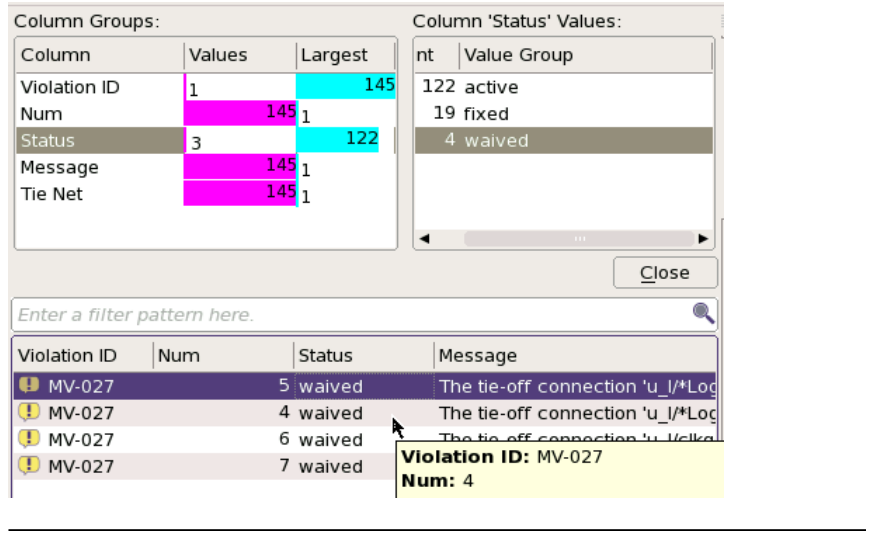
\includegraphics[width=0.92\textwidth]{gui-fig-138.png}
\caption{列分组}
\label{fig:gui-138}
\end{figure}

\subsection{详细错误消息}
\subsubsection*{Detailed Error Message}

消息浏览器显示当前所选错误的详细消息摘要和说明。在消息列表中单击不同的错误消息时，详细错误消息会显示该错误的消息摘要和详细说明。

要改变详细错误消息的位置，从菜单选择 \textbf{View > Html Pane}，然后选择 On Right 或 On Bottom。

\section{重新分类消息}
\subsection*{Reclassifying a Message}

使用消息浏览器，可以把单条消息重新分类为活动、已修复或已豁免。若只在当前会话中重新分类一条消息：
\begin{enumerate}
  \item 在树视图（Tree View）中选择该消息。
  \item 从 Message 菜单选择 Waive、Mark Fixed 或 Mark Active，见图~\ref{fig:gui-139}。也可以单击该消息，再从上下文菜单中选择相应操作。
\end{enumerate}
工具会更新列表视图中的计数。

\begin{figure}[htbp]
\centering
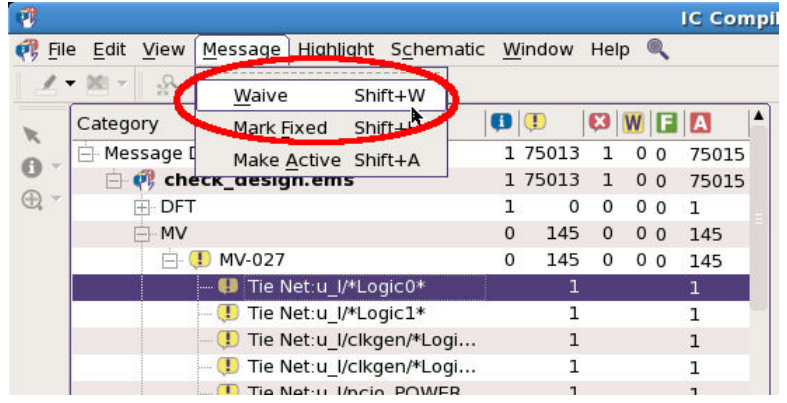
\includegraphics[width=0.92\textwidth]{gui-fig-139.png}
\caption{重新分类消息}
\label{fig:gui-139}
\end{figure}

\begin{noteBox}
这些更改只在当前会话中有效，退出消息浏览器时不会保存。
\end{noteBox}

\section{创建豁免}
\subsection*{Creating a Waiver}

为一条消息创建豁免，可以把附加信息关联到该消息上。这些信息不会保存到 EMS 数据库中。不过，可以把豁免写成 Tcl 命令，并在以后的会话中应用。要创建豁免：
\begin{enumerate}
  \item 选择要豁免的消息行。
  \item 右键单击，并从上下文菜单中选择 Create Waiver。\\
        工具在消息列表上方显示错误豁免表单（error waiver form），见图~\ref{fig:gui-140}。
  \item 在 Name 以及其他框中填写信息，完成错误豁免表单。标签前带星号（*）的框为必填项。
  \item 按需要修改条件（criteria）。\\
        单击加号按钮（+）添加条件，单击减号按钮（-）删除一条条件，或单击 Remove All 删除全部条件。
        \begin{noteBox}
        这些条件会应用于列表中的全部消息。
        \end{noteBox}
  \item 单击 Apply 创建豁免。\\
        工具把这些条件应用于列表中的全部消息，并把匹配消息的状态更新为 Waived。
\end{enumerate}

\begin{figure}[htbp]
\centering
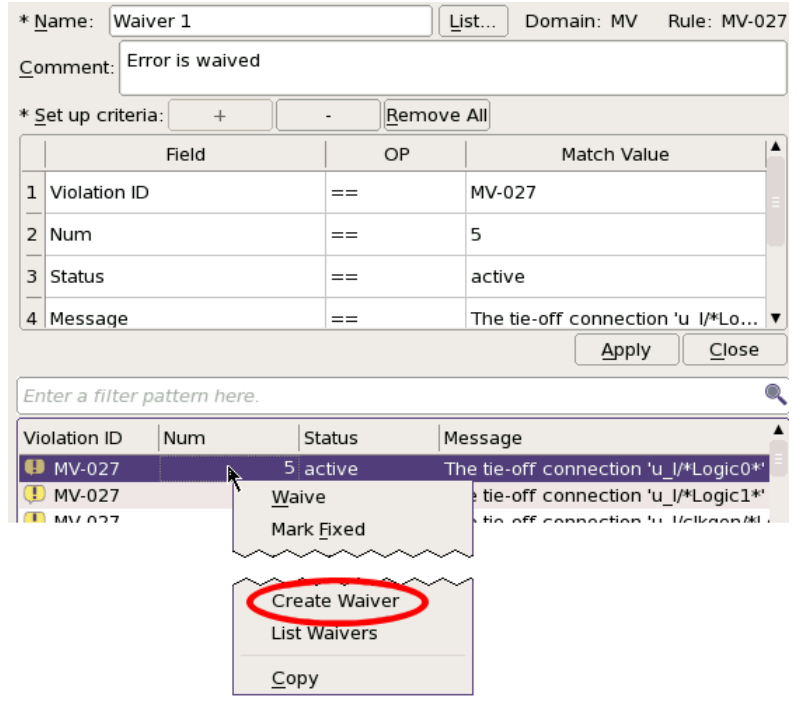
\includegraphics[width=0.92\textwidth]{gui-fig-140.png}
\caption{创建豁免}
\label{fig:gui-140}
\end{figure}

要显示当前会话的豁免列表，从菜单选择 \textbf{View > List Message Waivers}。工具会列出当前的豁免，见图~\ref{fig:gui-141}。

\begin{figure}[htbp]
\centering
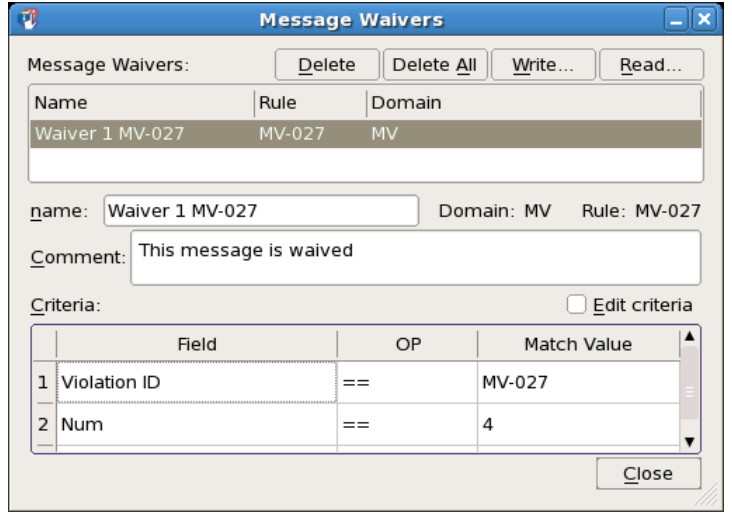
\includegraphics[width=0.92\textwidth]{gui-fig-141.png}
\caption{消息豁免列表}
\label{fig:gui-141}
\end{figure}

单击某一条豁免，可以查看创建该豁免时使用的条件。要编辑该豁免，选择 Edit criteria，修改条件设置，然后单击 Commit。也可以用这个对话框把当前豁免写成 Tcl 文件、读入保存在 Tcl 文件中的豁免，或删除当前豁免。

要在另一个会话中使用这些豁免，必须先把它们保存到磁盘。要把豁免保存到磁盘，在 Message Waivers 对话框中单击 Write，或从消息浏览器菜单选择 \textbf{File > Write Waiver to Script}。工具把 \cmd{gui\_create\_message\_waiver} 命令写入该文件。要读入保存在 Tcl 文件中的豁免，在 Message Waivers 对话框中单击 Read，或从消息浏览器菜单选择 \textbf{File > Read Waiver from Script}，然后选择包含这些豁免的 Tcl 文件。

\section{合并 EMS 数据库}
\subsection*{Merging EMS Databases}

消息浏览器可以在同一次会话中加载多个 EMS 数据库。同一时间只能有一个数据库处于活动状态。要加载不止一个数据库：
\begin{enumerate}
  \item 从菜单选择 \textbf{File > Open Message Database}。\\
        也可以用 \cmd{open\_ems\_database} 这条 Tcl 命令打开数据库，如下例所示：
\begin{lstlisting}
icc2_shell> open_ems_database MV.ems
\end{lstlisting}
  \item （可选）若已经打开多个 EMS 数据库，单击要合并的那个数据库以选中它，并从菜单选择 \textbf{File > Set Current Message Database}。
  \item 从菜单选择 \textbf{File > Merge Message Database}，选择一个文件，然后单击 OK。
\end{enumerate}

工具加载所选的数据库文件，并把它设为当前数据库，见图~\ref{fig:gui-142}。新加载的数据库文件既包含它自己原有的消息，也包含合并之前当前数据库中的消息。

\begin{figure}[htbp]
\centering
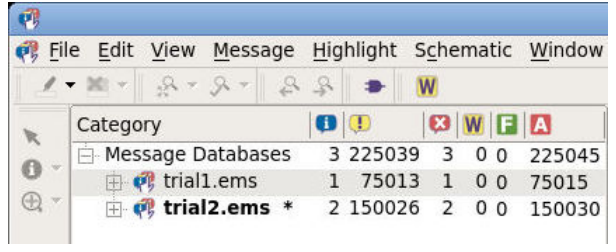
\includegraphics[width=0.92\textwidth]{gui-fig-142.png}
\caption{合并数据库}
\label{fig:gui-142}
\end{figure}

\begin{seeAlsoBox}
用 Tcl 命令管理 EMS 数据库的更多信息，见下列命令的手册页：
\begin{itemize}
  \item \cmd{close\_ems\_databases}
  \item \cmd{create\_ems\_database}
  \item \cmd{get\_current\_ems\_database}
  \item \cmd{get\_ems\_databases}
  \item \cmd{open\_ems\_database}
  \item \cmd{save\_ems\_database}
  \item \cmd{set\_current\_ems\_database}
\end{itemize}
\end{seeAlsoBox}

% 第 12 章 Creating Charts
\bichapter{创建图表}{Creating Charts}
\label{chap:gui-chart}

IC Compiler II 工具包含一套完整的绘图生成功能，可根据设计、版图及其他数据生成交互式绘图（plot）。更多信息见下列主题：
\begin{itemize}
  \item 创建模型
  \item 创建绘图
\end{itemize}

\section{创建模型}
\subsection*{Creating a Model}

要创建图表（chart），先从逗号分隔值（comma-separated values，CSV）文件导入图表数据，以创建模型（model）。使用 \cmd{gui\_create\_charts\_model} 命令读取 CSV，并把信息保存为 Tcl 变量。

下例写出一个简单的 CSV 文件，其中包含设计里每个宏单元（macro）的实例名、管脚数和面积。\cmd{gui\_create\_charts\_model} 命令装入该 CSV 文件并创建图表模型。

\begin{lstlisting}
set macros [get_cells -hier -filter "design_type==macro"]
set csv_file /tmp/count_area.csv
echo "macro_inst,count,area" > $csv_file
foreach_in_collection c $macros {
  echo [get_object_name $c],[get_attribute $c number_of_pins],[get_attribute $c area] >> $csv_file
}
set model [gui_create_charts_model -csv $csv_file -first_line_header ]
\end{lstlisting}

\begin{noteBox}
\cmd{gui\_create\_charts\_model} 命令会自动推导每一列数据的数据类型（data type）。
\end{noteBox}

也可以用 GUI 导入 CSV 文件。在 View Settings 面板中单击 Charts 选项卡，再单击 Models 选项卡。单击 Create 按钮，打开 Load Model 对话框。输入文件名，并选择用于指定表头的选项。工具会显示数据预览，见图~\ref{fig:gui-143}。单击 OK 创建模型。

\begin{figure}[htbp]
\centering
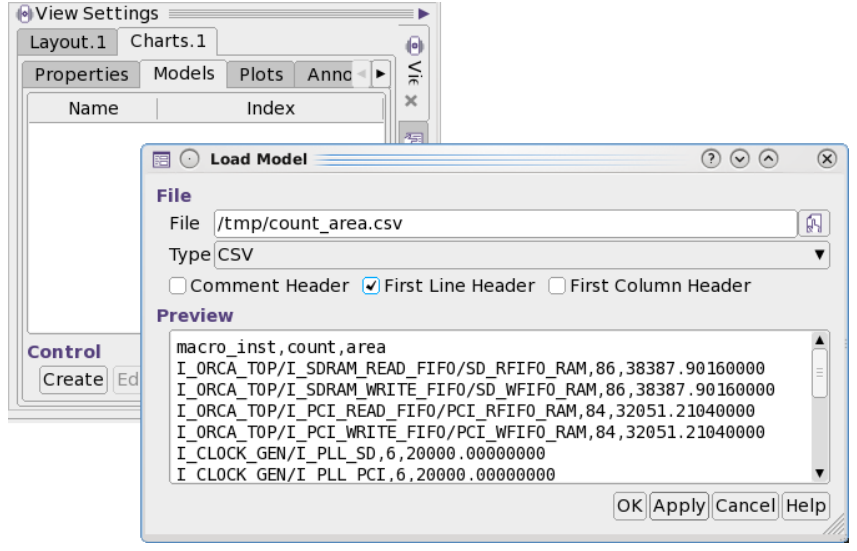
\includegraphics[width=0.92\textwidth]{gui-fig-143.png}
\caption{Load Model 对话框}
\label{fig:gui-143}
\end{figure}

除 CSV 之外，还可以直接从集合（collection）或 Tcl 数组（Tcl array）创建模型。例如：

\begin{lstlisting}
set selection [get_nets]
set model1 [gui_create_charts_model -clct $selection -columns {name dr_x_length dr_y_length}]

set data [list \
[list State {Under 5 Years} {5 to 13 Years} {14 to 17 Years} {18 to 24 Years} {25 to 44 Years} {45 to 64 Years} {65 Years and Over}] \
[list CA 2704659 4499890 2159981 3853788 10604510 8819342 4114496] \
[list TX 2027307 3277946 1420518 2454721 7017731 5656528 2472223] \
[list NY 1208495 2141490 1058031 1999120 5355235 5120254 2607672] \
[list FL 1140516 1938695 925060 1607297 4782119 4746856 3187797] \
[list IL 894368 1558919 725973 1311479 3596343 3239173 1575308] \
[list PA 737462 1345341 679201 1203944 3157759 3414001 1910571] \
]

set model2 [gui_create_charts_model -tcl $data -first_line_header]
\end{lstlisting}

\subsection{检查模型}
\subsubsection*{Checking the Model}

创建模型之后，在 GUI 中检查该模型：单击 View Settings 面板中的 Charts 选项卡。单击 Models 选项卡，显示用 \cmd{gui\_create\_charts\_model} 命令创建的模型列表。

要查看某个模型的详细信息，包括列名、数据类型和其他属性，在表中单击该模型，再单击 Edit 按钮，以显示数据表。单击每一列，可显示该数据列的列名、数据类型和其他属性。要更改该列的属性，在 Column Data 区域中选择一项，再单击 Apply。

\begin{figure}[htbp]
\centering
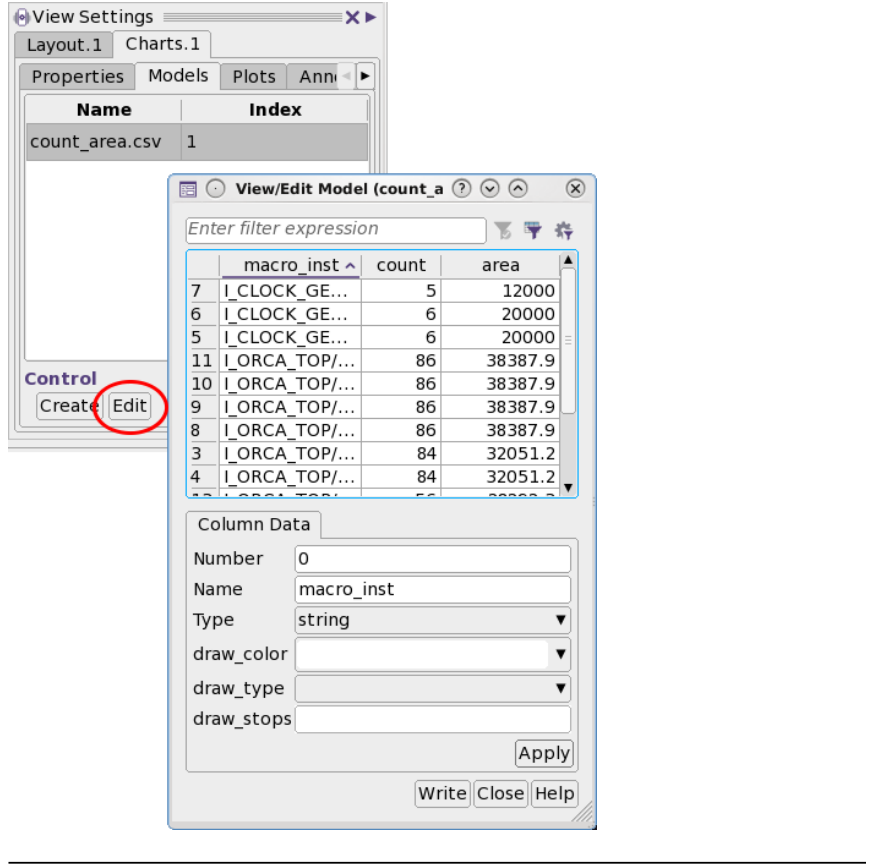
\includegraphics[width=0.92\textwidth]{gui-fig-144.png}
\caption{View/Edit Model 对话框}
\label{fig:gui-144}
\end{figure}

\subsection{向模型添加或删除数据}
\subsubsection*{Adding or Deleting Data From the Model}

导入 CSV 文件之后，可以用 \cmd{gui\_change\_charts\_model} 命令修改数据：添加列、删除列，以及执行其他操作。下例添加名为 \cmd{double\_count} 的新列，其值是 \cmd{column(1)} 中数据的两倍。

\begin{lstlisting}
gui_change_charts_model -model $model -add \
   -expr {column(1) + column(1)} -header double_count
\end{lstlisting}

\section{创建绘图}
\subsection*{Creating a Plot}

导入 CSV 文件并创建模型之后，可以创建绘图来查看数据。使用 \cmd{gui\_create\_charts\_plot} 命令创建条形图（bar chart）、分布图（distribution plot）、XY 图表（XY chart）等。

下例写出一个 CSV 文件，其中包含设计里四个宏单元的管脚数与面积。\cmd{gui\_create\_charts\_plot} 命令根据 CSV 文件的内容创建初始绘图。接着，从上下文菜单（context menu）中选择 Horizontal，把绘图转换成水平条形图。从上下文菜单中选择 Show Table，以显示数据表。

\begin{lstlisting}
# Create the Charts window
set view [gui_create_window -type Charts]

# Specify the macros and output CSV file
set macros [get_cells { cmem0/idata0_2/x0_t0 cmem0/dtags1_1/x0_t0
                        rf0/x0/t_bl cmem0/itags0_3/x0_t0 }]
set csv_file count_area.csv

# Write out the CSV file
echo "macro_inst,count,area" > $csv_file
foreach_in_collection c $macros {
  echo [get_object_name $c],\
[get_attribute $c number_of_pins],\
[get_attribute $c area] >> $csv_file
}

# Create the model
set model [gui_create_charts_model -csv $csv_file -first_line_header]

# Create the bar chart from the model
set plot [gui_create_charts_plot -view $view -type barchart \
   -model $model -columns {{name 0} {value {1}}}]
\end{lstlisting}

\begin{figure}[htbp]
\centering
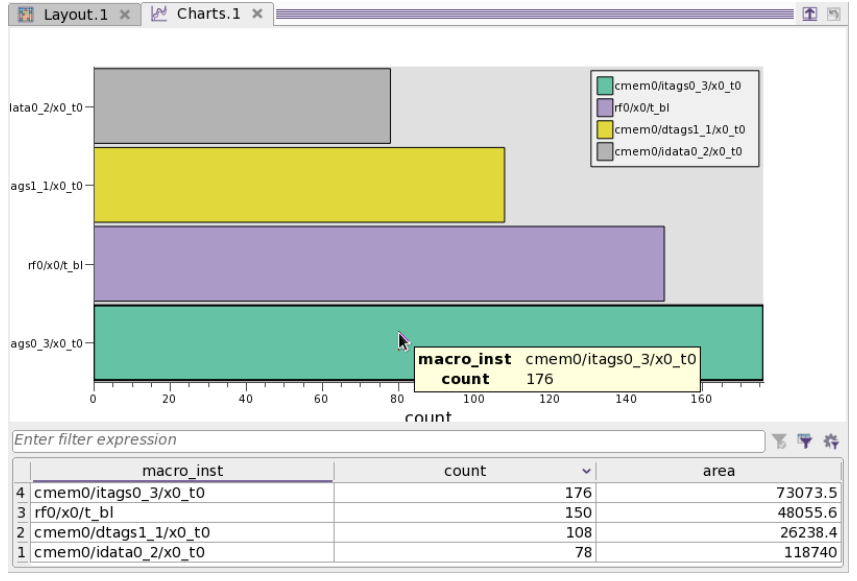
\includegraphics[width=0.92\textwidth]{gui-fig-145.png}
\caption{条形图}
\label{fig:gui-145}
\end{figure}

创建图表之后，单击列标题可以对数据排序。要过滤表中的数据，在过滤表达式框中输入过滤表达式。例如，只显示 count 大于 100 的宏单元时，在过滤表达式框中输入“count > 100”，见图~\ref{fig:gui-146}。

\begin{figure}[htbp]
\centering
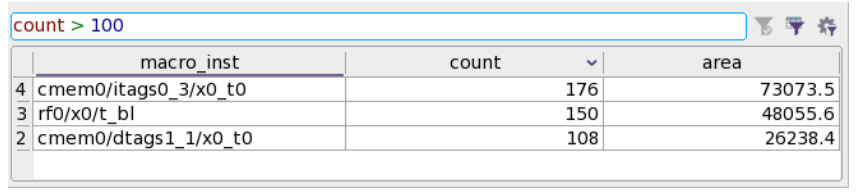
\includegraphics[width=0.92\textwidth]{gui-fig-146.png}
\caption{过滤绘图数据}
\label{fig:gui-146}
\end{figure}

\subsection{定制绘图}
\subsubsection*{Customizing a Plot}

可以修改绘图，以便：
\begin{itemize}
  \item 用 \textbf{View Settings > Properties} 或 \cmd{gui\_set\_charts\_property} 命令定制外观
  \item 用 \textbf{View Settings > Annotations} 或 \cmd{gui\_create\_charts\_*\_annotation} 命令添加标注
  \item 用 \textbf{View Settings > Plots}，或 \cmd{gui\_place\_charts\_plots} 与 \cmd{gui\_group\_charts\_plots} 命令，在视图中排布多个绘图
  \item 用 \cmd{gui\_connect\_charts\_signal} 命令，在用户交互时运行自定义 Tcl 过程
\end{itemize}

% 第 13 章 Using the PG Pattern Viewer
\bichapter{使用 PG Pattern 查看器}{Using the PG Pattern Viewer}
\label{chap:gui-pg}

IC Compiler II GUI 提供 PG Pattern 窗口，用于创建并预览电源地图案（PG pattern）。用该窗口查看一组预置的 PG pattern 模板（template）。为某个 PG pattern 选定模板之后，把图案模板复制到 PG Pattern Editor，并编辑图案，使之符合设计要求。若图案使用参数（parameter），可以在 PG Pattern 窗口中设置参数。预览图案，并对 Tcl 命令做必要的修改。只有在图案定稿之后，才回到版图窗口，把图案实例化到设计中。

关于 PG Pattern 窗口的更多信息，见下列主题：
\begin{itemize}
  \item 选择 PG Pattern 模板
  \item 预览模板 PG Pattern
  \item 预览已有的图案与策略定义
  \item 高亮单个图案
\end{itemize}

PG Pattern 窗口见图~\ref{fig:gui-147}。

\begin{figure}[htbp]
\centering
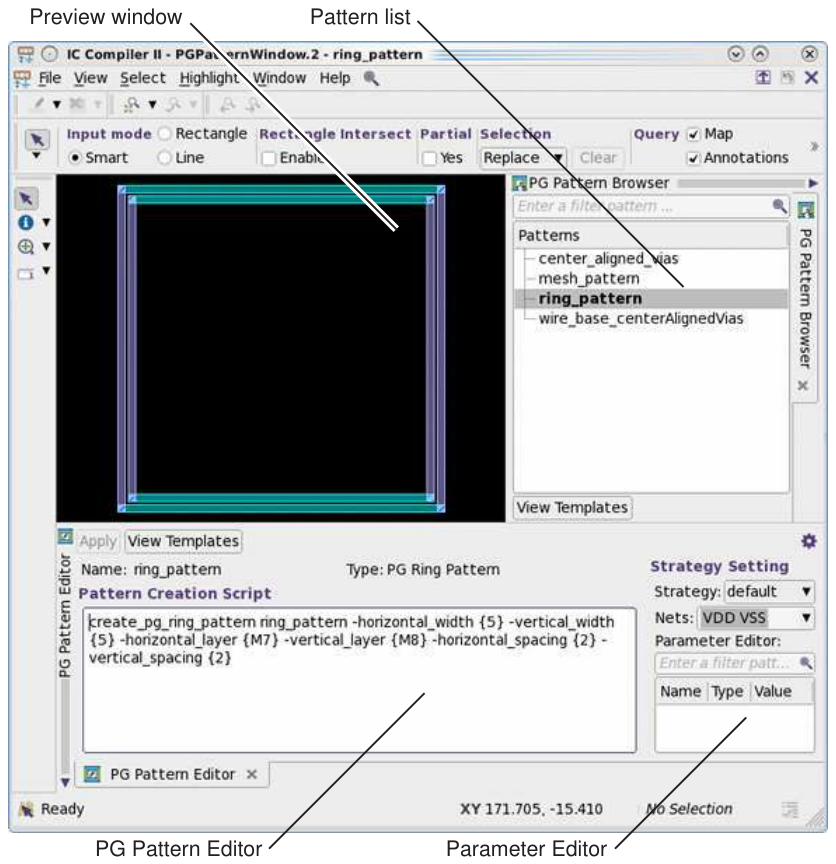
\includegraphics[width=0.92\textwidth]{gui-fig-147.png}
\caption{PG Pattern 窗口}
\label{fig:gui-147}
\end{figure}

图中引出线标出：预览窗口（Preview window）、图案列表（Pattern list）、PG Pattern Editor、Parameter Editor。

\section{选择 PG Pattern 模板}
\subsection*{Selecting a PG Pattern Template}

PG Pattern 窗口包含一组预置模板，可作为创建自己图案的起点。从菜单选择 \textbf{Window > PG Pattern Window}，打开 PG Pattern 窗口。要在 PG Pattern 窗口中查看并选择模板：
\begin{enumerate}
  \item 在 PG Pattern 窗口中单击 View Templates 按钮，打开 PG templates 对话框。
  \item （可选）在 PG Pattern Templates 对话框的过滤模式框中输入字符串，以过滤模板列表。匹配不区分大小写。例如，输入“Mesh”或“mesh”，只显示名称中包含单词 Mesh 的模板。
  \item 在列表中单击模板名以选择模板。工具在 PG Pattern Template 窗口中显示该模板。典型模板包含简短说明、图案图像，以及用于创建该图案的 Tcl 命令。
  \item 单击 Send to Editor 按钮，把模板复制到 PG Pattern 窗口中的 PG Pattern Editor。
\end{enumerate}

\begin{figure}[htbp]
\centering
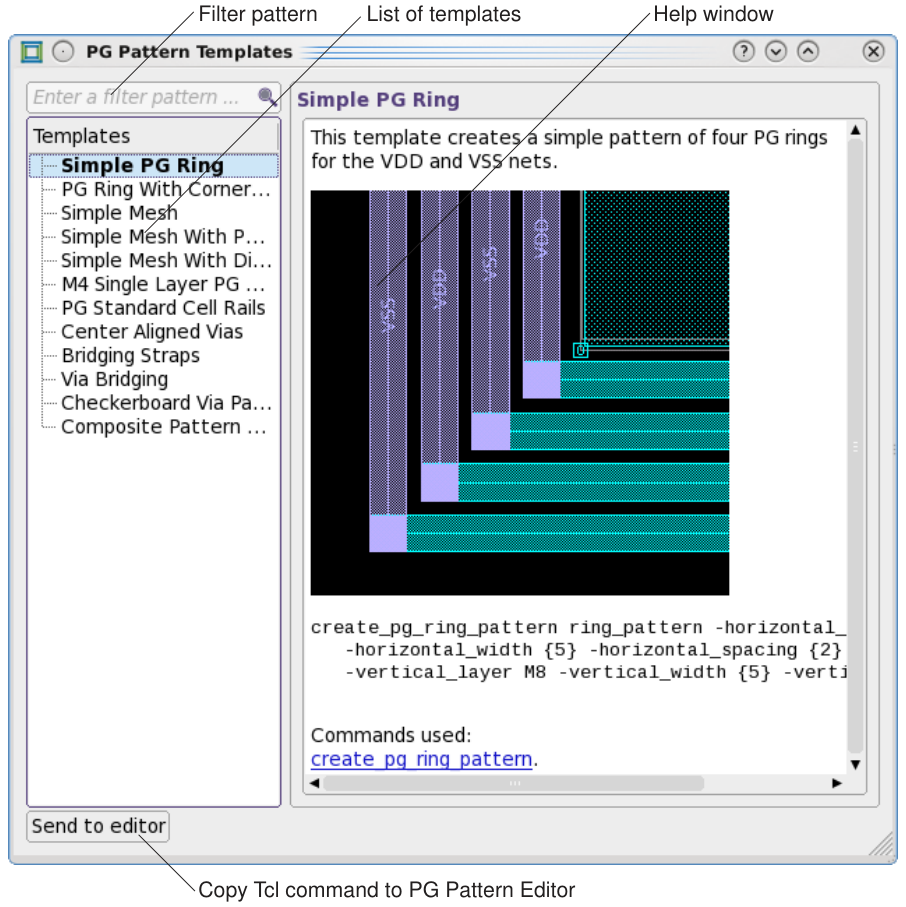
\includegraphics[width=0.92\textwidth]{gui-fig-148.png}
\caption{PG Pattern 模板}
\label{fig:gui-148}
\end{figure}

图中引出线标出：过滤模式（Filter pattern）、模板列表（List of templates）、帮助窗口（Help window），以及把 Tcl 命令复制到 PG Pattern Editor（Copy Tcl command to PG Pattern Editor）。

\section{预览模板 PG Pattern}
\subsection*{Previewing a Template PG Pattern}

图案预览功能在预览窗口中显示模板图案。使用图案预览功能：
\begin{enumerate}
  \item 按“选择 PG Pattern 模板”中所述，把图案模板复制到 PG Pattern Editor。
  \item （可选）修改图案的层、间距、宽度及其他参数，使之与当前设计一致。
  \item 单击 Apply 按钮，在预览窗口中显示图案。
\end{enumerate}

工具会运行 PG Pattern Editor 面板中指定的 \cmd{create\_*\_pattern} 命令，并把图案名加入 PG Pattern Browser 的图案列表。在版图窗口中使用 \cmd{report\_pg\_patterns} 命令，可为设计中当前已定义的图案写出详细报告。创建图案时若出现错误，工具把错误信息写到控制台（console）。

\section{预览已有的图案与策略定义}
\subsection*{Previewing Existing Pattern and Strategy Definitions}

可以用 PG Pattern 窗口按下列步骤预览先前定义的图案和策略：
\begin{enumerate}
  \item 在版图窗口中运行 \cmd{create\_pg\_ring\_pattern}、\cmd{create\_pg\_ring\_pattern} 或其他创建图案的命令，以创建 PG pattern。可以在打开 PG Pattern 窗口之前或之后创建图案。在版图窗口中定义的任何 PG pattern，都会列在 PG Pattern Browser 下的 Patterns 列表中。本例定义了四个环形图案（ring pattern）。

\begin{figure}[htbp]
\centering
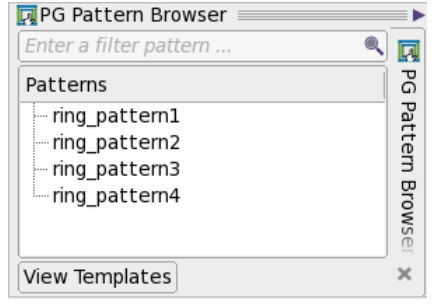
\includegraphics[width=0.92\textwidth]{gui-fig-149.png}
\caption{预定义图案}
\label{fig:gui-149}
\end{figure}

  \item （可选）单击鼠标右键，并从上下文菜单中选择 Delete，以从列表中删除某个图案。

\begin{figure}[htbp]
\centering
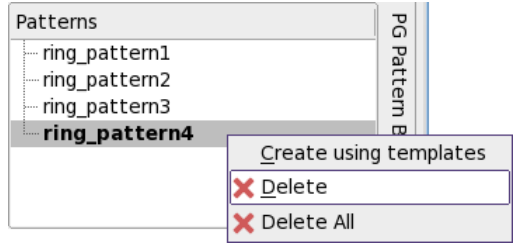
\includegraphics[width=0.92\textwidth]{gui-fig-150.png}
\caption{图案列表的上下文菜单}
\label{fig:gui-150}
\end{figure}

  \item 在列表中单击某个图案以选中它，并在 Pattern Creation Script 编辑器中显示对应的 \cmd{create\_*\_pattern} 命令。
  \item （可选）在编辑器中修改图案。
  \item （可选）用 \cmd{set\_pg\_strategy} 命令创建一个或多个 PG 策略（PG strategy）。
  \item （可选）在 Strategy Setting 下的 Strategy 框中，选择用于创建图案的策略。Strategy 框中只显示所选图案可用的策略。工具也会为所选图案创建一个默认策略。
  \item 单击 Apply，按所选策略和图案在预览窗口中创建图案。

\begin{noteBox}
图案只创建在预览窗口中，不会创建到当前设计的版图窗口里。
\end{noteBox}

  \item （可选）从图案列表中另选一个图案，或从策略框中另选一个策略，并重复上一步，以生成新图案。
\end{enumerate}

\section{高亮单个图案}
\subsection*{Highlighting Individual Patterns}

PG Pattern 查看器支持在一个图案内部高亮各个子图案（child pattern）。用该功能高亮某个图案定义里子图案的电源条带（power strap）和通孔（via），并调整金属层（metal layer）、层宽、间距等。要查看图案中的单个子图案：
\begin{enumerate}
  \item 从图案模板列表中选择图案，例如通孔桥接图案（via bridging pattern）。
  \item 单击鼠标右键，并从列表中选择子图案编号。工具会高亮组成该图案编号的金属形状。
\end{enumerate}

下图为示例 via bridging 复合图案（composite pattern），其中第二个图案被高亮。

\begin{figure}[htbp]
\centering
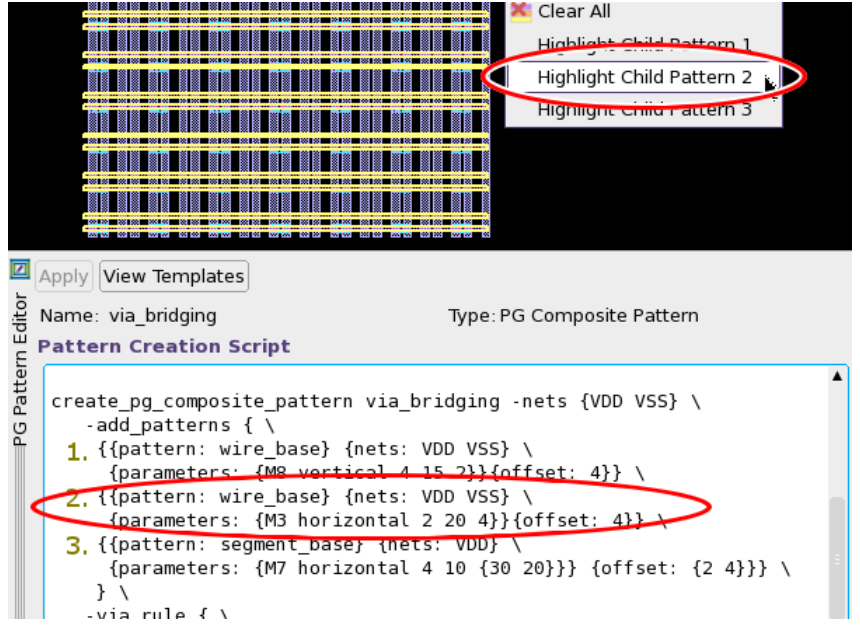
\includegraphics[width=0.92\textwidth]{gui-fig-151.png}
\caption{高亮子图案}
\label{fig:gui-151}
\end{figure}

% 第 14 章 Creating Routes
\bichapter{创建布线}{Creating Routes}
\label{chap:gui-route}

IC Compiler II GUI 提供交互界面与程序化接口，用来快速创建布线（route）。使用 Create Route 工具，可在设计中的管脚（pin）、端口（port）以及其他布线形状（route shape）之间，为一根或多根线网（net）或线束（bundle）布线。与 Create Route 工具类似，Create RDL 工具用于为单根线网布线，在再分布层（redistribution layer，RDL）或其他金属层上创建正交布线与 45 度布线。\cmd{create\_trunk}、\cmd{create\_trunk\_pin\_to\_pin} 与 \cmd{create\_trunk\_pin\_to\_trunk} 命令根据命令行选项，在指定线网上创建布线段。

下列主题说明如何使用 GUI 创建布线：
\begin{itemize}
  \item 交互创建布线
  \item 对布线做交互式设计规则检查
  \item 用 Tcl 命令或 GUI 创建布线主干
  \item 在布线上添加缓冲器
  \item 估算点到点电阻
\end{itemize}

% ============================================================
\section{交互创建布线}
\subsection*{Creating Routes Interactively}

Create Route 工具可以交互地为一根或多根线网或线束布线。工具选项指定布线的创建方式。工具支持避开阻挡（blockage），并提供设计规则检查（design rule checking，DRC）反馈，帮助创建高质量、无违例（violation）的布线与连接。吸附（snapping）、自动对齐（auto-alignment）与自动焊接（auto-welding）用于把新布线快速接到管脚或已有布线上。线束布线（bundle routing）支持同时为多条信号布线。

\subsection{启动 Create Route 工具}
\subsubsection*{Starting the Create Route Tool}

要启动 Create Route 工具，采用下列任一方式：
\begin{itemize}
  \item 单击 Create Route 按钮
  \item 在菜单中选择 \textbf{Create > Route}
  \item 按 Shift+R
\end{itemize}

工具启动并显示 Create Route 工具栏。

\subsection{指定层、线宽、节距与端帽样式}
\subsubsection*{Specifying Layer, Width, Pitch, and End-Cap Style}

Create Route 工具在工具栏上提供设置与选项，用来指定布线的层、线宽、节距（pitch）与端帽样式（end-cap style），如图~\ref{fig:gui-152} 所示。单击工具栏上的 More、DRC 或 Snap 按钮，还可以使用其他设置。

\begin{figure}[htbp]
\centering
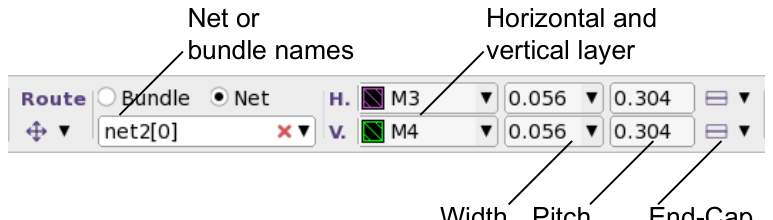
\includegraphics[width=0.92\textwidth]{gui-fig-152.png}
\caption{层名、线宽、节距与端帽设置}
\label{fig:gui-152}
\end{figure}

可用下列任一方法指定线网或线束的层名、线宽与节距：
\begin{itemize}
  \item 在输入框中输入线网名或线束名。工具把水平层与垂直层设为用于布线的最低金属层。
  \item 在启动 Create Route 工具之前选择一个管脚，以便推断线网名。工具根据所选管脚设置层、线宽等参数。
  \item 在工具栏 Auto 部分选择 Net，然后单击一条已有布线，从该布线推断线网名。若要从已有布线推断层、线宽或端帽样式，在 Auto 部分选择对应选项。
  \item 在工具栏的 More 设置面板中启用 Connect to pin by layer，并指定层名。自动连接到管脚时，工具使用指定的层，除非这些管脚是布线的起点或终点。
\end{itemize}

\subsection{在管脚之间创建布线}
\subsubsection*{Creating Routes Between Pins}

为一组管脚创建布线：
\begin{enumerate}
  \item 选择要布线的线网的源管脚或目标管脚。
  \item 按 Shift+R，或单击 Create Route 工具按钮，启动 Create Route 工具。
  \item 在工具栏单击 More，并在 Advanced options 部分选择 Extend first 与 Extend last。
\end{enumerate}

\begin{figure}[htbp]
\centering
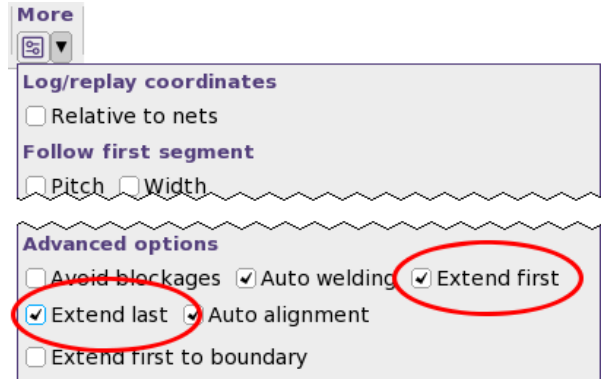
\includegraphics[width=0.92\textwidth]{gui-fig-153.png}
\caption{管脚到管脚连接布线的设置}
\label{fig:gui-153}
\end{figure}

\begin{enumerate}
  \setcounter{enumi}{3}
  \item 把指针放在靠近所选管脚的布线路径上并单击鼠标，开始绘制布线，如图~\ref{fig:gui-154} 中的（A）所示。
\end{enumerate}

\begin{figure}[htbp]
\centering
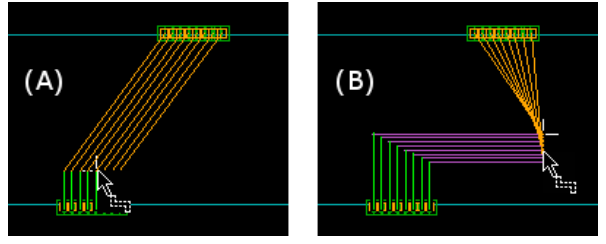
\includegraphics[width=0.92\textwidth]{gui-fig-154.png}
\caption{从所选管脚布线}
\label{fig:gui-154}
\end{figure}

\begin{enumerate}
  \setcounter{enumi}{4}
  \item 单击以创建一个拐角，然后沿正交方向移动鼠标指针，如图中的（B）所示。按需要重复本步，以创建更多布线段。
  \item 把鼠标指针移到目标管脚附近，直到工具显示完成的布线，如图~\ref{fig:gui-155} 中的（C）所示。
\end{enumerate}

\begin{figure}[htbp]
\centering
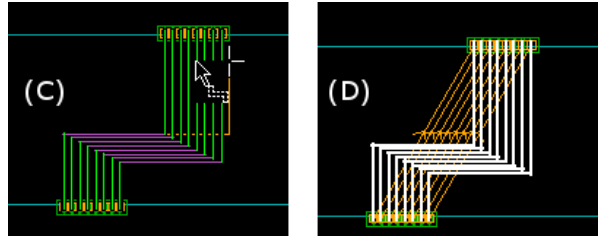
\includegraphics[width=0.92\textwidth]{gui-fig-155.png}
\caption{完成布线}
\label{fig:gui-155}
\end{figure}

\begin{enumerate}
  \setcounter{enumi}{6}
  \item 按 Enter 键，或单击鼠标右键并在上下文菜单中选择 Apply，完成布线。工具完成的布线如图中的（D）所示。
\end{enumerate}

\subsection{按第一段套用布线段的线宽与间距}
\subsubsection*{Applying Route Segment Width and Spacing Based on the First Segment}

要使全部布线段采用与第一段相同的线宽与间距，在工具栏单击 More，并在 Follow first segment 部分启用 Pitch 与 Width。启用后，工具使后续全部布线段与第一段一致，如图~\ref{fig:gui-156} 所示。

\begin{figure}[htbp]
\centering
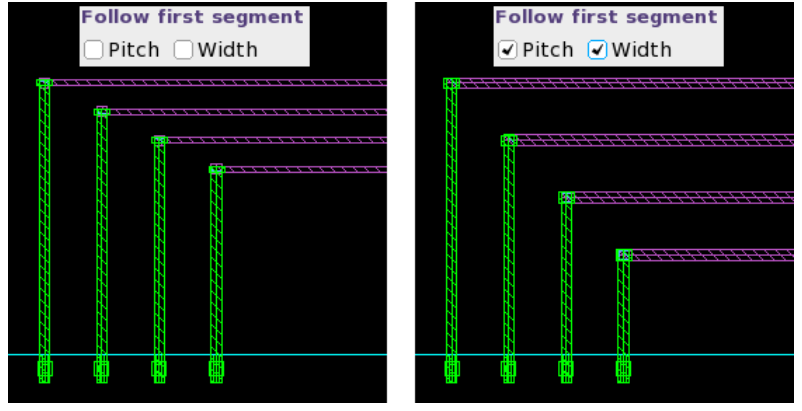
\includegraphics[width=0.92\textwidth]{gui-fig-156.png}
\caption{跟随第一段}
\label{fig:gui-156}
\end{figure}

\subsection{创建偏离轨道的布线}
\subsubsection*{Creating Off-Track Routes}

要创建偏离轨道（off-track）的布线段，在工具栏单击 More，并在 Snap to track 部分关闭 First net 与 Every net。默认启用 First net，第一段布线创建在布线轨道（track）上。这些选项如图~\ref{fig:gui-157} 所示。

\begin{figure}[htbp]
\centering
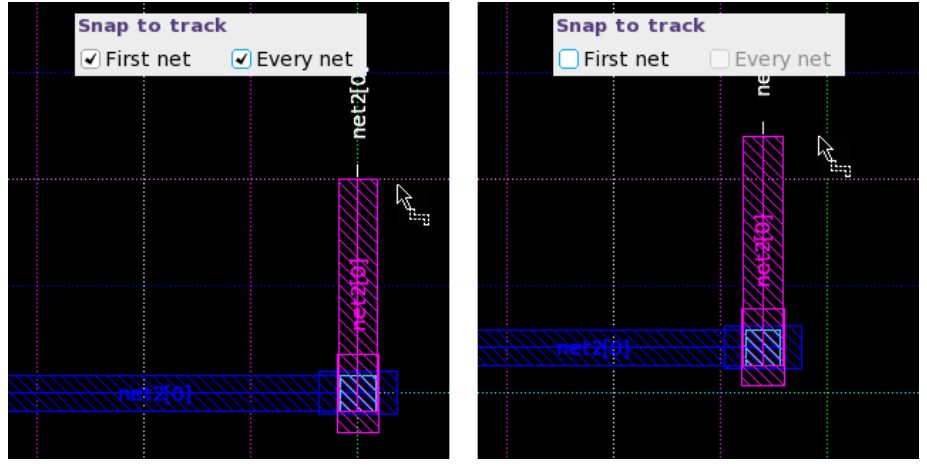
\includegraphics[width=0.92\textwidth]{gui-fig-157.png}
\caption{吸附到轨道}
\label{fig:gui-157}
\end{figure}

\subsection{在所绘路径的上方或下方创建后续布线}
\subsubsection*{Creating Successive Routes Above or Below the Drawn Path}

Create Route 工具从线束或线网名输入框中的第一根线网开始，沿用鼠标绘制的路径创建布线。后续线网与第一根线网平行创建；方向由 More 设置面板中 When starting use 部分的 Low end 与 High end 决定。

下面的示例用 \cmd{create\_bundle} 命令创建名为 \cmd{bundle4} 的线束，并用它为四根线网布线：
\begin{lstlisting}
icc2_shell> create_bundle -name {bundle4} \
    {net2[127] net2[126] net2[125] net2[124]}
\end{lstlisting}

列表中的第一根线网是 \cmd{net2[127]}，它沿用鼠标绘制的路径创建。默认情况下，后续线网创建在 \cmd{net2[127]} 的上方或右侧，如图~\ref{fig:gui-158} 左侧所示。黄色高亮表示用鼠标绘制布线时的路径。

\begin{figure}[htbp]
\centering
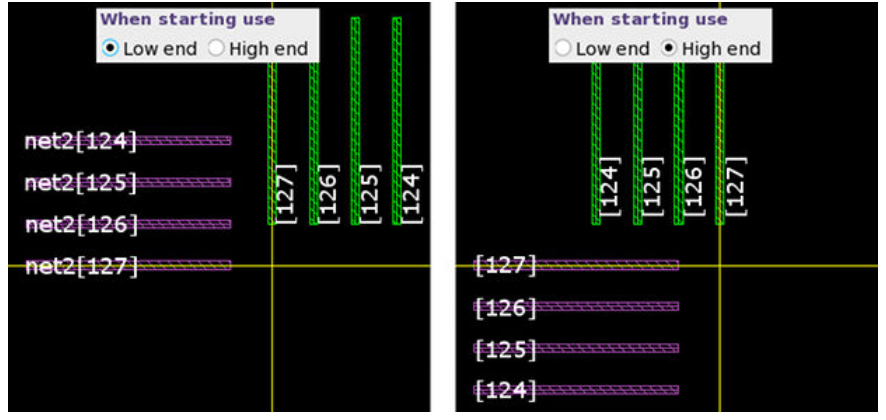
\includegraphics[width=0.92\textwidth]{gui-fig-158.png}
\caption{低端与高端布线选项}
\label{fig:gui-158}
\end{figure}

要使后续布线位于鼠标路径的下方或左侧，在工具栏单击 More 并选择 High end。工具创建的布线如图~\ref{fig:gui-158} 右侧所示。

\subsection{更改正交布线的线网顺序}
\subsubsection*{Changing the Route Ordering for Orthogonal Routes}

创建正交布线时，Create Route 工具支持多种线网排序方式。默认情况下，工具保持线网顺序，并在创建新布线段时避免布线重叠。要在创建正交布线时反转布线顺序，单击 More，并在 When turning 部分启用 Switch ends。要在拐弯处把布线错开，启用 Switch ends，并把 Skip count 设为大于 1 的值。设置这些选项后的布线结果如图~\ref{fig:gui-159} 所示。

\begin{figure}[htbp]
\centering
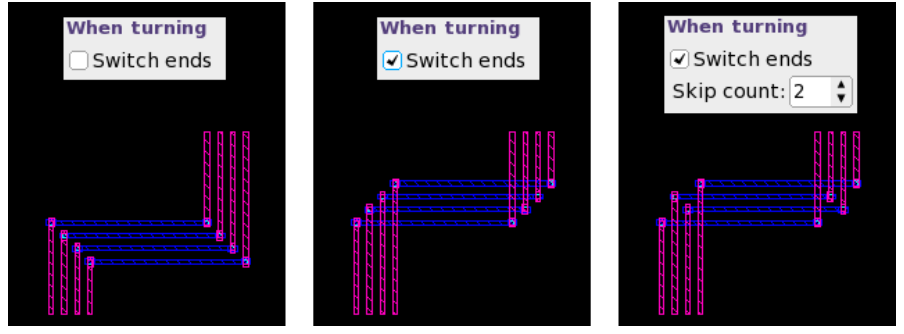
\includegraphics[width=0.92\textwidth]{gui-fig-159.png}
\caption{布线拐弯样式}
\label{fig:gui-159}
\end{figure}

\subsection{显示布线引导飞线与标注}
\subsubsection*{Displaying Route Guidance Flylines and Annotations}

Create Route 工具显示飞线（flyline）与其他引导，帮助创建布线。启动 Create Route 工具并输入线网名后，工具在布线的管脚与端口之间显示一条静态飞线（static flyline）。开始布线后，工具再加入一条动态飞线（dynamic flyline），显示到最近管脚连接的最短路径；移动鼠标创建布线段时，动态飞线随之更新。布线完成后，动态飞线被去掉。默认情况下，工具在布线的管脚与端口之间显示飞线，并在布线中的端口上显示端口引导标记（port guidance marker）。

要隐藏飞线与端口引导标记，单击 More，并在面板 Show 部分取消选择 Port Guidance 与 Flylines。要显示已有布线，以及随布线段创建而动态更新的当前布线电阻值，在面板中选择 Routes 与 Resistance。面板中的选项以及与这些选项对应的版图标注如图~\ref{fig:gui-160} 所示。

\begin{figure}[htbp]
\centering
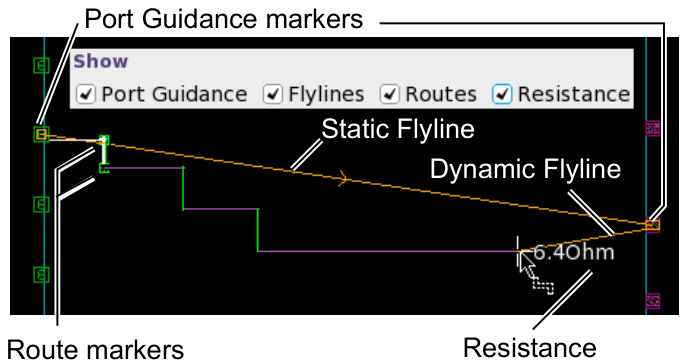
\includegraphics[width=0.92\textwidth]{gui-fig-160.png}
\caption{显示飞线与其他标注}
\label{fig:gui-160}
\end{figure}

\subsection{避免连接到已有布线}
\subsubsection*{Preventing Connections to Existing Routes}

要避免工具在跨越同一线网的布线时自动创建通孔（via），单击 More，并在面板 Advanced options 部分取消选择 Auto welding。更改该选项后的布线结果如图~\ref{fig:gui-161} 所示。

\begin{figure}[htbp]
\centering
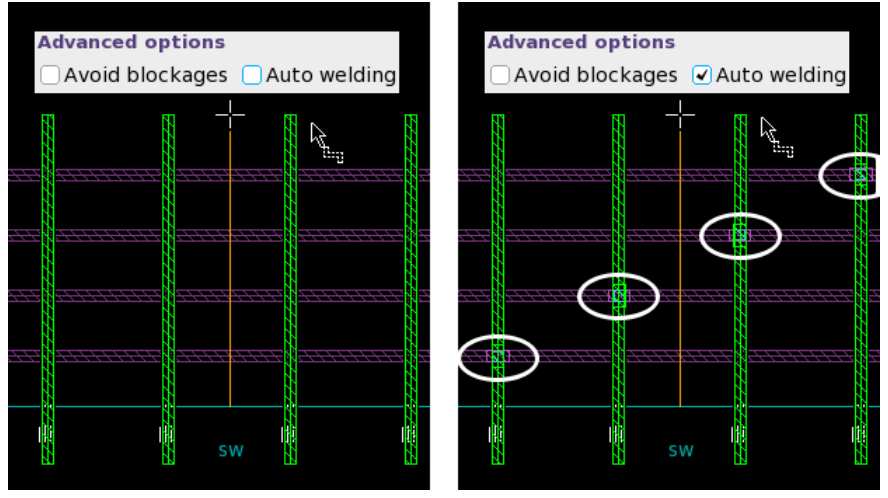
\includegraphics[width=0.92\textwidth]{gui-fig-161.png}
\caption{自动焊接}
\label{fig:gui-161}
\end{figure}

\subsection{设置搜索距离并指定搜索层}
\subsubsection*{Setting a Search Distance and Specifying Layers to Search}

Create Route 工具会自动连接到位于当前鼠标位置搜索距离（search distance）之内的管脚。若已启用 Auto welding，而又不希望工具连接到管脚，单击 More，并把 Welding and extend options 部分中 Search distance 框的值设为 0。若希望工具连接到更远的管脚，增大该距离，使工具能搜索离布线更远的管脚。同一组管脚、沿黄色高亮绘制的同一条布线，在不同搜索距离下的版图结果如图~\ref{fig:gui-162} 所示。

\begin{figure}[htbp]
\centering
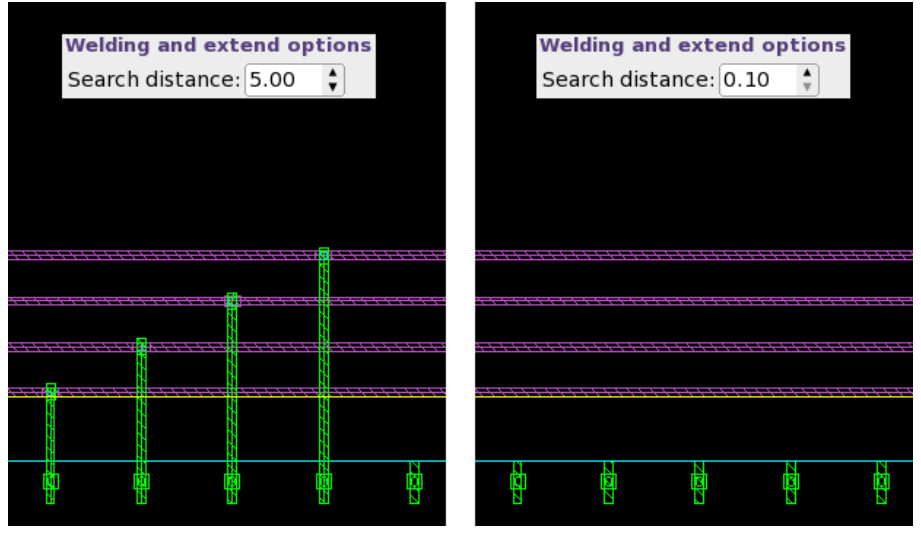
\includegraphics[width=0.92\textwidth]{gui-fig-162.png}
\caption{搜索距离}
\label{fig:gui-162}
\end{figure}

工具在全部布线层上搜索连接。要把搜索限制在相邻层，单击 More，并在面板 Welding and extend options 部分选择 Search Layers: Adjacent。选中后，工具只连接到与当前布线层相邻的一层上的管脚。要指定搜索的层范围，在同一部分选择 Specified，并在层列表框中选择一层或多层。

\subsection{指定其他焊接与连接选项}
\subsubsection*{Specifying Other Welding and Connection Options}

Create Route 工具还提供其他选项，用来指定与已有布线或管脚的连接。
\begin{itemize}
  \item \textbf{Ignore pin access direction}：选中后，工具自动把布线连接到管脚，不考虑管脚接入方向（pin access direction）。默认会考虑管脚接入方向。
  \item \textbf{Skip PG nets}：选中后，避免连接到电源地（power and ground，PG）线网。当这些线网用于线网屏蔽（net shielding）时，用本选项跳过与地线网的连接。
  \item \textbf{Honor via to via spacing}：选中后，工具遵守同一线网的通孔到通孔间距（via-to-via spacing）规则。
  \item \textbf{No via on pin}：连接到管脚时避免插入通孔。
  \item \textbf{Adjust to pin width}：选中后，若线宽小于管脚宽度，工具把布线宽度设为管脚宽度。默认不选中本选项，线宽在工具栏中指定。若线宽大于管脚宽度，则采用管脚宽度作为线宽。
  \item \textbf{Align with pin center}：取消选择后，工具把连接线与最近的平行管脚边对齐，或把线延伸到平行管脚边的边界之内。轨道吸附与间距要求可能影响最终的线位置。默认选中本选项，工具在可能时把布线与管脚包围盒（bounding box）的中心对齐。当管脚宽于连接线时，工具可能把线移离中心，以遵守轨道吸附与间距设置。
\end{itemize}

\subsection{创建 45 度布线与 RDL 布线}
\subsubsection*{Creating 45-Degree and RDL Routes}

Create RDL 工具支持 Create Route 工具的许多相同功能。此外，Create RDL 工具可以在再分布层上创建 RDL 布线，并在单一金属层上创建一般的 45 度布线，如图~\ref{fig:gui-163} 所示。

\begin{figure}[htbp]
\centering
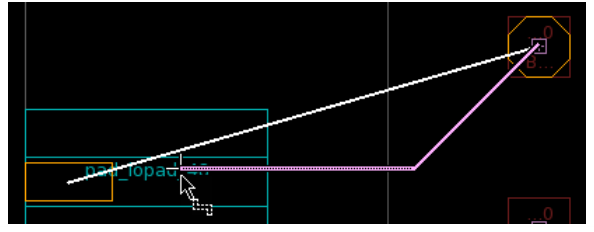
\includegraphics[width=0.92\textwidth]{gui-fig-163.png}
\caption{Create RDL 工具}
\label{fig:gui-163}
\end{figure}

用 Create RDL 工具创建 45 度布线：
\begin{enumerate}
  \item 在菜单中选择 \textbf{Create > RDL}，或单击 Create RDL 按钮，启动 Create RDL 工具。
  \item 在线网名输入框中输入要布线的线网或线束名。
  \item （可选）单击 More，并在 More options 面板中修改设置。Create RDL 工具支持许多与 Create Route 工具相同的设置，例如前面各节所述的 extend first、extend last、high end、low end 等。
  \item 单击工具栏左侧的 Route 按钮，并选择布线该线网所用的角度。该设置决定布线的创建方式，如图~\ref{fig:gui-164} 所示。
\end{enumerate}

\begin{figure}[htbp]
\centering
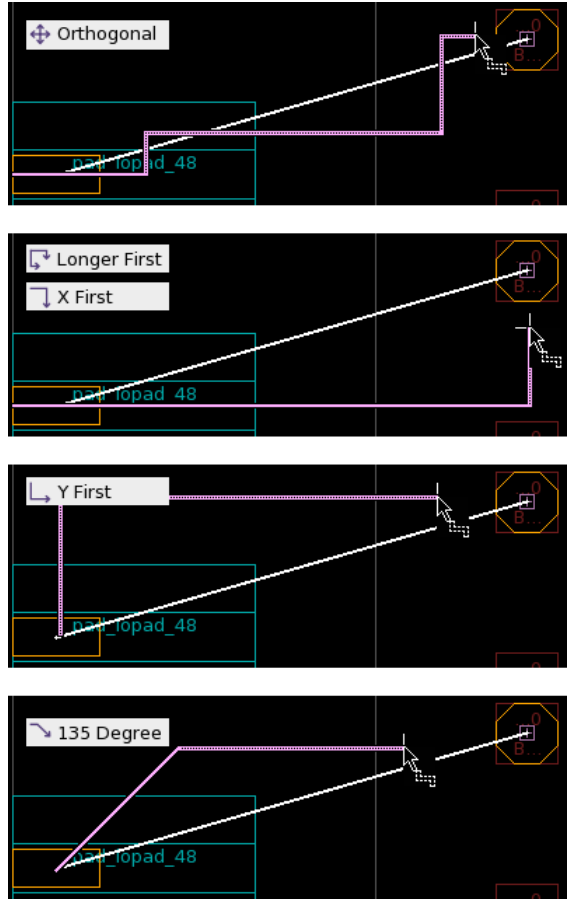
\includegraphics[width=0.92\textwidth]{gui-fig-164.png}
\caption{Create RDL 绘制模式}
\label{fig:gui-164}
\end{figure}

\begin{enumerate}
  \setcounter{enumi}{4}
  \item 单击管脚、端口或线网连接，开始布线。
  \item 单击以完成一段布线，并开始新的一段。
  \item 按 Enter 完成布线。
\end{enumerate}

\subsection{录制并回放 Create Route 操作}
\subsubsection*{Recording and Replaying Create Route Actions}

Create Route 与 Create RDL 工具支持录制功能，用来捕获创建布线时的鼠标操作，并保存到 Script Editor。脚本可以存到磁盘，以后再运行；也可以直接从 Script Editor 运行。录制功能可以配置为容忍管脚位置的小幅变化，从而在设计做过小改动之后重新创建布线。

要创建布线并启用录制：
\begin{enumerate}
  \item 选择 \textbf{Create > Route}、单击 Create Route 按钮，或按 Shift+R，启动 Create Route 工具。选择 \textbf{Create > RDL}，或单击 Create RDL 按钮，启动 Create RDL 工具。
  \item （可选）在工具栏中设置所需的布线选项。
  \item （可选）若预计重新创建布线时，布线中的管脚或线段坐标会发生变化，单击 More，并在 Log/replay coordinates 部分启用 Relative to nets。启用后，工具捕获的是相对整条布线包围盒的坐标，而不是绝对坐标。若要把脚本用于在设计的另一区域创建布线，本选项很有用。
  \item 在 Create Route 工具的工具栏上单击 Record 按钮。
  \item 单击起点、创建线段并结束布线，从而创建该布线。
  \item 布线完成后，打开 Script Editor，单击 Save As 按钮，把脚本保存到文件。
\end{enumerate}

创建线段时，Create Route 工具把操作捕获到 Script Editor。录制功能捕获的示例脚本如下：
\begin{lstlisting}
...
# Info : recording session started
...
gui_mouse_tool -window [gui_get_current_window -types Layout -mru] \
   -start CreateRouteTool
set_edit_setting -default
set_snap_setting -default
...
gui_set_mouse_tool_option -tool CreateRouteTool -all -default
gui_set_mouse_tool_option -tool CreateRouteTool \
   -option {BundleOrNetNames} \
   -value {net2[127] net2[126] net2[125] net2[124]}
...
gui_mouse_tool -window [gui_get_current_window -types Layout -mru] \
   -add_point {455.756 907.825} -scale 0.02
gui_mouse_tool -window [gui_get_current_window -types Layout -mru] \
   -add_point {568.946 1194.223} -scale 5.6331
...
gui_mouse_tool -window [gui_get_current_window -types Layout -mru] -apply
gui_mouse_tool -window [gui_get_current_window -types Layout -mru] -abort
...
# Info : recording session ended
\end{lstlisting}

要重新创建该布线，在 Script Editor 中单击 Run Script 运行脚本。也可以把脚本保存到文件，再用 \cmd{source} 命令执行该脚本。

% ============================================================
\section{对布线做交互式设计规则检查}
\subsection*{Performing Interactive Design Rule Checking on Routes}
\label{sec:gui-route-drc}

GUI 提供两种交互式设计规则检查：
\begin{itemize}
  \item Editor DRC
  \item ICV Live
\end{itemize}

\begin{seeAlsoBox}
Editor DRC 工具的进一步说明，见第~\ref{sec:gui-editor-drc}~节「用 Editor DRC 工具诊断设计规则违例」。ICV Live 功能见 \textit{IC Compiler II Implementation User Guide} 中的 Checking Signoff Design Rules Interactively in the GUI。
\end{seeAlsoBox}

\subsection{用 Editor DRC 工具诊断设计规则违例}
\subsubsection*{Diagnosing Design Rule Violations Using the Editor DRC tool}
\label{sec:gui-editor-drc}

版图视图（layout view）提供 Editor DRC 工具，用来识别并诊断交互编辑操作引起的 DRC 违例。Editor DRC 工具检测设计规则违例，在当前版图视图中显示错误形状，并把违例记入 Editor DRC 错误数据文件。

\begin{noteBox}
Editor DRC 工具只做快速检查，并按工艺文件（technology file）中定义的一组 DRC 规则显示错误。Editor DRC 工具不能代替 IC Validator 这类完整的 DRC 工具。
\end{noteBox}

除 Create Route 工具外，下列版图编辑工具也与 Editor DRC 工具配合使用：
\begin{itemize}
  \item Copy Objects 工具
  \item Create Fill 工具
  \item Create RDL 工具
  \item Create Shape 工具
  \item Create Terminal 工具
  \item Create Via 工具
  \item Quick Connect 工具
  \item Stretch Connected 工具
  \item Stretch 工具
\end{itemize}

\subsection{交互验证布线编辑}
\subsubsection*{Verifying Route Edits Interactively}

要为交互编辑操作启用或关闭 Editor DRC 工具，单击工具栏上的 DRC 按钮，并选择 DRC enabled。

为交互编辑操作启用 Editor DRC 工具后，若检测到违例，工具立即给出可视反馈。版图视图为每种违例显示不同的视觉提示。

Editor DRC 工具支持对下列类型的对象做规则检查：
\begin{itemize}
  \item 水平与垂直的线网形状和用户形状（user shape），包括线、通孔、通孔阵列（via array）、路径（path）、多边形（polygon）与矩形（rectangle）
  \item 端口形状与端子（terminal）
  \item 标准单元（standard cell）、硬宏（hard macro）、软宏（soft macro）与黑盒（black box）
  \item 布线阻挡（routing blockage）
\end{itemize}

\subsection{验证已编辑的线网}
\subsubsection*{Verifying Edited Nets}

要检查所选线网是否存在 Editor DRC 工具违例：
\begin{enumerate}
  \item 选择需要检查的一根或多根线网。
  \item 选择 \textbf{Edit > DRC > Run DRC on Selected Shapes}。也可以使用 \cmd{gui\_check\_drc\_errors} 命令。
\end{enumerate}

若发现错误，工具创建错误数据，并打开 Error Browser 显示这些错误数据。

\subsection{设置 Editor DRC 选项}
\subsubsection*{Setting Editor DRC Options}

Editor DRC 工具按工艺文件中定义的一组 DRC 规则做规则检查。交互编辑工具使用 Editor DRC 工具，检测交互编辑期间出现的布线设计规则违例。可以设置工具能够检测的最大违例数，并控制检测到违例时工具是否自动打开错误浏览器并加载错误。

当支持 Editor DRC 的工具处于活动状态时，单击工具栏上的 DRC 按钮，即可设置 Editor DRC 工具选项。

在 Editor DRC options 对话框中更改选项后，更改立即作用于全部已打开版图视图中所有适用的工具。若在 Application Preferences 对话框中启用了 GUI 命令输出日志，工具还会在控制台（console）日志视图与历史视图中显示 \cmd{set\_edrc\_setting} 命令，从而记录这次更改。

\subsection{查看 Editor DRC 报告的错误}
\subsubsection*{Examining Errors Reported by Editor DRC}

Editor DRC 工具检测到设计规则违例时，在当前版图视图中显示错误形状，把错误记入 Editor DRC 错误视图，并自动把错误信息加载到错误浏览器，如图~\ref{fig:gui-165} 所示。

\begin{figure}[htbp]
\centering
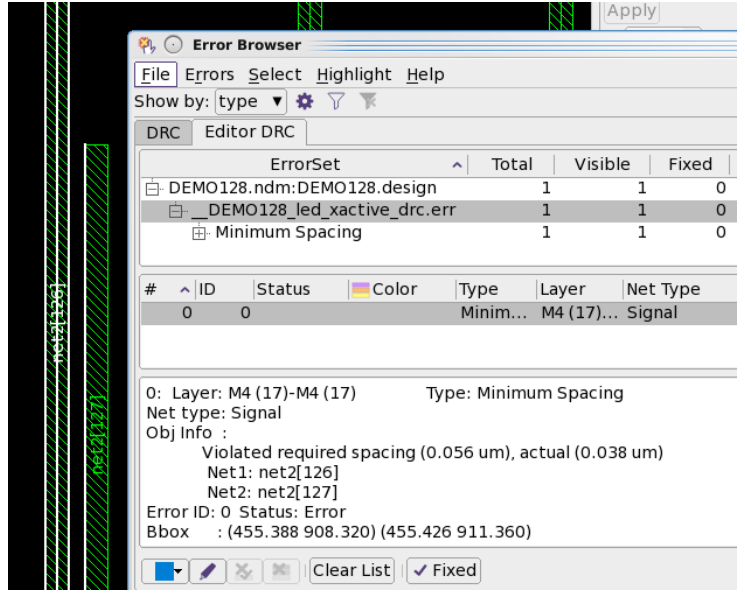
\includegraphics[width=0.92\textwidth]{gui-fig-165.png}
\caption{Editor DRC}
\label{fig:gui-165}
\end{figure}

错误视图包含两类违例记录：交互编辑期间检测到的违例，以及对所选形状运行检查时检测到的违例。修正违例、撤销引起违例的编辑操作、关闭用于检测该违例的设计规则检查，或在错误浏览器中删除错误时，Editor DRC 工具会更新错误数据。

Editor DRC 错误视图与当前设计关联。在关闭设计或更改当前设计之前，它一直打开并加载在错误浏览器中。保存或关闭设计时，工具不保存该错误视图。若关闭当前设计，Editor DRC 工具会关闭错误视图，并从错误浏览器中去掉这些错误。

% ============================================================
\section{用 Tcl 命令或 GUI 创建布线主干}
\subsection*{Creating Route Trunks With Tcl Commands or GUI}

IC Compiler II GUI 支持用 Tcl 命令为指定线网和线束创建布线主干（route trunk）。使用 \cmd{create\_trunk}、\cmd{create\_trunk\_shared\_track}、\cmd{create\_trunk\_pin\_to\_trunk}、\cmd{create\_trunk\_pin\_to\_pin} 与 \cmd{create\_trunk\_topology} 命令创建主干线段与连接，如本节所述。

\subsection{沿一个方向创建布线段}
\subsubsection*{Creating Route Segments in One Direction}

要在单一金属层上沿一个方向创建布线主干，按如下方式使用 \cmd{create\_trunk} 命令：
\begin{lstlisting}
icc2_shell> set nets [get_nets {net1 net2 net3 net4}]
icc2_shell> create_trunk -nets $nets -layer M3 \
   -gravity percentage -percentage 25
\end{lstlisting}

该命令为 \opt{-nets} 选项指定的每根线网或每个线束创建一条布线段。本例中，\opt{-gravity percentage} 指定布线段如何与这些线网的包围盒对齐。\opt{-percentage 25} 指定第一条布线段放在包围盒底边再加上包围盒高度 25\% 的位置。百分比取 25、50 与 75 时的不同布线结果如图~\ref{fig:gui-166} 所示。

\begin{figure}[htbp]
\centering
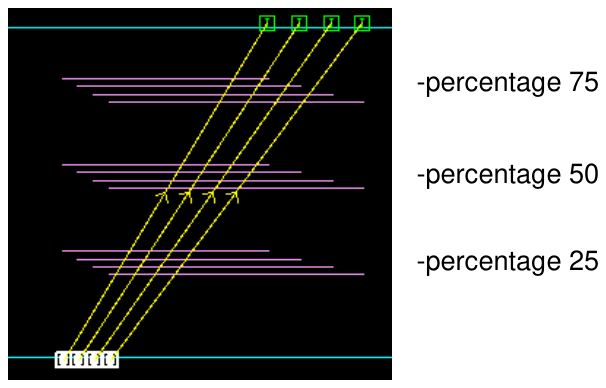
\includegraphics[width=0.92\textwidth]{gui-fig-166.png}
\caption{创建主干}
\label{fig:gui-166}
\end{figure}

为 \cmd{create\_trunk} 命令指定下列选项，以控制布线的创建方式。
\begin{itemize}
  \item 用 \opt{-direction horizontal | vertical} 指定该层的布线方向。默认情况下，命令沿首选方向（preferred direction）创建布线。
  \item 指定 \opt{-gravity driver}，使布线与线网的驱动端对齐。指定 \opt{-gravity load}，使布线与线网的负载端对齐。
  \item 用 \opt{-track\_numbers}、\opt{-track\_coords}、\opt{-track\_step} 与 \opt{-track\_ref\_bbox} 在线网包围盒内的指定轨道上创建布线。例如，要在从 (50,50) 到 (100,100) 的包围盒内创建布线，并从盒内第二条轨道开始，指定下列命令：
\begin{lstlisting}
icc2_shell> create_trunk -nets $nets -layer M3 \
   -track_ref_bbox {{50 50} {100 100}} -track_numbers 2
\end{lstlisting}
  \item 用 \opt{-avoid\_obstructions} 把布线放到下一条没有障碍（obstruction）的可用轨道上。默认情况下，若发现障碍，命令发出警告并跳过该线网。
  \item 用 \opt{-do\_not\_check\_shorts} 关闭对短路（short）与障碍的检查，并预览布线。
\end{itemize}

使用 \opt{-do\_not\_check\_shorts} 与 \opt{-avoid\_obstructions} 得到的版图结果如图~\ref{fig:gui-167} 所示。

\begin{figure}[htbp]
\centering
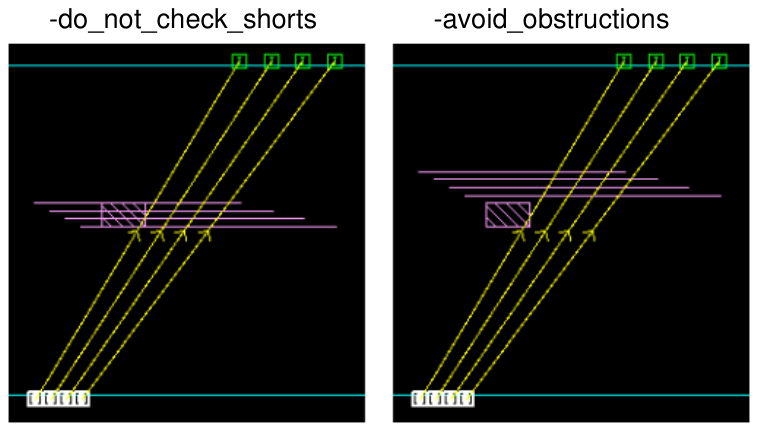
\includegraphics[width=0.92\textwidth]{gui-fig-167.png}
\caption{忽略障碍与短路，以及避开障碍}
\label{fig:gui-167}
\end{figure}

\begin{itemize}
  \item 用 \opt{-do\_not\_snap\_to\_track} 避免把布线吸附到轨道。
  \item 用 \opt{-num\_wires} 为每根线网创建不止一条布线。
  \item 用 \opt{-width} 把布线限制在特定轨道宽度上。默认情况下，布线创建在默认宽度的轨道上。
\end{itemize}

要在 GUI 中于单一金属层上沿一个方向创建布线主干：
\begin{enumerate}
  \item 选择 \textbf{Task > Trunk Routing}。
  \item 在 Trunk Routing 面板中单击 Setup。
  \item 在 Trunk Routing Setup 窗口中单击 \cmd{create\_trunk} 链接。
  \item 指定要为其创建布线主干的线网或线束。
  \item 指定创建布线主干所用的层。
  \item （可选）按需要填写其余字段。
  \item 单击 OK。
\end{enumerate}

\begin{figure}[htbp]
\centering
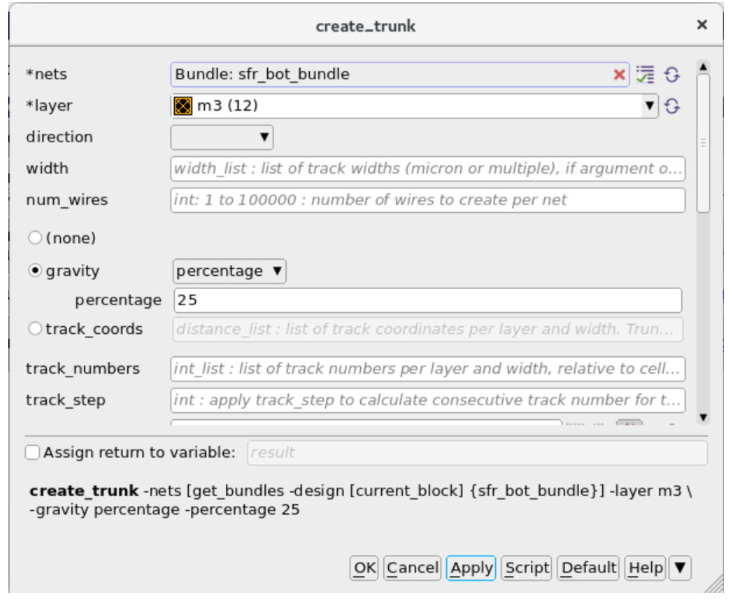
\includegraphics[width=0.92\textwidth]{gui-fig-168.png}
\caption{create\_trunk 命令的 GUI}
\label{fig:gui-168}
\end{figure}

\begin{figure}[htbp]
\centering
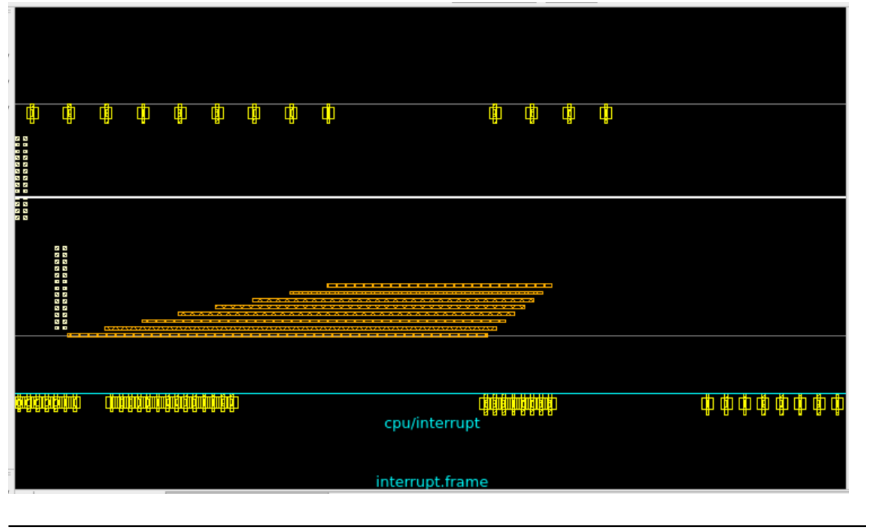
\includegraphics[width=0.92\textwidth]{gui-fig-169.png}
\caption{create\_trunk 命令的结果}
\label{fig:gui-169}
\end{figure}

\subsection{在同一轨道上沿一个方向创建布线段}
\subsubsection*{Creating Route Segments on the Same Track in One Direction}

要在同一条轨道上沿一个方向创建布线主干，按如下方式使用 \cmd{create\_trunk\_shared\_track} 命令：
\begin{lstlisting}
icc2_shell> create_trunk_shared_track -nets {sfr_small_bundle} -layer m3 \
   -track_coord 175 -width {0.4 0.6}
\end{lstlisting}

该命令为 \opt{-nets} 选项指定的每根线网创建一条布线段。本例中，\opt{-track\_coord} 指定决定布线起点的 x 或 y 坐标，并吸附到最近的轨道。\opt{-width} 指定放置这些布线的轨道宽度列表。

\begin{figure}[htbp]
\centering
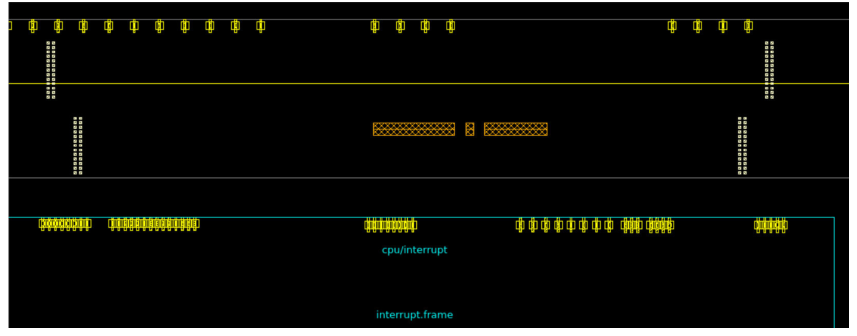
\includegraphics[width=0.92\textwidth]{gui-fig-170.png}
\caption{在同一轨道上沿一个方向创建布线段}
\label{fig:gui-170}
\end{figure}

为 \cmd{create\_trunk\_shared\_track} 命令指定下列选项，以控制布线的创建方式。
\begin{itemize}
  \item 用 \opt{-layer} 指定把管脚连接到布线所用的层。命令沿指定层的首选方向创建布线，并跳过非首选方向上的连接。
  \item 用 \opt{-direction horizontal | vertical} 指定该层的布线方向。默认情况下，命令沿首选方向创建布线。
  \item 用 \opt{-track\_numbers}、\opt{-track\_coords} 与 \opt{-track\_ref\_bbox} 在线网包围盒内的指定轨道上创建布线。
  \item 用 \opt{-avoid\_obstructions} 把布线放到下一条没有障碍的可用轨道上。默认情况下，若发现障碍，命令发出警告并跳过该线网。
  \item 用 \opt{-do\_not\_check\_shorts} 关闭对短路与障碍的检查，并预览布线。
  \item 用 \opt{-do\_not\_snap\_to\_track} 避免把布线吸附到轨道。
  \item 用 \opt{-track\_freedom} 允许在 \opt{-track\_ref\_bbox} 指定的边界之外，或在由指定线网的管脚连接所定义的包围盒之外创建布线。本选项与 \opt{-avoid\_obstructions} 一起使用。
  \item 用 \opt{-start\_pullback} 从起始管脚一侧缩短布线段，或用 \opt{-stop\_pullback} 在结束管脚一侧缩短布线段。若要把布线段延长而不是缩短，为该距离指定负值。
\end{itemize}

\opt{-start\_pullback} 与 \opt{-stop\_pullback} 既作用于信号，也作用于屏蔽（shielding）。只用 \opt{-shield\_pullback} 为屏蔽指定额外的回拉（pullback）。
\begin{itemize}
  \item 用 \opt{-gap} 在同一条轨道上的主干之间加入间隙。
  \item 用 \opt{-net\_bbox\_override} 指定创建布线段所用的包围盒。指定线网的实际包围盒被忽略，命令也不会尝试连接管脚。
  \item 用 \opt{-of\_cells} 或 \opt{-exclude\_cells} 在计算线网包围盒时包含或排除单元。在多扇出情形下使用这些选项，可以避免不必要的分支。
  \item 用 \opt{-create\_obstruction} 创建布线阻挡，而不创建布线形状。
  \item 用 \opt{-skip\_lib\_cells} 避免在库单元中搜索障碍。本选项与 \opt{-avoid\_obstructions} 一起使用。
  \item 用 \opt{-depth} 指定搜索障碍的层次（hierarchy）深度。默认搜索全部层次。本选项与 \opt{-avoid\_obstructions} 一起使用。
\end{itemize}

要在 GUI 中于同一条轨道上沿一个方向创建布线主干：
\begin{enumerate}
  \item 选择 \textbf{Task > Trunk Routing}。
  \item 在 Trunk Routing 面板中单击 Setup。
  \item 在 Trunk Routing Setup 窗口中单击 \cmd{create\_trunk\_shared\_track} 链接。
  \item 指定要为其创建布线主干的线网或线束。
  \item 指定创建布线主干所用的层。
  \item （可选）按需要填写其余字段。
  \item 单击 OK。
\end{enumerate}

\begin{figure}[htbp]
\centering
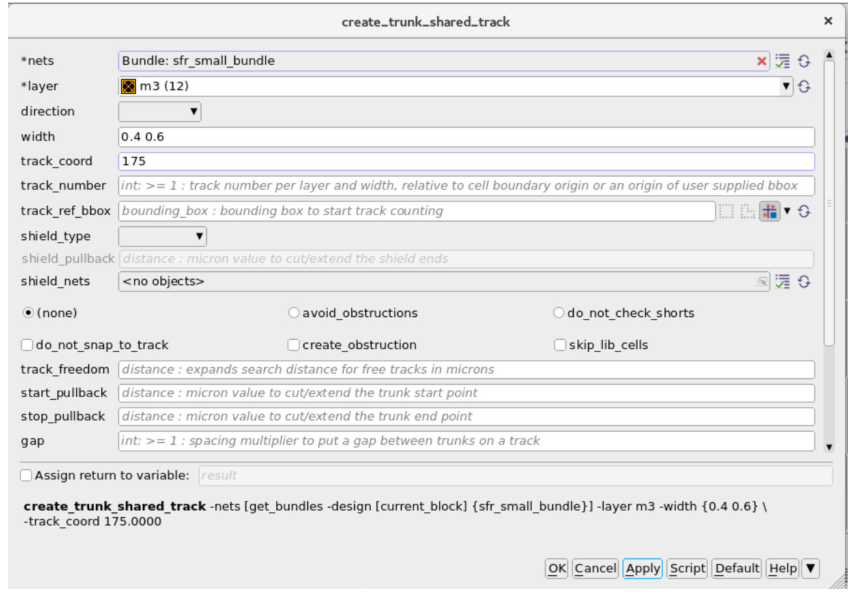
\includegraphics[width=0.92\textwidth]{gui-fig-171.png}
\caption{create\_trunk\_shared\_track 命令的 GUI}
\label{fig:gui-171}
\end{figure}

\begin{figure}[htbp]
\centering
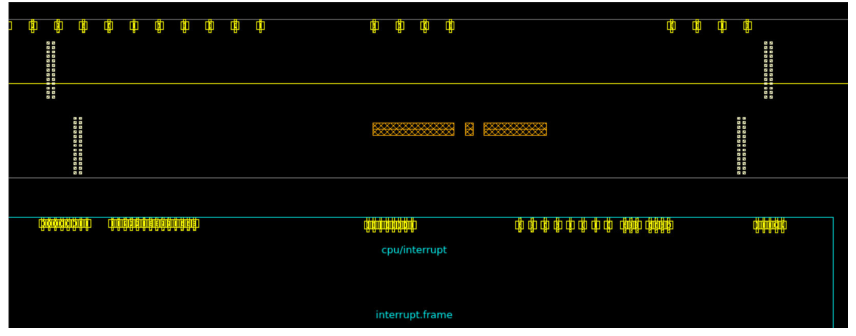
\includegraphics[width=0.92\textwidth]{gui-fig-172.png}
\caption{create\_trunk\_shared\_track 命令的结果}
\label{fig:gui-172}
\end{figure}

\subsection{从管脚连接到已有布线段}
\subsubsection*{Creating Routes From Pins to Existing Route Segments}

要在管脚与已有布线段之间创建布线，按如下方式使用 \cmd{create\_trunk\_pin\_to\_trunk} 命令：
\begin{lstlisting}
icc2_shell> create_bundle b1 [get_nets {net1 net2 net3 net4}]
icc2_shell> create_trunk_pin_to_trunk -nets b1
\end{lstlisting}

该命令在已有布线主干与该主干上线网所关联的最近管脚之间创建一条布线段，如图~\ref{fig:gui-173} 所示。本例中，布线创建在与管脚相同的层上。

\begin{figure}[htbp]
\centering
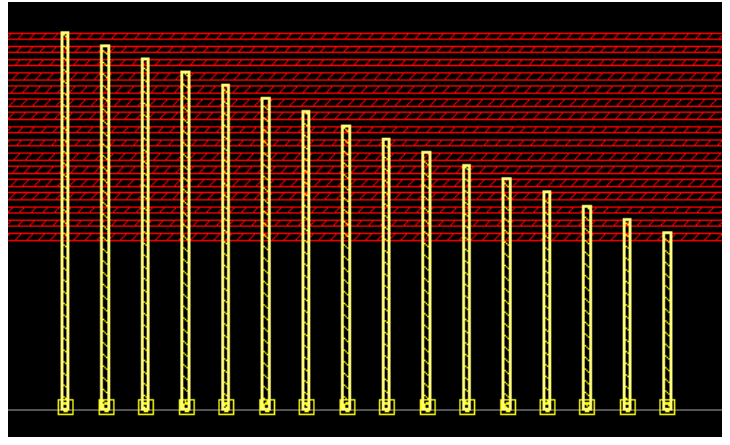
\includegraphics[width=0.92\textwidth]{gui-fig-173.png}
\caption{把管脚连接到已有布线}
\label{fig:gui-173}
\end{figure}

为 \cmd{create\_trunk\_pin\_to\_trunk} 命令指定下列选项，以控制布线的创建方式。
\begin{itemize}
  \item 用 \opt{-layer} 指定把管脚连接到布线所用的层。命令沿指定层的首选方向创建布线，并跳过非首选方向上的连接。
  \item 用 \opt{-direction horizontal | vertical} 沿指定方向创建布线段。另一方向上的连接被跳过。
  \item 用 \opt{-do\_not\_snap\_to\_track} 避免把布线吸附到轨道。
  \item 用 \opt{-avoid\_obstructions} 把布线放到下一条没有障碍的可用轨道上。默认情况下，若发现障碍，命令发出警告并跳过该线网。
  \item 用 \opt{-do\_not\_check\_shorts} 关闭对短路与障碍的检查，并预览布线。
  \item 用 \opt{-cluster\_proximity} 减少从主干创建的布线形状数量。用本选项指定一个以微米为单位的范围，把该范围内单独的管脚到主干形状合并为单一形状。命令会从主干创建布线段，但可能不完成到管脚的连接。
\end{itemize}

为聚类邻近距离指定三个不同值之后的版图结果如图~\ref{fig:gui-174} 所示。

\begin{figure}[htbp]
\centering
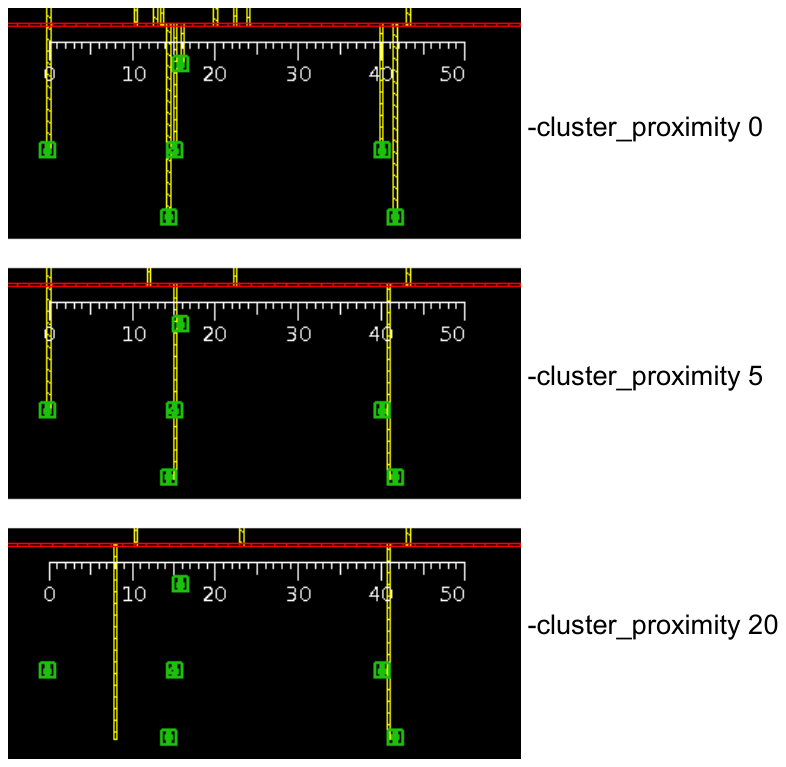
\includegraphics[width=0.92\textwidth]{gui-fig-174.png}
\caption{聚类邻近距离}
\label{fig:gui-174}
\end{figure}

要补上缺少的连接，再次运行 \cmd{create\_trunk\_pin\_to\_trunk}，并指定正交方向上的层。下面的示例先创建垂直布线，然后再次调用 \cmd{create\_trunk\_pin\_to\_trunk}，以完成到管脚的连接。
\begin{lstlisting}
icc2_shell> create_trunk_pin_to_trunk -nets $nets -layer METAL2 \
   -cluster_proximity 40
icc2_shell> create_trunk_pin_to_trunk -nets $nets -layer METAL3
\end{lstlisting}

要在 GUI 中于管脚与已有布线段之间创建布线：
\begin{enumerate}
  \item 选择 \textbf{Task > Trunk Routing}。
  \item 在 Trunk Routing 面板中单击 Setup。
  \item 在 Trunk Routing Setup 窗口中单击 \cmd{create\_trunk\_pin\_to\_trunk} 链接。
  \item 指定要为其创建布线主干的线网。
  \item （可选）按需要填写其余字段。
  \item 单击 OK。
\end{enumerate}

\begin{figure}[htbp]
\centering
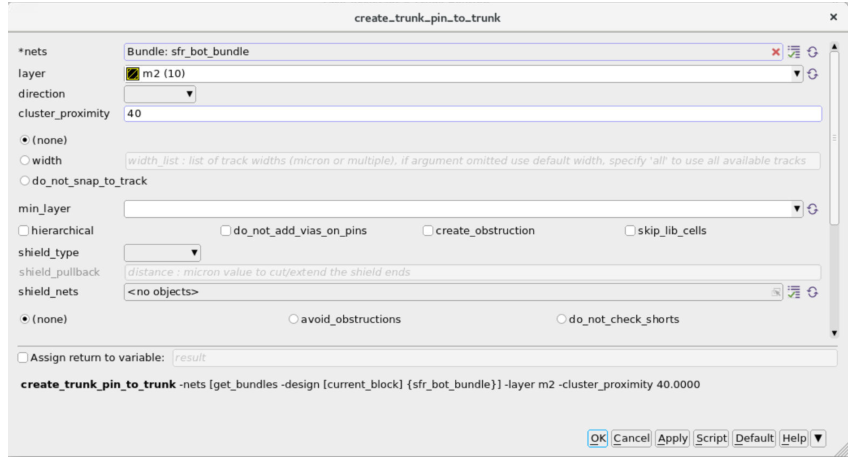
\includegraphics[width=0.92\textwidth]{gui-fig-175.png}
\caption{create\_trunk\_pin\_to\_trunk 命令的 GUI}
\label{fig:gui-175}
\end{figure}

\begin{figure}[htbp]
\centering
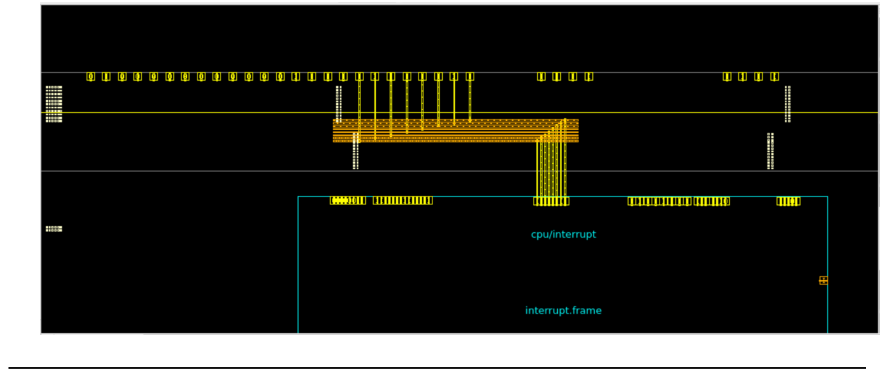
\includegraphics[width=0.92\textwidth]{gui-fig-176.png}
\caption{create\_trunk\_pin\_to\_trunk 命令的结果}
\label{fig:gui-176}
\end{figure}

\subsection{从管脚到管脚创建布线}
\subsubsection*{Creating Routes From Pin to Pin}

要在管脚之间创建布线段，按如下方式使用 \cmd{create\_trunk\_pin\_to\_pin} 命令：
\begin{lstlisting}
icc2_shell> create_bundle b1 [get_nets {net1 net2 net3 net4}]
icc2_shell> create_trunk_pin_to_pin -nets b1 \
   -extensions {0.67 1.0 0.33} -layer_legs {M4 M3 M4}
\end{lstlisting}

该命令产生的版图结果如图~\ref{fig:gui-177} 所示。

\begin{figure}[htbp]
\centering
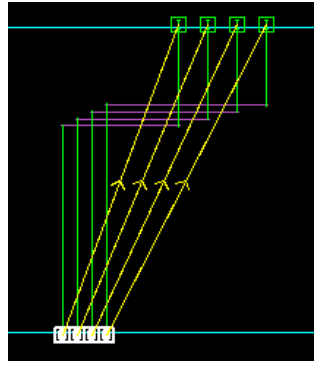
\includegraphics[width=0.92\textwidth]{gui-fig-177.png}
\caption{管脚到管脚的布线主干}
\label{fig:gui-177}
\end{figure}

本例中，\opt{-extensions} 指定各布线段的相对长度，从驱动管脚开始，到负载管脚结束。要反转某一段的方向，为延伸值指定负数。要从目标管脚开始布线，见下面列表中对 \opt{-start\_from} 的说明。各段对应的层用 \opt{-layer\_legs} 指定。

为 \cmd{create\_trunk\_pin\_to\_pin} 命令指定下列选项，以控制布线的创建方式。
\begin{itemize}
  \item 用 \opt{-layer\_legs} 指定给定层所用的具体轨道宽度。例如，下列命令只把布线放在 M2 与 M3 上宽度为 0.4 或 0.8 的轨道上。要使用任意可用轨道宽度，把 \cmd{\{0.4 0.8\}} 换成 \cmd{all} 参数。默认情况下，命令只把布线放在默认宽度的轨道上。
\begin{lstlisting}
icc2_shell> create_trunk_pin_to_pin -nets $nets \
   -layer_legs {{METAL2 {0.4 0.8}} {METAL3 {0.4 0.8}}} \
   -extensions {1 1}
\end{lstlisting}
  \item 用 \opt{-extensions} 指定每一段的长度。该选项接受一个延伸值列表，列表中的每个元素指定布线中一段的长度。延伸值可以指定为线网包围盒的分数、线网包围盒的百分比、以微米为单位的距离，或用户定义的单位。
  \item 用 \opt{-layer\_legs} 与一个层列表一起指定每一段所用的层。每一层对应 \opt{-extensions} 所指定的一段。
  \item 用 \opt{-net\_bbox\_override} 指定创建布线段所用的包围盒。指定线网的实际包围盒被忽略，命令也不会尝试连接管脚。
  \item 用 \opt{-start\_from} 指定开始布线的管脚的相对位置。
\end{itemize}

在下面的示例中，第一条命令从位于图下方的源管脚开始布线，得到左侧的版图结果；第二条命令从位于图上方的目标管脚开始布线，得到右侧的版图结果。
\begin{lstlisting}
icc2_shell> create_trunk_pin_to_pin -nets b4 \
   -extensions {0.25 1.0 0.75} -layer_legs {M4 M3 M4}
icc2_shell> create_trunk_pin_to_pin -nets b4 \
   -extensions {0.25 1.0 0.75} -layer_legs {M4 M3 M4} \
   -start_from high_y
\end{lstlisting}

\begin{figure}[htbp]
\centering
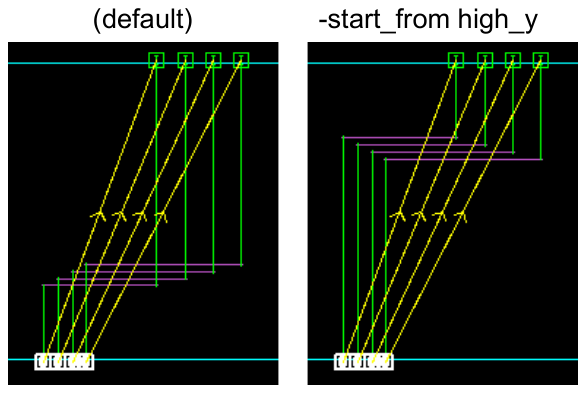
\includegraphics[width=0.92\textwidth]{gui-fig-178.png}
\caption{起始位置}
\label{fig:gui-178}
\end{figure}

\begin{itemize}
  \item 用 \opt{-do\_not\_snap\_to\_track} 避免把布线吸附到轨道。
  \item 用 \opt{-do\_not\_check\_shorts} 关闭对短路与障碍的检查，并预览布线。
  \item 用 \opt{-start\_pullback} 从起始管脚一侧缩短布线段，或用 \opt{-stop\_pullback} 在结束管脚一侧缩短布线段。若要把布线段延长而不是缩短，为该距离指定负值。
\end{itemize}

\opt{-start\_pullback} 与 \opt{-stop\_pullback} 既作用于信号，也作用于屏蔽。只用 \opt{-shield\_pullback} 为屏蔽指定额外的回拉。

要在 GUI 中于管脚之间创建布线段：
\begin{enumerate}
  \item 选择 \textbf{Task > Trunk Routing}。
  \item 在 Trunk Routing 面板中单击 Setup。
  \item 在 Trunk Routing Setup 窗口中单击 \cmd{create\_trunk\_pin\_to\_pin} 链接。
  \item 指定要为其创建布线主干的线网或线束。
  \item 指定创建布线主干所用的层。
  \item 在 extensions 文本框中指定布线的相对长度。
  \item （可选）按需要填写其余字段。
  \item 单击 OK。
\end{enumerate}

\begin{figure}[htbp]
\centering
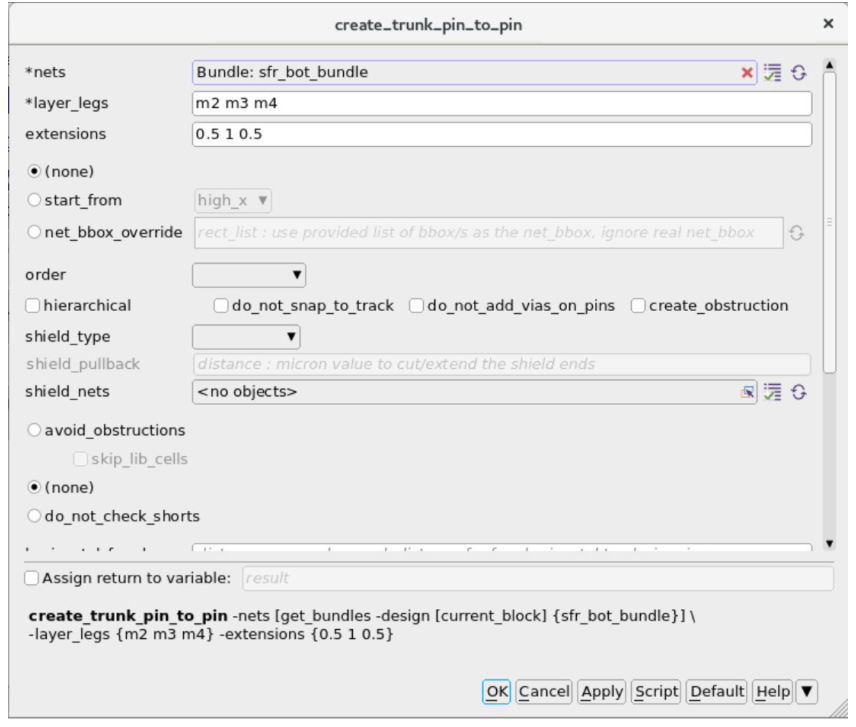
\includegraphics[width=0.92\textwidth]{gui-fig-179.png}
\caption{create\_trunk\_pin\_to\_pin 命令的 GUI}
\label{fig:gui-179}
\end{figure}

\begin{figure}[htbp]
\centering
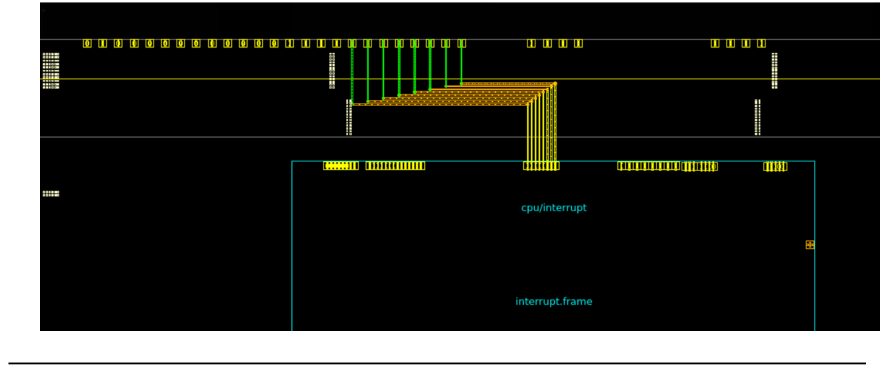
\includegraphics[width=0.92\textwidth]{gui-fig-180.png}
\caption{create\_trunk\_pin\_to\_pin 命令的结果}
\label{fig:gui-180}
\end{figure}

\subsection{从拓扑边创建布线}
\subsubsection*{Creating Routes From Topology Edges}

要从拓扑边（topology edge）创建布线，按如下方式使用 \cmd{create\_trunk\_topology} 命令：
\begin{lstlisting}
icc2_shell> set shape_layers {{m2 50% 0} {m3 100% 0} {m4 50% 0}}
icc2_shell> create_topology_plan -name TP1 -objects \
   [get_bundles sfr_bot_bundle]
icc2_shell> create_topology_node -plan TP1 -name N1 -constraint_type bbox \
   -objects [get_ports sfr_data_out* ]
icc2_shell> create_topology_node -plan TP1 -name N2 \
   -constraint_type bbox -objects [get_pins cpu/interrupt/sfr_data_out* ]
icc2_shell> create_topology_edge -name E12 -plan TP1 \
   -nodes {TP1/N1 TP1/N2} -shape_layers $shape_layers \
   -objects [get_nets sfr_data_out*]
icc2_shell> create_trunk_topology -edge TP1/E12
\end{lstlisting}

上面这一组命令创建的版图结果如图~\ref{fig:gui-181} 所示。

\begin{figure}[htbp]
\centering
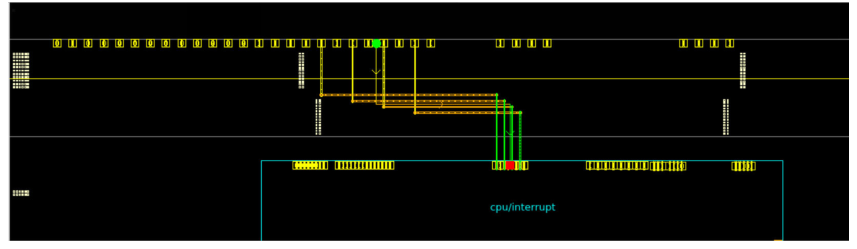
\includegraphics[width=0.92\textwidth]{gui-fig-181.png}
\caption{从拓扑边布线}
\label{fig:gui-181}
\end{figure}

本例中，\opt{-edge} 指定要为其创建布线的拓扑边名称。

为 \cmd{create\_trunk\_topology} 命令指定下列选项，以控制布线的创建方式。
\begin{itemize}
  \item 用 \opt{-plan} 指定要为其创建布线的拓扑规划（topology plan）名称或集合。
  \item 用 \opt{-avoid\_obstructions} 把布线放到下一条没有障碍的可用轨道上。默认情况下，若发现障碍，命令发出警告并跳过该线网。
  \item 用 \opt{-do\_not\_check\_shorts} 关闭对短路与障碍的检查，并预览布线。
  \item 用 \opt{-do\_not\_snap\_to\_track} 避免把布线吸附到轨道。
  \item 用 \opt{-do\_not\_add\_vias\_on\_pins} 避免在管脚上添加通孔。
  \item 用 \opt{-horizontal\_freedom} 或 \opt{-vertical\_freedom} 在水平或垂直方向上扩大布线可以挪动的区域。
  \item 用 \opt{-start\_pullback} 从起始管脚一侧缩短布线段，或用 \opt{-stop\_pullback} 在结束管脚一侧缩短布线段。若要把布线段延长而不是缩短，为该距离指定负值。
\end{itemize}

\opt{-start\_pullback} 与 \opt{-stop\_pullback} 既作用于信号，也作用于屏蔽。只用 \opt{-shield\_pullback} 为屏蔽指定额外的回拉。
\begin{itemize}
  \item 用 \opt{-skip\_lib\_cells} 避免在库单元中搜索障碍。本选项与 \opt{-avoid\_obstructions} 一起使用。
\end{itemize}

要在 GUI 中从拓扑边创建布线段：
\begin{enumerate}
  \item 选择 \textbf{Task > Trunk Routing}。
  \item 在 Trunk Routing 面板中单击 Setup。
  \item 在 Trunk Routing Setup 窗口中单击 \cmd{create\_trunk\_topology} 链接。
  \item 指定要为其创建布线的拓扑规划名称或边。
  \item （可选）按需要填写其余字段。
  \item 单击 OK。
\end{enumerate}

\begin{figure}[htbp]
\centering
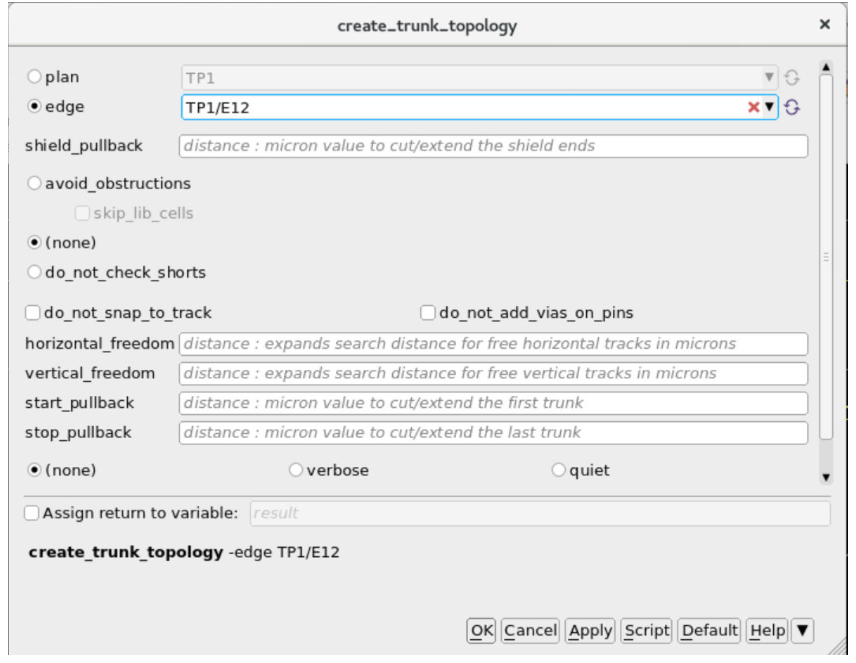
\includegraphics[width=0.92\textwidth]{gui-fig-182.png}
\caption{create\_trunk\_topology 命令的 GUI}
\label{fig:gui-182}
\end{figure}

\begin{figure}[htbp]
\centering
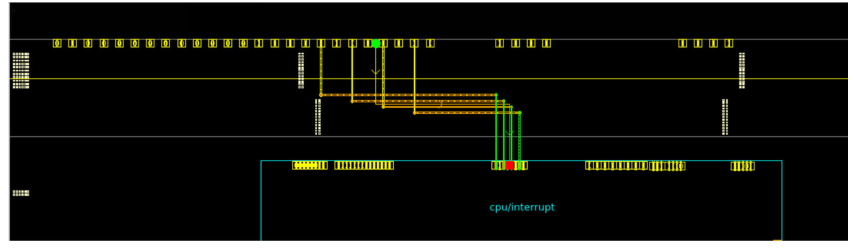
\includegraphics[width=0.92\textwidth]{gui-fig-183.png}
\caption{create\_trunk\_topology 命令的结果}
\label{fig:gui-183}
\end{figure}

\subsection{布线区域包围盒}
\subsubsection*{Routing Area Bounding Box}

默认情况下，\cmd{create\_trunk} 与 \cmd{create\_trunk\_pin\_to\_pin} 在由源管脚与目标管脚形成的包围盒内创建布线，如图~\ref{fig:gui-184} 所示。

\begin{figure}[htbp]
\centering
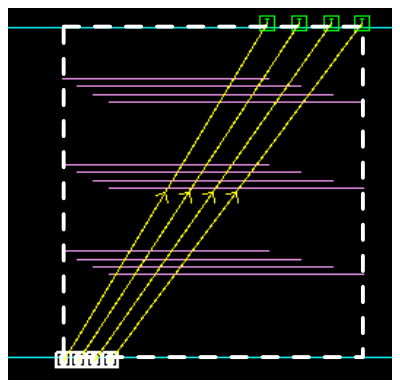
\includegraphics[width=0.92\textwidth]{gui-fig-184.png}
\caption{布线主干的默认包围盒}
\label{fig:gui-184}
\end{figure}

要在指定包围盒内创建布线主干，为 \cmd{create\_trunk} 与 \cmd{create\_trunk\_pin\_to\_pin} 指定 \opt{-net\_bbox\_override}。下面的示例在由 (100,100) 与 (200,200) 围成的盒子内，为 \cmd{net1} 与 \cmd{net2} 创建布线主干。
\begin{lstlisting}
icc2_shell> create_trunk -nets {net1 net2} -layer METAL3 \
   -net_bbox_override {{100 100} {200 200}}
\end{lstlisting}

\subsection{屏蔽线网}
\subsubsection*{Shielding Nets}

可以用 \opt{-shield\_nets} 与 \opt{-shield\_type} 选项，配合 \cmd{create\_trunk}、\cmd{create\_trunk\_pin\_to\_trunk} 或 \cmd{create\_trunk\_pin\_to\_pin} 创建屏蔽线网。\opt{-shield\_type} 支持布线上的全屏蔽（full）、部分屏蔽（partial）或端帽屏蔽（cap）。屏蔽线网在各线网之间共享。屏蔽线网的顺序与位置相对 x 轴和 y 轴。因此，低端屏蔽线网总是从较低的 x 或 y 位置开始，高端屏蔽线网从较高的 x 或 y 位置开始。工具支持全交错屏蔽（full interleaved shielding）与半交错屏蔽（half interleaved shielding）。

\opt{-start\_pullback} 与 \opt{-stop\_pullback} 既作用于信号，也作用于屏蔽。只用 \opt{-shield\_pullback} 为屏蔽指定额外的回拉。

图~\ref{fig:gui-185} 给出没有屏蔽线网时的默认版图结果，以及运行下列命令创建屏蔽线网之后的版图结果。由 \cmd{\$nets} 指定的非屏蔽线网被高亮，供对照。
\begin{lstlisting}
icc2_shell> create_trunk -nets $nets -layer M3 \
   -shield_nets VDD -shield_type full
\end{lstlisting}

\begin{figure}[htbp]
\centering
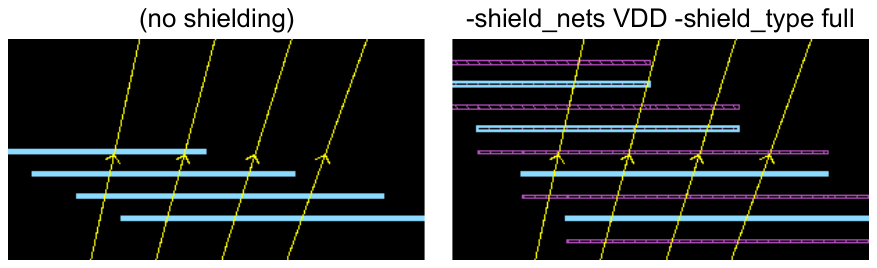
\includegraphics[width=0.92\textwidth]{gui-fig-185.png}
\caption{屏蔽线网}
\label{fig:gui-185}
\end{figure}

图~\ref{fig:gui-186} 与图~\ref{fig:gui-187} 给出全屏蔽 \cmd{\{VCC VSS\}} 的共享线网示例，分别采用河流式拐角（river corner）与交叉式拐角（cross corner）。这两幅图是运行下列命令创建屏蔽线网之后的结果。
\begin{lstlisting}
icc2_shell> create_trunk_pin_to_pin -nets $nets \
   -extensions {0.5 1.0 0.5} -layer_legs {M3 M2 M3} \
   -shield_type full -shield_nets VCC VSS
\end{lstlisting}

\begin{figure}[htbp]
\centering
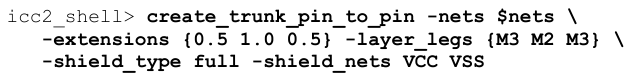
\includegraphics[width=0.92\textwidth]{gui-fig-186.png}
\caption{河流式拐角的全交错屏蔽（VCC 为绿色，VSS 为蓝色）}
\label{fig:gui-186}
\end{figure}

\begin{figure}[htbp]
\centering
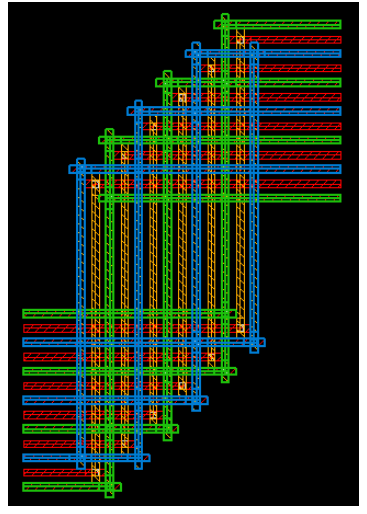
\includegraphics[width=0.92\textwidth]{gui-fig-187.png}
\caption{交叉式拐角的全交错屏蔽（VCC 为绿色，VSS 为蓝色）}
\label{fig:gui-187}
\end{figure}

图~\ref{fig:gui-188} 与图~\ref{fig:gui-189} 给出半屏蔽 \cmd{\{VCC VSS\}} 的共享线网示例，分别采用河流式拐角与交叉式拐角。这两幅图是运行下列命令创建屏蔽线网之后的结果。
\begin{lstlisting}
icc2_shell> create_trunk_pin_to_pin -nets $nets \
   -extensions {0.5 1.0 0.5} -layer_legs {M3 M2 M3} \
   -shield_type half -shield_nets VCC VSS
\end{lstlisting}

\begin{figure}[htbp]
\centering
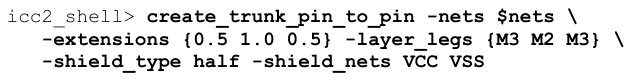
\includegraphics[width=0.92\textwidth]{gui-fig-188.png}
\caption{河流式拐角的半交错屏蔽（VCC 为绿色，VSS 为蓝色）}
\label{fig:gui-188}
\end{figure}

\begin{figure}[htbp]
\centering
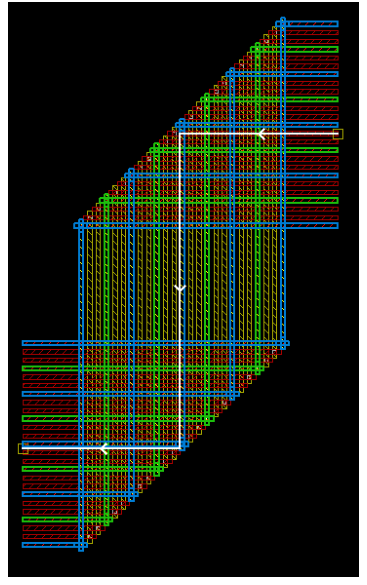
\includegraphics[width=0.92\textwidth]{gui-fig-189.png}
\caption{交叉式拐角的半交错屏蔽（VCC 为绿色，VSS 为蓝色）}
\label{fig:gui-189}
\end{figure}

要使 \cmd{create\_trunk\_pin\_to\_pin} 使用已有的 PG 网格（PG mesh）做屏蔽，需保证 PG 网格线宽与其下方轨道的宽度一致，见图~\ref{fig:gui-190}。

\begin{figure}[htbp]
\centering
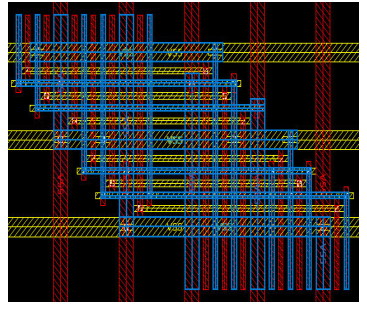
\includegraphics[width=0.92\textwidth]{gui-fig-190.png}
\caption{与地网格共享的全屏蔽 \{VSS\}}
\label{fig:gui-190}
\end{figure}

% 第 14 章 Creating Routes（续）

\section{在布线上添加缓冲器}
\subsection*{Adding Buffers on Routes}

Add Buffer on Route 工具可以沿指定线网的布线添加缓冲器（buffer）。

要启动 Add Buffer on Route 工具，单击 Command search 按钮，并在搜索框中输入 \cmd{add\_buffer\_on\_route}。

下图中，1 是命令搜索图标，2 是输入命令的文本框，3 显示与搜索文本匹配的命令。

Add Buffer on Route 对话框随即打开，分为以下部分：
\begin{itemize}
  \item 顶部区域（Top region）
  \item Basic 选项卡
  \item Advanced 选项卡
\end{itemize}

对话框中以红色显示、或前面带星号的字段为必填。尚未提供的必填信息会显示在该对话框底部。

表~\ref{tab:gui-buf-route} 列出 Add Buffer on Route 对话框的选项。

\begin{longtable}{@{}p{0.32\textwidth}p{0.62\textwidth}@{}}
\caption{Add Buffer on Route 对话框选项}
\label{tab:gui-buf-route}\\
\toprule
字段 & 说明 \\
\midrule
\endfirsthead
\caption{Add Buffer on Route 对话框选项（续）}\\
\toprule
字段 & 说明 \\
\midrule
\endhead
\midrule
\multicolumn{2}{r}{\small 下页继续} \\
\endfoot
\bottomrule
\endlastfoot
Nets & 指定要插入缓冲器的线网。 \\
Location & 指定缓冲器或反相器对（inverter pair）单元所在位置的中心点坐标。 \\
Specified buffers & 指定缓冲器或反相器对单元的中心点坐标，以及它们的名称和库单元。 \\
Specified bus buffers &
指定总线缓冲器（bus buffer）或反相器对单元的中心点坐标，以及它们的名称和库单元。格式为 \cmd{\{bus\_buffer\_pattern1 lib\_cell1 x1 y1 bus\_buffer\_pattern2 lib\_cell2 x2 y2 ...\}}。 \\
Repeater distance & 指定沿布线插入的各个缓冲器之间的距离，单位为用户单位（user unit）。 \\
\multicolumn{2}{@{}l}{\textbf{Mode}} \\
\addlinespace
Repeater distance length ratio &
以总布线长度的比例，指定沿布线插入的各个缓冲器之间的距离。 \\
Point & 指定版图视图上的点坐标。 \\
Layer & 从下拉列表中选择一层。 \\
Detect layer & 指定工具自动检测位置坐标所在的层。 \\
Name & 指定所添加缓冲器的名称。 \\
Lib Cell & 指定用作中继器（repeater）的库单元对象。 \\
Distance & 指定中继器距离，即各个缓冲器之间的距离。 \\
Scale & 按该层指定的缩放因子，缩放缓冲器之间的距离。 \\
Ratio & 各个缓冲器之间的距离与总布线长度之比。 \\
Scaled by width &
按该层默认宽度与实际布线宽度之比，缩放缓冲器之间的距离。 \\
\multicolumn{2}{@{}l}{\textbf{Basic 选项卡}} \\
\addlinespace
Only global routed nets & 允许在全局布线的线网（global routed net）上插入缓冲器。 \\
Punch port &
即使拓扑（topology）与逻辑层次中的网表连接不同，也允许在布线段上插入缓冲器。 \\
Respect voltage area &
在电压区域（voltage area）的层次内插入缓冲器，使缓冲器在版图上物理地位于该层次内部。 \\
Reference Cells > Voltage Area, Lib Cell &
指定在给定电压区域中使用的库单元对象。 \\
Respect gas station &
仅在指定供电线网的加油站（gas station）内、并沿布线添加缓冲器。这些加油站的 \cmd{is\_primary} 属性为 false。 \\
Physical feedthrough &
指定可以添加缓冲器的电压区域，即使它们只是物理贯通（physical-only feedthrough）。 \\
Select MV buffers > Voltage Area, Single Rail, Dual Rail &
指定在给定电压区域中使用的单电源轨（single-rail）与双电源轨（dual-rail）库单元对象。这些是多电压缓冲器（multi-voltage buffer，MV buffer）。 \\
Prefix > Bus cell &
指定由 \opt{-user\_specified\_bus\_buffers} 选项添加的新缓冲器所用的前缀。 \\
Prefix > Cell &
指定插入网表的新缓冲器所用的前缀。默认情况下，命令使用 \cmd{eco\_cell} 作为前缀。 \\
Prefix > Net &
指定向网表插入缓冲器时新建线网所用的前缀。默认情况下，命令使用 \cmd{eco\_net} 作为前缀。 \\
\multicolumn{2}{@{}l}{\textbf{Advanced 选项卡}} \\
\addlinespace
Snap to sites & 把新添加的缓冲器吸附到最近的位点（site）。 \\
On top hierarchy &
把缓冲器加到层次最高层的线网上。默认情况下，缓冲器加在其所驱动管脚的最低公共祖先层次中。 \\
Verbose & 显示详细消息。 \\
Respect blockages &
指定不在布局阻挡（placement blockage）、软宏或硬宏内添加缓冲器。 \\
Spare cell aware &
在冻结硅（freeze-silicon）模式下启用感知备用单元（spare cell）的功能。 \\
Insertion over cell > Allowed &
指定可以在其中添加中继器的软宏或硬宏实例。本选项与 Respect blockages 选项一起使用。 \\
Insertion over cell > Not allowed &
指定不允许添加中继器的软宏或硬宏实例。 \\
Max distance > Location to route &
指定给定位置与布线之间的最大水平或垂直距离，单位为用户单位。本选项与 Respect gas station 选项一起使用。启用 Respect gas station 时，缓冲器必须加在加油站内部。 \\
Max distance > Incomplete route & 定义不完整布线的最大搜索距离。 \\
Max distance > Route to gas station &
指定添加缓冲器的加油站到布线的距离。若未指定本选项，加油站必须位于布线上。 \\
Max distance > Spare cell &
在冻结硅模式下，指定新添加的缓冲器与备用单元之间的最大距离。 \\
First distance -- Length &
指定驱动管脚与沿布线引入的第一个缓冲器之间的距离，单位为用户单位。本选项与 Repeater distance 或 Repeater distance length ratio 选项一起使用。 \\
First distance -- Ratio &
以总布线长度的比例，指定驱动管脚与沿布线引入的第一个缓冲器之间的距离。本选项与 Repeater distance length ratio 选项一起使用。 \\
\end{longtable}

表~\ref{tab:gui-gas-station} 给出加油站示例。

\begin{table}[htbp]
\centering
\caption{加油站示例}
\label{tab:gui-gas-station}
\begin{tabularx}{\textwidth}{@{}l X@{}}
\toprule
情形 & 说明 \\
\midrule
启用 Respect gas station &
缓冲器必须加在加油站内部。 \\
Max distance > Route to gas station &
允许放大加油站，因此即使加油站不在布线上，仍可以添加缓冲器。 \\
示例流程 &
\begin{minipage}[t]{\linewidth}
\begin{enumerate}
  \item 选择线网 \cmd{p0}。
  \item 添加用户指定的缓冲器。
\end{enumerate}
\end{minipage} \\
\bottomrule
\end{tabularx}
\end{table}

下图给出结果。

% ============================================================
\section{估算点到点电阻}
\subsection*{Estimating Point-to-Point Resistance}

要计算当前设计中两点（管脚或端口）之间的电阻（resistance），使用 \cmd{estimate\_resistance} 命令。

在该命令中，可以用多种方式指定起点与终点：
\begin{itemize}
  \item 使用 \opt{-net}。本选项只适用于仅有两个管脚或端口、且每个管脚或端口只有一个端子的线网。
  \item 使用 \opt{-pins}。本选项适用于有两个以上管脚或端口的线网。必须在命令中指定确切的管脚和端口，命令才能测量这些指定点之间的电阻。
  \item 使用 \opt{-shapes}。本选项适用于测量复杂结构中任意线段的电阻，例如电源地管脚与网格（mesh）的连接。为兼顾性能，避免把整个网格作为一组形状传入。
\end{itemize}

使用 \opt{-shapes} 时，需指定起点及其所在层，以及终点及其所在层。

用 \opt{-quiet} 与 \opt{-verbose} 分别在控制台上抑制消息，或详细打印消息。

下面的命令估算指定单元上 VDD 管脚之间的电阻：
\begin{lstlisting}
icc2_shell> estimate_resistance -pins "INV_279/VDD U27/VDD"
\end{lstlisting}


% 第 15 章 Creating Anchors
\bichapter{创建 Anchor}{Creating Anchors}
\label{chap:gui-anchor}

Anchor 把一个设计对象固定到另一个对象上。被固定的对象是从属对象（dependent object），它所依附的对象是锚点对象（anchor object）。移动锚点对象时，固定在它上面的从属对象一起移动。移动从属对象时，它会弹回锚点位置。

在 IC Compiler II GUI 中选择 \textbf{Create > Anchor}，即可打开创建工具。该工具提供：
\begin{itemize}
  \item Anchor type：指定固定方式，可以只固定 X、只固定 Y，或同时固定 X 与 Y。
  \item Dependent：指定从属对象。
  \item Anchor：指定锚点对象。
  \item Position Reference：指定从属对象与锚点对象的位置参考。
  \item Offset：指定从属对象相对锚点对象的 X、Y 偏移，默认是 \cmd{\{0,0\}}。
\end{itemize}

也可以在层次内部创建 anchor。在 Layout settings 面板中启用 deep selection 并提高 view level，然后即可在层次内部点选从属对象和锚点对象。

\begin{noteBox}
从属对象的层次级别必须等于或低于锚点对象的层次级别。
\end{noteBox}

表~\ref{tab:gui-anchor} 是 CreateAnchor 工具中交互编辑的约定。

\begin{table}[htbp]
\centering
\caption{CreateAnchor 工具的交互约定}
\label{tab:gui-anchor}
\begin{tabularx}{\textwidth}{@{}l X@{}}
\toprule
事件 & 动作 \\
\midrule
单击或拖拽 & 设置矩形一角，或创建 Anchor \\
双击或按 Enter & 在当前位置创建 Anchor \\
中键单击 & 激活笔势菜单 \\
右键单击 & 显示上下文菜单 \\
F1 & 在重叠对象中向前循环 \\
Shift+F1 & 在重叠对象中向后循环 \\
Escape & 若有未完成的更改则取消；否则退出工具 \\
\bottomrule
\end{tabularx}
\end{table}

% 第 16 章 Creating Cell
\bichapter{创建单元}{Creating Cell}
\label{chap:gui-cell}

可以从 IC Compiler II GUI 创建单元（原型块或完整芯片）。也可以不使用 edit-in-place，直接创建层次块。

选择 \textbf{Create > Cell}，或使用创建单元的鼠标工具。Create Cell 工具随即出现。

\section{创建层次块}
\subsection*{Creating a Hierarchical Block}

创建层次实例或块：
\begin{enumerate}
  \item 在 Layout settings 面板中启用 deep selection，并提高 Level。
  \item 选择 \textbf{Create > Cell}，打开 Create Cell 工具。
  \item 单击 New Block Cell 图标以创建新块，或单击 Add Block Cell 图标以创建已有块的实例。
  \item 在 Library 栏指定库。
  \item 指定 Reference Block 与单元实例名。
  \item 在 Design type 栏指定设计类型，例如 die、diode、module。
  \item 指定 Z 偏移，也可以设为 Auto。
  \item 拖出一个矩形以创建新块。若要创建已有单元的实例，把形状拖到所需位置。
\end{enumerate}

% 第 17 章 Creating Persistent Annotations
\bichapter{创建持久标注}{Creating Persistent Annotations}
\label{chap:gui-anno}

要创建保存在数据库中的持久标注（persistent annotation，包括形状、文本和符号），使用 \cmd{create\_annotation\_shape}、\cmd{create\_annotation\_text} 和 \cmd{create\_annotation\_symbol} 命令。也可以用 Create Annotation 工具（\textbf{Create > Annotation}）来创建。

在 Create Annotation 工具中选中 Attach 复选框后，指针下方的对象会被预先选中。在这样的对象上单击时，标注会附着或锚定到该对象。移动该对象时，标注随之移动。

本章包括以下主题：
\begin{itemize}
  \item 创建标注形状
  \item 创建标注符号
  \item 创建标注文本
  \item 编辑持久标注
  \item 删除持久标注
\end{itemize}

\section{创建标注形状}
\subsection*{Creating Annotation Shapes}

使用 \cmd{create\_annotation\_shape} 命令创建标注形状，类型为圆形（circle）、直线（line）、矩形（rectangle）和多边形（polygon），并可带可选的文本标签。该命令的更多信息见 man 页。

也可以用 Create Annotation 工具创建标注形状。用该工具可以指定类型（circle、rectangle 等）、样式（style，包括填充图案 fill pattern、线宽 line width、颜色等）、标签，以及标签方向（R0、MY 等）。

下列示例用 \cmd{create\_annotation\_shape} 命令创建不同类型的标注形状。
\begin{itemize}
  \item 添加一个绿色矩形标注。
\end{itemize}
\begin{lstlisting}
icc2_shell> create_annotation_shape -type rect -color green \
   -annotation_points {{200 200} {777 777}}
\end{lstlisting}
\begin{itemize}
  \item 添加一条宽度为 2 的红色直线标注。
\end{itemize}
\begin{lstlisting}
icc2_shell> create_annotation_shape -type line \
   -color red -line_width 2 \
   -annotation_points {{123 456} {789 12} {200 200}}
\end{lstlisting}
\begin{itemize}
  \item 添加一个多边形。
\end{itemize}
\begin{lstlisting}
icc2_shell> create_annotation_shape -type polygon \
   -annotation_points {{800 700} {850 700} {900 650} \
   {900 600} {800 600}} -color orange
\end{lstlisting}
\begin{itemize}
  \item 添加一个圆，圆心位于单元 \cmd{I\_CLOCK\_GEN/I\_PLL\_PC} 的中心，半径为 50。
\end{itemize}
\begin{lstlisting}
icc2_shell> create_annotation_shape -type circle \
   -annotation_points [list [get_cells I_CLOCK_GEN/I_PLL_PCI] \
   {50+ 0+}]
\end{lstlisting}

\section{创建标注符号}
\subsection*{Creating Annotation Symbols}

使用 \cmd{create\_annotation\_symbol} 命令创建标注符号，类型包括十字（cross）、菱形（diamond）、正方形（square）、三角形（triangle）、自定义符号，以及随缩放变化的符号（\cmd{fit\_symbol}）。对于自定义符号，必须用 \opt{-file} 选项指定 SVG 格式的输入文件。该命令的更多信息见 man 页。

也可以用 Create Annotation 工具创建标注符号。用该工具可以指定类型（symbol）、具体符号类型、尺寸、样式（填充图案、线宽、颜色等）、符号方向等。

\cmd{fit\_symbol} 类型的标注由预定义形状构成，例如十字、菱形、正方形、三角形或自定义形状。放大时它画得更大，缩小时它画得更小。相比之下，symbol 与文本标注不随缩放变化（zoom-independent），尺寸分别由以像素（pixel）计的符号尺寸和以磅（point）计的字号决定。若符号需要与所标注的物理设计对象保持可比较的尺寸，使用 \cmd{fit\_symbol} 标注。

下列示例用 \cmd{create\_annotation\_symbol} 命令创建不同类型的标注符号。
\begin{itemize}
  \item 添加一个红色菱形标注，填充为十字图案（CrossPattern）。
\end{itemize}
\begin{lstlisting}
icc2_shell> create_annotation_symbol -type diamond \
   -origin {430.490 629.800} -name annoDiamond \
   -size 15 -color red -fill CrossPattern \
   -pen_style SolidLine -pen_width 2
\end{lstlisting}
\begin{itemize}
  \item 添加一个绿色正方形标注，填充为实心图案（SolidPattern）。
\end{itemize}
\begin{lstlisting}
icc2_shell> create_annotation_symbol -type square \
   -origin {534.440 629.800} -name annoSquare \
   -size 15 -color green -fill SolidPattern \
   -pen_style DotLine -pen_width 1
\end{lstlisting}
\begin{itemize}
  \item 添加一个蓝色三角形，中心位于单元 \cmd{I\_CLOCK\_GEN/I\_PLL\_PC} 的中心，并使用图案填充。
\end{itemize}
\begin{lstlisting}
icc2_shell> create_annotation_symbol -type triangle \
   -origin [list [get_cells I_CLOCK_GEN/I_PLL_PCI]] \
   -name annoTriangle -size 75 -color blue -fill Dense7Pattern \
   -pen_style SolidLine -pen_width 1
\end{lstlisting}
\begin{itemize}
  \item 添加一个 \cmd{fit\_symbol} 类型的标注，它随缩放变化。与 \opt{-fit\_symbol} 选项一起使用的必选选项为：\opt{-origin}、\opt{-width} 和 \opt{-height}。
\end{itemize}
\begin{lstlisting}
icc2_shell> create_annotation_symbol -type triangle \
   -origin {430.490 629.800} -fit_symbol -width 200 -height 200
\end{lstlisting}
\begin{itemize}
  \item 用 \opt{-file} 和 \opt{-type} 选项，从 SVG 文件添加标注符号。
\end{itemize}
\begin{lstlisting}
icc2_shell> create_annotation_symbol -type custom \
   -origin {534.440 629.800} -name annoCustom \
   -file star.svg
\end{lstlisting}

要从示例目录添加自定义符号（例如缓冲器 buffer、反相器 inverter、或门 OR gate 或星形 star）：
\begin{enumerate}
  \item （可选）用应用选项（application option）\appopt{gui.annotation\_symbol\_dir} 指定标注符号文件的位置。默认情况下，它指向示例目录。需要时，把该选项改为引用存放 SVG 文件的某个特定目录。
\end{enumerate}
\begin{lstlisting}
icc2_shell> set_app_options -name gui.annotation_symbol_dir \
   -value $synopsys_root/auxx/gui/nwtn/svg_examples
\end{lstlisting}
\begin{enumerate}
  \setcounter{enumi}{1}
  \item 选择 \textbf{Create > Annotation}。
  \item 从 Symbol 下拉列表中选择 custom。
  \item 从 User symbol 下拉列表中选择一个符号。
\end{enumerate}

对于从 SVG 文件添加的符号：
\begin{itemize}
  \item 符号的路径数据（path data）取自 SVG 文件。工具识别 SVG 文件中的下列属性：
  \begin{itemize}
    \item M = moveto（移动到）
    \item L = lineto（直线到）
    \item Q = quadratic Bézier curve（二次贝塞尔曲线）
    \item A = elliptical arc（椭圆弧）
    \item Z = closepath（闭合路径）
  \end{itemize}
  \item 要设置符号的颜色、填充图案等，使用 \cmd{create\_annotation\_symbol} 命令的选项。
\end{itemize}

\section{创建标注文本}
\subsection*{Creating Annotation Text}

使用 \cmd{create\_annotation\_text} 命令创建标注文本。

也可以用 Create Annotation 工具创建标注文本。用该工具可以指定类型（text）、样式（填充图案、线宽、颜色等）、标签、标签方向（R0、MY 等）。Text 栏支持多行文本。

下列示例用 \cmd{create\_annotation\_text} 命令创建不同的标注文本。
\begin{itemize}
  \item 添加水平方向的文本标注。
\end{itemize}
\begin{lstlisting}
icc2_shell> create_annotation_text -text Text1 \
   -origin {969.370 1204.625} -name annoText1 \
   -font_size 12 -color red -horizontal_alignment center \
   -vertical_alignment middle
\end{lstlisting}
\begin{itemize}
  \item 添加垂直方向的文本标注。
\end{itemize}
\begin{lstlisting}
icc2_shell> create_annotation_text -text Text2 \
   -origin {969.370 1204.625} -name annoText2 \
   -font_size 12 -color green -horizontal_alignment center \
   -vertical_alignment middle -orientation vertical
\end{lstlisting}
\begin{itemize}
  \item 添加多行标注文本。
\end{itemize}
\begin{lstlisting}
icc2_shell> create_annotation_text -text "Text3\nText4" \
   -origin {1000.370 1204.625} -name annoText3 \
   -font_size 14 -color red
\end{lstlisting}
\begin{itemize}
  \item 添加相对锚点对象（anchor object）中心有偏移的标注文本。在 GUI 中选中一个对象，并使用下列命令：
\end{itemize}
\begin{lstlisting}
icc2_shell> set object [get_selection]
icc2_shell> create_annotation_text -text "Text5" \
   -origin [list $object bbox_center 25% 25%] -color yellow
\end{lstlisting}

\section{编辑持久标注}
\subsection*{Editing Persistent Annotations}

可以移动、旋转、复制和拉伸已经加到设计中的持久标注。允许的操作见表~\ref{tab:gui-anno-ops}。

\begin{table}[htbp]
\centering
\caption{持久标注允许的操作}
\label{tab:gui-anno-ops}
\footnotesize
\begin{tabularx}{\textwidth}{@{}>{\raggedright\arraybackslash}p{2.7cm}*{7}{>{\centering\arraybackslash}X}@{}}
\toprule
操作 & 圆形 & 直线 & 多边形 & 矩形 & 符号 & fit\_symbol & 文本 \\
\midrule
移动\newline\textbf{Edit > Move}
  & 是 & 是 & 是 & 是 & 是 & 是 & 是 \\
\addlinespace
旋转\newline\textbf{Edit > Move}
  & 否 & 是 & 是 & 是 & 是，并可设方向 & 是，并可设方向 & 是，并可设方向 \\
\addlinespace
复制\newline\textbf{Edit > Copy}
  & 是 & 是 & 是 & 是 & 是 & 是 & 是 \\
\addlinespace
拉伸\newline\textbf{Edit > Stretch}
  & 是 & 是 & 是 & 是 & 是 & 否 & 否 \\
\bottomrule
\end{tabularx}
\end{table}

选中标注后，可以在 Properties Editor 面板中编辑其属性，以调整字号、设置颜色，以及执行其他操作。

\subsection{调整符号尺寸的示例}
\subsubsection*{Example of Resizing Symbols}

在工具中，可以拉伸或调整部分符号标注的尺寸（\textbf{Edit > Stretch}），例如星形、圆形或直线。例如：

\begin{figure}[htbp]
\centering
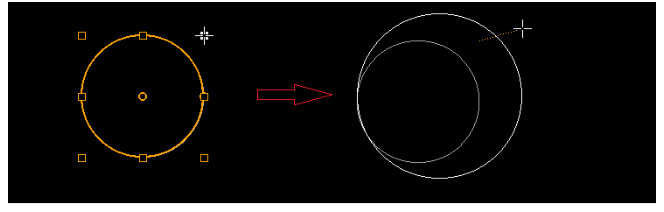
\includegraphics[width=0.92\textwidth]{gui-fig-191.png}
\caption{调整圆形尺寸：拖拽热点（hotspot）以改变尺寸}
\label{fig:gui-191}
\end{figure}

\begin{figure}[htbp]
\centering
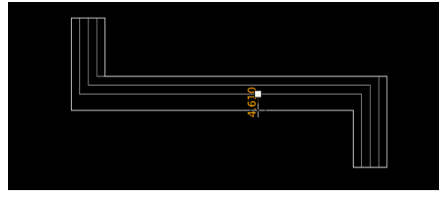
\includegraphics[width=0.92\textwidth]{gui-fig-192.png}
\caption{调整直线：单击并拖拽直线边界以调整线宽}
\label{fig:gui-192}
\end{figure}

\section{删除持久标注}
\subsection*{Removing Persistent Annotations}

要删除某个特定的标注形状：
\begin{enumerate}
  \item 选中该标注形状。
  \item 单击 Delete 工具按钮。
\end{enumerate}

也可以使用 \cmd{remove\_annotation\_shapes [get\_selection]} 命令。

\begin{lstlisting}
icc2_shell> remove_annotation_shapes [get_selection]
\end{lstlisting}

% 第 18 章 Working With Manufacturing Objects
\bichapter{处理制造对象}{Working With Manufacturing Objects}
\label{chap:gui-mfg}

IC Compiler II GUI 可以查看、选择和编辑设计中的下列制造对象。它们参与半导体芯片的制造，因此称为制造对象。
\begin{itemize}
  \item Assembly die：从晶圆上切下之后的物理裸片。
  \item Sealring：比芯片边界更大的矩形晶圆区域，用于保护裸片免受机械损伤。
  \item Stitching zone（Kerf）：把晶圆切开形成裸片时被去除的材料宽度。
\end{itemize}

相关主题：
\begin{itemize}
  \item 选择制造对象
  \item 查询制造对象
  \item 查看制造对象的属性
  \item 编辑制造对象
\end{itemize}

\section{选择制造对象}
\subsection*{Selecting a Manufacturing Object}

可以用下列方式选择制造对象：
\begin{itemize}
  \item 在布局视图中单击该对象；
  \item 在上下文菜单中选择 Related Manufacturing Shapes；
  \item 使用 Select by Name 工具栏。
\end{itemize}

指针停在制造对象上时，工具提示会显示该对象的信息。在布局视图中，用 View Settings 面板控制制造对象的可见性与可选性。

\section{查询制造对象}
\subsection*{Querying Manufacturing Objects}

用 Query 面板搜索制造对象。

\section{查看制造对象的属性}
\subsection*{Viewing the Properties of a Manufacturing Object}

用 Properties 面板查看制造对象的属性。

\section{编辑制造对象}
\subsection*{Editing a Manufacturing Object}

可以在 GUI 中拉伸、添加或切割制造对象。
\begin{enumerate}
  \item 在布局视图中选中对象。
  \item 使用 Edit 菜单中的编辑工具。
\end{enumerate}

在布局视图中编辑对象的方法，见第~\ref{chap:gui-start}~章「编辑物理版图」。

% 第 19 章 Extending the Graphical User Interface
\bichapter{扩展图形用户界面}{Extending the Graphical User Interface}
\label{chap:gui-ext}

IC Compiler II 图形用户界面（GUI）提供一套丰富的应用程序编程接口（application programming interface，API），用于定制菜单、按钮以及 GUI 的其他元素。可用该 API 创建自定义按钮、菜单项（menu item）和地图模式（map mode），并把它们关联到工具中的自定义函数或内建函数。定制可以在工具启动时自动加载，也可以稍后通过 source 脚本文件中的命令来添加。

此外，工具支持标注（annotation）。可用标注在版图视图（layout view）上绘制直线、矩形、多边形、符号和文字。

下列主题说明不同类型的 GUI 定制：
\begin{itemize}
  \item 创建菜单项
  \item 向 Favorites 调色板添加按钮
  \item 用 Tcl 命令高亮对象
  \item 创建标注
  \item 保存标注
  \item 创建新的视觉模式
\end{itemize}

% ============================================================
\section{创建菜单项}
\subsection*{Creating Menu Items}

IC Compiler II 工具通过 \cmd{gui\_create\_menu} 及其他命令支持菜单定制。使用 \cmd{gui\_create\_menu} 命令修改菜单栏（menu bar）并添加新命令；使用 \cmd{gui\_set\_hotkey} 命令定义或重新定义热键（hotkey）。

下列彼此独立的示例逐步增加菜单定制的复杂度，用于建立名为 \textbf{Nudge Left} 与 \textbf{Nudge Right} 的新菜单项。这两项分别把视图略微向左、向右平移（pan）。

\begin{itemize}
  \item 定义两个基本菜单项，见图~\ref{fig:gui-193}。
\end{itemize}

\begin{figure}[htbp]
\centering
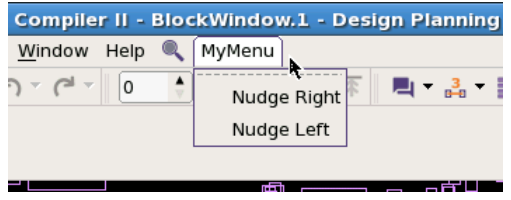
\includegraphics[width=0.92\textwidth]{gui-fig-193.png}
\caption{简单菜单项}
\label{fig:gui-193}
\end{figure}

\begin{lstlisting}
gui_create_menu -menu "MyMenu->Nudge Right" \
   -tcl_cmd {gui_scroll \
   -window [gui_get_current_window -view] -hrel .05}

gui_create_menu -menu "MyMenu->Nudge Left" \
   -tcl_cmd {gui_scroll \
   -window [gui_get_current_window -view] -hrel -.05}
\end{lstlisting}

\begin{itemize}
  \item 在上一例的基础上，为这些菜单项创建标题（heading），并插入一条分隔线（separator），见图~\ref{fig:gui-194}。
\end{itemize}

\begin{figure}[htbp]
\centering
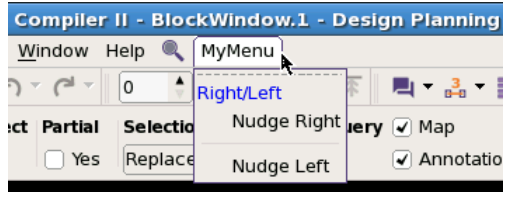
\includegraphics[width=0.92\textwidth]{gui-fig-194.png}
\caption{带标题与分隔线的菜单}
\label{fig:gui-194}
\end{figure}

\begin{lstlisting}
gui_create_menu -menu "MyMenu->Right/Left" -heading "Right/Left"
gui_create_menu -menu "MyMenu->Nudge Right" \
   -tcl_cmd {gui_scroll \
      -window [gui_get_current_window -view] -hrel .05}

gui_create_menu -menu "MyMenu->___" -separator
gui_create_menu -menu "MyMenu->Nudge Left" \
   -tcl_cmd {gui_scroll \
      -window [gui_get_current_window -view] -hrel -.05}
\end{lstlisting}

\begin{itemize}
  \item 在上一例的基础上，把新菜单项放在 \textbf{Help} 菜单左侧一个位置，并为每个菜单项定义自定义图标，见图~\ref{fig:gui-195}。
\end{itemize}

\begin{figure}[htbp]
\centering
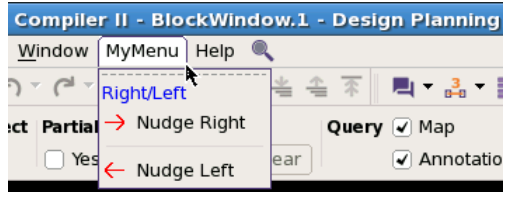
\includegraphics[width=0.92\textwidth]{gui-fig-195.png}
\caption{指定位置的菜单}
\label{fig:gui-195}
\end{figure}

\begin{lstlisting}
gui_create_menu -menu "MyMenu->Right/Left" \
   -heading "Right/Left" \
   -anchor_item Help \
   -anchor_offset -1
gui_create_menu -menu "MyMenu->Nudge Right" \
   -tcl_cmd {gui_scroll \
   -window [gui_get_current_window -view] -hrel .05} \
   -icon_file /u/user/icons/right_16_xpm.xpm
gui_create_menu -menu "MyMenu->___" -separator
gui_create_menu -menu "MyMenu->Nudge Left" \
   -tcl_cmd {gui_scroll \
   -window [gui_get_current_window -view] -hrel -.05} \
   -icon_file /u/user/icons/left_16_xpm.xpm
\end{lstlisting}

\begin{itemize}
  \item 在上一例的基础上，先用 \cmd{gui\_create\_menu} 命令定义菜单项，再用 \cmd{gui\_set\_hotkey} 命令重新定义热键。热键定义会显示在菜单中，见图~\ref{fig:gui-196}。
\end{itemize}

\begin{figure}[htbp]
\centering
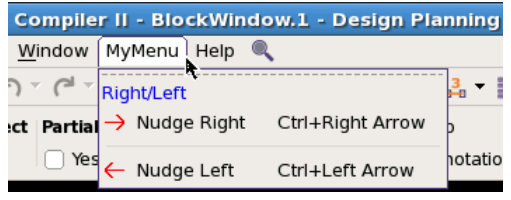
\includegraphics[width=0.92\textwidth]{gui-fig-196.png}
\caption{带热键定义的菜单}
\label{fig:gui-196}
\end{figure}

\begin{lstlisting}
gui_set_hotkey -replace -hot_key Ctrl+Right \
   -menu "MyMenu->Nudge Right"
gui_set_hotkey -replace -hot_key Ctrl+Left \
   -menu "MyMenu->Nudge Left"
\end{lstlisting}

如果热键此前尚未分配，可以用 \cmd{gui\_create\_menu} 命令的 \opt{-hot\_key} 选项来分配。本例使用 \cmd{gui\_set\_hotkey} \opt{-replace} 覆盖已有的热键设置。

% ============================================================
\section{向 Favorites 调色板添加按钮}
\subsection*{Adding Buttons to the Favorites Palette}

可以把按钮添加到收藏夹调色板（Favorites palette）。这是新建工具栏（toolbar）之外的另一种做法。要把一个按钮项加到 Favorites 调色板：
\begin{enumerate}
  \item 按 F10 打开 Favorites 调色板。
  \item 单击某个按钮，并将其拖到 Favorites 调色板上。
\end{enumerate}

要用命令搜索（command search）找到按钮项并加到 Favorites 调色板：
\begin{enumerate}
  \item 按 F10 打开 Favorites 调色板。
  \item 单击放大镜，打开命令搜索。
  \item 输入命令或任务名称。
  \item 在结果列表中单击该项，并将其拖到 Favorites 调色板上。
\end{enumerate}

见图~\ref{fig:gui-197}。

\begin{figure}[htbp]
\centering
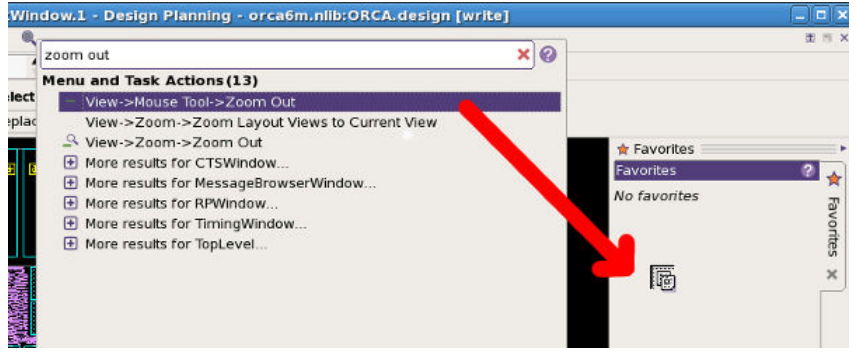
\includegraphics[width=0.92\textwidth]{gui-fig-197.png}
\caption{把按钮拖到 Favorites 调色板}
\label{fig:gui-197}
\end{figure}

% ============================================================
\section{用 Tcl 命令高亮对象}
\subsection*{Highlighting Objects With Tcl Commands}

用 Tcl 命令可以在 GUI 中高亮（highlight）对象，以不同颜色显示，便于识别。也可以定义要着色的对象集合（collection）。

\begin{itemize}
  \item 用三种不同颜色高亮 \cmd{NAND2*}、\cmd{NAND3*} 与 \cmd{NAND4*} 单元，见图~\ref{fig:gui-198}。
\end{itemize}

\begin{lstlisting}
gui_change_highlight -color yellow
   -collection [get_cells -hier -filter "ref_name=~NAND2*"]
gui_change_highlight -color red
   -collection [get_cells -hier -filter "ref_name=~NAND3*"]
gui_change_highlight -color light_blue
   -collection [get_cells -hier -filter "ref_name=~NAND4*"]
\end{lstlisting}

\begin{figure}[htbp]
\centering
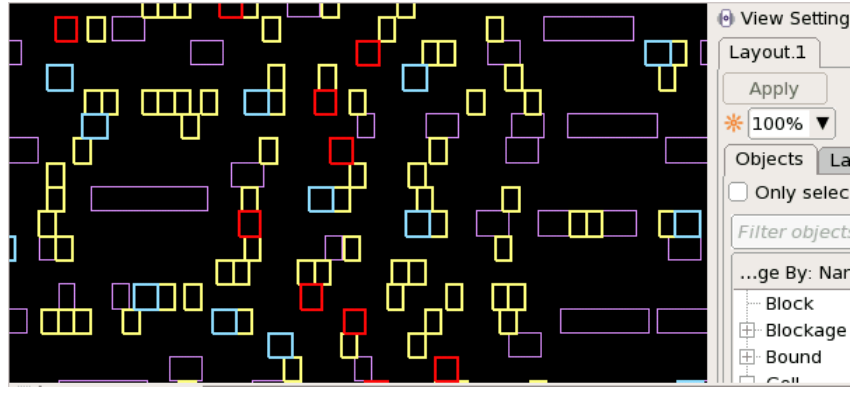
\includegraphics[width=0.92\textwidth]{gui-fig-198.png}
\caption{高亮的单元}
\label{fig:gui-198}
\end{figure}

\begin{itemize}
  \item 删除红色高亮。
\end{itemize}

\begin{lstlisting}
gui_change_highlight -color red -remove
\end{lstlisting}

\begin{itemize}
  \item 删除全部高亮。
\end{itemize}

\begin{lstlisting}
gui_change_highlight -all_colors -remove
\end{lstlisting}

% ============================================================
\section{创建标注}
\subsection*{Creating Annotations}

要向版图视图添加信息，可用标注创建直线、矩形、多边形和文字。标注不会保存到设计数据库，因此不具有持久性。用 \cmd{gui\_add\_annotation} 命令添加标注；用 \cmd{gui\_remove\_annotations} 命令删除标注。要创建持久标注，请使用 \cmd{create\_annotation\_shape} 命令。

\begin{seeAlsoBox}
详见第~\ref{chap:gui-anno}~章「创建持久标注」。
\end{seeAlsoBox}

下列示例创建不同类型的标注。最后一个示例删除全部标注。

\begin{itemize}
  \item 添加一条直线标注，见图~\ref{fig:gui-199}。
\end{itemize}

\begin{lstlisting}
gui_add_annotation -window Layout.1 -type line -color yellow \
   -width 4 {{67 2748} {636 2748}}
\end{lstlisting}

\begin{figure}[htbp]
\centering
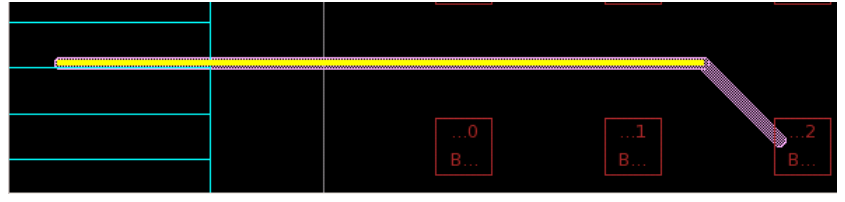
\includegraphics[width=0.92\textwidth]{gui-fig-199.png}
\caption{直线标注}
\label{fig:gui-199}
\end{figure}

\begin{itemize}
  \item 添加一条灰色直线，从单元 \cmd{pad\_iopad\_40} 的中心连到单元 \cmd{left\_15\_2} 的中心，并用十六进制值指定颜色，见图~\ref{fig:gui-200}。
\end{itemize}

\begin{lstlisting}
set cell1 [get_cells pad_iopad_40]
set cell2 [get_cells left_15_2]
gui_add_annotation -window Layout.1 -width 5 -color #999999 \
   -type line [list [list $cell1 center] [list $cell2 center]]
\end{lstlisting}

\begin{figure}[htbp]
\centering
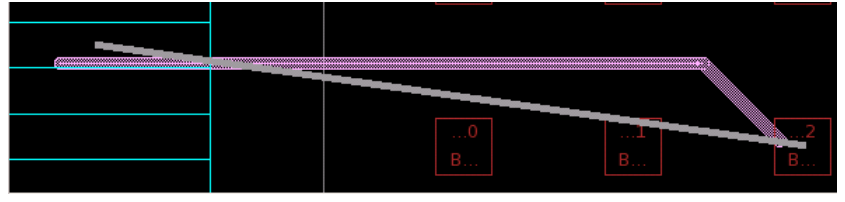
\includegraphics[width=0.92\textwidth]{gui-fig-200.png}
\caption{单元之间的直线标注}
\label{fig:gui-200}
\end{figure}

\begin{itemize}
  \item 添加一条矩形标注，见图~\ref{fig:gui-201}。
\end{itemize}

\begin{lstlisting}
gui_add_annotation -window Layout.1 -type rect -color red \
   -width 4 {{65 2700} {640 2800}}
\end{lstlisting}

\begin{figure}[htbp]
\centering
\includegraphics[width=0.92\textwidth]{gui-fig-201.png}
\caption{矩形标注}
\label{fig:gui-201}
\end{figure}

\begin{itemize}
  \item 添加一条文字标注。必须确保包围盒（bounding box）足够大，能够容纳文字。见图~\ref{fig:gui-202}。
\end{itemize}

\begin{lstlisting}
gui_add_annotation -window Layout.1 -type text -color white \
   -text "RDL Route" {{65 2715} {640 2815}}
\end{lstlisting}

\begin{figure}[htbp]
\centering
\includegraphics[width=0.92\textwidth]{gui-fig-202.png}
\caption{文字标注}
\label{fig:gui-202}
\end{figure}

\begin{itemize}
  \item 添加多条标注，并为每条标注附上信息提示（infotip），见图~\ref{fig:gui-203}。
\end{itemize}

\begin{lstlisting}
set net pad[40]
set shapes [get_shapes -q -of_objects $net]
foreach_in_collection shape $shapes {
  set len [get_attribute $shape length]
  gui_add_annotation -window Layout.1 -type line \
     -color yellow -width 4 \
     -info_tip "RDL Route $net\nLength = $len" \
     [get_attribute $shape points]
}
\end{lstlisting}

\begin{figure}[htbp]
\centering
\includegraphics[width=0.92\textwidth]{gui-fig-203.png}
\caption{带信息提示的标注}
\label{fig:gui-203}
\end{figure}

\begin{itemize}
  \item 添加两个圆形标注，半径均为 100，见图~\ref{fig:gui-204}。
\end{itemize}

\begin{lstlisting}
gui_add_annotation -type circle -color yellow -width 2 \
   -radius 100 {{0 0}}
gui_add_annotation -type circle -color red \
   -width 2 {{200 0} {300 0}}
\end{lstlisting}

\begin{figure}[htbp]
\centering
\includegraphics[width=0.92\textwidth]{gui-fig-204.png}
\caption{圆形标注}
\label{fig:gui-204}
\end{figure}

\begin{itemize}
  \item 创建两个圆形标尺（circular ruler），圆心分别为 (0, 0) 与 (400, 0)，见图~\ref{fig:gui-205}。
\end{itemize}

\begin{lstlisting}
gui_add_annotation -type circular_ruler \
   -color light_green {{0 0} {100 0}}
gui_add_annotation -type circular_ruler \
   -color light_purple {{400 0} {500 0} {700 0}}
\end{lstlisting}

可以再指定若干点，从而以同一圆心创建更多圆形标尺。用 \cmd{gui\_add\_annotation} 命令创建圆形标尺时，会忽略 \opt{-text}、\opt{-pattern}、\opt{-width} 和 \opt{-line\_style} 选项。

\begin{figure}[htbp]
\centering
\includegraphics[width=0.92\textwidth]{gui-fig-205.png}
\caption{圆形标尺}
\label{fig:gui-205}
\end{figure}

\begin{itemize}
  \item 创建一条 45 度角的圆形标尺，见图~\ref{fig:gui-206}。
\end{itemize}

\begin{lstlisting}
gui_add_annotation -type circular_ruler -color light_purple \
   {{0 0} {70.171 70.711} {141.421 141.421}}
\end{lstlisting}

\begin{figure}[htbp]
\centering
\includegraphics[width=0.92\textwidth]{gui-fig-206.png}
\caption{45 度圆形标尺}
\label{fig:gui-206}
\end{figure}

\begin{itemize}
  \item 从当前窗口删除全部标注。
\end{itemize}

\begin{lstlisting}
gui_remove_annotations \
   -window [gui_get_current_window -view -mru]
\end{lstlisting}

\begin{itemize}
  \item 从所有窗口删除全部标注。
\end{itemize}

\begin{lstlisting}
gui_remove_annotations [gui_get_annotations]
\end{lstlisting}

% ============================================================
\section{保存标注}
\subsection*{Saving Annotations}

要把 \cmd{gui\_add\_annotation} 命令创建的标注写到文件，使用 \cmd{gui\_write\_annotations} 命令。默认情况下，\cmd{gui\_write\_annotations} 写出全局标注（global annotation）。要写出当前全部版图标注，请带上参数 \cmd{[gui\_get\_annotations]}。

用下列选项控制 \cmd{gui\_write\_annotations} 命令的输出。
\begin{itemize}
  \item \opt{-file} \cmd{file\_name}：指定输出文件名。
  \item \opt{-append}：把输出追加到指定文件。默认情况下，若用 \opt{-file} 选项指定已存在的文件，命令会发出错误消息。
  \item \opt{-force}：覆盖指定的输出文件。
  \item \opt{-compress} \cmd{gzip}：用 gzip 压缩输出文件。
  \item \cmd{annotations}：指定要写入输出文件的标注。
\end{itemize}

下列示例创建两条标注：从 (0, 0) 到 (200, 200) 的直线标注，以及位于 (0, 0) 的圆形标注。

\begin{noteBox}
第一条标注使用 \opt{-window} 选项指定窗口，第二条标注不带该选项。
\end{noteBox}

\begin{lstlisting}
gui_add_annotation -window Layout.1 -type line -color yellow \
   -width 4 {{0 0} {200 200}}
gui_add_annotation -type circular_ruler \
   -color red {{0 0} {100 0}}
\end{lstlisting}

这些命令在版图中创建下列标注，见图~\ref{fig:gui-207}。

\begin{figure}[htbp]
\centering
\includegraphics[width=0.92\textwidth]{gui-fig-207.png}
\caption{直线与圆形标注}
\label{fig:gui-207}
\end{figure}

\cmd{gui\_write\_annotations} \opt{-file} \cmd{file\_name} \cmd{[gui\_get\_annotations]} 命令写出全部全局标注和特定于窗口的标注。
\begin{lstlisting}
icc2_shell> gui_write_annotations \
   -file all_gui_annotations.tcl [gui_get_annotations]
icc2_shell> sh cat all_gui_annotations.tcl
...
set Layout_1 Layout.1
gui_add_annotation -window $Layout_1 -group global -type polyline \
   -color yellow -pattern NoBrush -line_style SolidLine \
   -width 4 {{0.000 0.000} {200.000 200.000}}
gui_add_annotation -window global -group global \
   -type circular_ruler -color red -pattern NoBrush \
   -line_style SolidLine -width 1 {{0.000 0.000} {100.000 0.000}}
\end{lstlisting}

\cmd{gui\_write\_annotations} \opt{-file} \cmd{file\_name} 命令只写出全局标注（未使用 \opt{-window} 选项指定的标注）。
\begin{lstlisting}
icc2_shell> gui_write_annotations -file global_gui_annotations.tcl
icc2_shell> sh cat global_gui_annotations.tcl
...
gui_add_annotation -window global -group global \
   -type circular_ruler -color red -pattern NoBrush \
   -line_style SolidLine \
   -width 1 {{0.000 0.000} {100.000 0.000}}
\end{lstlisting}

% ============================================================
\section{创建新的视觉模式}
\subsection*{Creating New Visual Modes}

视觉模式（visual mode）以彩色叠层（overlay）高亮设计信息。可用视觉模式高亮设计中的不同元素，并把这些元素组织到各个箱（bin）中。\cmd{gui\_create\_vm} 与 \cmd{gui\_create\_vmbucket} 命令用于定义新的视觉模式、创建单独的箱，并把一个集合关联到每个箱。

下列示例创建一个新的视觉模式，按设计层次（design hierarchy）的不同部分为宏单元（macro）着色。\cmd{gui\_create\_vm} 命令创建名为 \textbf{Macros} 的新视觉模式。启动 \textbf{Macros} 视觉模式后，单击 \textbf{Reload} 按钮时会调用 \cmd{reload\_macros\_vm} 过程（procedure）。\cmd{gui\_create\_vmbucket} 命令把该视觉模式中的各个箱指定到具体集合。\cmd{gui\_show\_map} 命令打开视觉模式调色板（Visual Mode palette），并显示新的 \textbf{Macros} 视觉模式。工具显示出 Visual Mode 调色板后，单击 \textbf{Reload} 按钮即可为宏单元着色。

\begin{seeAlsoBox}
关于 Visual Mode 调色板的更多信息，见第~\ref{chap:gui-map}~章「视觉模式概述」。
\end{seeAlsoBox}

\begin{lstlisting}
gui_create_vm -name Macros -update_cmd reload_macros_vm
proc reload_macros_vm {args} {
  set vm Macros
  gui_remove_vmbucket -vmname $vm -all
  set collection_1 [get_cells -physical_context \
     -filter "is_hard_macro && full_name=~I_CLOCK_GEN/*"]
  set collection_2 [get_cells -physical_context \
     -filter "is_hard_macro && full_name=~I_ORCA_TOP/I_PCI_TOP/*"]
  set collection_3 [get_cells -physical_context \
     -filter "is_hard_macro && full_name=~I_ORCA_TOP/I_CONTEXT_MEM/*"]
  set collection_4 [get_cells -physical_context \
     -filter "is_hard_macro && full_name=~I_ORCA_TOP/I_RISC_CORE/*"]

  gui_create_vmbucket -vmname $vm -name clock_gen \
     -title {clock_gen} -color red -collection $collection_1
  gui_create_vmbucket -vmname $vm -name pci_top \
     -title {pci_top} -color green -collection $collection_2
  gui_create_vmbucket -vmname $vm -name context_mem \
     -title {context_mem} -color blue -collection $collection_3
  gui_create_vmbucket -vmname $vm -name risc_core \
     -title {risc_core} -color yellow -collection $collection_4
}
gui_show_map -map Macros -show true
\end{lstlisting}

见图~\ref{fig:gui-208}。

\begin{figure}[htbp]
\centering
\includegraphics[width=0.92\textwidth]{gui-fig-208.png}
\caption{自定义视觉模式}
\label{fig:gui-208}
\end{figure}


\end{document}
